% Options for packages loaded elsewhere
\PassOptionsToPackage{unicode}{hyperref}
\PassOptionsToPackage{hyphens}{url}
\PassOptionsToPackage{dvipsnames,svgnames,x11names}{xcolor}
%
\documentclass[
  11pt,
  a4paper,
]{book}

\usepackage{amsmath,amssymb}
\usepackage{lmodern}
\usepackage{iftex}
\ifPDFTeX
  \usepackage[T1]{fontenc}
  \usepackage[utf8]{inputenc}
  \usepackage{textcomp} % provide euro and other symbols
\else % if luatex or xetex
  \usepackage{unicode-math}
  \defaultfontfeatures{Scale=MatchLowercase}
  \defaultfontfeatures[\rmfamily]{Ligatures=TeX,Scale=1}
\fi
% Use upquote if available, for straight quotes in verbatim environments
\IfFileExists{upquote.sty}{\usepackage{upquote}}{}
\IfFileExists{microtype.sty}{% use microtype if available
  \usepackage[]{microtype}
  \UseMicrotypeSet[protrusion]{basicmath} % disable protrusion for tt fonts
}{}
\makeatletter
\@ifundefined{KOMAClassName}{% if non-KOMA class
  \IfFileExists{parskip.sty}{%
    \usepackage{parskip}
  }{% else
    \setlength{\parindent}{0pt}
    \setlength{\parskip}{6pt plus 2pt minus 1pt}}
}{% if KOMA class
  \KOMAoptions{parskip=half}}
\makeatother
\usepackage{xcolor}
\setlength{\emergencystretch}{3em} % prevent overfull lines
\setcounter{secnumdepth}{5}
% Make \paragraph and \subparagraph free-standing
\ifx\paragraph\undefined\else
  \let\oldparagraph\paragraph
  \renewcommand{\paragraph}[1]{\oldparagraph{#1}\mbox{}}
\fi
\ifx\subparagraph\undefined\else
  \let\oldsubparagraph\subparagraph
  \renewcommand{\subparagraph}[1]{\oldsubparagraph{#1}\mbox{}}
\fi


\providecommand{\tightlist}{%
  \setlength{\itemsep}{0pt}\setlength{\parskip}{0pt}}\usepackage{longtable,booktabs,array}
\usepackage{calc} % for calculating minipage widths
% Correct order of tables after \paragraph or \subparagraph
\usepackage{etoolbox}
\makeatletter
\patchcmd\longtable{\par}{\if@noskipsec\mbox{}\fi\par}{}{}
\makeatother
% Allow footnotes in longtable head/foot
\IfFileExists{footnotehyper.sty}{\usepackage{footnotehyper}}{\usepackage{footnote}}
\makesavenoteenv{longtable}
\usepackage{graphicx}
\makeatletter
\def\maxwidth{\ifdim\Gin@nat@width>\linewidth\linewidth\else\Gin@nat@width\fi}
\def\maxheight{\ifdim\Gin@nat@height>\textheight\textheight\else\Gin@nat@height\fi}
\makeatother
% Scale images if necessary, so that they will not overflow the page
% margins by default, and it is still possible to overwrite the defaults
% using explicit options in \includegraphics[width, height, ...]{}
\setkeys{Gin}{width=\maxwidth,height=\maxheight,keepaspectratio}
% Set default figure placement to htbp
\makeatletter
\def\fps@figure{htbp}
\makeatother
\newlength{\cslhangindent}
\setlength{\cslhangindent}{1.5em}
\newlength{\csllabelwidth}
\setlength{\csllabelwidth}{3em}
\newlength{\cslentryspacingunit} % times entry-spacing
\setlength{\cslentryspacingunit}{\parskip}
\newenvironment{CSLReferences}[2] % #1 hanging-ident, #2 entry spacing
 {% don't indent paragraphs
  \setlength{\parindent}{0pt}
  % turn on hanging indent if param 1 is 1
  \ifodd #1
  \let\oldpar\par
  \def\par{\hangindent=\cslhangindent\oldpar}
  \fi
  % set entry spacing
  \setlength{\parskip}{#2\cslentryspacingunit}
 }%
 {}
\usepackage{calc}
\newcommand{\CSLBlock}[1]{#1\hfill\break}
\newcommand{\CSLLeftMargin}[1]{\parbox[t]{\csllabelwidth}{#1}}
\newcommand{\CSLRightInline}[1]{\parbox[t]{\linewidth - \csllabelwidth}{#1}\break}
\newcommand{\CSLIndent}[1]{\hspace{\cslhangindent}#1}

\usepackage{amsmath}
\usepackage{booktabs}
\usepackage{caption}
\usepackage{longtable}
\makeatletter
\@ifpackageloaded{tcolorbox}{}{\usepackage[many]{tcolorbox}}
\@ifpackageloaded{fontawesome5}{}{\usepackage{fontawesome5}}
\definecolor{quarto-callout-color}{HTML}{909090}
\definecolor{quarto-callout-note-color}{HTML}{0758E5}
\definecolor{quarto-callout-important-color}{HTML}{CC1914}
\definecolor{quarto-callout-warning-color}{HTML}{EB9113}
\definecolor{quarto-callout-tip-color}{HTML}{00A047}
\definecolor{quarto-callout-caution-color}{HTML}{FC5300}
\definecolor{quarto-callout-color-frame}{HTML}{acacac}
\definecolor{quarto-callout-note-color-frame}{HTML}{4582ec}
\definecolor{quarto-callout-important-color-frame}{HTML}{d9534f}
\definecolor{quarto-callout-warning-color-frame}{HTML}{f0ad4e}
\definecolor{quarto-callout-tip-color-frame}{HTML}{02b875}
\definecolor{quarto-callout-caution-color-frame}{HTML}{fd7e14}
\makeatother
\makeatletter
\makeatother
\makeatletter
\@ifpackageloaded{bookmark}{}{\usepackage{bookmark}}
\makeatother
\makeatletter
\@ifpackageloaded{caption}{}{\usepackage{caption}}
\AtBeginDocument{%
\ifdefined\contentsname
  \renewcommand*\contentsname{Table of contents}
\else
  \newcommand\contentsname{Table of contents}
\fi
\ifdefined\listfigurename
  \renewcommand*\listfigurename{List of Figures}
\else
  \newcommand\listfigurename{List of Figures}
\fi
\ifdefined\listtablename
  \renewcommand*\listtablename{List of Tables}
\else
  \newcommand\listtablename{List of Tables}
\fi
\ifdefined\figurename
  \renewcommand*\figurename{Figure}
\else
  \newcommand\figurename{Figure}
\fi
\ifdefined\tablename
  \renewcommand*\tablename{Table}
\else
  \newcommand\tablename{Table}
\fi
}
\@ifpackageloaded{float}{}{\usepackage{float}}
\floatstyle{ruled}
\@ifundefined{c@chapter}{\newfloat{codelisting}{h}{lop}}{\newfloat{codelisting}{h}{lop}[chapter]}
\floatname{codelisting}{Listing}
\newcommand*\listoflistings{\listof{codelisting}{List of Listings}}
\makeatother
\makeatletter
\@ifpackageloaded{caption}{}{\usepackage{caption}}
\@ifpackageloaded{subcaption}{}{\usepackage{subcaption}}
\makeatother
\makeatletter
\@ifpackageloaded{tcolorbox}{}{\usepackage[many]{tcolorbox}}
\makeatother
\makeatletter
\@ifundefined{shadecolor}{\definecolor{shadecolor}{rgb}{.97, .97, .97}}
\makeatother
\makeatletter
\makeatother
\ifLuaTeX
  \usepackage{selnolig}  % disable illegal ligatures
\fi
\IfFileExists{bookmark.sty}{\usepackage{bookmark}}{\usepackage{hyperref}}
\IfFileExists{xurl.sty}{\usepackage{xurl}}{} % add URL line breaks if available
\urlstyle{same} % disable monospaced font for URLs
% Make links footnotes instead of hotlinks:
\DeclareRobustCommand{\href}[2]{#2\footnote{\url{#1}}}
\hypersetup{
  pdftitle={EUROCONTROL Standard Inputs for Economic Analyses},
  pdfauthor={EUROCONTROL Business Cases team},
  colorlinks=true,
  linkcolor={Maroon},
  filecolor={Maroon},
  citecolor={Blue},
  urlcolor={Blue},
  pdfcreator={LaTeX via pandoc}}

\title{EUROCONTROL Standard Inputs for Economic Analyses}
\author{EUROCONTROL Business Cases team}
\date{4/18/23}

\begin{document}
\frontmatter
\maketitle
\ifdefined\Shaded\renewenvironment{Shaded}{\begin{tcolorbox}[breakable, frame hidden, sharp corners, enhanced, borderline west={3pt}{0pt}{shadecolor}, boxrule=0pt, interior hidden]}{\end{tcolorbox}}\fi

\renewcommand*\contentsname{Table of contents}
{
\hypersetup{linkcolor=}
\setcounter{tocdepth}{2}
\tableofcontents
}
\mainmatter
\bookmarksetup{startatroot}

\hypertarget{about-us}{%
\chapter*{About us}\label{about-us}}
\addcontentsline{toc}{chapter}{About us}

\markboth{About us}{About us}

The EUROCONTROL Business Cases team is a dedicated team of experts that
support stakeholders who need to choose between different solutions and
alternatives, using the best available data. For 20 years, EUROCONTROL
has been providing ATM decision makers with a wide range of regularly
updated Standard Inputs to help them to take rational long-term
investment decision.

\bookmarksetup{startatroot}

\hypertarget{notice-and-disclaimer}{%
\chapter*{Notice and Disclaimer}\label{notice-and-disclaimer}}
\addcontentsline{toc}{chapter}{Notice and Disclaimer}

\markboth{Notice and Disclaimer}{Notice and Disclaimer}

The EUROCONTROL Business Cases team has made every effort to ensure that
the information and analysis contained in this document are as accurate
as possible. Only information from quoted sources has been used and
information relating to named parties has been checked with the parties
concerned. Despite these precautions, should you find any errors or
inconsistencies we would be grateful if you could please bring them to
our attention. Our email address is
\href{mailto:aviation.intelligence@eurocontrol.int}{aviation.intelligence@eurocontrol.int}

This document is published by the EUROCONTROL Business Cases team in the
interest of the exchange of information.

Information contained in this document may not be modified without prior
written permission from the EUROCONTROL Business Cases team.

The views expressed herein do not necessarily respect the official views
or policy of EUROCONTROL, which makes no warranty, either implied or
express, for the information contained in this document, neither does it
assume any legal liability or responsibility for the accuracy,
completeness or usefulness of this information.

\hypertarget{publications}{%
\section*{Publications}\label{publications}}
\addcontentsline{toc}{section}{Publications}

\markright{Publications}

EUROCONTROL Headquarters\\
96 Rue de la Fusée\\
B-1130 BRUSSELS\\
Tel: +32 (0)2 729 1152\\
Fax: +32 (0)2 729 5149\\
E-mail:
\href{mailto:publications@eurocontrol.int}{publications@eurocontrol.int}

\bookmarksetup{startatroot}

\hypertarget{foreword}{%
\chapter*{Foreword}\label{foreword}}
\addcontentsline{toc}{chapter}{Foreword}

\markboth{Foreword}{Foreword}

The first version of the Standard Inputs for EUROCONTROL Economic
Analyses series was launched in 2002 and has been kept alive for 20
years now, with the dedication of several colleagues, in particular
Paula and Desirée who put a lot of effort to this document. Now we took
a new step and launched the latest edition on an online platform to
allow for timely and continuous updates of the values, following the
pace of change in the aviation world.

We would like to show our gratitude to the many different colleagues
that have contributed to this endeavor by helping us develop the values
and bring them online. Trying to name them would be impossible.

We have received valuable remarks and suggestions from all stakeholders
in the aviation value chain. In particular we have benefited from
stakeholders involved in the entire development life cycle, from ideas
to a working system. We strongly believe that this collaboration makes
the EUROCONTROL Standard Inputs for Economic Analyses a robust and
authoritative product.

\bookmarksetup{startatroot}

\hypertarget{introduction}{%
\chapter*{Introduction}\label{introduction}}
\addcontentsline{toc}{chapter}{Introduction}

\markboth{Introduction}{Introduction}

This document provides a set of data commonly used in economic and
financial analyses and appraisals, particulary in the field of ATM.

The aim of this document is to standardise the data used in the
different ATM-related assessments, facilitate the data access for the
different stakeholders involved and contribute to the comparability of
different analyses through relying on the same data.

In this edition (10.1.0) the values have been updated according to the
latest available information, either by adding new data or by adjusting
existing data to inflation, where relevant.

Please note that the standard inputs have been compiled from EUROCONTROL
data and intelligence, from values provided by airspace users, ANSPs,
airports, IATA, EASA and other organisations, and from other relevant
documents which are publicly available.

They are average values and may not be appropriate in all circumstances.
The document also gives details of the sources of information, and
discusses the applicability and use of the values.

This document will remain a living document, and so comments and
suggestions are welcome. Readers are invited to send these to
\href{mailto:aviation.intelligence@eurocontrol.int}{aviation.intelligence@eurocontrol.int}.

\hypertarget{details-per-data-item}{%
\section*{Details per data item}\label{details-per-data-item}}

\markright{Details per data item}

For each standard input, the following information is provided, where
relevant.

\begin{longtable}[]{@{}
  >{\raggedright\arraybackslash}p{(\columnwidth - 2\tabcolsep) * \real{0.3333}}
  >{\raggedright\arraybackslash}p{(\columnwidth - 2\tabcolsep) * \real{0.6667}}@{}}
\toprule()
\begin{minipage}[b]{\linewidth}\raggedright
Section
\end{minipage} & \begin{minipage}[b]{\linewidth}\raggedright
Description
\end{minipage} \\
\midrule()
\endhead
EUROCONTROL recommended values & One or a set of recommended values put
forward by EUROCONTROL for the specific indicator. \\
Description & Any relevant information or details regarding the
recommended value (e.g.~information on how the value was computed, the
limitations on using the value, or other remarks). \\
When to use the input? & A recommendation on when and where the specific
input can be beneficial is provided here. \\
Comments & Any questions or further comments regarding the source or
derivation of the value, for example the degree of confidence in the
values and sources cited. \\
Related inputs & A link to other related standard inputs included in the
document. \\
References & A list of sources used for the specific input. \\
\bottomrule()
\end{longtable}

\bookmarksetup{startatroot}

\hypertarget{sec-conversions}{%
\chapter*{General parameters}\label{sec-conversions}}
\addcontentsline{toc}{chapter}{General parameters}

\markboth{General parameters}{General parameters}

Below are presented some key values used in the Standard Inputs and that
can serve as a reference for other uses.

\hypertarget{inflation}{%
\section*{Inflation}\label{inflation}}
\addcontentsline{toc}{section}{Inflation}

\markright{Inflation}

The inflation levels have been calculated based on the Harmonised Index
of Consumer Prices (HICP)
\protect\hyperlink{ref-eurostat:HICP}{{[}1{]}}, as the yearly difference
in the HICP. The HICP data was extracted from
\href{http://ec.europa.eu/eurostat}{Eurostat} HICP - annual data
(average index and rate of change) database (prc\_hicp\_aind).The annual
change in the index is shown in Table~\ref{tbl-inflation-table}.

\hypertarget{tbl-inflation-table}{}
\begin{longtable}{ccc}
\caption{\label{tbl-inflation-table}Annual average inflation values }\tabularnewline

\toprule
Year & Index & Rate of change \\ 
\midrule
2022 & $118.80$ & $9.19\%$ \\ 
2021 & $108.80$ & $2.84\%$ \\ 
2020 & $105.80$ & $0.36\%$ \\ 
2019 & $105.42$ & $1.47\%$ \\ 
2018 & $103.89$ & $1.89\%$ \\ 
2017 & $101.96$ & $1.71\%$ \\ 
2016 & $100.25$ & $0.25\%$ \\ 
2015 & $100.00$ & $0.10\%$ \\ 
2014 & $99.90$ & $0.55\%$ \\ 
2013 & $99.35$ & $1.50\%$ \\ 
2012 & $97.88$ & $2.64\%$ \\ 
2011 & $95.36$ & $3.10\%$ \\ 
2010 & $92.49$ & $2.09\%$ \\ 
2009 & $90.60$ & $0.98\%$ \\ 
2008 & $89.72$ & $3.54\%$ \\ 
2007 & $86.65$ & $2.34\%$ \\ 
2006 & $84.67$ & $2.20\%$ \\ 
2005 & $82.85$ & $2.17\%$ \\ 
2004 & $81.09$ & $2.01\%$ \\ 
2003 & $79.49$ & $1.96\%$ \\ 
2002 & $77.96$ & $2.08\%$ \\ 
2001 & $76.37$ & $2.19\%$ \\ 
2000 & $74.73$ & $1.90\%$ \\ 
\bottomrule
\end{longtable}

\hypertarget{exchange-rates}{%
\section*{Exchange Rate Conversion}\label{exchange-rates}}
\addcontentsline{toc}{section}{Exchange Rate Conversion}

\markright{Exchange Rate Conversion}

The currency exchange rates provided in
Table~\ref{tbl-eurostat-exchange-rates} are based on the European
Central Bank (ECB) rates that are published daily
\protect\hyperlink{ref-ECB:exchange_rates}{{[}2{]}}. The rates shown in
Table~\ref{tbl-eurostat-exchange-rates} correspond to the average rate
for the year 2021 as published by ECB.

\hypertarget{tbl-eurostat-exchange-rates}{}
\begin{longtable}{lcc}
\caption{\label{tbl-eurostat-exchange-rates}Average euro foreign exchange rate (2021) }\tabularnewline

\toprule
Currency & Currency-€ & €-Currency \\ 
\midrule
USD & 0.89 & 1.12 \\ 
GBP & 1.22 & 0.82 \\ 
\bottomrule
\end{longtable}

\hypertarget{cost-of-fuel}{%
\section*{Cost of fuel}\label{cost-of-fuel}}
\addcontentsline{toc}{section}{Cost of fuel}

\markright{Cost of fuel}

The cost of fuel used in this document is based on the 2021 average jet
fuel price handled by IATA
\protect\hyperlink{ref-iata:JetFuelPrice}{{[}3{]}}, unless otherwise
specified. All conversions are done using the values specified on this
page.

\hypertarget{tbl-cost-of-fuel}{}
\begin{longtable}{lccc}
\caption{\label{tbl-cost-of-fuel}Average jet fuel price }\tabularnewline

\toprule
Currency & Price per barrel & Price per gallon & Price per kg \\ 
\midrule
USD & 141.7 & 3.8 & 1.1 \\ 
EUR & 138.9 & 3.3 & 1.1 \\ 
\bottomrule
\end{longtable}

\hypertarget{conversion-values}{%
\section*{Conversion values}\label{conversion-values}}
\addcontentsline{toc}{section}{Conversion values}

\markright{Conversion values}

\hypertarget{tbl-conversion-values}{}
\begin{longtable}{ll}
\caption{\label{tbl-conversion-values}Units conversion values }\tabularnewline

\toprule
From & To \\ 
\midrule
1 nautical mile (NM) & 1.852 km \\ 
1 kilometre (km) & 0.53996 NM \\ 
1 tonne (metric = 1 000 kg) of jet fuel & 325.33 US gallons \\ 
 & 1 235 litres \\ 
 & 7.8 barrels \\ 
1 barrel (bbl) of jet fuel & 42 US gallons \\ 
 & 158.99 litres \\ 
 & 0.1291 tonne = 129.10 kg \\ 
1 US gallon of jet fuel (US gal) & 3.7854 litres \\ 
 & 3.073 kg \\ 
 & 6.7764 lb \\ 
Density of kerosene & 0.812 kg/litre \\ 
1 litre of fuel (l) & 0.26417 US gallons \\ 
1 kilogramme of fuel (kg) & 2.2046 lb \\ 
1 pound of fuel (lb) & 0.45359 kg \\ 
\bottomrule
\end{longtable}

\hypertarget{references}{%
\section*{References}\label{references}}
\addcontentsline{toc}{section}{References}

\markright{References}

\bookmarksetup{startatroot}

\hypertarget{sec-geographical-areas}{%
\chapter*{Geographical areas}\label{sec-geographical-areas}}
\addcontentsline{toc}{chapter}{Geographical areas}

\markboth{Geographical areas}{Geographical areas}

\hypertarget{member-states-and-geographical-areas-covered}{%
\section*{Member States and geographical areas
covered}\label{member-states-and-geographical-areas-covered}}
\addcontentsline{toc}{section}{Member States and geographical areas
covered}

\markright{Member States and geographical areas covered}

Single European Sky initiative and the European Civil Aviation
Conference (ECAC) are the different scopes that are covered in Standard
Inputs document.

\begin{figure}

{\centering 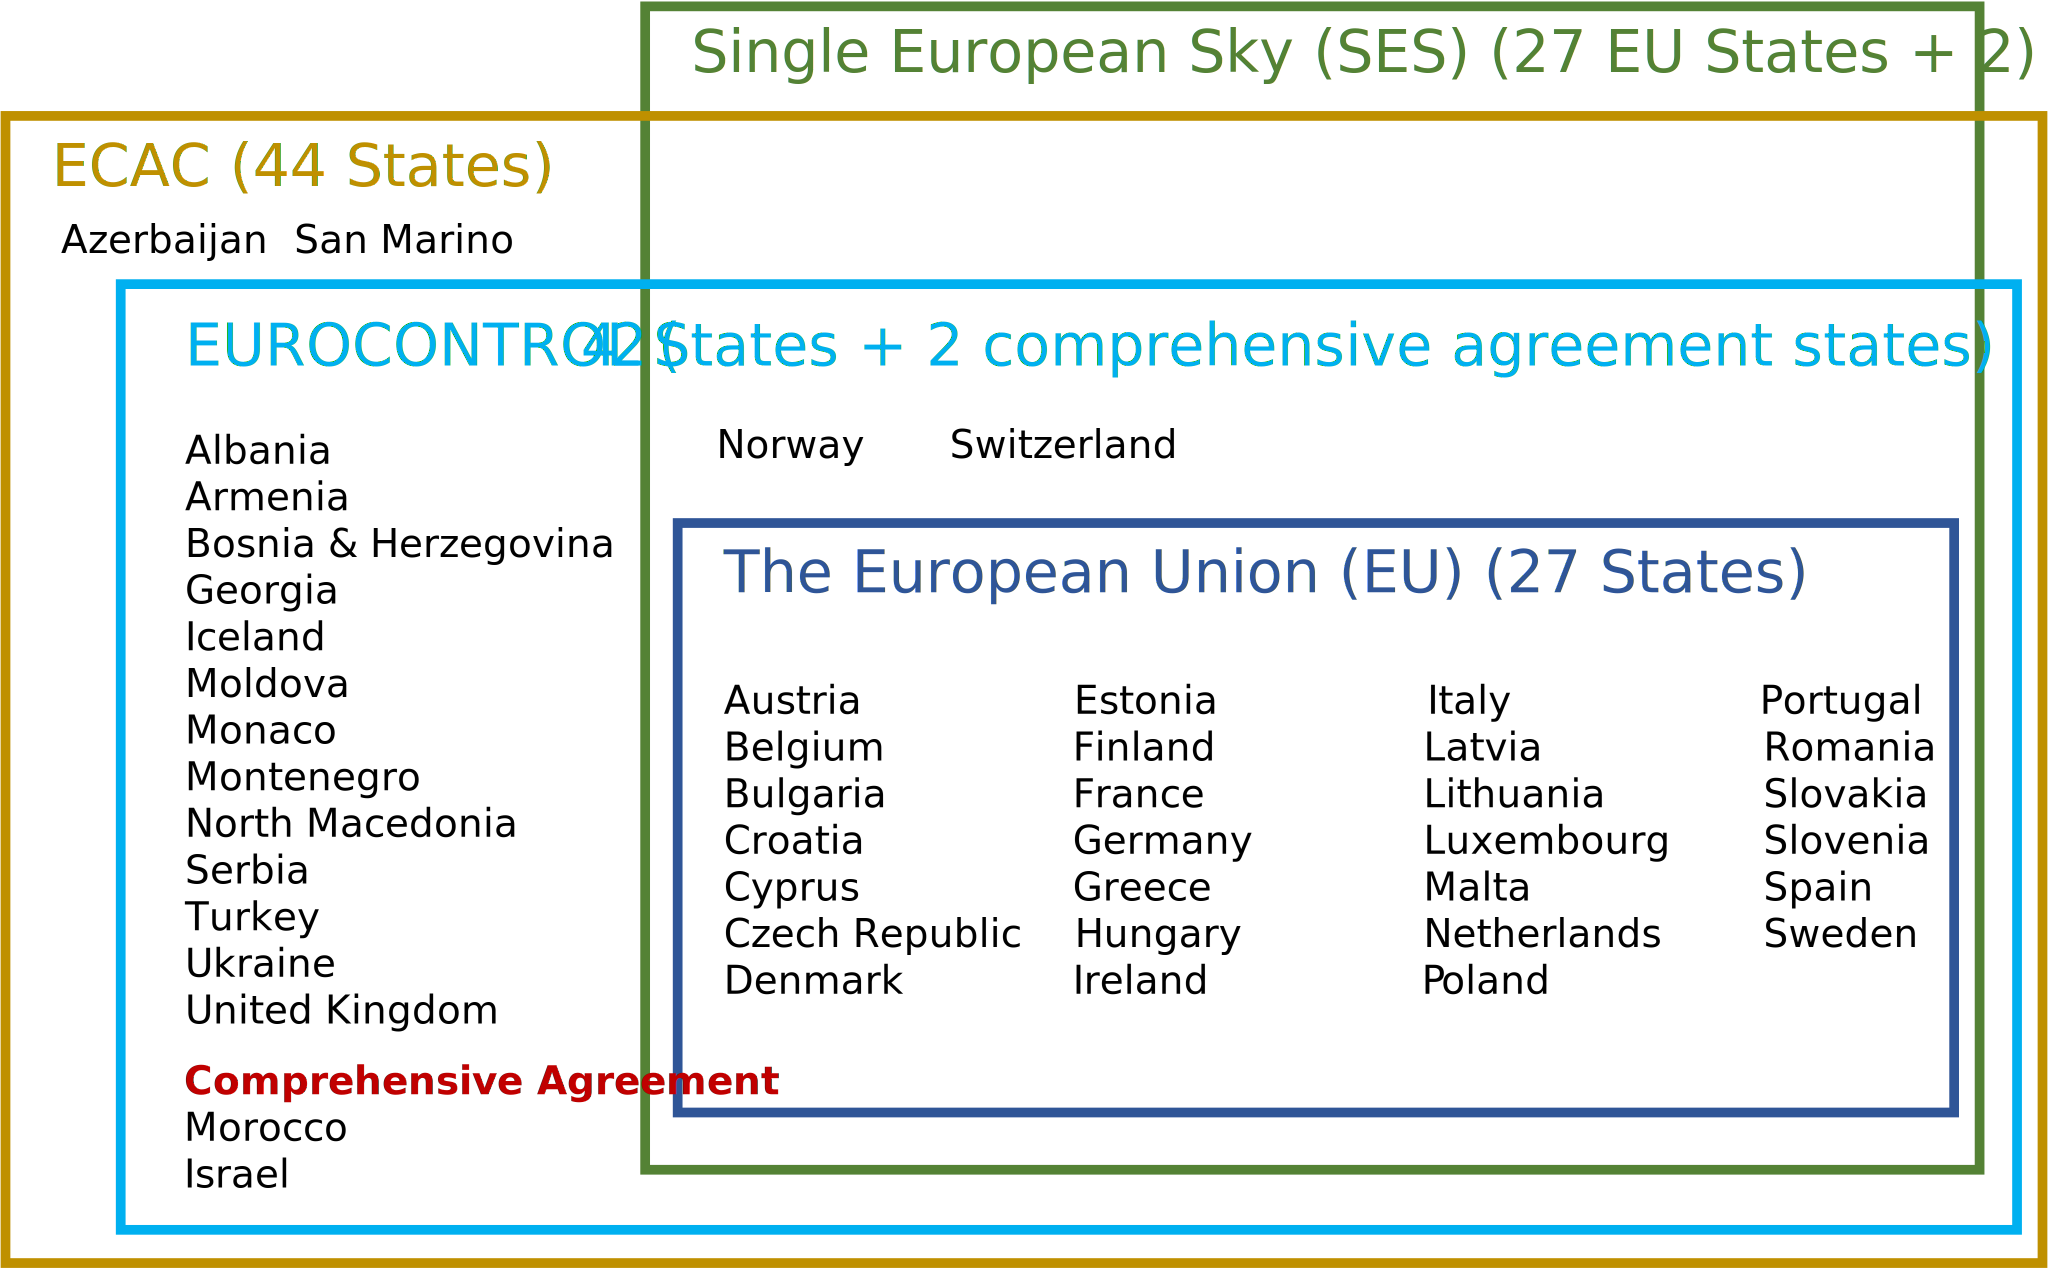
\includegraphics{chapters/../figures/eu_orgs.png}

}

\caption{\label{fig-member-states-set-diagram}State grouping}

\end{figure}

\hypertarget{eurocontrol-member-states}{%
\section*{EUROCONTROL Member States}\label{eurocontrol-member-states}}
\addcontentsline{toc}{section}{EUROCONTROL Member States}

\markright{EUROCONTROL Member States}

\begin{figure}

{\centering \includegraphics{chapters/../figures/eurocontrol_ms.png}

}

\caption{\label{fig-eurocontrol-member-states}EUROCONTROL Member States
(status: November 2020)}

\end{figure}

\hypertarget{airspace-of-the-ecac-member-states}{%
\section*{Airspace of the ECAC Member
States}\label{airspace-of-the-ecac-member-states}}
\addcontentsline{toc}{section}{Airspace of the ECAC Member States}

\markright{Airspace of the ECAC Member States}

ECAC is an intergovernmental organisation that was established by ICAO
and the Council of Europe. ECAC now has 44 Member States, including all
27 EU Member States, 31 of the 32 European Aviation Safety Agency Member
States, and all 41 EUROCONTROL Member States. The figure below is a
graphical representation of the airspace belonging to the ECAC states.

\begin{figure}

{\centering \includegraphics{chapters/../figures/ecac_airspace_fir.png}

}

\caption{\label{fig-ecac-airspace-fir}Airspace controlled by ECAC Member
States}

\end{figure}

\part{Traffic and capacity}

\hypertarget{sec-air-traffic-statistics-and-forecasts}{%
\chapter{Air traffic statistics and
forecasts}\label{sec-air-traffic-statistics-and-forecasts}}

\hypertarget{eurocontrol-recommended-value}{%
\section{EUROCONTROL recommended
value}\label{eurocontrol-recommended-value}}

The Statistics and Forecasts (STATFOR) service produces flights and
service units forecasts of future network traffic with a view to help
planners understand and manage risks, identify bottlenecks and
anticipate the needs of airspace users.

\hypertarget{medium-term-forecasts-7-year-timespan}{%
\subsection{Medium-term forecasts (7-year
timespan)}\label{medium-term-forecasts-7-year-timespan}}

The 7-year forecasts give a comprehensive picture of anticipated air
traffic development in Europe for the next seven years. They combine
flight statistics with economic growth and models of other industry
drivers, including costs, airport capacity, passenger numbers, load
factors and aircraft size. Using high and low growth scenarios, they
present a likely range for growth, to help planners manage risks. They
are published biannually, in spring and autumn, covering flights, en
route and terminal service units.

\begin{figure}

{\centering \includegraphics{chapters/../figures/forecast_2022-2028.png}

}

\caption{\label{fig-forecast-2022-2028-plot}EUROCONTROL 7-year forecast
2022-2028 (October 2022 release)
\protect\hyperlink{ref-statfor:7year_forecast:2022-2028}{{[}4{]}}}

\end{figure}

The above graph shows the traffic forecast taking account of the impact
of the COVID-19 pandemic. In the base scenario, IFR flights are expected
to get back to 2019 levels by 2025.

Traffic statistics and forecasts can be obtained directly from the
STATFOR Interactive Dashboard
(SID)\protect\hyperlink{ref-ectrl:statfor:sid}{{[}5{]}}.

\hypertarget{long-term-forecasts-20-to-30-year-timespan}{%
\subsection{Long-term forecasts (20 to 30-year
timespan)}\label{long-term-forecasts-20-to-30-year-timespan}}

Twenty/thirty-year forecasts: These forecasts look at a range of
distinct possible scenarios for how the air traffic industry might look
in 20-30 years' time. This allows a range of \emph{what if?} questions
to be explored, for factors inside the industry (e.g.~the growth of
small business jets, or of point-to-point traffic) or outside the
industry (e.g.~the price of oil or environmental constraints).
Twenty/thirty-year forecasts are usually published every two to three
years. In April 2022, EUROCONTROL published its first EUROCONTROL
Aviation Outlook (EAO) looking out to 2050, much further than previous
forecasts. This forecast estimates a future number of flights and CO2
emissions per scenario, in line with aviation's objective of achieving
net-zero CO2 emissions by that date.

\begin{figure}

{\centering \includegraphics{chapters/../figures/eao_2050_flights_base_scenario.png}

}

\caption{\label{fig-Forecast-2050-plot}Flight forecast for Europe, with
total growth between 2019 and 2050}

\end{figure}

In the most-likely Base scenario, the forecast is for 16 million flights
in Europe in 2050, 44\% more than in 2019 -- average growth of 1.2\% per
year.

\begin{figure}

{\centering \includegraphics{chapters/../figures/eao_2050_base_scenario.png}

}

\caption{\label{fig-co2-emissions-plot}Estimated CO2 emissions between
2005 and 2050 \protect\hyperlink{ref-aviation:outlook2022}{{[}6{]}}}

\end{figure}

The graph in Figure~\ref{fig-co2-emissions-plot} estimates that by 2050,
CO2 emissions, net of SAF, fleet and operational improvements, are
reduced by about 41\% compared to 2005 in the Base scenario.

\hypertarget{service-units-forecasts}{%
\subsection{Service units forecasts}\label{service-units-forecasts}}

Service Units are billed to airlines for the provision of air-traffic
services. They are of two types:

\begin{itemize}
\item
  En-route service units (TSU) that are taxed for the provision of
  en-route air traffic control and are a function of the weight and the
  distance flown within each state over which the concerned aircraft
  flies.
\item
  Terminal Navigation Service Units (TNSU) are taxed for the provision
  of ground services to the airlines for each departure at a given
  airport. They are a function of the weight of the considered aircraft.
\end{itemize}

EUROCONTROL produces a 7-year forecast of Service Units that builds on
the 7-year IFR movements forecast, to which forecasts of the aircraft
weights and distances are added. This Service Units forecast is provided
as a service to states that are part of the Central Route Charges Office
(CRCO) to help them set-up their en-route units rates, if needed. The
Forecast of Service Units in general serves also as a benchmark for the
European Commission to assess the financial aspects of the performance
plans of the states that are bound by the performance and Charging
Scheme according to EU regulations (EU) N°390/201, N°391/2013.

\begin{figure}

{\centering 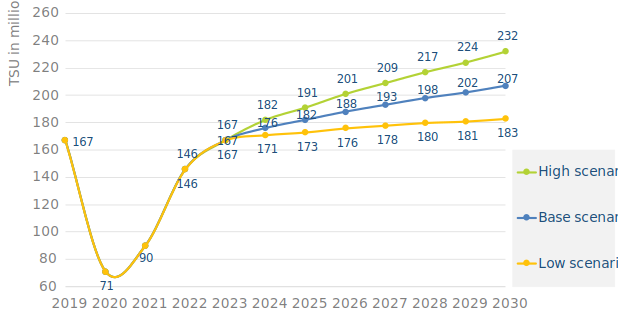
\includegraphics{chapters/../figures/forecast_service_units.png}

}

\caption{\label{fig-forecast-service-units-plot}En-route Service Units
7-year Forecast 2022-2028
\protect\hyperlink{ref-statfor:7year_forecast:2022-2028}{{[}4{]}}}

\end{figure}

The above graph (status: October 2022) shows the en-route service units
forecast taking account of the impact of the COVID-19 pandemic.

\hypertarget{when-to-use-the-inputs}{%
\section{When to use the inputs?}\label{when-to-use-the-inputs}}

The objective of STATFOR is to provide statistics and forecasts on IFR
flight movements and service units in Europe (ECAC) and to monitor and
analyse the evolution of the air transport industry.

\hypertarget{related-inputs}{%
\section{Related inputs}\label{related-inputs}}

Chapter~\ref{sec-medium-term-capacity-planning}
\protect\hyperlink{sec-medium-term-capacity-planning}{Medium-term
capacity planning}

Chapter~\ref{sec-air-traffic-delay}
\protect\hyperlink{sec-air-traffic-delay}{Air traffic delay}

Chapter~\ref{sec-cost-of-delay}
\protect\hyperlink{sec-cost-of-delay}{Cost of delay}

\hypertarget{references-1}{%
\section{References}\label{references-1}}

\hypertarget{sec-medium-term-capacity-planning}{%
\chapter{Medium-term capacity
planning}\label{sec-medium-term-capacity-planning}}

\hypertarget{eurocontrol-recommended-sources}{%
\section{EUROCONTROL recommended
sources}\label{eurocontrol-recommended-sources}}

In this document, capacity planning represents the systematic
determination of resource requirements for the projected output over a
specific period of time. It is a dynamic activity that relies on
constantly changing data on the ATM network use, capacity forecasts,
etc.

Given this, below are presented the sources that are recommended to
consult in order to obtain relevant up to date information on capacity
planning.

\begin{itemize}
\item
  \emph{EUROCONTROL NMD (2022), European Network Operations Plan
  2022-2026} \protect\hyperlink{ref-ectrl:nop:2022}{{[}7{]}} provides a
  short- to medium-term outlook of the expected ATM network operations
  and performance at network and local level.

  It provides a detailed overview of capacity and flight efficiency
  enhancement measures planned at network level and by each Area Control
  Centre (ACC), a description of the airport performance assessment and
  improvement measures planned at airports generating a high level of
  delay, operational actions planned to be taken by the Network Manager
  and other stakeholders that would respond to the performance targets.
  Furthermore, it provides an assessment of the expected impact from
  these measures on the network.
\item
  \emph{EUROCONTROL NMD (2023), European Network Operations Plan (NOP)
  -- Rolling Seasonal Plan}
  \protect\hyperlink{ref-ectrl:nop:rsp}{{[}8{]}}

  The European NOP Rolling Seasonal Plan is updated every Friday,
  focusing on the planning of the next six weeks and on the management
  of the execution and implementation of the 5-years NOP. Its aim is to
  facilitate ANSPs and airports planning to match traffic demand in a
  safe, efficient and coordinated manner by providing them with a
  consolidated European network view of the evolution of air traffic.
  More information about network performance (and access to dashboards
  and the archive) can be found at the
  \href{https://www.eurocontrol.int/network-performance}{Network
  Performance page}.
\item
  \emph{European ATM Master Plan - implementation plan -- level 3}
  \protect\hyperlink{ref-ectrl:mp:ip}{{[}9{]}} and \emph{European ATM
  Master Plan -- implementation report -- level 3}
  \protect\hyperlink{ref-ectrl:mp:ir}{{[}10{]}}

  The \textbf{European ATM Master Plan Level 3 (MPL3) Implementation
  Plan} brings together the framework for the commonly agreed actions
  that ECAC+ Stakeholders should take in the context of the
  implementation of SESAR. These actions are consolidated in
  implementation objectives addressing elements in SESAR which have
  reached the necessary operational and technical maturity and for which
  stakeholders have expressed an interest in their operational
  introduction. They provide all civil and military implementing parties
  (ANSPs, Airport Operators, Airspace Users and Regulators) with a basis
  for short- to medium-term implementation planning. In this respect, it
  addresses:

  \begin{itemize}
  \item
    V3 validated SESAR Solutions
  \item
    CP1 ATM Functionalities (AFs), based on Commission IR (EU) 2021/116
    on Common Project One
  \item
    SESAR Baseline elements, validated or under deployment at the
    beginning of the SESAR Deployment phase
  \item
    SES and ICAO requirements
  \end{itemize}

  Updated yearly, the Plan covers a short to medium-term horizon of
  around 5 years ahead. It is based on the ATM MP L1 and L2, the SESAR
  Deployment Programme (SDP), the Network Strategy Plan (NSP), and the
  SES Interoperability Regulations. In turn, the MPL3 Implementation
  Plan feeds the LSSIP+ monitoring mechanism as well as the reporting
  process through the yearly elaboration of the MPL3 Implementation
  Report. The MPL3 Plan 2022 edition mirrors the content of the SESAR
  Deployment Programme (SDP) for what concerns the IR (EU) 2021/116 on
  the Common Project 1 (CP1). It covers 97 Solutions from SESAR1,
  SESAR2020 W1 and W2 and 97 Implementation Objectives.
\item
  \emph{Local Single Sky ImPlementation (LSSIP) documents}
  \protect\hyperlink{ref-ectrl:lssip}{{[}11{]}}

  The Local Single Sky ImPlementation (LSSIP) documents give a
  comprehensive overview of all ATM information for each of the ECAC
  Member States. They also show the ATM capacity forecasts and planning
  targets from NOP. The documents reflect progress made and detail the
  plans for each State for the next five to seven years. LSSIP
  documents, one for each State, are derived from the European Single
  Sky Implementation (ESSIP) (also known as Master Plan Level 3)
  objectives, and stakeholder lines of action cascade down into the
  States.
\end{itemize}

\hypertarget{related-inputs-1}{%
\section{Related inputs}\label{related-inputs-1}}

Chapter~\ref{sec-air-traffic-statistics-and-forecasts}
\protect\hyperlink{sec-air-traffic-statistics-and-forecasts}{Air traffic
statistics and forecasts}

Chapter~\ref{sec-air-traffic-delay}
\protect\hyperlink{sec-air-traffic-delay}{Air traffic delay}

\hypertarget{references-2}{%
\section{References}\label{references-2}}

\hypertarget{sec-number-of-ifr-flights}{%
\chapter{Number of IFR flights}\label{sec-number-of-ifr-flights}}

\hypertarget{eurocontrol-recommended-values}{%
\section{EUROCONTROL recommended
values}\label{eurocontrol-recommended-values}}

This section presents the evolution of flight movements in Europe (ECAC
area) by flight flow, market segment and aircraft type.

\hypertarget{evolution-of-flights-per-flow-in-2021-compared-to-2019}{%
\subsection{Evolution of flights per flow in 2021 compared to
2019}\label{evolution-of-flights-per-flow-in-2021-compared-to-2019}}

\hypertarget{tbl-ifr-flights-month}{}
\setlength{\LTpost}{0mm}
\begin{longtable}{lrrrrrrc}
\caption{\label{tbl-ifr-flights-month}Evolution of IFR flights in Europe (ECAC) 2019 vs 2021 }\tabularnewline

\toprule
 & \multicolumn{4}{c}{DAIO} & \multicolumn{2}{c}{Total} &  \\ 
\cmidrule(lr){2-5} \cmidrule(lr){6-7}
Month & Departure & Arrival & Internal & Overflight & 2021 & 2019 & 2021 traffic as \% of 2019 \\ 
\midrule
January & $34,972$ & $35,151$ & $206,217$ & $8,984$ & $285,324$ & $787,503$ & $36\%$ \\ 
February & $30,885$ & $30,871$ & $180,689$ & $7,469$ & $249,914$ & $737,763$ & $34\%$ \\ 
March & $37,184$ & $37,174$ & $223,117$ & $9,606$ & $307,081$ & $846,442$ & $36\%$ \\ 
April & $37,685$ & $37,729$ & $241,842$ & $10,136$ & $327,392$ & $906,539$ & $36\%$ \\ 
May & $38,615$ & $38,847$ & $291,508$ & $11,444$ & $380,414$ & $985,862$ & $39\%$ \\ 
June & $45,275$ & $45,437$ & $415,450$ & $12,667$ & $518,829$ & $1,038,128$ & $50\%$ \\ 
July & $62,163$ & $62,118$ & $574,282$ & $13,735$ & $712,298$ & $1,092,562$ & $65\%$ \\ 
August & $64,666$ & $64,778$ & $619,233$ & $14,469$ & $763,146$ & $1,080,554$ & $71\%$ \\ 
September & $61,857$ & $61,777$ & $591,118$ & $13,570$ & $728,322$ & $1,034,322$ & $70\%$ \\ 
October & $64,303$ & $64,142$ & $575,242$ & $15,193$ & $718,880$ & $980,049$ & $73\%$ \\ 
November & $59,573$ & $59,498$ & $483,850$ & $15,986$ & $618,907$ & $801,961$ & $77\%$ \\ 
December & $59,797$ & $59,552$ & $485,033$ & $15,863$ & $620,245$ & $793,617$ & $78\%$ \\ 
Total & $596,975$ & $597,074$ & $4,887,581$ & $149,122$ & $6,230,752$ & $11,085,302$ & $56\%$ \\ 
\bottomrule
\end{longtable}
\begin{minipage}{\linewidth}
\emph{Source: \href{https://www.eurocontrol.int/dashboard/statfor-interactive-dashboard}{STATFOR Interactive Dashboard}}\\
\end{minipage}

Please note that the comparison between 2021 and 2019 in
Table~\ref{tbl-ifr-flights-month} is due to the fact that 2019 is the
last year where the traffic levels were not affected by the COVID-19
pandemic, allowing for a more realistic comparison of the flight
levels.\protect\hyperlink{ref-ectrl:statfor:sid}{{[}5{]}}

\hypertarget{flights-by-market-segment-in-europe-ecac-in-2021-compared-to-2019}{%
\subsection{Flights by market segment in Europe (ECAC) in 2021 compared
to
2019}\label{flights-by-market-segment-in-europe-ecac-in-2021-compared-to-2019}}

\hypertarget{tbl-flights-per-market-segment}{}
\setlength{\LTpost}{0mm}
\begin{longtable}{lrcrcrc}
\caption{\label{tbl-flights-per-market-segment}Flights by market segment in Europe (ECAC) 2019-2021 }\tabularnewline

\toprule
Market segment & 2019 & Share of Total 2019 & 2020 & Share of Total 2020 & 2021 & Share of Total 2021 \\ 
\midrule
Mainline & $3,991,685$ & $36\%$ & $1,479,557$ & $30\%$ & $1,816,909$ & $29\%$ \\ 
Lowcost & $3,493,913$ & $32\%$ & $1,243,422$ & $25\%$ & $1,610,239$ & $26\%$ \\ 
Regional Aircraft & $1,643,854$ & $15\%$ & $746,765$ & $15\%$ & $861,587$ & $14\%$ \\ 
Business Aviation & $683,473$ & $6\%$ & $513,628$ & $10\%$ & $709,398$ & $11\%$ \\ 
All-Cargo & $368,362$ & $3\%$ & $389,914$ & $8\%$ & $419,824$ & $7\%$ \\ 
Other Types & $372,796$ & $3\%$ & $309,283$ & $6\%$ & $363,712$ & $6\%$ \\ 
Charter & $382,218$ & $3\%$ & $162,798$ & $3\%$ & $303,384$ & $5\%$ \\ 
Military & $149,001$ & $1\%$ & $133,711$ & $3\%$ & $145,699$ & $2\%$ \\ 
Total & $11,085,302$ & $100\%$ & $4,979,078$ & $100\%$ & $6,230,752$ & $100\%$ \\ 
\bottomrule
\end{longtable}
\begin{minipage}{\linewidth}
\emph{Source: \href{https://www.eurocontrol.int/dashboard/statfor-interactive-dashboard}{STATFOR Interactive Dashboard}}\\
\end{minipage}

EUROCONTROL market segments were updated in 2022 and saw the
``Traditional Scheduled'' segment split into ``Mainline'' and
``Regional'' according to EUROCONTROL Market Segment Rules
\protect\hyperlink{ref-ectl:market:seg:2022}{{[}12{]}}.

In 2021 the total number of flights went up 25.1\% compared to 2020, but
was at 56.2\% of 2019 flight levels (pre-COVID-19). Compared with 2019,
only two segments increased in 2021 and they were All-Cargo (+13.9\%)
and Business Aviation (+3.8\%). The Mainline (-54.5\%), Low-Cost
(-53.9\%) and Regional (-47.6\%) segments were the most affected, along
with the Charter segment which went down by -20.6\% in 2021 (vs 2019).

\hypertarget{top-20-number-of-flights-by-civil-aviation-aircraft-in-europe-ecac-in-2021}{%
\subsection{Top 20 number of flights by civil aviation aircraft in
Europe (ECAC) in
2021}\label{top-20-number-of-flights-by-civil-aviation-aircraft-in-europe-ecac-in-2021}}

\hypertarget{tbl-flights-per-aircraft-type}{}
\setlength{\LTpost}{0mm}
\begin{longtable}{lrcc}
\caption{\label{tbl-flights-per-aircraft-type}Top 20 flights by aircraft type in Europe (ECAC) in 2021 }\tabularnewline

\toprule
Aircraft Type & Flights & Proportion & Cumulative \\ 
\midrule
B738 & $1,098,879$ & $19\%$ & $19\%$ \\ 
A320 & $760,204$ & $13\%$ & $32\%$ \\ 
A319 & $312,864$ & $5\%$ & $38\%$ \\ 
A20N & $310,527$ & $5\%$ & $43\%$ \\ 
A321 & $193,590$ & $3\%$ & $47\%$ \\ 
A21N & $150,955$ & $3\%$ & $49\%$ \\ 
B77W & $132,040$ & $2\%$ & $51\%$ \\ 
E190 & $131,891$ & $2\%$ & $54\%$ \\ 
AT76 & $109,491$ & $2\%$ & $56\%$ \\ 
B789 & $98,893$ & $2\%$ & $57\%$ \\ 
AT75 & $85,711$ & $1\%$ & $59\%$ \\ 
A333 & $82,982$ & $1\%$ & $60\%$ \\ 
DH8D & $81,496$ & $1\%$ & $62\%$ \\ 
E195 & $76,625$ & $1\%$ & $63\%$ \\ 
B734 & $76,322$ & $1\%$ & $64\%$ \\ 
B77L & $65,577$ & $1\%$ & $66\%$ \\ 
B38M & $63,990$ & $1\%$ & $67\%$ \\ 
CRJ9 & $63,696$ & $1\%$ & $68\%$ \\ 
B737 & $62,673$ & $1\%$ & $69\%$ \\ 
DH8A & $62,082$ & $1\%$ & $70\%$ \\ 
Other types & $1,730,263$ & $30\%$ & $100\%$ \\ 
Total & $5,750,751$ & $100\%$ & NA \\ 
\bottomrule
\end{longtable}
\begin{minipage}{\linewidth}
\emph{Source: \href{https://www.eurocontrol.int/forecasting}{EUROCONTROL STATFOR}}\\
\end{minipage}

In 2021 there were 301 different civil aircraft types operating IFR
flights in Europe. About 70\% of the flights were carried out by the 20
aircraft types listed in Table~\ref{tbl-flights-per-aircraft-type}.
Please note that the values presented in
Table~\ref{tbl-flights-per-aircraft-type} focuses on the civil aviation
flights (i.e.~excluding the military and other categories), resulting in
a difference in the total flights as compared with
Table~\ref{tbl-flights-per-market-segment} and
Table~\ref{tbl-ifr-flights-month}.

\hypertarget{daily-average-of-ifr-flights-2016-to-2021}{%
\subsection{Daily average of IFR flights, 2016 to
2021}\label{daily-average-of-ifr-flights-2016-to-2021}}

Figure~\ref{fig-average-daily-ifr-flights-plot} shows the daily average
number of IFR flights \textbf{EU-wide} between 2016 and 2021.

\begin{figure}

{\centering \includegraphics{chapters/../figures/average_daily_flights.png}

}

\caption{\label{fig-average-daily-ifr-flights-plot}Daily average numbers
of IFR flights \protect\hyperlink{ref-prb:dashboard:2022}{{[}13{]}}}

\end{figure}

\hypertarget{when-to-use-the-input}{%
\section{When to use the input?}\label{when-to-use-the-input}}

This input is recommended to be used in situations where an overview of
the historical evolution in the number of flights is required, namely
grouped according to different criteria.

\hypertarget{related-inputs-2}{%
\section{Related inputs}\label{related-inputs-2}}

Chapter~\ref{sec-ifr-flight-information-per-market-segment}
\protect\hyperlink{sec-ifr-flight-information-per-market-segment}{IFR
flight information per operator segment}

Chapter~\ref{sec-fleet-age} \protect\hyperlink{sec-fleet-age}{Fleet age}

Chapter~\ref{sec-fleet-size} \protect\hyperlink{sec-fleet-size}{Fleet
size}

Chapter~\ref{sec-fleet-cns-capability}
\protect\hyperlink{sec-fleet-cns-capability}{Fleet CNS capability}

\hypertarget{references-3}{%
\section{References}\label{references-3}}

\hypertarget{sec-air-traffic-delay}{%
\chapter{Air traffic delay}\label{sec-air-traffic-delay}}

\hypertarget{eurocontrol-recommended-values-1}{%
\section{EUROCONTROL recommended
values}\label{eurocontrol-recommended-values-1}}

The sections below present the evolution in reported delays taking two
perspectives:

\begin{enumerate}
\def\labelenumi{\arabic{enumi}.}
\item
  The view of airlines and passengers considering all causes of delay
\item
  A zoom-in to the view of the Network Manager focusing on Air Traffic
  Flow Management (ATFM) delays
\end{enumerate}

\hypertarget{all-causes-of-delay}{%
\subsection{All causes of delay}\label{all-causes-of-delay}}

Figure~\ref{fig-all-causes-delay} presents an \textbf{overview of all
causes of delay reported by the airlines} in 2020 and 2021. The figures
presented are estimated by the EUROCONTROL
\href{https://www.eurocontrol.int/network-performance}{Central Office of
Delay Analysis (CODA)}, and are calculated based on the comparison of
the scheduled and actual flight timings
\protect\hyperlink{ref-coda2021}{{[}14{]}}. They can be used in studies
that look into the different causes of flight delay experienced by
passengers and airlines.

\begin{figure}

{\centering 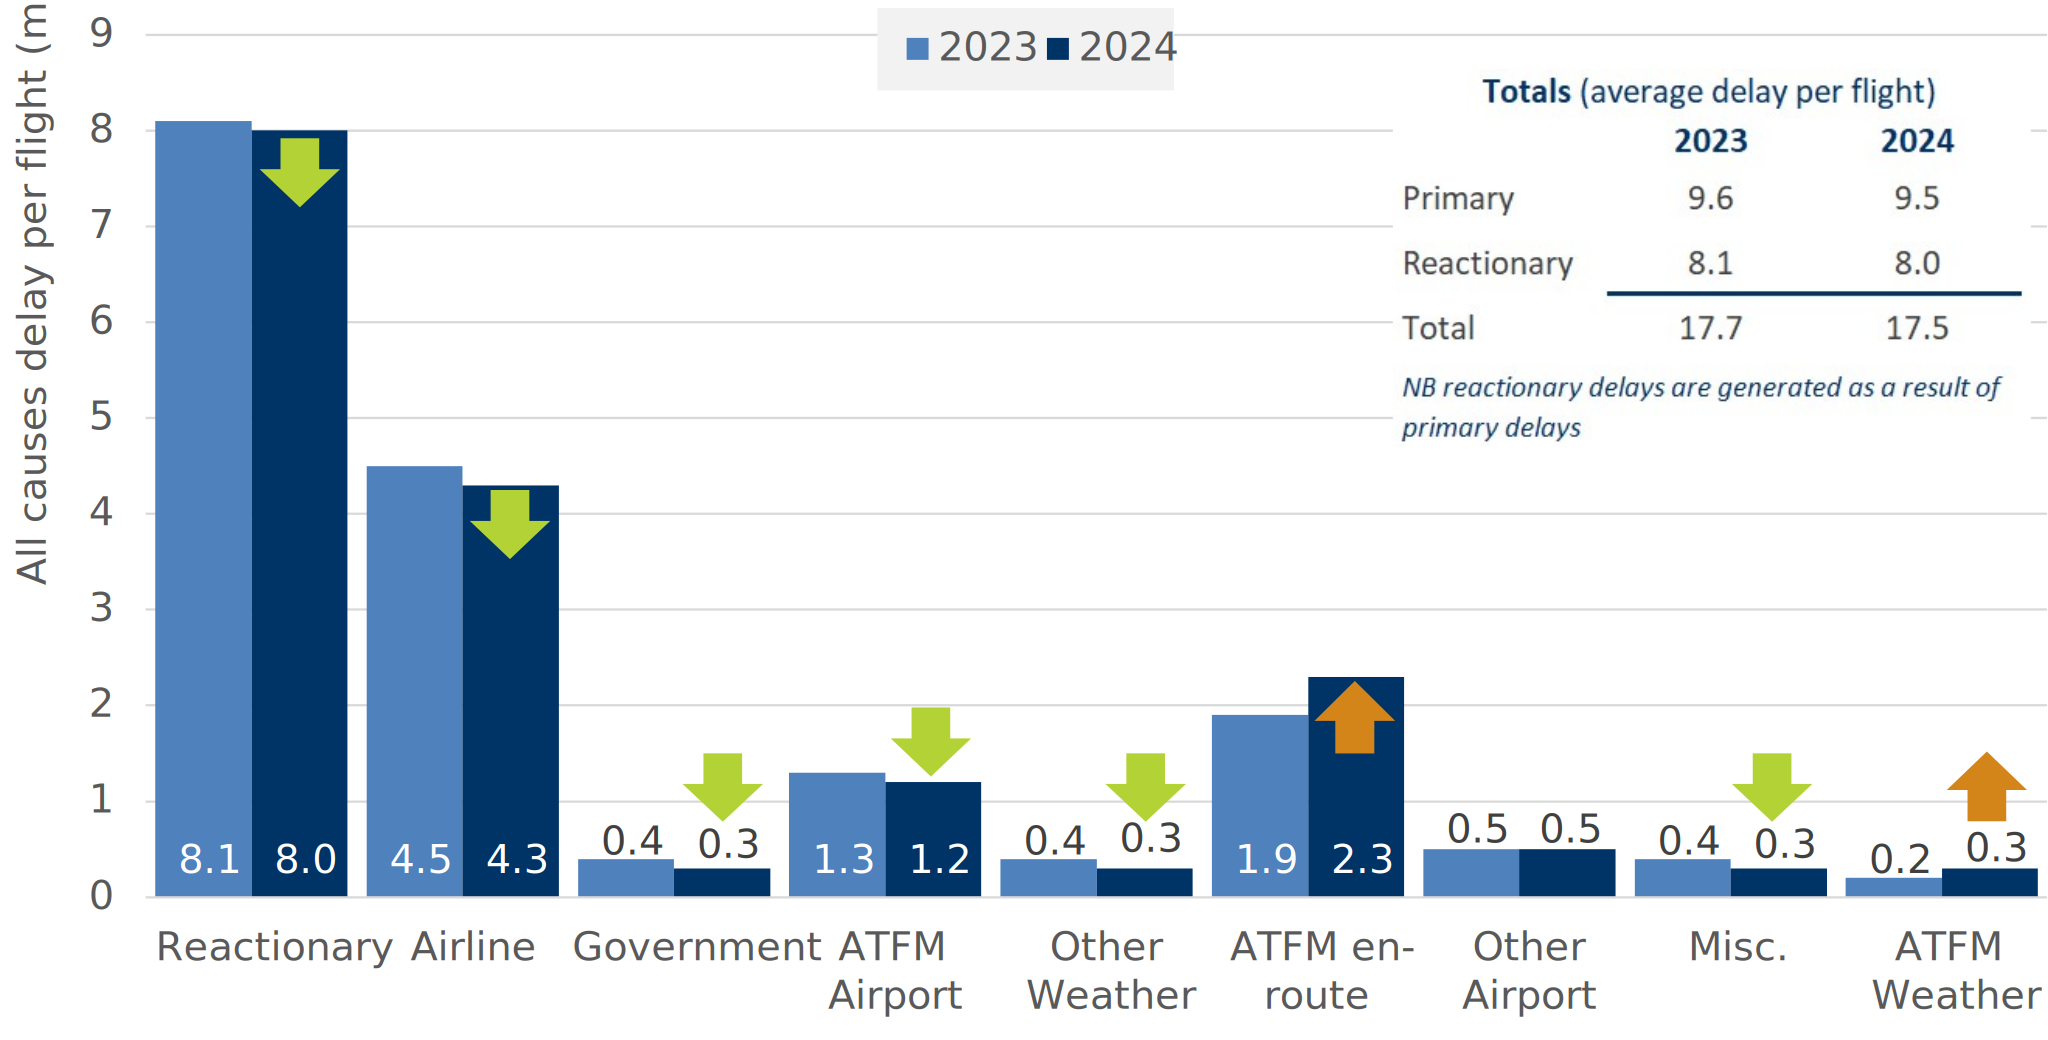
\includegraphics{chapters/../figures/delay_causes.png}

}

\caption{\label{fig-all-causes-delay}Breakdown of the network average
delay per flight on departure: 2021 vs 2020
\protect\hyperlink{ref-coda2021}{{[}14{]}}}

\end{figure}

The ATFM delay constitutes only a fraction of primary delay from all
causes, and around half of all delay is reactionary (i.e., delay caused
by late arrival of aircraft, crew, passengers or baggage from previous
journeys) rather than primary (i.e., delay other than reactionary).

\hypertarget{atfm-delay}{%
\subsection{ATFM delay}\label{atfm-delay}}

Looking specifically into \textbf{ATFM delay},
Figure~\ref{fig-atfm-delay} shows the daily traffic and traffic flow
delay per flight (en-route and at airport) for the period 2012-2021. The
figures presented are calculated by the Network Manager based on the
flight plans and include the planned ATFM delays due to the restrictions
that may be applied in the airspace
\protect\hyperlink{ref-nm2022}{{[}15{]}}.

\begin{figure}

{\centering \includegraphics{chapters/../figures/atfm_delay.png}

}

\caption{\label{fig-atfm-delay}Average daily traffic and ATFM delay per
flight 2012-2022 \protect\hyperlink{ref-nm2022}{{[}15{]}}}

\end{figure}

\hypertarget{when-to-use-the-input-1}{%
\section{When to use the input?}\label{when-to-use-the-input-1}}

We recommend using all causes of delay provided by CODA when analysing
the impacts on airlines or on passengers/society (e.g., an airline
upgrading the avionics in their aircraft; airport expansion, etc.). On
the other hand, ATFM delay is recommended to be used when analysing
projects aiming at improving flow management.

Furthermore, since primary delay shows the delay that is due to direct
triggers, it is recommended to be used when analysing updates that would
impact the non-reactionary delays.

\hypertarget{comments}{%
\section{Comments}\label{comments}}

Looking at both figures above, it can be observed that the ATFM delay,
both at the airport and en-route, is higher when looking at the numbers
provided by the airlines rather than that observed by the Network
Manager. This occurs because the delay numbers provided by the Network
Manager account for the so-called planned delay due to restrictions in
the airspace, while the numbers provided by the airlines cover the total
delay they attribute to ATFM, whether they come from the restrictions or
any other planned ATFM delays

Another important point to take into consideration when analysing the
recommended values is the impact of COVID-19 pandemic. Both, the
all-causes delay and the ATFM delay were impacted by the significant
reduction in air traffic in 2020 and 2021, resulting in a strong drop in
the total delay duration. Thus, when looking into these numbers it is
equally important to consider the situation prior to 2020. For the
All-causes delay this information can be found in the previous editions
of CODA Digest, available in EUROCONTROL library
\protect\hyperlink{ref-ectllibrary}{{[}16{]}}.

\hypertarget{related-inputs-3}{%
\section{Related inputs}\label{related-inputs-3}}

Chapter~\ref{sec-air-traffic-statistics-and-forecasts}
\protect\hyperlink{sec-air-traffic-statistics-and-forecasts}{Air traffic
statistics and forecast}

Chapter~\ref{sec-cost-of-delay}
\protect\hyperlink{sec-cost-of-delay}{Cost of delay}

\hypertarget{references-4}{%
\section{References}\label{references-4}}

\hypertarget{sec-transit-time}{%
\chapter{Transit time}\label{sec-transit-time}}

\hypertarget{eurocontrol-recommended-values-2}{%
\section{EUROCONTROL Recommended
Values}\label{eurocontrol-recommended-values-2}}

The transit time in an ANSP represents the \textbf{average time flown by
aircraft controlled in this airspace over a year}.
Table~\ref{tbl-transit-time} provides an overview of the average transit
time (expressed in minutes) per ANSP in 2019.

The data that was used to build this table, as well as more recent data,
can be accessed on AIU
portal.\protect\hyperlink{ref-aiuportal}{{[}17{]}}

\hypertarget{tbl-transit-time}{}
\setlength{\LTpost}{0mm}
\begin{longtable}{llr}
\caption{\label{tbl-transit-time}Average transit time per country }\tabularnewline

\toprule
ANSP & State & Transit time (min) \\ 
\midrule
Albcontrol & Albania & 13 \\ 
ANS CR & Czech Republic & 20 \\ 
ANS Finland & Finland & 28 \\ 
ARMATS & Armenia & 16 \\ 
Austro Control & Austria & 19 \\ 
AVINOR (Continental) & Norway & 37 \\ 
BULATSA & Bulgaria & 20 \\ 
Croatia Control & Croatia & 22 \\ 
DCAC Cyprus & Cyprus & 29 \\ 
DFS & Germany & 30 \\ 
DHMI & Türkiye & 59 \\ 
DSNA & France & 45 \\ 
EANS & Estonia & 20 \\ 
ENAIRE & Spain & 46 \\ 
ENAV & Italy & 39 \\ 
HCAA & Greece & 42 \\ 
HungaroControl & Hungary & 17 \\ 
IAA & Ireland & 30 \\ 
LFV & Sweden & 35 \\ 
LGS & Latvia & 18 \\ 
LPS & Slovakia & 12 \\ 
LVNL & Netherlands & 17 \\ 
MATS & Malta & 41 \\ 
M-NAV & North Macedonia & 10 \\ 
MOLDATSA & Republic of Moldova & 14 \\ 
MUAC & NA & 22 \\ 
NATS (Continental) & United Kingdom & 37 \\ 
NAV Portugal (Continental) & Portugal & 40 \\ 
NAVIAIR & Denmark & 20 \\ 
Oro Navigacija & Lithuania & 16 \\ 
PANSA & Poland & 34 \\ 
ROMATSA & Romania & 32 \\ 
SAKAERONAVIGATSIA & Georgia & 22 \\ 
skeyes & Belgium & 11 \\ 
Skyguide & Switzerland & 17 \\ 
Slovenia Control & Slovenia & 11 \\ 
SMATSA & Serbia \& Montenegro & 23 \\ 
UkSATSE & Ukraine & 39 \\ 
\bottomrule
\end{longtable}
\begin{minipage}{\linewidth}
\emph{Source: \href{https://ansperformance.eu/data/}{EUROCONTROL Aviation Intelligence Unit}}\\
\end{minipage}

\hypertarget{description}{%
\section{Description}\label{description}}

This metric is the ratio between the total flight hours controlled and
the IFR flights controlled, where:

\begin{itemize}
\item
  Total IFR flight-hours controlled is the sum of the flight-hours
  controlled over the year by the ANSP. For a given flight the
  flight-hours controlled are computed using information available in
  the Network Manager database as the difference between the exit time
  and the entry time in the controlled airspace
\item
  • IFR movements controlled is the number of flights that have been
  controlled over the year by the ANSP
\end{itemize}

In Figure~\ref{fig-transit-time}, the range of transit time values for
the vast majority of ANSPs in Europe can be observed (Note: the scope is
limited to the 38 ANSPs reporting to the
\href{https://ansperformance.eu/about/prc/}{Performance Review
Commission}). The European average in terms of flight time is 31 minutes
per ANSP. A difference of 49 minutes between the highest (DHMI Türkiye)
and the lowest (M-NAV North Macedonia) transit time can also be observed
-- this represents a ratio of almost 6 or a Standard Deviation of around
12.

\begin{figure}

{\centering 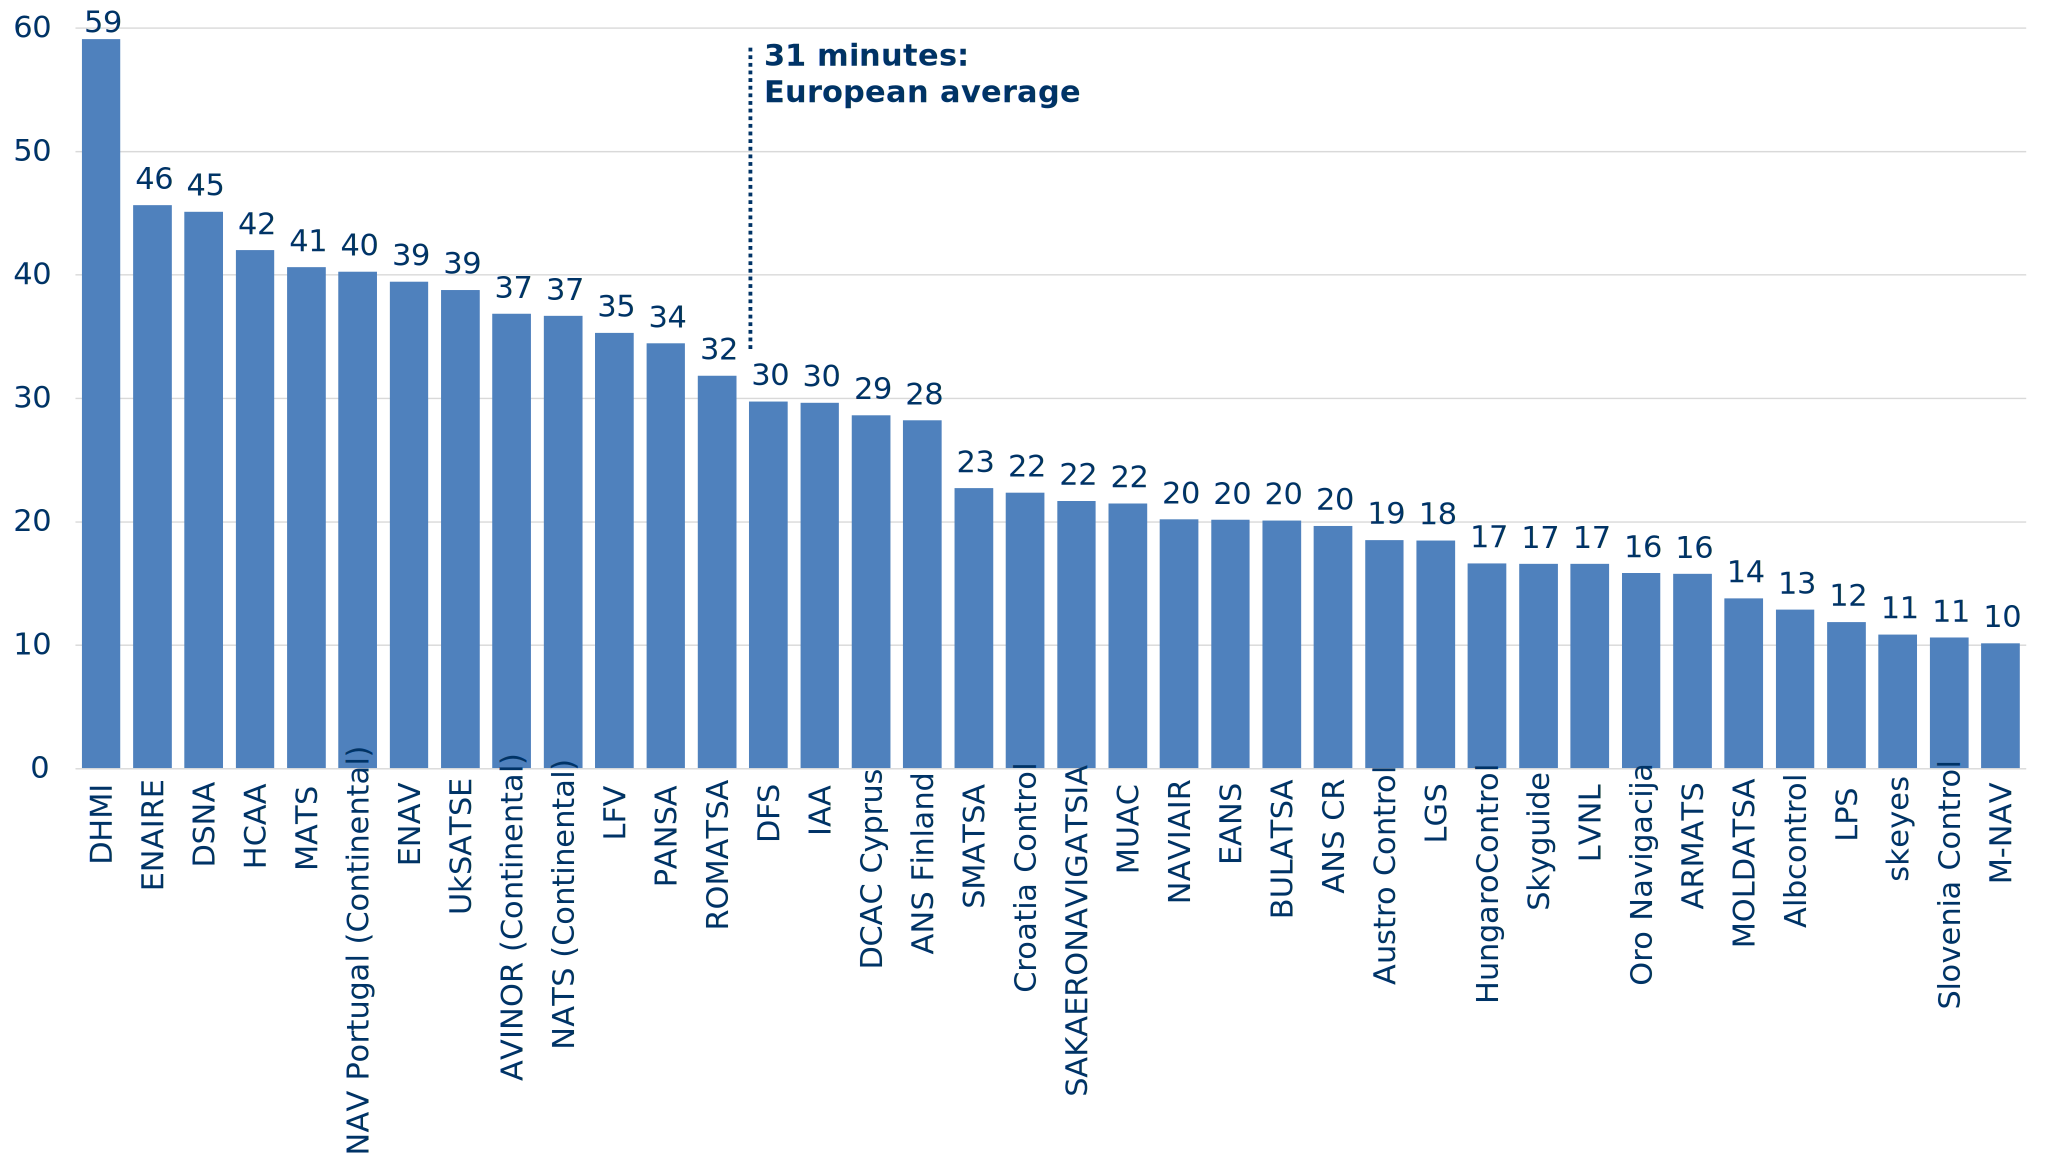
\includegraphics{chapters/../figures/transit_time.svg}

}

\caption{\label{fig-transit-time}Average transit time per country in
2019. \emph{Source: EUROCONTROL}}

\end{figure}

\hypertarget{when-to-use-the-input-2}{%
\section{When to use the input?}\label{when-to-use-the-input-2}}

This input is recommended for those projects where the flying time in a
giver country or a set of countries is key to the assessment. As an
example, it has previously been used for several CNS related studies, in
particular when studying the cost of communication services that depend
on connection times.

\hypertarget{comments-1}{%
\section{Comments}\label{comments-1}}

The data was recorded by the Network Manager (NM) for the 38 ANSPs that
were part of the ACE Report in 2019
\protect\hyperlink{ref-ace2019}{{[}18{]}}. For a few ANSPs, the data
reported show slight differences with the NM records, as ANSPs tend to
communicate their own traffic data. The differences are explained by the
different counting methodology in IFR airport movements for training
flights.

\hypertarget{related-inputs-4}{%
\section{Related inputs}\label{related-inputs-4}}

Chapter~\ref{sec-medium-term-capacity-planning}
\protect\hyperlink{sec-medium-term-capacity-planning}{Medium-term
capacity planning}

\hypertarget{references-5}{%
\section{References}\label{references-5}}

\part{Environment}

\hypertarget{sec-rate-of-fuel-burn}{%
\chapter{Rate of fuel burn}\label{sec-rate-of-fuel-burn}}

\hypertarget{eurocontrol-recommended-values-3}{%
\section{EUROCONTROL recommended
values}\label{eurocontrol-recommended-values-3}}

This section provides the average number of kilogrames per minute of
fuel burn by operator segments in different flight phases.

\hypertarget{tbl-rate-fuel-burn}{}
\setlength{\LTpost}{0mm}
\begin{longtable}{lrrr}
\caption{\label{tbl-rate-fuel-burn}Average fuel burn rates (kg/minute) }\tabularnewline

\toprule
Flight phase & Taxi & En route & Arrival Management \\ 
\midrule
Scheduled aviation & 12.7 & 51.6 & 38.6 \\ 
Regional aircraft & 8.2 & 24.6 & 19.9 \\ 
Narrow body aircraft & 11.7 & 40.1 & 35.2 \\ 
Wide body aircraft & 25.8 & 113.9 & 85.2 \\ 
Business aviation & NA & 9.3 & 7.7 \\ 
Rotorcraft & NA & 8.8 & 8.8 \\ 
\bottomrule
\end{longtable}
\begin{minipage}{\linewidth}
Based on EUROCONTROL \href{https://www.eurocontrol.int/model/bada}{BADA} and \href{https://ansperformance.eu/acronym/prisme/}{PRISME} data\\
\end{minipage}

\hypertarget{description-1}{%
\section{Description}\label{description-1}}

Table~\ref{tbl-rate-fuel-burn} originates from the Base of Aircraft Data
(BADA), an Aircraft Performance Model (APM) developed and maintained by
EUROCONTROL, with the active cooperation of aircraft manufacturers and
operating airlines. The data extracted use three different families of
the BADA model (BADA 3, BADA 4, and BADA Helicopters).

The operating segment values are weighted averages calculated based on
(i) the number of flights per aircraft type (taxi and arrival phases) or
(ii) the number of flight hours per aircraft type (en-route phase). The
analysis covers the most-flying aircraft models in Europe, as per the
flight plans submitted to the Network Manager (NM) in 2022 (EUROCONTROL
PRISME):

\begin{itemize}
\item
  \textbf{Scheduled aviation}: Grouping three (3) categories from the
  EUROCONTROL Market Segment Rules
  \protect\hyperlink{ref-ectl:market:seg:2022}{{[}12{]}}:

  \begin{itemize}
  \item
    \textbf{Regional (top 5):} AT76, E190, E195, CRJ9, and AT75.
  \item
    \textbf{Mainline + Low cost (top 15):} (a) narrow-body aircraft
    (B738, A320, A319, A20N, A321, A21N, B38M, BCS3, B734) and (b)
    wide-body aircraft (B77W, B789, A333, A332, B788, A359).
  \end{itemize}
\item
  \textbf{Business aviation (top 5):} C56X, PC12, BE20, E55P, and GLEX.
\item
  \textbf{Rotorcraft (top 5):} S92, A139, EC75, AS32, and EC35.
\end{itemize}

The above selection of aircraft covers (i) 76\% of the IFR flights and
(ii) 79\% of the IFR flight hours registered by the NM in 2022.

\hypertarget{when-to-use-the-values}{%
\section{When to use the values?}\label{when-to-use-the-values}}

The user should treat the Table~\ref{tbl-rate-fuel-burn} values as
high-level approximations of the average fuel burn per flight phase.
Note that:

\begin{enumerate}
\def\labelenumi{\roman{enumi})}
\item
  regional and business aviation groupings encompass turbofan-powered
  and turboprop-powered aircraft with fuel burn rates significantly
  different between them;
\item
  the performance data do not consider the weather and atmospheric
  influences; and
\item
  the performance data do not consider the impact of specific flight
  conditions (speed, altitude, aircraft weight, etc.).
\end{enumerate}

Organisations interested in more aircraft types can request access to
the full BADA model.

\hypertarget{other-possible-sources}{%
\section{Other possible sources}\label{other-possible-sources}}

Below, a list of other applicable sources that consider fuel burn rates:

\begin{itemize}
\item
  \emph{ICAO Carbon Emissions Calculator:}
  \protect\hyperlink{ref-emissionscalc}{{[}19{]}} ICAO has developed a
  methodology to calculate the carbon dioxide emissions from air travel
  for use in offset programmes. The methodology applies the best
  publicly available industry data to account for various factors such
  as aircraft types, route-specific data, passenger load factors and
  cargo carried.
\item
  \emph{EUROCONTROL Advanced Emission Model (AEM):}
  \protect\hyperlink{ref-ectrl:em:model}{{[}20{]}} Standalone
  application, developed and maintained by the EUROCONTROL Innovation
  Hub, which estimates aircraft emissions and fuel burn. The AEM can
  estimate (i) the mass of fuel burned by the main engines of a
  specified type of aircraft with a specified type of engine flying a
  specified 4D trajectory; and (ii) the corresponding masses of certain
  gaseous and particulate emissions which are produced by the burning of
  that fuel. Access to the tool requires an AEM user license.
\item
  \emph{ICAO Engine Emissions Databank:}
  \protect\hyperlink{ref-icao:databank}{{[}21{]}} Manufacturer's
  datasheets that may contain the rates of fuel burn for different
  flight phases and individual engine types.
\end{itemize}

\hypertarget{related-inputs-5}{%
\section{Related inputs}\label{related-inputs-5}}

Chapter~\ref{sec-fleet-size} \protect\hyperlink{sec-fleet-size}{Fleet
size}

\hypertarget{references-6}{%
\section{References}\label{references-6}}

\hypertarget{sec-amount-of-emissions-released-by-fuel-burn}{%
\chapter{Amount of emissions released by fuel
burn}\label{sec-amount-of-emissions-released-by-fuel-burn}}

\hypertarget{eurocontrol-recommended-values-4}{%
\section{EUROCONTROL recommended
values}\label{eurocontrol-recommended-values-4}}

This input represents the amount of emissions produced by combustion of
aviation fuel, focusing on the main types of pollutants.

\hypertarget{tbl-emissions-per-kg-fuel}{}
\setlength{\LTpost}{0mm}
\begin{longtable}{lr}
\caption{\label{tbl-emissions-per-kg-fuel}Estimated amount of emissions released per kg of fuel burnt }\tabularnewline

\caption*{
{\large Emissions per kg of fuel burnt} \\ 
{\small fuel = Kerosene}
} \\ 
\toprule
\textbf{Emission type} & \textbf{Emission} \\ 
\midrule
CO2 & 3.15 kg\textsuperscript{a} \\ 
H2O & 1.237 kg\textsuperscript{a} \\ 
SOx & 0.00084 kg\textsuperscript{b} \\ 
 & 0.000114 kg\textsuperscript{c} \\ 
NOx & 0.0148 kg\textsuperscript{d} \\ 
HC & 0.00032 kg\textsuperscript{d} \\ 
CO & 0.00325 kg\textsuperscript{d} \\ 
PM volatile & 0.000092 kg\textsuperscript{d} \\ 
\bottomrule
\end{longtable}
\begin{minipage}{\linewidth}
\textsuperscript{a}Source 1\\
\textsuperscript{b}assuming 440 ppm, Source 2\\
\textsuperscript{c}assuming 600 ppm, Source 2\\
\textsuperscript{d}Source 3\\
\emph{Source 1: \href{https://www.eurocontrol.int/publication/european-aviation-fuel-burn-and-emissions-inventory-system-feis-european-environment}{EUROCONTROL (2018) European Aviation Fuel Burn and Emissions Inventory System for the European Environment Agency}}\\
\emph{Source 2: \href{https://citeseerx.ist.psu.edu/viewdoc/download?doi=10.1.1.719.2090\&rep=rep1\&type=pdf}{MIT (2010) Laboratory for aviation and the environment -- Guidance on the use of AEDT for gridded aircraft emissions in atmospheric models}}\\
\emph{Source 3: \href{https://www.eurocontrol.int/publication/european-aviation-environmental-report-2022}{EUROCONTROL, EASA, EU (2022) European Aviation Environmental Report, EU27+FTA aviation emissions for year 2021}}\\
\end{minipage}

\hypertarget{when-to-use-the-input-3}{%
\section{When to use the input?}\label{when-to-use-the-input-3}}

This input is recommended for a wide use in assessments that focus on
the assessment of environmental impact from the burning of fuel at any
stage of the flight.

\hypertarget{comments-2}{%
\section{Comments}\label{comments-2}}

The Committee on Aviation Environmental Protection (CAEP), a technical
committee of the ICAO Council, recommends the use a conversion factor of
\textbf{3.16 g of CO\textsubscript{2} per gram of Jet A.} The 3.16 value
can be found in ICAO Doc 9889, 1st edition, 2011, and other documents.

However, in Europe, as early as 2009, Commission Decision 2009/339/EC
indicated an emission \textbf{factor of 3.15 for the mass conversion
from Jet A to CO\textsubscript{2}} for the period after January 2021.

In view of the above, emission factor 3.15 should continue to be used in
SESAR 2020, for the sake of internal consistency within the programme,
unless the EU ETS decides to move to 3.16. Factor 3.16 should be used
when the evaluation concerns comparisons with studies carried out within
the ICAO framework or using the factor recommended by ICAO, in order to
ensure external
consistency.\protect\hyperlink{ref-SESAR2020Environment}{{[}22{]}}

\hypertarget{other-possible-sources-1}{%
\section{Other possible sources}\label{other-possible-sources-1}}

\begin{itemize}
\item
  \emph{European Aviation Environmental Report
  Series}\protect\hyperlink{ref-eaer2022}{{[}23{]}} in its latest 2022
  edition shows the aviation sector has taken steps to address
  environmental challenges but also that more decisive actions are
  needed. In particular the latest trends in aircraft engine emissions
  can be checked in section 3.2. of the document.
\item
  \emph{European Environment Agency (2019), EMEP/EEA air pollutant
  emission inventory guidebook
  2019}\protect\hyperlink{ref-eea:2019}{{[}24{]}} provides values for
  emission factors and fuel consumption in different phases of flight --
  including taxiing -- for different aircraft types, using three
  different levels of accuracy and complexity, in section 1.A.3.a of the
  document.
\item
  \textbf{ICAO Aircraft Engine Emissions Databank}, available at
  \href{https://www.easa.europa.eu/en/domains/environment/icao-aircraft-engine-emissions-databank}{EASA
  website} contains information on exhaust emissions of production
  aircraft engines, covering engine types which emissions are regulated,
  namely turbojet and turbofan engines with a static thrust greater than
  26.7 kilonewtons.
\item
  \emph{Swiss Federal Office of Civil Aviation, Aircraft Engine
  Emissions}\protect\hyperlink{ref-foca:aee}{{[}25{]}} presents a
  measurement and calculation methodology for aircraft piston engine
  emissions in order to improve aviation emission inventories, as
  developed by FOCA.
\item
  \emph{Swedish Defence Research
  Agency}\protect\hyperlink{ref-envimpact}{{[}26{]}} holds a database of
  emission indices of NOx, HC and CO, with corresponding fuel flows for
  turboprop engines.
\end{itemize}

\hypertarget{related-inputs-6}{%
\section{Related inputs}\label{related-inputs-6}}

Chapter~\ref{sec-rate-of-fuel-burn}
\protect\hyperlink{sec-rate-of-fuel-burn}{Rate of fuel burn}

Chapter~\ref{sec-cost-of-emissions}
\protect\hyperlink{sec-cost-of-emissions}{Cost of emissions}

Chapter~\ref{sec-ifr-flight-information-per-market-segment}
\protect\hyperlink{sec-ifr-flight-information-per-market-segment}{IFR
flight information per market segment}

\hypertarget{references-7}{%
\section{References}\label{references-7}}

\hypertarget{sec-cost-of-emissions}{%
\chapter{Cost of emissions}\label{sec-cost-of-emissions}}

\hypertarget{eurocontrol-recommended-values-5}{%
\section{EUROCONTROL recommended
values}\label{eurocontrol-recommended-values-5}}

The data provided in the following sub-sections shows an estimation of
the cost of CO\textsubscript{2} and other aircraft pollutants released
by the combustion of aviation fuel.

\hypertarget{air-pollution}{%
\subsection{Air pollution}\label{air-pollution}}

According to the Handbook on the external costs of
transport,\protect\hyperlink{ref-ecdgmove2019}{{[}27{]}} for air
pollution costs, the marginal costs are virtually equal to the average
costs. This is due to the fact that the dose-response relationships
between the emissions of air pollutants and health effects are nearly
linear.

\hypertarget{tbl-marginal-pollution-cost}{}
\setlength{\LTpost}{0mm}
\begin{longtable}{lllrrr}
\caption{\label{tbl-marginal-pollution-cost}Marginal air pollution costs of aviation }\tabularnewline

\toprule
Distance (km) & Emissions class & Example of aircraft type & Cost per LTO\textsuperscript{1} & Cost per pax km (€-cent)\textsuperscript{1} & Cost per pax\textsuperscript{1} \\ 
\midrule
\multicolumn{6}{l}{Short-haul} \\ 
\midrule
$500$ & Low & Bombardier CRJ900 & $\text{EUR}120.00$ & $\text{EUR}0.33$ & $\text{EUR}1.68$ \\ 
$500$ & High & Embraer 170 & $\text{EUR}162.00$ & $\text{EUR}0.36$ & $\text{EUR}1.80$ \\ 
\midrule
\multicolumn{6}{l}{Medium-haul} \\ 
\midrule
$1,500$ & Low & Airbus 320 & $\text{EUR}196.00$ & $\text{EUR}0.08$ & $\text{EUR}1.32$ \\ 
$1,500$ & High & Boeing 737 & $\text{EUR}219.00$ & $\text{EUR}0.13$ & $\text{EUR}1.87$ \\ 
$3,000$ & Low & Airbus 320 & $\text{EUR}260.00$ & $\text{EUR}0.06$ & $\text{EUR}1.74$ \\ 
$3,000$ & High & Boeing 737 & $\text{EUR}290.00$ & $\text{EUR}0.08$ & $\text{EUR}2.48$ \\ 
\midrule
\multicolumn{6}{l}{Long-haul} \\ 
\midrule
$5,000$ & Low & Airbus 340 & $\text{EUR}595.00$ & $\text{EUR}0.04$ & $\text{EUR}2.01$ \\ 
$5,000$ & High & Boeing 777 & $\text{EUR}987.00$ & $\text{EUR}0.05$ & $\text{EUR}2.28$ \\ 
$15,000$ & Low & Airbus 340 & $\text{EUR}843.00$ & $\text{EUR}0.02$ & $\text{EUR}2.86$ \\ 
$15,000$ & High & Boeing 777 & $\text{EUR}1,397.00$ & $\text{EUR}0.02$ & $\text{EUR}3.22$ \\ 
\bottomrule
\end{longtable}
\begin{minipage}{\linewidth}
\textsuperscript{1}The monetary values are adjusted to 2022 prices according to inflation\\
\emph{Source: \href{https://data.europa.eu/doi/10.2832/51388}{European Commission (2019), Handbook on the external costs of transport}}\\
\end{minipage}

\hypertarget{climate-change}{%
\subsection{Climate change}\label{climate-change}}

One of the approaches to monetise the climate change costs is to
estimate the CO\textsubscript{2} cost avoidance, in compliance with the
provisions of Paris Climate Agreement.
Table~\ref{tbl-climate-change-cost} provides an estimate of
CO\textsubscript{2} equivalent cost avoidance for short and medium term.
It shows a low, medium and high estimate of these values.

\hypertarget{tbl-climate-change-cost}{}
\setlength{\LTpost}{0mm}
\begin{longtable}{lrrr}
\caption{\label{tbl-climate-change-cost}Climate change avoidance costs in € per tonne of CO2 equivalent }\tabularnewline

\toprule
  & Low\textsuperscript{1} & Medium\textsuperscript{1} & High\textsuperscript{1} \\ 
\midrule
Short and medium run (up to 2030) & $\text{EUR}71.00$ & $\text{EUR}119.00$ & $\text{EUR}224.00$ \\ 
Long run (from 2040 to 2060) & $\text{EUR}185.00$ & $\text{EUR}319.00$ & $\text{EUR}590.00$ \\ 
\bottomrule
\end{longtable}
\begin{minipage}{\linewidth}
\textsuperscript{1}The values are adjusted to 2022 prices according to inflation\\
\emph{Source: \href{https://data.europa.eu/doi/10.2832/51388}{European Commission (2019), Handbook on the external costs of transport}}\\
\end{minipage}

\hypertarget{other-possible-values}{%
\subsection{Other possible values}\label{other-possible-values}}

The well-to-tank emissions costs represent the costs linked to the
production of all different type of energy sources, which leads to
emissions and other externalities. It includes the extraction of energy,
processing, transport and transmission, building of energy plants, etc.
These emissions are part of the most relevant emissions when it comes to
transportation.

Table~\ref{tbl-wtt-costs} presents the estimated cost of well-to-tank
emissions from aviation based on an analysis of 33 selected EU airports.

\hypertarget{tbl-wtt-costs}{}
\setlength{\LTpost}{0mm}
\begin{longtable}{lrrr}
\caption{\label{tbl-wtt-costs}Total and average well-to-tank costs for aviation for 33 selected EU
airports }\tabularnewline

\toprule
  & Total cost (bn €)\textsuperscript{1} & €-cents per pkm\textsuperscript{1} & €-cents per pax\textsuperscript{1} \\ 
\midrule
Short-haul (< 1,500 km) & $\text{EUR}1.10$ & $\text{EUR}1.20$ & $\text{EUR}6.60$ \\ 
Medium-haul (1,500 km > 5,000 km) & $\text{EUR}2.40$ & $\text{EUR}0.80$ & $\text{EUR}14.40$ \\ 
Long-haul (> 5,000 km) & $\text{EUR}6.60$ & $\text{EUR}1.00$ & $\text{EUR}80.60$ \\ 
\bottomrule
\end{longtable}
\begin{minipage}{\linewidth}
\textsuperscript{1}The values are adjusted to 2022 prices according to inflation\\
\emph{Source: \href{https://data.europa.eu/doi/10.2832/51388}{European Commission (2019), Handbook on the external costs of transport}}\\
\end{minipage}

Table~\ref{tbl-wtt-pollution} presents the damage cost factors used for
calculation of the emissions impacts. The prices are expressed in € per
kg and were adjusted to 2022 prices from 2016.

\hypertarget{tbl-wtt-pollution}{}
\setlength{\LTpost}{0mm}
\begin{longtable}{lrrrr}
\caption{\label{tbl-wtt-pollution}Well-to-tank air pollution costs. Damage cost estimates for EU27+UK }\tabularnewline

\toprule
  & NOx & NMVOC & SO2 & PM2.5 (exhaust) \\ 
\midrule
EU27+UK & $\text{EUR}12.90$ & $\text{EUR}1.40$ & $\text{EUR}12.90$ & $\text{EUR}23.00$ \\ 
\bottomrule
\end{longtable}
\begin{minipage}{\linewidth}
\emph{Source: \href{https://data.europa.eu/doi/10.2832/51388}{European Commission (2019), Handbook on the external costs of transport}}\\
\end{minipage}

\hypertarget{further-reading}{%
\section{Further reading}\label{further-reading}}

Below are listed some sources that may be interesting to consult in the
frame of this topic:

\begin{itemize}
\item
  \emph{EUROCONTROL (2022), European Environmental Report}
  \protect\hyperlink{ref-eaer2022}{{[}23{]}}
\item
  \emph{European Commission Climate Action}
  \protect\hyperlink{ref-ecc:limateaction}{{[}28{]}}
\item
  \emph{UK Department for Environment, Food and Rural Affairs (DEFRA)
  (2020), Air quality damage cost update 2020}
  \protect\hyperlink{ref-defra:2020}{{[}29{]}}
\end{itemize}

\hypertarget{related-inputs-7}{%
\section{Related inputs}\label{related-inputs-7}}

Chapter~\ref{sec-rate-of-fuel-burn}
\protect\hyperlink{ec-rate-of-fuel-burn}{Rate of fuel burn}

Chapter~\ref{sec-amount-of-emissions-released-by-fuel-burn}
\protect\hyperlink{sec-amount-of-emissions-released-by-fuel-burn}{Amount
of emissions released by fuel burn}

\hypertarget{references-8}{%
\section{References}\label{references-8}}

\hypertarget{sec-cost-of-noise}{%
\chapter{Cost of noise}\label{sec-cost-of-noise}}

\hypertarget{eurocontrol-recommended-values-6}{%
\section{EUROCONTROL recommended
values}\label{eurocontrol-recommended-values-6}}

The figures hereafter provide values recommended to be used to estimate
the cost of noise per person affected, taking into account the cost of
annoyance as well as the health costs due to exposure to air traffic
noise.

Table~\ref{tbl-yearly-noise-cost} provides an \textbf{estimation of the
average cost of annoyance for the population, health-related costs, as
well as a total (i.e.~annoyance and health) from aviation traffic noise
for EU27+UK.}\protect\hyperlink{ref-ecdgmove2019}{{[}27{]}}

Annoyance refers to the disturbance which individuals experience when
they are exposed to noise (e.g.~discomfort, inconvenience, etc.).

Health impacts are those caused by long-term exposure to noise, such as
stress-related health problems. Evidence has not been strong for all
noise-related health impacts, and consequently in the European Handbook
on External Costs of Transport, only the following health impacts are
considered: hypertension, ischaemic heart disease, stroke and dementia.
Insomnia is not included in order to avoid double-counting with the
costs of annoyance.

The data is presented for different noise levels and the values in euros
represent cost per person and dB.

\hypertarget{tbl-yearly-noise-cost}{}
\setlength{\LTpost}{0mm}
\begin{longtable}{lrrr}
\caption{\label{tbl-yearly-noise-cost}Yearly environmental cost of aviation traffic noise for the EU27+UK }\tabularnewline

\toprule
Noise level (Lden in dB(A))\textsuperscript{1,2} & Annoyance\textsuperscript{3} & Health\textsuperscript{3} & Total\textsuperscript{3} \\ 
\midrule
50‑54 & $\text{EUR}40.00$ & $\text{EUR}6.00$ & $\text{EUR}46.00$ \\ 
55‑59 & $\text{EUR}81.00$ & $\text{EUR}7.00$ & $\text{EUR}88.00$ \\ 
60‑64 & $\text{EUR}81.00$ & $\text{EUR}11.00$ & $\text{EUR}91.00$ \\ 
65‑69 & $\text{EUR}153.00$ & $\text{EUR}14.00$ & $\text{EUR}167.00$ \\ 
70‑74 & $\text{EUR}153.00$ & $\text{EUR}19.00$ & $\text{EUR}172.00$ \\ 
≥ 75 & $\text{EUR}153.00$ & $\text{EUR}25.00$ & $\text{EUR}178.00$ \\ 
\bottomrule
\end{longtable}
\begin{minipage}{\linewidth}
\textsuperscript{1}Lden is the common EU indicator which corresponds to the average noise level throughout the day, evening and night to which a citizen is exposed over a year. One fundamental feature of Lden is that it assumes that evening and night-time noise is more of a nuisance than daytime noise.     (Evening noise is given a penalty of 5 dB(A). Night-time noise is given a penalty of 10 dB(A).)\\
\textsuperscript{2}The basic measurement index for noise is the decibel (dB). It is indexed logarithmically, reflecting the logarithmic manner in which the human ear responds to sound pressure. Within the human range of hearing, deep and very high tones at the same sound intensity are experienced as less noisy. To correct for this sensitivity, a frequency weighting is applied to measurements and calculations.  The most common frequency weighting is the ‘A weighting’, dB(A).\\
\textsuperscript{3}The monetary values are adjusted from 2016 to 2022 prices\\
\emph{Source: \href{https://op.europa.eu/en/publication-detail/-/publication/9781f65f-8448-11ea-bf12-01aa75ed71a1}{European Commission, Directorate-General for Mobility and Transport, Essen, H., Fiorello, D., El Beyrouty, K., et al., Handbook on the external costs of transport: version 2019 -- 1.1, Publications Office, 2020}}\\
\end{minipage}

Table~\ref{tbl-total-noise-cost} presents an assessment of the costs of
noise for short, medium and long-haul flights based on an analysis of 33
EU airports.

\hypertarget{tbl-total-noise-cost}{}
\setlength{\LTpost}{0mm}
\begin{longtable}{lrrrrr}
\caption{\label{tbl-total-noise-cost}Total and average cost of noise cost for aviation at airports }\tabularnewline

\toprule
  & Bn €\textsuperscript{1} & € per LTO\textsuperscript{1} & € per pax\textsuperscript{2,1} & € per tonne\textsuperscript{1} & € per km\textsuperscript{1} \\ 
\midrule
Short-haul (< 1,500 km) & $\text{EUR}1.00$ & $\text{EUR}305.00$ & $\text{EUR}2.43$ & $\text{EUR}10.71$ & $\text{EUR}0.55$ \\ 
Medium-haul (1,500 km > 5,000 km) & $\text{EUR}1.00$ & $\text{EUR}305.00$ & $\text{EUR}2.43$ & $\text{EUR}10.71$ & $\text{EUR}0.33$ \\ 
Long-haul (> 5,000 km) & $\text{EUR}1.00$ & $\text{EUR}305.00$ & $\text{EUR}2.43$ & $\text{EUR}10.71$ & $\text{EUR}0.01$ \\ 
\bottomrule
\end{longtable}
\begin{minipage}{\linewidth}
\textsuperscript{1}The monetary values are adjusted from 2016 to 2022 prices\\
\textsuperscript{2}Costs per pax include the complete flight (not only the half-way principle).\\
\emph{Source: \href{https://op.europa.eu/en/publication-detail/-/publication/9781f65f-8448-11ea-bf12-01aa75ed71a1}{European Commission, Directorate-General for Mobility and Transport, Essen, H., Fiorello, D., El Beyrouty, K., et al., Handbook on the external costs of transport: version 2019 -- 1.1, Publications Office, 2020}}\\
\end{minipage}

\hypertarget{other-possible-values-1}{%
\section{Other possible values}\label{other-possible-values-1}}

Below are presented the results of an economic valuation tool developed
by the UK Department for Environment, Food and Rural Affairs. It
converts changes in noise exposure to estimated monetary values, in
order to support the assessment of the effects of environmental noise.
It details the current understanding of the links between environmental
noise and various effects, including sleep disturbance, annoyance,
hypertension and related
diseases.\protect\hyperlink{ref-GuidanceNoisePollution}{{[}30{]}}

\hypertarget{tbl-noise-household}{}
\setlength{\LTpost}{0mm}
\begin{longtable}{lrr}
\caption{\label{tbl-noise-household}Yearly aviation noise marginal cost per household }\tabularnewline

\toprule
Increase in daytime noise metric by one decibel (dB) & Aviation noise marginal cost (excl. sleep disturbance)\textsuperscript{1} & Sleep disturbance cost\textsuperscript{1} \\ 
\midrule
45-46 & $\text{EUR}20.00$ & $\text{EUR}48.00$ \\ 
50-51 & $\text{EUR}49.00$ & $\text{EUR}66.00$ \\ 
55-56 & $\text{EUR}62.00$ & $\text{EUR}85.00$ \\ 
60-61 & $\text{EUR}80.00$ & $\text{EUR}103.00$ \\ 
65-66 & $\text{EUR}101.00$ & $\text{EUR}121.00$ \\ 
70-71 & $\text{EUR}123.00$ & $\text{EUR}121.00$ \\ 
75-76 & $\text{EUR}146.00$ & $\text{EUR}121.00$ \\ 
80-81 & $\text{EUR}158.00$ & $\text{EUR}121.00$ \\ 
\bottomrule
\end{longtable}
\begin{minipage}{\linewidth}
\textsuperscript{1}The monetary values are adjusted from 2014 to 2022 prices\\
\emph{Source: \href{https://www.gov.uk/government/uploads/system/uploads/attachment_data/file/380852/environmental-noise-valuing-imapcts-PB14227.pdf}{UK Department for Environment, Food and Rural Affairs (2014) Environmental Noise: Valuing impacts on: sleep disturbance, annoyance, hypertension, productivity and quiet}}\\
\end{minipage}

\hypertarget{references-9}{%
\section{References}\label{references-9}}

\hypertarget{sec-shadow-cost-of-carbon}{%
\chapter{Shadow cost of carbon}\label{sec-shadow-cost-of-carbon}}

\hypertarget{eurocontrol-recommended-values-7}{%
\section{EUROCONTROL recommended
values}\label{eurocontrol-recommended-values-7}}

The shadow cost of carbon is the cost of carbon required to drive the
economy to meet the 1.5°C global temperature target set by the
Intergovernmental Panel on Climate Change (IPCC). The values have been
estimated based on the data provided by the European Investment Bank in
their 2021-2025 roadmap \protect\hyperlink{ref-eib2020}{{[}31{]}} and
represent the cost in euros per tonne of CO\textsubscript{2} equivalent.

The input is an adjustment of the EIB recommended values to reflect the
most realistic cost of meeting the
\href{https://unfccc.int/process-and-meetings/the-paris-agreement/the-paris-agreement}{UN
Paris agreement} to limit global warming well below 2 degrees Celsius,
ideally 1.5 -- compared to pre-industrial levels
\protect\hyperlink{ref-ipcc2018}{{[}32{]}}. Please note this input does
not refer to the traditional \emph{market price} but to the \emph{shadow
cost of carbon}, i.e.~considering externalities and future policies. The
original EIB proposed inputs are expressed in 2016 prices
\protect\hyperlink{ref-eib2020}{{[}31{]}} and have been adjusted to 2021
price levels using the values provided in
Table~\ref{tbl-inflation-table}.

\begin{figure}

{\centering \includegraphics{chapters/../figures/cost_of_carbon.png}

}

\caption{\label{fig-cost-of-carbon}Forecast shadow cost of carbon for
EU27 in 2021 prices}

\end{figure}

\hypertarget{when-to-use-the-input-4}{%
\section{When to use the input?}\label{when-to-use-the-input-4}}

This input is recommended for projects where the full socio-economic
value of the initiative is studied, particularly involving the
environmental assessment.

\hypertarget{comments-3}{%
\section{Comments}\label{comments-3}}

In Economic Analyses the concept of `shadow cost' is often used when
working with an abstract commodity or intangible asset. Typically, two
elements are reflected in the `shadow cost':

\begin{itemize}
\tightlist
\item
  The cost of negative externalities such as pollution in this case
\item
  The shadow cost involves the consideration of future policies
\end{itemize}

Shadow costs are inexact by definition, as they are based on
assumptions, but their usefulness resides in that they help to
understand the full socio-economic merits of a project. Please note that
the shadow cost of carbon does not constitute in any way an optimal
value for any policy instrument.

\hypertarget{related-inputs-8}{%
\section{Related inputs}\label{related-inputs-8}}

Chapter~\ref{sec-rate-of-fuel-burn}
\protect\hyperlink{sec-rate-of-fuel-burn}{Rate of fuel burn}

Chapter~\ref{sec-amount-of-emissions-released-by-fuel-burn}
\protect\hyperlink{sec-amount-of-emissions-released-by-fuel-burn}{Amount
of emissions released by fuel burn}

Chapter~\ref{sec-cost-of-emissions}
\protect\hyperlink{sec-cost-of-emissions}{Cost of emissions}

Chapter~\ref{sec-proportion-of-saf}
\protect\hyperlink{sec-proportion-of-saf}{Proportion of SAF}

\hypertarget{references-10}{%
\section{References}\label{references-10}}

\hypertarget{sec-proportion-of-saf}{%
\chapter{Proportion of sustainable aviation
fuel}\label{sec-proportion-of-saf}}

\hypertarget{eurocontrol-recommended-values-8}{%
\section{EUROCONTROL recommended
values}\label{eurocontrol-recommended-values-8}}

This input represents the expected evolution in the proportion of
Sustainable Aviation Fuel (SAF) in the total fuel blend between 2023 and
2050. The evolution is estimated according to three scenarios:

\begin{itemize}
\item
  \textbf{Base scenario}, where a moderate traffic growth and uptake of
  SAF is assumed, in line with \emph{ReFuelEU Aviation}
  \protect\hyperlink{ref-easa:Fit55ReFuelEU}{{[}33{]}} obligations .
\item
  \textbf{High scenario}, assumed that the high availability of SAF will
  foster the quicker adoption of these fuels than outlined in the
  current regulatory requirements.
\item
  \textbf{Low scenario}, which assumes an uptake of SAF slower that
  outlined by existing regulation.
\end{itemize}

\hypertarget{tbl-saf-blend}{}
\setlength{\LTpost}{0mm}
\begin{longtable}{lccc}
\caption{\label{tbl-saf-blend}Forecast evolution of SAF blend 2023-2050 }\tabularnewline

\toprule
Year & High scenario & Base scenario & Low scenario \\ 
\midrule
$2023$ & $1.4\%$ & $1.0\%$ & $0.8\%$ \\ 
$2024$ & $2.1\%$ & $1.5\%$ & $1.2\%$ \\ 
$2025$ & $2.8\%$ & $2.0\%$ & $1.6\%$ \\ 
$2026$ & $4.2\%$ & $2.6\%$ & $2.1\%$ \\ 
$2027$ & $5.7\%$ & $3.2\%$ & $2.6\%$ \\ 
$2028$ & $7.1\%$ & $3.8\%$ & $3.0\%$ \\ 
$2029$ & $8.6\%$ & $4.4\%$ & $3.5\%$ \\ 
$2030$ & $10.0\%$ & $5.0\%$ & $4.0\%$ \\ 
$2035$ & $29.6\%$ & $20.0\%$ & $16.0\%$ \\ 
$2040$ & $49.1\%$ & $32.0\%$ & $25.6\%$ \\ 
$2045$ & $68.7\%$ & $38.0\%$ & $30.4\%$ \\ 
$2050$ & $88.2\%$ & $63.0\%$ & $50.4\%$ \\ 
\bottomrule
\end{longtable}
\begin{minipage}{\linewidth}
\emph{Source: \href{https://www.eurocontrol.int/publication/objective-skygreen-2022-2030}{EUROCONTROL (2022), Objective Skygreen 2022-2030. The economics of aviation decarbonisation towards the 2030 Green Deal milestone}}\\
\end{minipage}

\hypertarget{description-2}{%
\section{Description}\label{description-2}}

Table~\ref{tbl-saf-blend} shows the forecast SAF blending percentage
over total jet fuel for years 2023 to 2050. The values are provided
based on the 3 forecast scenarios proposed by EUROCONTROL Aviation
Outlook\protect\hyperlink{ref-aviation:outlook2022}{{[}6{]}}.

The percentages of SAF are based on:

\begin{itemize}
\tightlist
\item
  The series starting with a projection of the 2022 actual SAF blending.
\item
  A linear interpolation, until in 2030 the required 5\% of the ReFuelEU
  Aviation proposal is met, followed by the same linear growth until
  2050.
\end{itemize}

Other underlying assumptions worth mentioning are:

\begin{itemize}
\tightlist
\item
  The regulation imposes obligations only on the fuel suppliers, not on
  the airlines.
\item
  Objective Skygreen
  2022-2030\protect\hyperlink{ref-skygreen2022}{{[}34{]}} assumes that
  the SAF blending percentages apply to all the airports within the
  Network Manager area (see Figure~\ref{fig-ecac-airspace-fir}).
\end{itemize}

The figure below depicts the expected SAF blending percentages. Points
are the yearly percentages expected and the dotted line is a trend line
adjustment.

\begin{figure}

{\centering 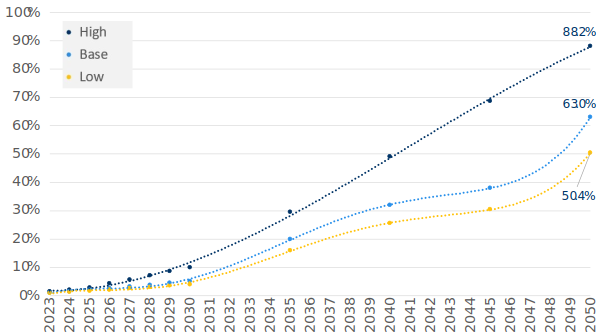
\includegraphics{chapters/../figures/saf_blend.png}

}

\caption{\label{fig-saf-blend}Forecast evolution of SAF proportion
2023-2050\protect\hyperlink{ref-skygreen2022}{{[}34{]}}}

\end{figure}

\hypertarget{when-to-use-the-input-5}{%
\section{When to use the input?}\label{when-to-use-the-input-5}}

This input is recommended to be used when dealing with environmentally
related assessments. This data has previously been used for the traffic
forecast in EUROCONTROL Aviation Outlook 2050
\protect\hyperlink{ref-aviation:outlook2022}{{[}6{]}} and for the
Objective Skygreen study \protect\hyperlink{ref-skygreen2022}{{[}34{]}},
guiding on long-term aviation sustainability.

\hypertarget{comments-4}{%
\section{Comments}\label{comments-4}}

Non-conventional fuels -- SAF are non-fossil derived -- can be used in
aviation if blended with conventional kerosene. Many experts agree that
this is the most promising option to reduce aviation emissions in the
short to medium term.

The ReFuelEU Aviation initiative -- put forward by the European
Commission in the Fit for 55 package -- imposes a mandate on fuel
suppliers to provide SAF in jet fuel available in EU airports. The
proposal defines a series of percentages of SAF blending that will have
to be met at specific years.

For further research, please visit the work of the EUROCONTROL Aviation
Sustainability Unit\protect\hyperlink{ref-ectl:asu}{{[}35{]}}.

\hypertarget{related-inputs-9}{%
\section{Related inputs}\label{related-inputs-9}}

Chapter~\ref{sec-rate-of-fuel-burn}
\protect\hyperlink{sec-rate-of-fuel-burn}{Rate of fuel burn}

Chapter~\ref{sec-amount-of-emissions-released-by-fuel-burn}
\protect\hyperlink{sec-amount-of-emissions-released-by-fuel-burn}{Amount
of emissions released by fuel burn}

Chapter~\ref{sec-cost-of-emissions}
\protect\hyperlink{sec-cost-of-emissions}{Cost of emissions}

Chapter~\ref{sec-shadow-cost-of-carbon}
\protect\hyperlink{sec-shadow-cost-of-carbon}{Shadow cost of carbon}

\hypertarget{references-11}{%
\section{References}\label{references-11}}

\part{Airspace Users}

\hypertarget{sec-aircraft-operating-costs}{%
\chapter{Aircraft operating costs}\label{sec-aircraft-operating-costs}}

\hypertarget{eurocontrol-recommended-values-9}{%
\section{EUROCONTROL recommended
values}\label{eurocontrol-recommended-values-9}}

Table~\ref{tbl-aircraft-operating-cost} presents the flight and ground
costs linked to the operation of an aircraft, such as fuel and oil,
flight deck crew, flight equipment depreciation and amortisation,
aircraft rentals, landing fees, ground handling, aircraft parking, air
bridges and maintenance.

\hypertarget{tbl-aircraft-operating-cost}{}
\setlength{\LTpost}{0mm}
\begin{longtable}{lrrrrr}
\caption{\label{tbl-aircraft-operating-cost}Aircraft Operating Costs in USD 2019 prices }\tabularnewline

\toprule
Aircraft type & per aircraft per year (\$M) & per flight hour & per flight cycle & per available seat km (¢) & per available ton km (¢) \\ 
\midrule
B737 NG & 14.11 & $4,337$ & $9,231$ & 3.76 & 33.11  \\ 
A320 Family & 12.84 & $4,829$ & $8,851$ & 3.60 & 36.92  \\ 
B737 Classic & 8.26 & $2,683$ & $5,366$ & 2.96 & 25.28  \\ 
B777 & 40.01 & $9,507$ & $60,367$ & 3.53 & 22.07  \\ 
A330 & 29.87 & $7,827$ & $35,857$ & 3.61 & 24.48  \\ 
B757 & 18.21 & $5,357$ & $18,508$ & 3.73 & 30.51  \\ 
B767 & 26.00 & $6,675$ & $40,899$ & 3.61 & 22.18  \\ 
B787 & 30.58 & $7,184$ & $50,827$ & 3.11 & 19.86  \\ 
EMB-190 & 10.87 & $4,097$ & $5,770$ & 6.35 & 54.00  \\ 
Dash 8 & 4.03 & $1,921$ & $1,921$ & 6.12 & 58.08  \\ 
\bottomrule
\end{longtable}
\begin{minipage}{\linewidth}
\emph{Source: Values provided by \href{https://www.iata.org/en/services/finance/airline-cost-mgmt/}{IATA Airline Cost Management Group (ACMG)}}\\
\end{minipage}

Figure~\ref{fig-airline-costs-structure} shows the average airline cost
structure for 2019 (considering that jet kerosene price is \$66.9 per
barrel).

\begin{figure}

{\centering \includegraphics{chapters/../figures/Airline_cost_structure.png}

}

\caption{\label{fig-airline-costs-structure}Airline Cost Structure
(2019) \protect\hyperlink{ref-iata:cmg}{{[}36{]}}}

\end{figure}

\hypertarget{description-3}{%
\section{Description}\label{description-3}}

The above values, provided by IATA, refer to the 2020 ACMG data
collection (fiscal year 2019) and provide an overview of the operating
costs for 10 types of aircraft (B737 NG, A320 family, B737 Classic,
B777, A330, B757, B767, B787, EMB-190 and Dash 8). The IATA Airline Cost
Management Group (ACMG) collects operating costs classified into three
categories, which are defined as follows:

\begin{itemize}
\item
  \textbf{Flight operating expenses} are direct operating expenses. They
  are directly related to the aircraft and the flight activities of an
  airline, such as flight crews, fuel, flight equipment and navigation.
  The biggest component of flight operating expenses is fuel and oil at
  48\%.
\item
  \textbf{Ground operating expenses} are also direct operating expenses.
  They are directly related to the ground activities of an airline, such
  as maintenance and overhaul, airport charges, station and ground.
  Maintenance and overhaul is the biggest cost component at 46\%.
\item
  \textbf{System operating expenses} are overheads and indirect
  operating expenses. They are not directly related to flight or ground
  operating expenses. They include costs for cabin attendants, passenger
  service, load insurance, reservations, ticketing, sales and promotion,
  IT and communications, and general and administrative costs, with the
  latter representing 34\% of total system operating expenses.
\end{itemize}

Below, the airline cost structure for each category of expenses (2019):

\begin{figure}

\begin{minipage}[t]{0.50\linewidth}

{\centering 

\begin{figure}

{\centering \includegraphics{chapters/aircraft_operating_costs_files/figure-pdf/fig-total-operating-costs-1.pdf}

}

\caption{Total Operating Costs Structure (2019)}

\end{figure}

}

\end{minipage}%
%
\begin{minipage}[t]{0.50\linewidth}

{\centering 

\begin{figure}

{\centering \includegraphics{chapters/aircraft_operating_costs_files/figure-pdf/fig-flight-operating-costs-1.pdf}

}

\caption{Flight Operating Costs Structure (2019)}

\end{figure}

}

\end{minipage}%
\newline
\begin{minipage}[t]{0.50\linewidth}

{\centering 

\begin{figure}

{\centering \includegraphics{chapters/aircraft_operating_costs_files/figure-pdf/fig-ground-operating-costs-1.pdf}

}

\caption{Ground Operating Costs Structure (2019)}

\end{figure}

}

\end{minipage}%
%
\begin{minipage}[t]{0.50\linewidth}

{\centering 

\begin{figure}

{\centering \includegraphics{chapters/aircraft_operating_costs_files/figure-pdf/fig-system-operating-costs-1.pdf}

}

\caption{System Operating Costs Structure (2019)}

\end{figure}

}

\end{minipage}%

\caption{\label{fig-operating-costs-split}Airline cost structure}

\end{figure}

\hypertarget{data-scope}{%
\section{Data scope}\label{data-scope}}

The values used for analysis are the result of aggregating the cost data
provided by 51 airlines worldwide (\$26.5 billion expenditure), covering
over 35\% of the industry in terms of revenue passenger kilometres
(RPKs), with European airlines representing 16\% of the share and 12\%
in terms of passengers carried.

\hypertarget{data-limitations}{%
\section{Data limitations}\label{data-limitations}}

In a number of jurisdictions, airport charges and taxes that are levied
on a per-passenger basis are not accounted for in airline profit and
loss accounts. As a result, the share of airport charges is likely to be
significantly understated, as airports may levy more on (i) a
per-passenger or (ii) per-aircraft in some jurisdictions. To give an
order of magnitude, in some regions the ACI (Airports Council
International) estimates that over 50\% of airport charges are collected
on a per-passenger basis, reaching as much as 80\% in some regions
worldwide.

\hypertarget{references-12}{%
\section{References}\label{references-12}}

\hypertarget{sec-average-number-of-passengers}{%
\chapter{Average number of
passengers}\label{sec-average-number-of-passengers}}

\hypertarget{eurocontrol-recommended-values-10}{%
\section{EUROCONTROL recommended
values}\label{eurocontrol-recommended-values-10}}

Figure~\ref{fig-number-of-passengers} presents an overview of the total
and average number of passengers per flight in ECAC
\protect\hyperlink{ref-ectrl:statfor:sid}{{[}5{]}}.

\begin{figure}

{\centering 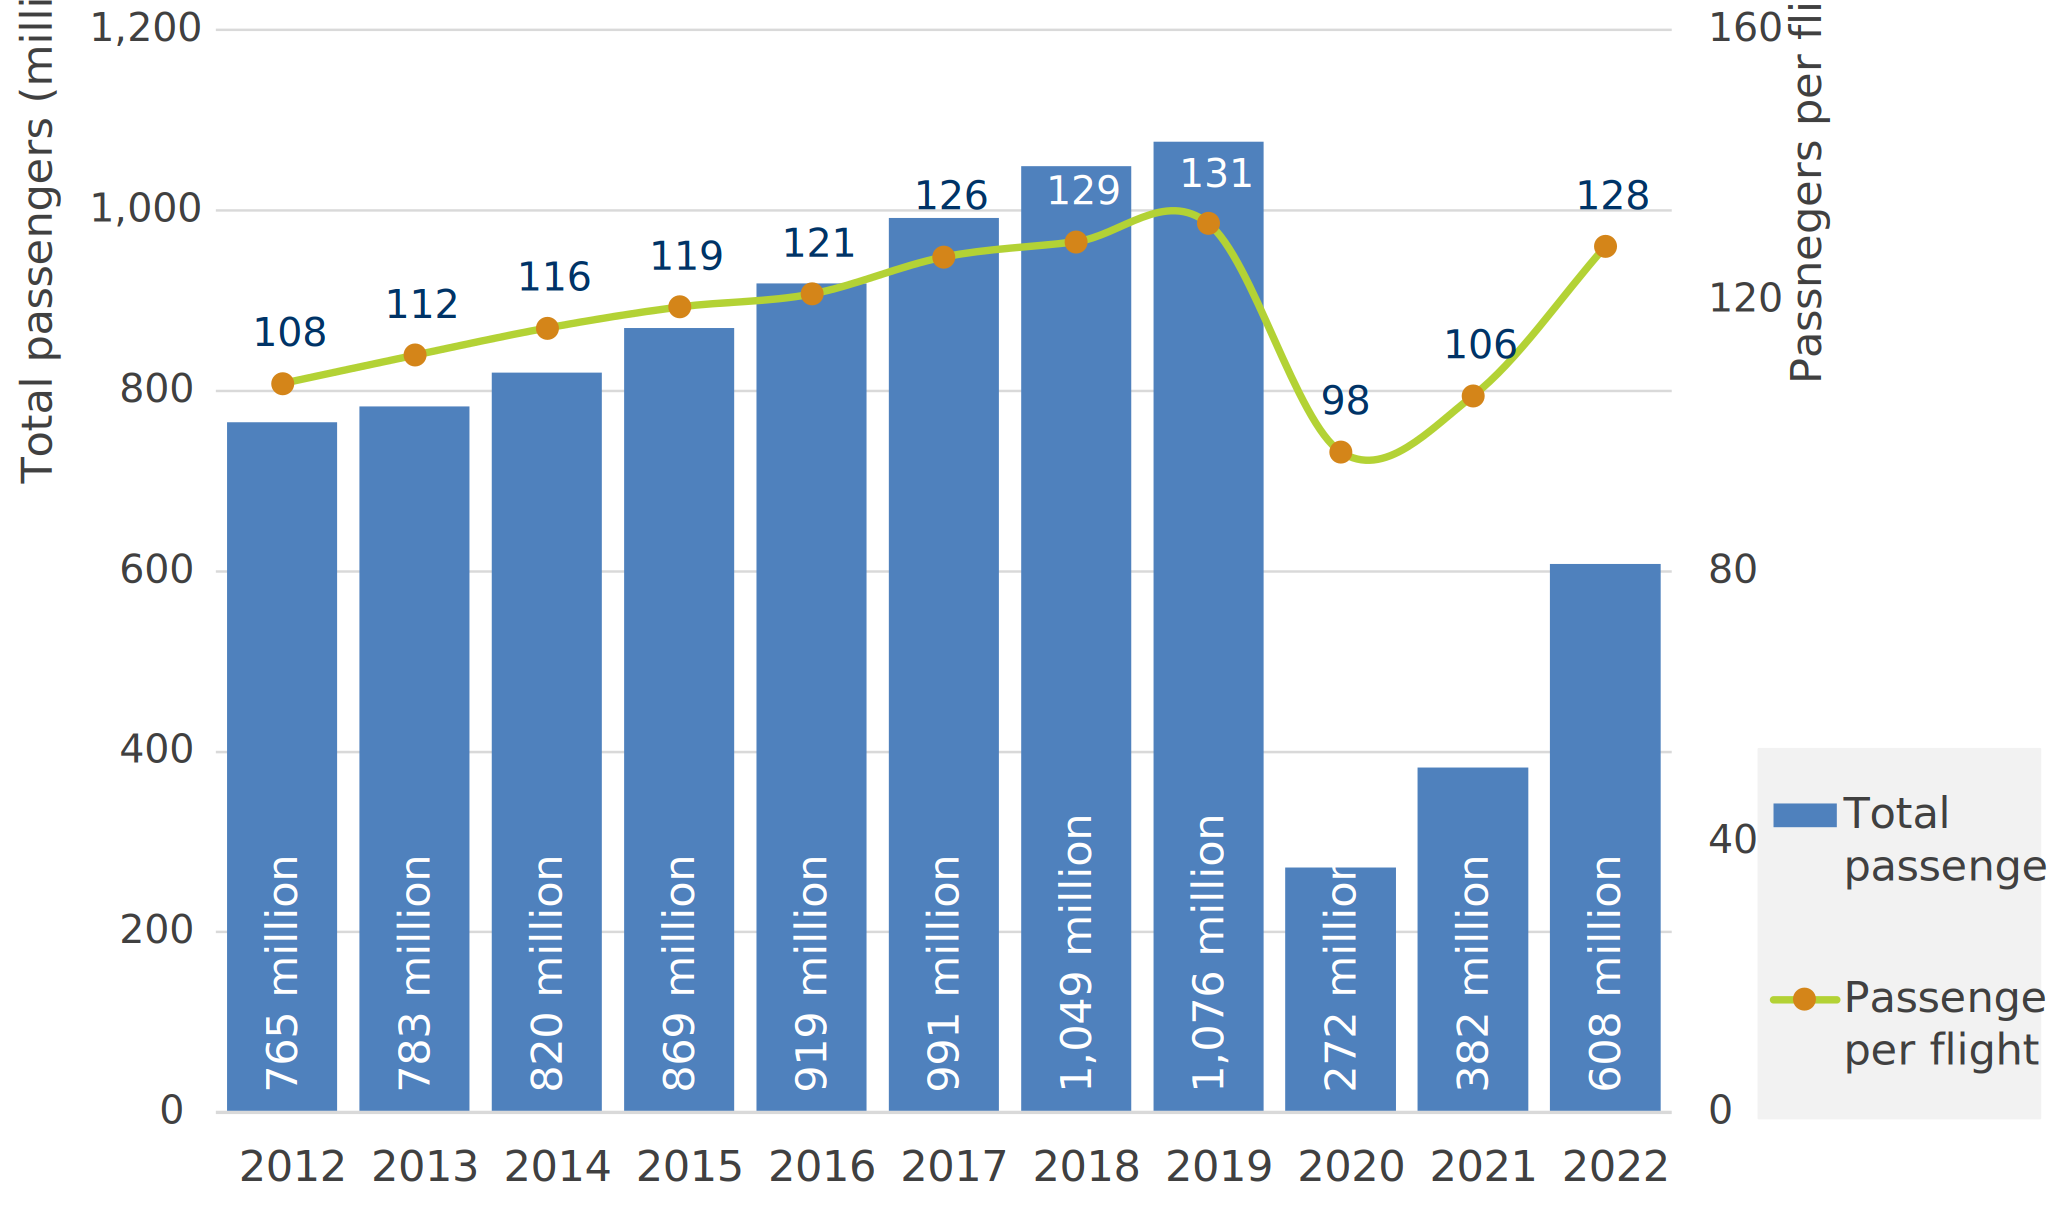
\includegraphics{chapters/../figures/number_passengers.png}

}

\caption{\label{fig-number-of-passengers}Number of passengers per flight
in ECAC 2012-2021 \protect\hyperlink{ref-ectrl:statfor:sid}{{[}5{]}}}

\end{figure}

\hypertarget{when-to-use-the-input-6}{%
\section{When to use the input?}\label{when-to-use-the-input-6}}

This input is suitable to be used in any analysis that requires
historical data on the number of passengers per flight and/or per
movement.

\hypertarget{comments-5}{%
\section{Comments}\label{comments-5}}

The Eurostat air transport domain contains national and international
intra- and extra-EU data. This provides air transport data for
passengers (in numbers of passengers) and for freight and mail (in
thousands of tonnes), as well as air traffic data for airports, airlines
and aircraft. Data are transmitted to Eurostat by the Member States of
the European Union as well as the candidate countries Iceland, Norway
and Switzerland. The air transport data have been calculated using data
collected at airports.

The average number of passengers per movement\footnote{A movement is
  either a take-off or a landing at an airport} for a given year is
obtained by dividing the number of `departing passengers on board' by
the number of `departing flights for that year'.

\hypertarget{related-inputs-10}{%
\section{Related inputs}\label{related-inputs-10}}

Chapter~\ref{sec-number-of-ifr-flights}
\protect\hyperlink{sec-number-of-ifr-flights}{Number of IFR flights}

\hypertarget{references-13}{%
\section{References}\label{references-13}}

\hypertarget{sec-cancellation-cost}{%
\chapter{Cancellation cost}\label{sec-cancellation-cost}}

\hypertarget{eurocontrol-recommended-values-11}{%
\section{EUROCONTROL recommended
values}\label{eurocontrol-recommended-values-11}}

In Table~\ref{tbl-cancel-cost} is presented the average cost of
cancellation of a commercial flight on the day of operation, adjusted
from 2014 to 2022 prices. The values are provided for different types of
aircraft, based on the number of seats.

\hypertarget{tbl-cancel-cost}{}
\setlength{\LTpost}{0mm}
\begin{longtable}{lrrrrrr}
\caption{\label{tbl-cancel-cost}Average cost of cancellation of a commercial flight on the day of
operation }\tabularnewline

\toprule
 & \multicolumn{4}{c}{Narrow-body} & \multicolumn{2}{c}{Wide-body} \\ 
\cmidrule(lr){2-5} \cmidrule(lr){6-7}
 & \multicolumn{3}{c}{Traditional network carrier} & Low-cost carrier & \multicolumn{2}{c}{Traditional network carrier } \\ 
\cmidrule(lr){2-4} \cmidrule(lr){5-5} \cmidrule(lr){6-7}
Seats & 50 & 120 & 180 & 189 & 250 & 400 \\ 
\midrule
Cost of cancellation & $\text{EUR}6,790$ & $\text{EUR}16,640$ & $\text{EUR}25,720$ & $\text{EUR}18,570$ & $\text{EUR}85,570$ & $\text{EUR}123,900$ \\ 
of which passenger care and compensation & $\text{EUR}3,100$ & $\text{EUR}7,600$ & $\text{EUR}12,400$ & $\text{EUR}17,500$ & $\text{EUR}40,500$ & $\text{EUR}64,800$ \\ 
\bottomrule
\end{longtable}
\begin{minipage}{\linewidth}
\emph{Source: Data supplied by the airline members of the SESAR CBA team and expert judgment derived from an analysis of 2012 total flights carried out in Europe}\\
\end{minipage}

\begin{tcolorbox}[enhanced jigsaw, opacityback=0, arc=.35mm, colframe=quarto-callout-note-color-frame, breakable, left=2mm, leftrule=.75mm, titlerule=0mm, colbacktitle=quarto-callout-note-color!10!white, rightrule=.15mm, opacitybacktitle=0.6, bottomtitle=1mm, colback=white, toptitle=1mm, title=\textcolor{quarto-callout-note-color}{\faInfo}\hspace{0.5em}{Note}, bottomrule=.15mm, toprule=.15mm, coltitle=black]

Traditional carrier estimates can be used for regional carriers

\end{tcolorbox}

An \textbf{alternative value} encompassing the \textbf{system-wide
average cancellation cost} was also estimated by the experts, amounting
approximately \textbf{€20,930} (adjusted from 2014 to 2022 prices).

\hypertarget{description-4}{%
\section{Description}\label{description-4}}

The values presented above refer to cancellation on the day of operation
and include the following:

\begin{itemize}
\item
  Service recovery costs (i.e.~passenger care and compensation costs
  (passenger vouchers, drinks, telephone calls, hotels))
\item
  Loss of revenue
\item
  Interlining costs
\item
  Loss of future value (i.e.~passenger opportunity cost (individual
  passenger delay expressed in value))
\item
  Crew and catering costs
\item
  Passenger compensation for denied boarding and missed connections,
  estimated based on the application of the Regulation (EC) No
  261/2004.\protect\hyperlink{ref-eureg2612004}{{[}37{]}}
\item
  Luggage delivery costs
\item
  Operational savings (e.g.~fuel, airport and navigation fees,
  maintenance, handling outstations, lounge outstations)
\end{itemize}

Ground handling costs (e.g.~ramp services, passenger services and field
operation services) are not included in the estimation.

\hypertarget{comments-6}{%
\section{Comments}\label{comments-6}}

When a flight is carried out, the airline incurs out-of-pocket expenses
(i.e.~variable costs) but receives revenues which are 60 100\% greater
than the out-of-pocket expenses. Cancelling a flight means that the
airline forgoes a substantial operating profit. Also, in addition to the
loss, costs are incurred for the care and compensation of passengers.

\begin{figure}

{\centering 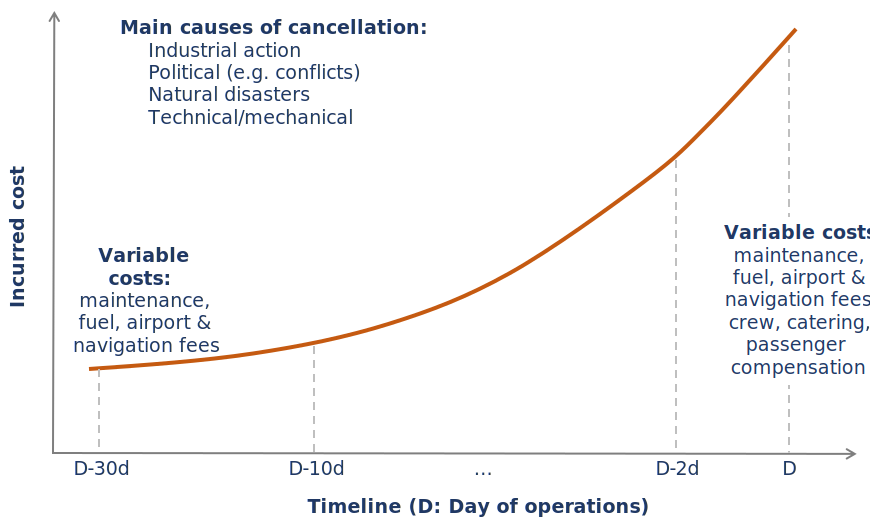
\includegraphics{chapters/../figures/cancellation_function.svg}

}

\caption{\label{fig-cancel-function}Cancellation costs as a function of
time}

\end{figure}

Timely cancellation will enable the airline to take the necessary
measures to mitigate the cost impact, for example by rebooking
passengers on another flight and allocating crew and aircraft to a
different destination. The cancellation costs will thus be minimal and
more in the region of the incurred opportunity cost and passenger value
of time. If the cancellation is nearer the flight time (i.e.~on the day
of operation (D)), the cost of cancellation increases, to cover expenses
such as fuel, maintenance, and crew and catering.

\hypertarget{related-inputs-11}{%
\section{Related inputs}\label{related-inputs-11}}

Chapter~\ref{sec-operational-cancellation-rate}
\protect\hyperlink{sec-operational-cancellation-rate}{Operational
cancellation rate}

\hypertarget{references-14}{%
\section{References}\label{references-14}}

\hypertarget{sec-operational-cancellation-rate}{%
\chapter{Operational cancellation
rate}\label{sec-operational-cancellation-rate}}

\hypertarget{eurocontrol-recommended-values-12}{%
\section{EUROCONTROL recommended
values}\label{eurocontrol-recommended-values-12}}

Below is presented the rate of IFR flight cancellations in Europe.

\begin{figure}

{\centering 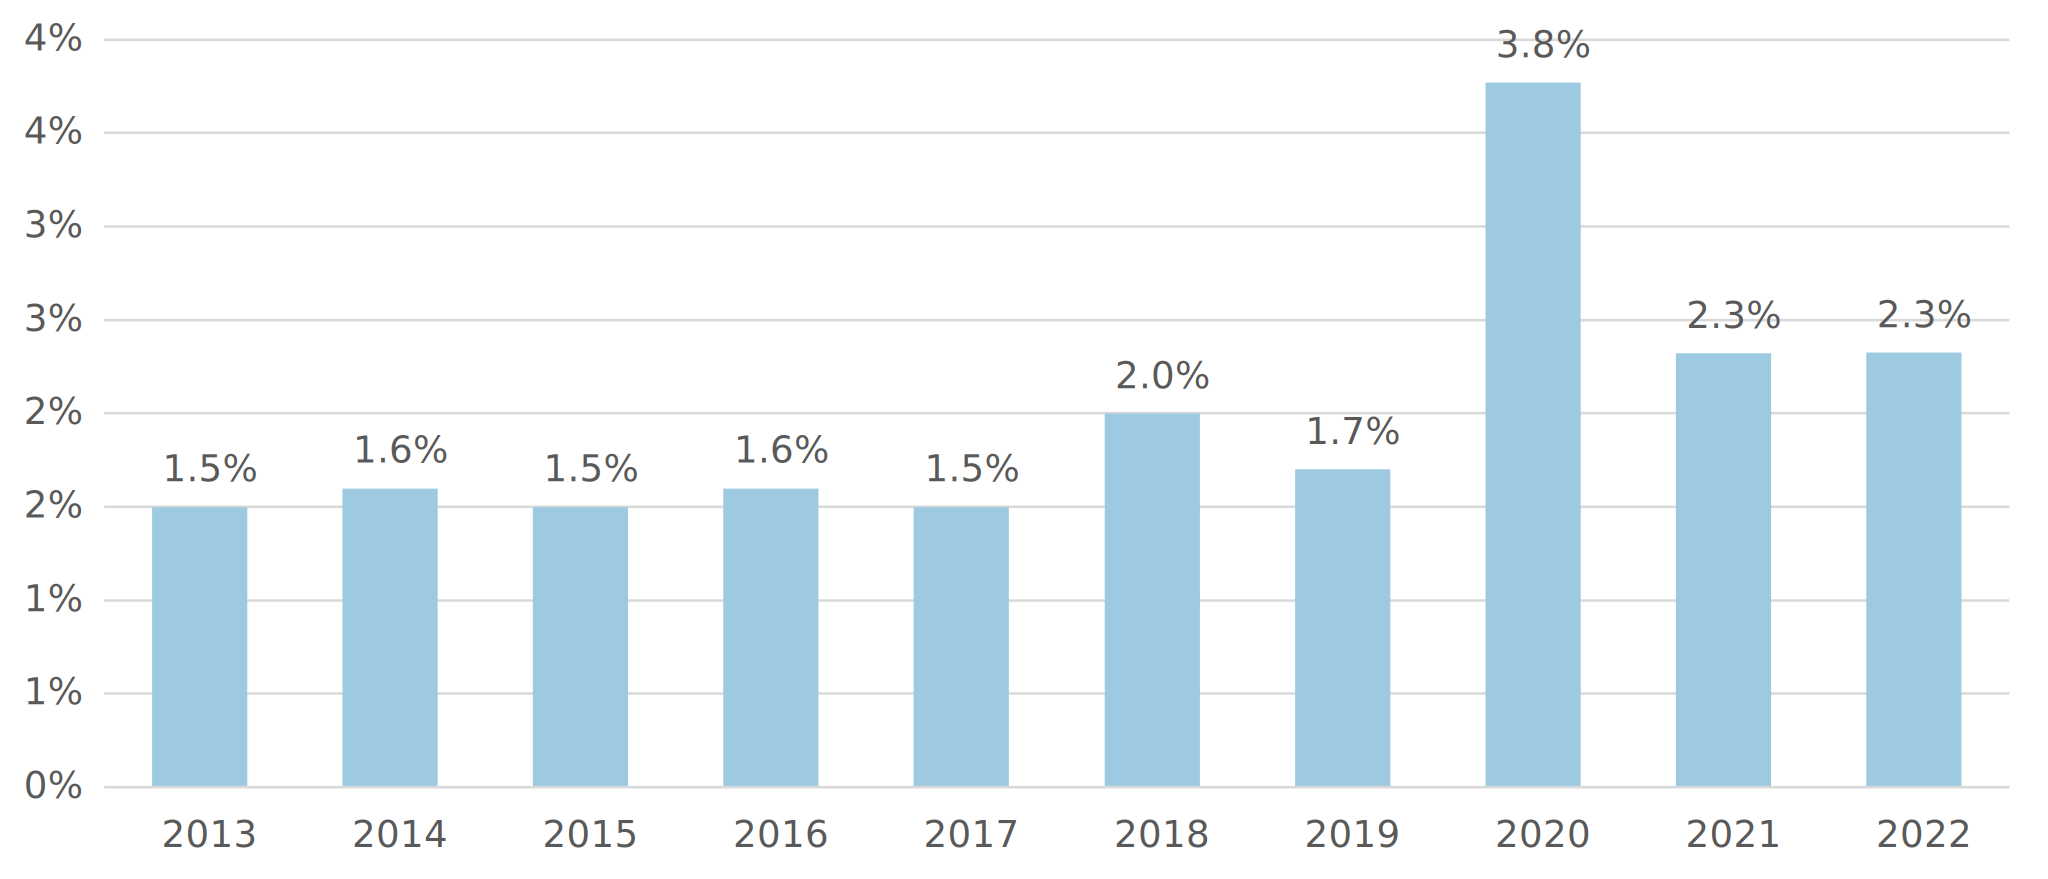
\includegraphics{chapters/../figures/cancellation_rate.svg}

}

\caption{\label{fig-cancellation-rate}Operational cancellation rate in
Europe}

\end{figure}

\emph{Source: EUROCONTROL data. Detailed data are available upon
request}

Reports about all causes of delay (and cancellation up 2019) are
available in the \href{https://www.eurocontrol.int/library}{EUROCONTROL
library}.

\begin{tcolorbox}[enhanced jigsaw, opacityback=0, arc=.35mm, colframe=quarto-callout-note-color-frame, breakable, left=2mm, leftrule=.75mm, titlerule=0mm, colbacktitle=quarto-callout-note-color!10!white, rightrule=.15mm, opacitybacktitle=0.6, bottomtitle=1mm, colback=white, toptitle=1mm, title=\textcolor{quarto-callout-note-color}{\faInfo}\hspace{0.5em}{Note}, bottomrule=.15mm, toprule=.15mm, coltitle=black]

In 2020 the COVID-19 pandemic strongly influenced the entire aviation
industry with more than double cancellation rate then in 2019.

\end{tcolorbox}

\hypertarget{description-5}{%
\section{Description}\label{description-5}}

According to Annex IV of Commission Implementing Regulation EU No
390/2013, \protect\hyperlink{ref-eureg:3902013}{{[}38{]}} an
`operational cancellation' means an arrival or departure of a scheduled
flight to which the following conditions apply:

\begin{itemize}
\item
  the flight received an airport slot; and
\item
  the flight was confirmed by the air carrier the day before operations
  and/or it featured in the daily list of flight schedules produced by
  the airport operator the day before of operations; but
\item
  the actual landing or take-off did not occur.
\end{itemize}

\hypertarget{references-15}{%
\section{References}\label{references-15}}

\hypertarget{sec-cost-of-delay}{%
\chapter{Cost of delay}\label{sec-cost-of-delay}}

\hypertarget{eurocontrol-recommended-values-13}{%
\section{EUROCONTROL recommended
values}\label{eurocontrol-recommended-values-13}}

The tables below present an overview of the \textbf{average cost per
minute to the airline of ground or airborne delay of a commercial
passenger flight}. Please note that all the numbers are based on studies
performed by the University of Westminster
\protect\hyperlink{ref-uow:2004}{{[}39{]}}
\protect\hyperlink{ref-uow:2015}{{[}40{]}} and are adjusted to 2022
prices based on \protect\hyperlink{tbl-inflation-table}{inflation}.

The figures presented in this section constitute high-level averages and
are valid as indicative estimates. \textbf{It is strongly recommended
that they are used as indicators or for general insights into delay
costs and not for specific analyses or operational planning.} Different
values may be obtained for other contexts (e.g.~other airspace areas or
airports (hub or non-hub), etc.), with different aircraft and delay
distributions.

\hypertarget{tbl-delay-cost-tact}{}
\setlength{\LTpost}{0mm}
\begin{longtable}{lrr}
\caption{\label{tbl-delay-cost-tact}Tactical delay cost with network effect per minute }\tabularnewline

\toprule
Flight phase & All delays (0 to >300 min) & Short delays (<30 min) \\ 
\midrule
\multicolumn{3}{l}{Ground} \\ 
\midrule
At gate & $\text{EUR}165.91$ & $\text{EUR}45.03$ \\ 
Taxiing in/out & $\text{EUR}182.50$ & $\text{EUR}61.62$ \\ 
\midrule
\multicolumn{3}{l}{Airborne} \\ 
\midrule
En-route (cruise extension) & $\text{EUR}212.12$ & $\text{EUR}88.88$ \\ 
Arrival management & $\text{EUR}206.20$ & $\text{EUR}84.14$ \\ 
\bottomrule
\end{longtable}
\begin{minipage}{\linewidth}
\emph{Source: calculated based on \href{https://www.eurocontrol.int/publication/european-airline-delay-cost-reference-values}{University of Westminster (2015), European airline delay cost reference values - version 4.1}. Also available in \href{https://www.eurocontrol.int/publication/evaluating-true-cost-airlines-one-minute-airborne-or-ground-delay}{2004 iteration}}\\
\end{minipage}

\hypertarget{tbl-delay-cost-strat}{}
\setlength{\LTpost}{0mm}
\begin{longtable}{lr}
\caption{\label{tbl-delay-cost-strat}Strategic delay cost }\tabularnewline

\toprule
\textbf{Flight phase} & \textbf{Cost per minute} \\ 
\midrule
\multicolumn{2}{l}{Ground} \\ 
\midrule
At-Gate & $\text{EUR}17.78$ \\ 
Taxi in / out & $\text{EUR}46.69$ \\ 
\midrule
\multicolumn{2}{l}{Airborne} \\ 
En-Route (cruise extension) & $\text{EUR}82.95$ \\ 
\bottomrule
\end{longtable}
\begin{minipage}{\linewidth}
\emph{Source: calculated based on \href{https://www.eurocontrol.int/publication/european-airline-delay-cost-reference-values}{University of Westminster (2015), European airline delay cost reference values - version 4.1}. Also available in \href{https://www.eurocontrol.int/publication/evaluating-true-cost-airlines-one-minute-airborne-or-ground-delay}{2004} and 2011 iterations}\\
\end{minipage}

On top of the above, the \textbf{network average cost of ATFM
delay\footnote{ATFM delay is defined as the duration between the last
  take-off time requested by the aircraft operator and the take-off slot
  allocated by the Network Manager following a regulation communicated
  by the flow management position (FMP), in relation to an airport
  (airport ATFM delay) or sector location (en route ATFM delay)} amounts
€100 per minute.}

The University of Westminster (UoW) report, published in 2004 and
updated in 2011 and 2015, represents the most recent and comprehensive
appraisal of the cost of delay in the air traffic management system in
Europe. The report is designed as a reference document for European
delay direct costs incurred by airlines, both at strategic (planning)
and tactical stages.

It contains a detailed assessment of the delay cost for 15 specific
aircraft types (extended from 12 in the previous report versions),
taking into account crew, fuel, fleet, maintenance and passenger
additional costs due to delay. Note that the list of aircraft used for
this report does not include some recent types such as Airbus NEO
Series, A220, A350 or B787.

In the study, costs are assigned under three cost scenarios: low, base
and high. These scenarios are designed to cover the probable range of
costs for European operators. The base cost scenario is, to the greatest
extent possible, designed to reflect the typical case and is, therefore,
the one used in this value.

The University of Westminster report presents costs of delay in four
flight phases: at gate, taxiing, en-route (cruise extension) and arrival
management. For accuracy reasons, the definitions used by the University
of Westminster are presented as such. They are extracted from the UoW
2004 and 2011 reports.

\hypertarget{flight-phases-types-of-delay-costs-and-calculation-method-used}{%
\section{Flight phases, types of delay costs and calculation method
used}\label{flight-phases-types-of-delay-costs-and-calculation-method-used}}

A description of the flight phases, types of delay costs and the
calculation method used in the study are given hereafter.

\begin{figure}

{\centering 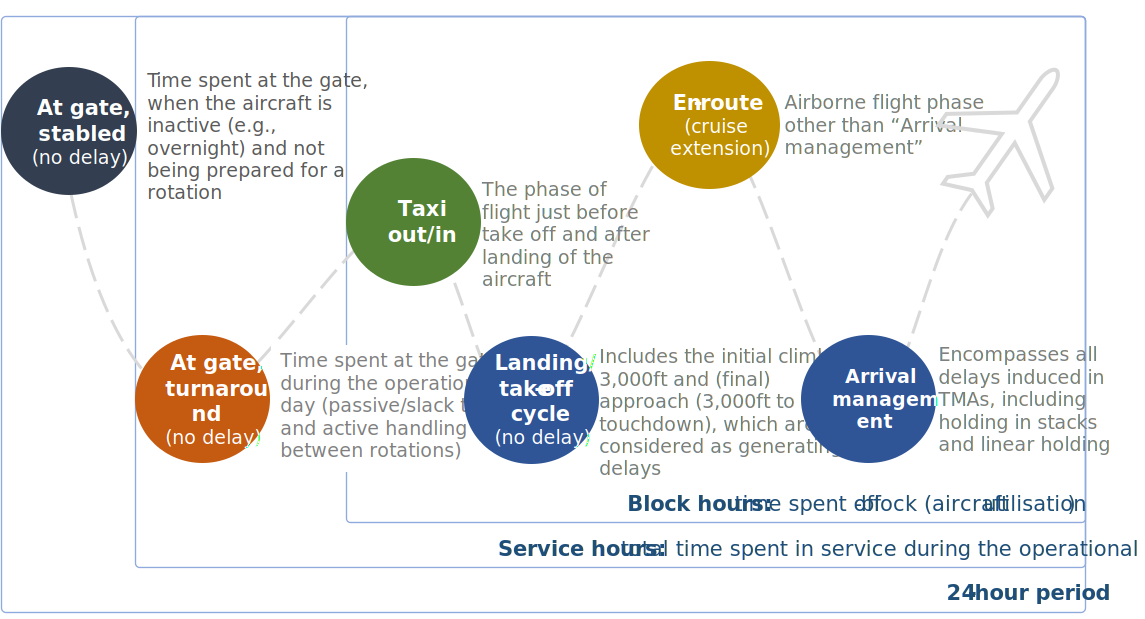
\includegraphics{chapters/../figures/flight_phases.svg}

}

\caption{\label{fig-flight-phases}Overview of the different flight
phases}

\end{figure}

\textbf{\emph{Types of delay costs}}

\begin{itemize}
\item
  Tactical delay costs are incurred on the day of operations. In most
  cases, it is anticipated that the user will find it appropriate to use
  the full tactical costs in order to calculate these costs of delay.
  These include the reactionary costs of `knock-on' delay in the rest of
  the network, which it is usually pertinent to include.
\item
  Strategic delay costs are accounted for in advance. Strategic costs
  are typically used to assess the cost of adding buffers to schedules.
  This could be by airline choice or imposed by scheduling constraints
  at an airport (and thus considered a cost of congestion, albeit one
  which offsets tactical delay costs). Strategic costs may also be
  incurred as a consequence of factors which contribute to an increase
  in flight time in a predictable way, such as delay due to route
  design.
\end{itemize}

\textbf{\emph{Calculation method}}

The tactical and strategic delay costs referred to in
Table~\ref{tbl-delay-cost-tact} and Table~\ref{tbl-delay-cost-strat} are
calculated based on the results extracted from the University of
Westminster (UoW) study report ``European airline delay cost reference
values -- Updated and extended values Version 4.1'' -- December 2015.
Explicit cost tables for analytical use (up to 30 minutes of delay) are
presented at the end of this section. The extended tables can be found
in the UoW report mentioned above.

As regards tactical delay costs, these are given for 5, 15, 30, 60, 90,
120, 180, 240 and 300 minutes in the UoW report. These are scaled up to
network level, because on the day of operations, original delays caused
by one aircraft cause `knock-on' effects in the rest of the network
(reactionary delays).

Based on at-gate data provided by the Central Office for Delay Analysis
(CODA) on ranges of departure delays by aircraft type for year 2014,
assumptions have been made for the remaining three flight phases
(i.e.~taxi, en-route and arrival management). The same delay
distribution has been used as an assumption applicable to all flight
phases.

The UoW results have been averaged by minute of delay per type of
aircraft (15 in total) and further weighted by the distribution of the
number of delayed flights per delay range, at departure, carried out by
these aircraft in 2014.

Consequently, for each flight phase, two types of values have been
calculated:

\begin{enumerate}
\def\labelenumi{\arabic{enumi}.}
\item
  one taking into account long delays (i.e.~0 to more than 300 minutes)
\item
  one taking into account short delays (i.e.~up to 30 minutes), which
  represent about 90\% of all delays
\end{enumerate}

As regards strategic delay, since costs at the strategic level are
incorporated into the aircraft operator's schedule in advance, they are
associated with average costs and, therefore, only a distribution of the
number of flights was applied in order to calculate the strategic
high-level averages.

\begin{tcolorbox}[enhanced jigsaw, opacityback=0, arc=.35mm, colframe=quarto-callout-tip-color-frame, breakable, left=2mm, leftrule=.75mm, titlerule=0mm, colbacktitle=quarto-callout-tip-color!10!white, rightrule=.15mm, opacitybacktitle=0.6, bottomtitle=1mm, colback=white, toptitle=1mm, title=\textcolor{quarto-callout-tip-color}{\faLightbulb}\hspace{0.5em}{Use of costs in business cases}, bottomrule=.15mm, toprule=.15mm, coltitle=black]

When comparing two scenarios, it is not correct to calculate the delay
avoided as a benefit without taking into account the corresponding
marginal cost of capacity. In other words, there is a delay threshold
below which the marginal cost of capacity outweighs the delay avoidance
benefit.

Every CBA should carefully consider whether the improvements envisaged
by the project are of a tactical or strategic nature. For the correct
use and precise understanding of the tactical and strategic delay
concepts, see section 4 of and Annex I to the 2004 University of
Westminster delay study.

\end{tcolorbox}

\hypertarget{delay-cost-details-by-aircraft-type-and-duration}{%
\subsection{Delay cost details by aircraft type and
duration}\label{delay-cost-details-by-aircraft-type-and-duration}}

In the tables below are presented the explicit cost data as extracted
from University of Westminster study and adjusted to 2022 prices.

\hypertarget{tbl-delay-cost-total-tact}{}
\setlength{\LTpost}{0mm}
\begin{longtable}{lrrrrrrrrrrrr}
\caption{\label{tbl-delay-cost-total-tact}Total tactical delay costs with network effect - base scenario }\tabularnewline

\toprule
 & \multicolumn{3}{c}{At gate} & \multicolumn{3}{c}{Taxiing} & \multicolumn{3}{c}{En-route} & \multicolumn{3}{c}{Arrival management} \\ 
\cmidrule(lr){2-4} \cmidrule(lr){5-7} \cmidrule(lr){8-10} \cmidrule(lr){11-13}
Aircraft type & 5' & 15' & 30' & 5' & 15' & 30' & 5' & 15' & 30' & 5' & 15' & 30' \\ 
\midrule
A319 & $\text{EUR}83$ & $\text{EUR}523$ & $\text{EUR}1,901$ & $\text{EUR}154$ & $\text{EUR}724$ & $\text{EUR}2,305$ & $\text{EUR}286$ & $\text{EUR}1,128$ & $\text{EUR}3,112$ & $\text{EUR}262$ & $\text{EUR}1,057$ & $\text{EUR}2,982$ \\ 
A320 & $\text{EUR}95$ & $\text{EUR}594$ & $\text{EUR}2,162$ & $\text{EUR}178$ & $\text{EUR}844$ & $\text{EUR}2,672$ & $\text{EUR}297$ & $\text{EUR}1,199$ & $\text{EUR}3,386$ & $\text{EUR}297$ & $\text{EUR}1,187$ & $\text{EUR}3,350$ \\ 
A321 & $\text{EUR}119$ & $\text{EUR}689$ & $\text{EUR}2,566$ & $\text{EUR}201$ & $\text{EUR}927$ & $\text{EUR}3,041$ & $\text{EUR}357$ & $\text{EUR}1,414$ & $\text{EUR}4,015$ & $\text{EUR}333$ & $\text{EUR}1,343$ & $\text{EUR}3,873$ \\ 
A332 & $\text{EUR}213$ & $\text{EUR}1,176$ & $\text{EUR}4,218$ & $\text{EUR}404$ & $\text{EUR}1,722$ & $\text{EUR}5,310$ & $\text{EUR}677$ & $\text{EUR}2,542$ & $\text{EUR}6,961$ & $\text{EUR}558$ & $\text{EUR}2,185$ & $\text{EUR}6,237$ \\ 
AT43 & $\text{EUR}36$ & $\text{EUR}213$ & $\text{EUR}724$ & $\text{EUR}71$ & $\text{EUR}309$ & $\text{EUR}915$ & $\text{EUR}83$ & $\text{EUR}345$ & $\text{EUR}986$ & $\text{EUR}83$ & $\text{EUR}345$ & $\text{EUR}986$ \\ 
AT72 & $\text{EUR}47$ & $\text{EUR}286$ & $\text{EUR}974$ & $\text{EUR}83$ & $\text{EUR}392$ & $\text{EUR}1,199$ & $\text{EUR}107$ & $\text{EUR}463$ & $\text{EUR}1,343$ & $\text{EUR}107$ & $\text{EUR}440$ & $\text{EUR}1,295$ \\ 
B733 & $\text{EUR}83$ & $\text{EUR}511$ & $\text{EUR}1,842$ & $\text{EUR}166$ & $\text{EUR}749$ & $\text{EUR}2,317$ & $\text{EUR}297$ & $\text{EUR}1,140$ & $\text{EUR}3,112$ & $\text{EUR}250$ & $\text{EUR}1,010$ & $\text{EUR}2,851$ \\ 
B734 & $\text{EUR}95$ & $\text{EUR}570$ & $\text{EUR}2,067$ & $\text{EUR}178$ & $\text{EUR}820$ & $\text{EUR}2,577$ & $\text{EUR}309$ & $\text{EUR}1,199$ & $\text{EUR}3,326$ & $\text{EUR}297$ & $\text{EUR}1,164$ & $\text{EUR}3,243$ \\ 
B735 & $\text{EUR}83$ & $\text{EUR}463$ & $\text{EUR}1,663$ & $\text{EUR}166$ & $\text{EUR}712$ & $\text{EUR}2,150$ & $\text{EUR}274$ & $\text{EUR}1,045$ & $\text{EUR}2,816$ & $\text{EUR}213$ & $\text{EUR}879$ & $\text{EUR}2,483$ \\ 
B738 & $\text{EUR}107$ & $\text{EUR}641$ & $\text{EUR}2,305$ & $\text{EUR}178$ & $\text{EUR}856$ & $\text{EUR}2,745$ & $\text{EUR}321$ & $\text{EUR}1,283$ & $\text{EUR}3,599$ & $\text{EUR}297$ & $\text{EUR}1,211$ & $\text{EUR}3,457$ \\ 
B744 & $\text{EUR}286$ & $\text{EUR}1,627$ & $\text{EUR}5,939$ & $\text{EUR}546$ & $\text{EUR}2,400$ & $\text{EUR}7,484$ & $\text{EUR}1,104$ & $\text{EUR}4,086$ & $\text{EUR}10,857$ & $\text{EUR}844$ & $\text{EUR}3,279$ & $\text{EUR}9,242$ \\ 
B752 & $\text{EUR}119$ & $\text{EUR}736$ & $\text{EUR}2,720$ & $\text{EUR}237$ & $\text{EUR}1,093$ & $\text{EUR}3,445$ & $\text{EUR}404$ & $\text{EUR}1,592$ & $\text{EUR}4,431$ & $\text{EUR}345$ & $\text{EUR}1,402$ & $\text{EUR}4,062$ \\ 
B763 & $\text{EUR}201$ & $\text{EUR}1,069$ & $\text{EUR}3,802$ & $\text{EUR}345$ & $\text{EUR}1,497$ & $\text{EUR}4,656$ & $\text{EUR}606$ & $\text{EUR}2,281$ & $\text{EUR}6,225$ & $\text{EUR}570$ & $\text{EUR}2,173$ & $\text{EUR}6,022$ \\ 
DH8D & $\text{EUR}47$ & $\text{EUR}297$ & $\text{EUR}1,057$ & $\text{EUR}83$ & $\text{EUR}404$ & $\text{EUR}1,272$ & $\text{EUR}130$ & $\text{EUR}534$ & $\text{EUR}1,520$ & $\text{EUR}130$ & $\text{EUR}534$ & $\text{EUR}1,520$ \\ 
E190 & $\text{EUR}71$ & $\text{EUR}380$ & $\text{EUR}1,366$ & $\text{EUR}130$ & $\text{EUR}558$ & $\text{EUR}1,722$ & $\text{EUR}213$ & $\text{EUR}832$ & $\text{EUR}2,269$ & $\text{EUR}213$ & $\text{EUR}820$ & $\text{EUR}2,234$ \\ 
\bottomrule
\end{longtable}
\begin{minipage}{\linewidth}
\emph{Source: \href{https://www.eurocontrol.int/publication/european-airline-delay-cost-reference-values}{University of Westminster (2015), European airline delay cost reference values - version 4.1}}\\
\end{minipage}

\hypertarget{tbl-delay-cost-hour}{}
\setlength{\LTpost}{0mm}
\begin{longtable}{lrrr}
\caption{\label{tbl-delay-cost-hour}Strategic delay costs per hour - base scenario }\tabularnewline

\toprule
Aircraft type & At gate & Taxiing & En-route \\ 
\midrule
A319 & $\text{EUR}962.25$ & $\text{EUR}2,281.20$ & $\text{EUR}4,062.31$ \\ 
B734 & $\text{EUR}1,068.90$ & $\text{EUR}2,565.61$ & $\text{EUR}4,145.26$ \\ 
B735 & $\text{EUR}1,247.84$ & $\text{EUR}2,756.40$ & $\text{EUR}4,906.05$ \\ 
B738 & $\text{EUR}2,043.00$ & $\text{EUR}5,036.41$ & $\text{EUR}8,576.12$ \\ 
B752 & $\text{EUR}273.74$ & $\text{EUR}891.15$ & $\text{EUR}1,068.90$ \\ 
B763 & $\text{EUR}404.10$ & $\text{EUR}1,163.71$ & $\text{EUR}1,508.55$ \\ 
B744 & $\text{EUR}641.11$ & $\text{EUR}2,031.15$ & $\text{EUR}3,801.60$ \\ 
A319 & $\text{EUR}712.21$ & $\text{EUR}2,220.76$ & $\text{EUR}3,908.25$ \\ 
A320 & $\text{EUR}605.55$ & $\text{EUR}2,031.15$ & $\text{EUR}3,504.16$ \\ 
A321 & $\text{EUR}1,199.26$ & $\text{EUR}2,458.95$ & $\text{EUR}4,336.05$ \\ 
AT43 & $\text{EUR}1,782.30$ & $\text{EUR}5,892.01$ & $\text{EUR}13,006.97$ \\ 
AT72 & $\text{EUR}855.60$ & $\text{EUR}2,839.35$ & $\text{EUR}5,000.86$ \\ 
DH8D & $\text{EUR}1,555.95$ & $\text{EUR}4,014.91$ & $\text{EUR}7,400.56$ \\ 
E190 & $\text{EUR}641.11$ & $\text{EUR}1,354.50$ & $\text{EUR}1,936.35$ \\ 
A332 & $\text{EUR}914.85$ & $\text{EUR}2,043.00$ & $\text{EUR}3,267.15$ \\ 
\bottomrule
\end{longtable}
\begin{minipage}{\linewidth}
\emph{Source: \href{https://www.eurocontrol.int/publication/european-airline-delay-cost-reference-values}{University of Westminster (2015), European airline delay cost reference values - version 4.1}}\\
\end{minipage}

\hypertarget{related-inputs-12}{%
\section{Related inputs}\label{related-inputs-12}}

Chapter~\ref{sec-air-traffic-statistics-and-forecasts}
\protect\hyperlink{sec-air-traffic-statistics-and-forecasts}{Air traffic
statistics and forecasts}

Chapter~\ref{sec-air-traffic-delay}
\protect\hyperlink{sec-air-traffic-delay}{Air traffic delay}

\hypertarget{references-16}{%
\section{References}\label{references-16}}

\hypertarget{sec-cost-of-diversions}{%
\chapter{Cost of diversion}\label{sec-cost-of-diversions}}

\hypertarget{eurocontrol-recommended-values-14}{%
\section{EUROCONTROL recommended
values}\label{eurocontrol-recommended-values-14}}

Table~\ref{tbl-diversion-comm} and Table~\ref{tbl-diversion-bus} present
the estimated cost of diversion of a flight to an airport other than the
one initially planned. The values are split between commercial and
business aviation, and, where available, represent a range of values as
estimated by the airline members consulted.

\hypertarget{tbl-diversion-comm}{}
\setlength{\LTpost}{0mm}
\begin{longtable}{lr}
\caption{\label{tbl-diversion-comm}Estimated cost of diversion for commercial aviation }\tabularnewline

\toprule
Type of flight & Cost of diverted flight\textsuperscript{1} \\ 
\midrule
Regional flights & $\text{EUR}1,000$–$\text{EUR}7,000$ \\ 
Continental flights & $\text{EUR}1,400$–$\text{EUR}10,500$ \\ 
Intercontinental flights & $\text{EUR}7,000$–$\text{EUR}77,200$ \\ 
\bottomrule
\end{longtable}
\begin{minipage}{\linewidth}
\textsuperscript{1}Monetary values were adjusted from 2006 to 2022 prices according to inflation\\
\emph{Source: Data supplied by the airline members of the SESAR evaluation team, derived from an analysis of 2006 ECAC data}\\
\end{minipage}

\begin{tcolorbox}[enhanced jigsaw, opacityback=0, arc=.35mm, colframe=quarto-callout-note-color-frame, breakable, left=2mm, leftrule=.75mm, titlerule=0mm, colbacktitle=quarto-callout-note-color!10!white, rightrule=.15mm, opacitybacktitle=0.6, bottomtitle=1mm, colback=white, toptitle=1mm, title=\textcolor{quarto-callout-note-color}{\faInfo}\hspace{0.5em}{Note}, bottomrule=.15mm, toprule=.15mm, coltitle=black]

The penalties associated with the late delivery of cargo are not
considered in the estimation, as this type of data is not yet readily
available.

\end{tcolorbox}

\hypertarget{tbl-diversion-bus}{}
\setlength{\LTpost}{0mm}
\begin{longtable}{lr}
\caption{\label{tbl-diversion-bus}Estimated cost of diversion for business aviation }\tabularnewline

\toprule
Type of flight & Cost of diverted flight\textsuperscript{1} \\ 
\midrule
Business aviation & $\text{EUR}8,800$ \\ 
\bottomrule
\end{longtable}
\begin{minipage}{\linewidth}
\textsuperscript{1}Monetary values were adjusted from 2012 to 2022 prices according to inflation\\
\emph{Source: Data supplied by the airline members of the SESAR CBA team (2015)}\\
\end{minipage}

\begin{tcolorbox}[enhanced jigsaw, opacityback=0, arc=.35mm, colframe=quarto-callout-note-color-frame, breakable, left=2mm, leftrule=.75mm, titlerule=0mm, colbacktitle=quarto-callout-note-color!10!white, rightrule=.15mm, opacitybacktitle=0.6, bottomtitle=1mm, colback=white, toptitle=1mm, title=\textcolor{quarto-callout-note-color}{\faInfo}\hspace{0.5em}{Note}, bottomrule=.15mm, toprule=.15mm, coltitle=black]

The estimated cost for business aviation assumes that for each diverted
flight there is one additional positioning flight.

\end{tcolorbox}

In 2022, out of the total number of flights (9.3 million) with a
destination in EUROCONTROL Network Manager area, 28,738 flights (0.3\%)
landed at an airport other than the one initially planned.

\hypertarget{sec-turnaround-time}{%
\chapter{Turnaround time}\label{sec-turnaround-time}}

\hypertarget{eurocontrol-recommended-values-15}{%
\section{EUROCONTROL recommended
values}\label{eurocontrol-recommended-values-15}}

Turnaround time represents the time taken for unloading and ground
handling preparation for the return journey of an aircraft. This
corresponds to the time during which the aircraft must remain parked at
the gate, including air traffic flow management (ATFM) delay.

Table~\ref{tbl-turnaround-time} presents the evolution of mean scheduled
and mean actual turnaround time, in minutes, for medium and heavy
aircraft. Please note that this data was provided by EUROCONTROL Central
Office for Delay Analysis (CODA) and can be accessed, together with a
number of additional information, on the
\href{https://www.eurocontrol.int/tool/mirror}{MIRROR
tool}.\protect\hyperlink{ref-coda:mirror}{{[}41{]}}

\hypertarget{tbl-turnaround-time}{}
\setlength{\LTpost}{0mm}
\begin{longtable}{lrrrr}
\caption{\label{tbl-turnaround-time}Scheduled vs.~actual turnaround time in ECAC }\tabularnewline

\toprule
 & \multicolumn{2}{c}{Heavy\textsuperscript{1}} & \multicolumn{2}{c}{Medium\textsuperscript{1}} \\ 
\cmidrule(lr){2-3} \cmidrule(lr){4-5}
Year & Scheduled & Actual & Scheduled & Actual \\ 
\midrule
2018 & 117.2 & 131.2 & 49.2 & 56.8 \\ 
2019 & 117.2 & 130.6 & 49.6 & 56.6 \\ 
2020 & 115.7 & 127.4 & 50.0 & 55.9 \\ 
2021 & 115.6 & 125.2 & 50.6 & 56.7 \\ 
2022 & 118.9 & 134.3 & 50.4 & 58.6 \\ 
\bottomrule
\end{longtable}
\begin{minipage}{\linewidth}
\textsuperscript{1}The heavy, medium and light aircraft categories relate to ICAO wake vortex categories based on the maximum certificated take-off mass: Heavy aircraft types of 136 000 kg (300 000 lb) or more; Medium aircraft types less than 136 000 kg (300 000 lb) and more than 7 000 kg (15 500 lb); Light aircraft types of 7 000 kg (15 500 lb) or less\\
\emph{Source: EUROCONTROL -- Computed from data supplied by the airline members to CODA}\\
\end{minipage}

\hypertarget{description-6}{%
\section{Description}\label{description-6}}

The values presented in Table~\ref{tbl-turnaround-time} are computed
from data supplied by airlines to EUROCONTROL CODA. It includes the data
on the following market segments: traditional scheduled, low-cost and
charter.

The total ground time of an aircraft includes overnight stops,
maintenance slots, fire breaks, etc., so specific cut-off values are
applied to obtain the turnaround time. The turnaround cut-off time for
wake turbulence category H (Heavy) is 180 minutes, and for M (Medium)
150 minutes.

The actual turnaround time represents the difference between the actual
off-block time (AOBT) of a departing flight and the actual in-block time
(AIBT) of the same aircraft on the previous inbound flight. The
scheduled turnaround time is the difference between scheduled time of
departure (STD) of the departing flight and the scheduled time of
arrival (STA) of the same aircraft on the previous inbound flight.

\hypertarget{other-possible-values-2}{%
\section{Other possible values}\label{other-possible-values-2}}

Table~\ref{tbl-turnaround-time-range} presents, for 2019, an overview of
turnaround time ranges for the 10th (Low), 50th (Base) and 90th (High)
percentiles.

\hypertarget{tbl-turnaround-time-range}{}
\setlength{\LTpost}{0mm}
\begin{longtable}{lrrr}
\caption{\label{tbl-turnaround-time-range}Turnaround time ranges, in minutes, in 2022 }\tabularnewline

\toprule
Aircraft category & Low & Base & High \\ 
\midrule
\multicolumn{4}{l}{Actual} \\ 
\midrule
Heavy & 67 & 106 & 168 \\ 
Medium & 31 & 52 & 93 \\ 
\midrule
\multicolumn{4}{l}{Scheduled} \\ 
\midrule
Heavy & 60 & 90 & 150 \\ 
Medium & 25 & 45 & 80 \\ 
\bottomrule
\end{longtable}
\begin{minipage}{\linewidth}
\emph{Source: EUROCONTROL -- Computed from data supplied by the airline members to CODA}\\
\end{minipage}

\hypertarget{comments-7}{%
\section{Comments}\label{comments-7}}

Turnaround time and ground time typically vary as a function of:

\begin{itemize}
\item
  the airport
\item
  the type of flight (short, medium or long-haul)
\item
  the market segment (traditional scheduled airline, low-cost, business
  aviation, etc.)
\item
  the type of aircraft (B738, A320, etc.)
\item
  the type of service (charter, scheduled, positioning, etc.)
\end{itemize}

The turnaround process involves activities related to the handling of
tasks to ensure the cleanliness, safety and efficiency of the next
flight. The difference between a turnaround and ground time is that an
aircraft at its home base airport will have longer ground time to cover
for example for the time it needs for maintenance. The diagram below
shows the scope of the various activities, including ground handling
time.\footnote{An exhaustive definition and list of the ground handling
  services is given in
  \href{http://eur-lex.europa.eu/legal-content/EN/ALL/?uri=CELEX\%3A31996L0067}{Council
  Directive 96/67/EC of 15 October 1996} on access to the ground
  handling market at Community airports}

\begin{figure}

{\centering 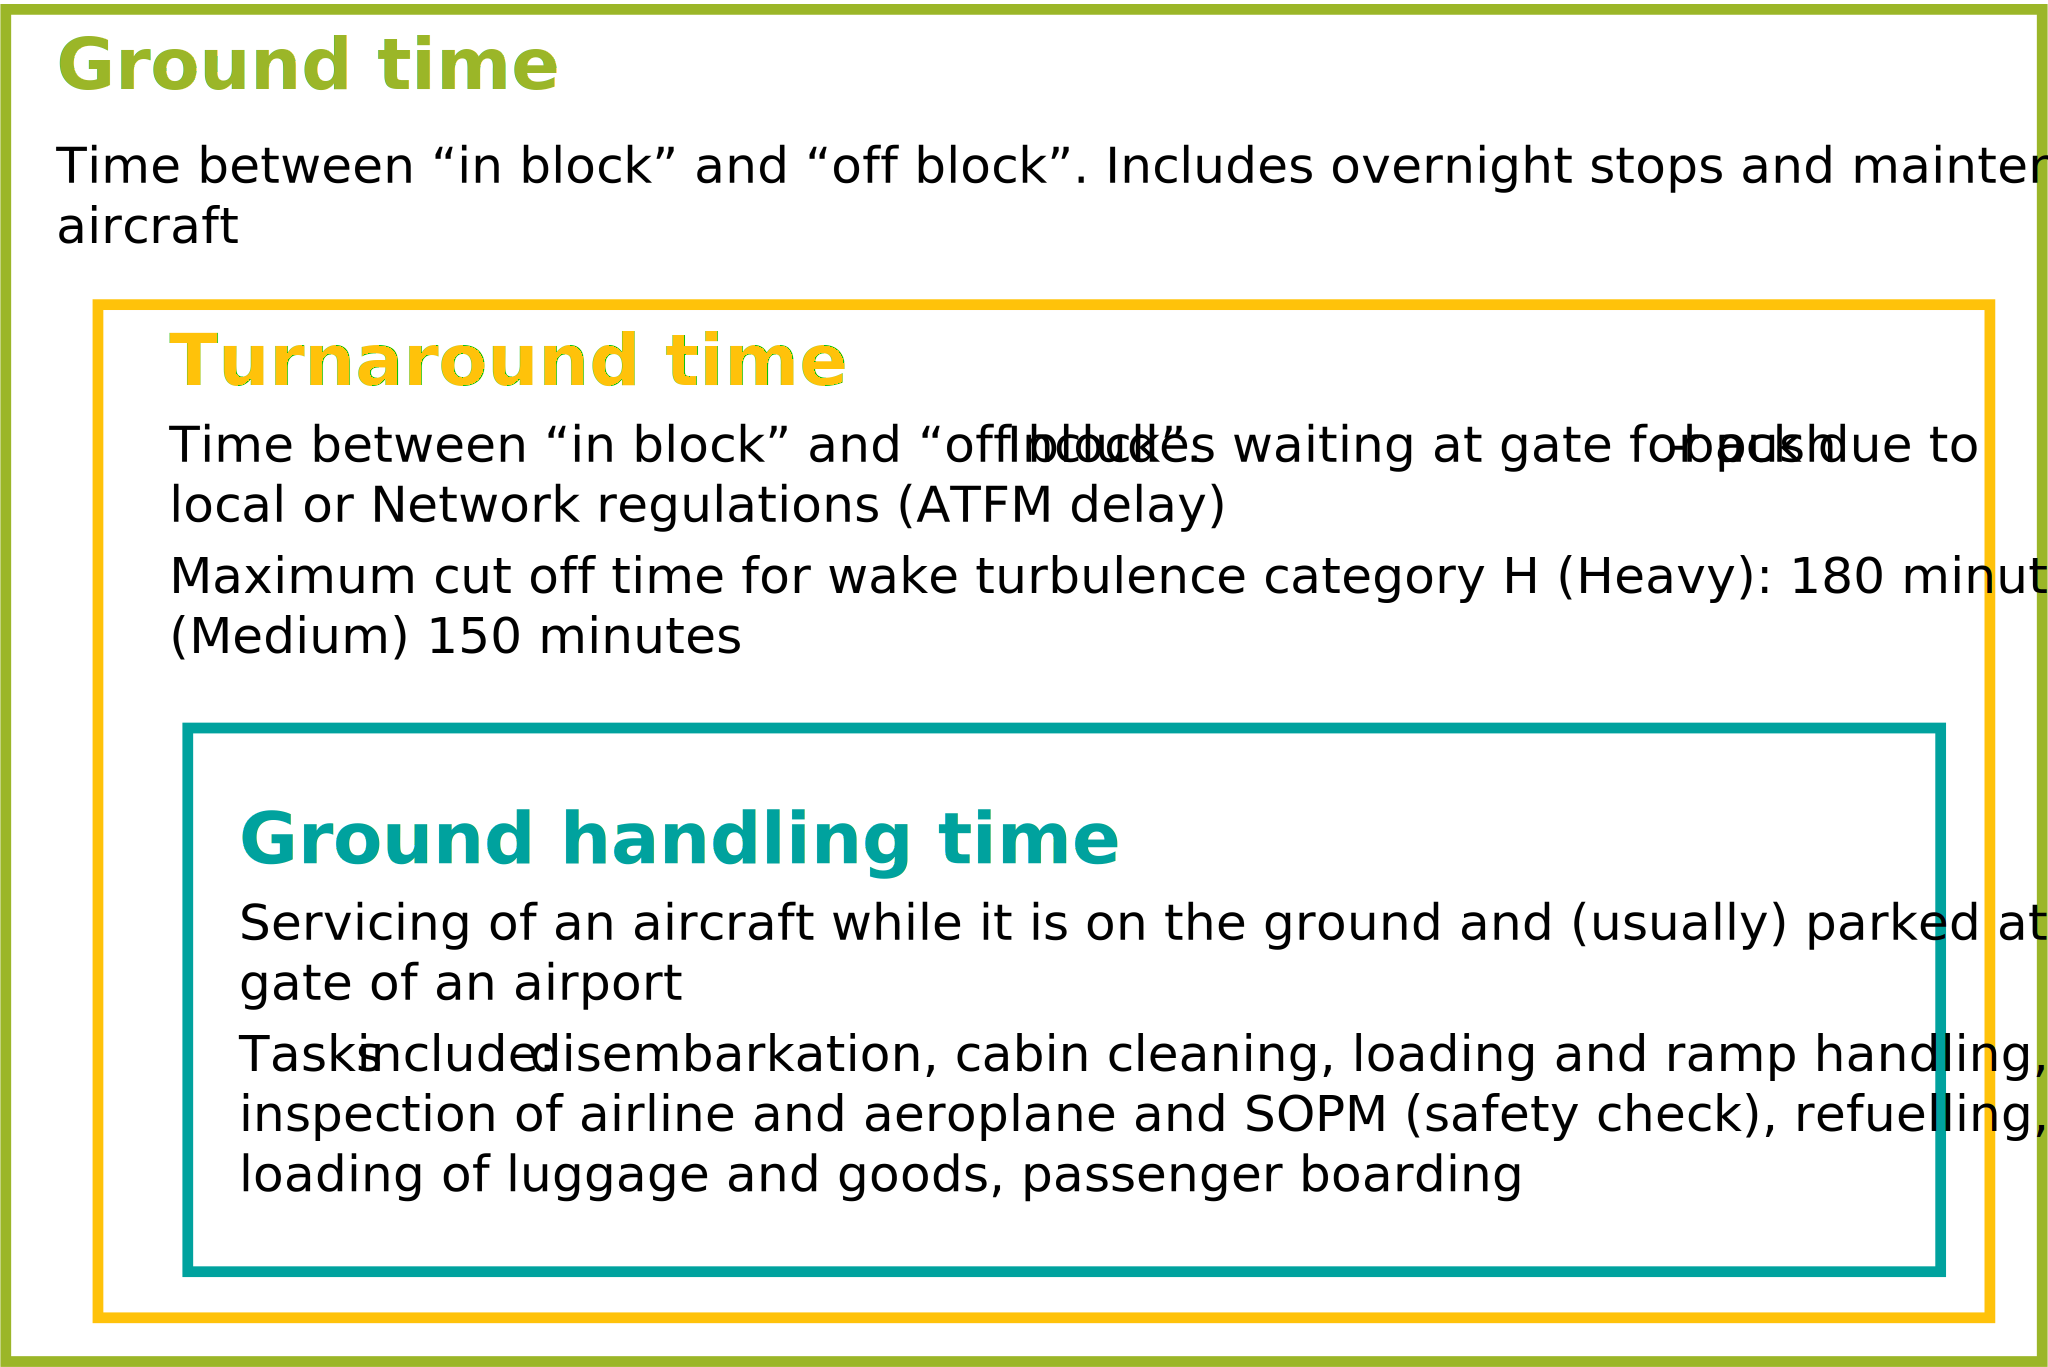
\includegraphics{chapters/../figures/turnaround_activities.svg}

}

\caption{\label{fig-turnaround-activities}Overview of activities
involved in turnaround process}

\end{figure}

\hypertarget{related-inputs-13}{%
\section{Related inputs}\label{related-inputs-13}}

Chapter~\ref{sec-airport-classification}
\protect\hyperlink{sec-airport-classification}{Airport classification}

\hypertarget{references-17}{%
\section{References}\label{references-17}}

\hypertarget{sec-if-average-flight-distance-and-flight-duration}{%
\chapter{IFR average flight distance and flight
duration}\label{sec-if-average-flight-distance-and-flight-duration}}

\hypertarget{eurocontrol-recommended-values-16}{%
\section{EUROCONTROL recommended
values}\label{eurocontrol-recommended-values-16}}

Table~\ref{tbl-flight-distance} presents an overview of the average
flight distance in ECAC region, as well as the average flight time in
the same region for the period 2017-2021.

The data in Table~\ref{tbl-flight-distance} was obtained by dividing the
total distance actually flown and the total yearly IFR flight hours
respectively by the yearly number of IFR flights in the ECAC
airspace.\protect\hyperlink{ref-ectrlprr2021}{{[}42{]}}
\protect\hyperlink{ref-ectrlprr2022}{{[}43{]}}
\protect\hyperlink{ref-ectrl:statfor:sid}{{[}5{]}}

Please note that the numbers for 2020 and 2021 are considerably lower
due to the effect of pandemic.

\hypertarget{tbl-flight-distance}{}
\setlength{\LTpost}{0mm}
\begin{longtable}{lrrr}
\caption{\label{tbl-flight-distance}Average IFR flight distance and duration in ECAC }\tabularnewline

\toprule
Year & Distance in km & Distance in NM & Flight time in min \\ 
\midrule
2017 & $1,197$ & $646.00$ & $98.40$ \\ 
2018 & $1,209$ & $653.00$ & $100.10$ \\ 
2019 & $1,220$ & $659.00$ & $101.30$ \\ 
2020 & $510$ & $275.00$ & $97.50$ \\ 
2021 & $661$ & $357.00$ & $1,000.00$ \\ 
\bottomrule
\end{longtable}
\begin{minipage}{\linewidth}
\emph{Source: \href{https://www.eurocontrol.int/publication/performance-review-report-prr-2021}{EUROCONTROL (2022) Performance Review Report (PRR) 2021}; \href{https://www.eurocontrol.int/publication/performance-review-report-prr-2020}{EUROCONTROL (2022) Performance Review Report (PRR) 2020}; \href{https://ext.eurocontrol.int/analytics/saw.dll?Dashboard}{STATFOR Interactive Dashboard}}\\
\end{minipage}

With regard to flight distance,
Figure~\ref{fig-traffic-demand-distribution} illustrates that nearly
90\% of IFR flight distances for flights arriving or departing within
the Network Manager area (excl. overflights) are less than 1,000NM long.

\begin{figure}

{\centering 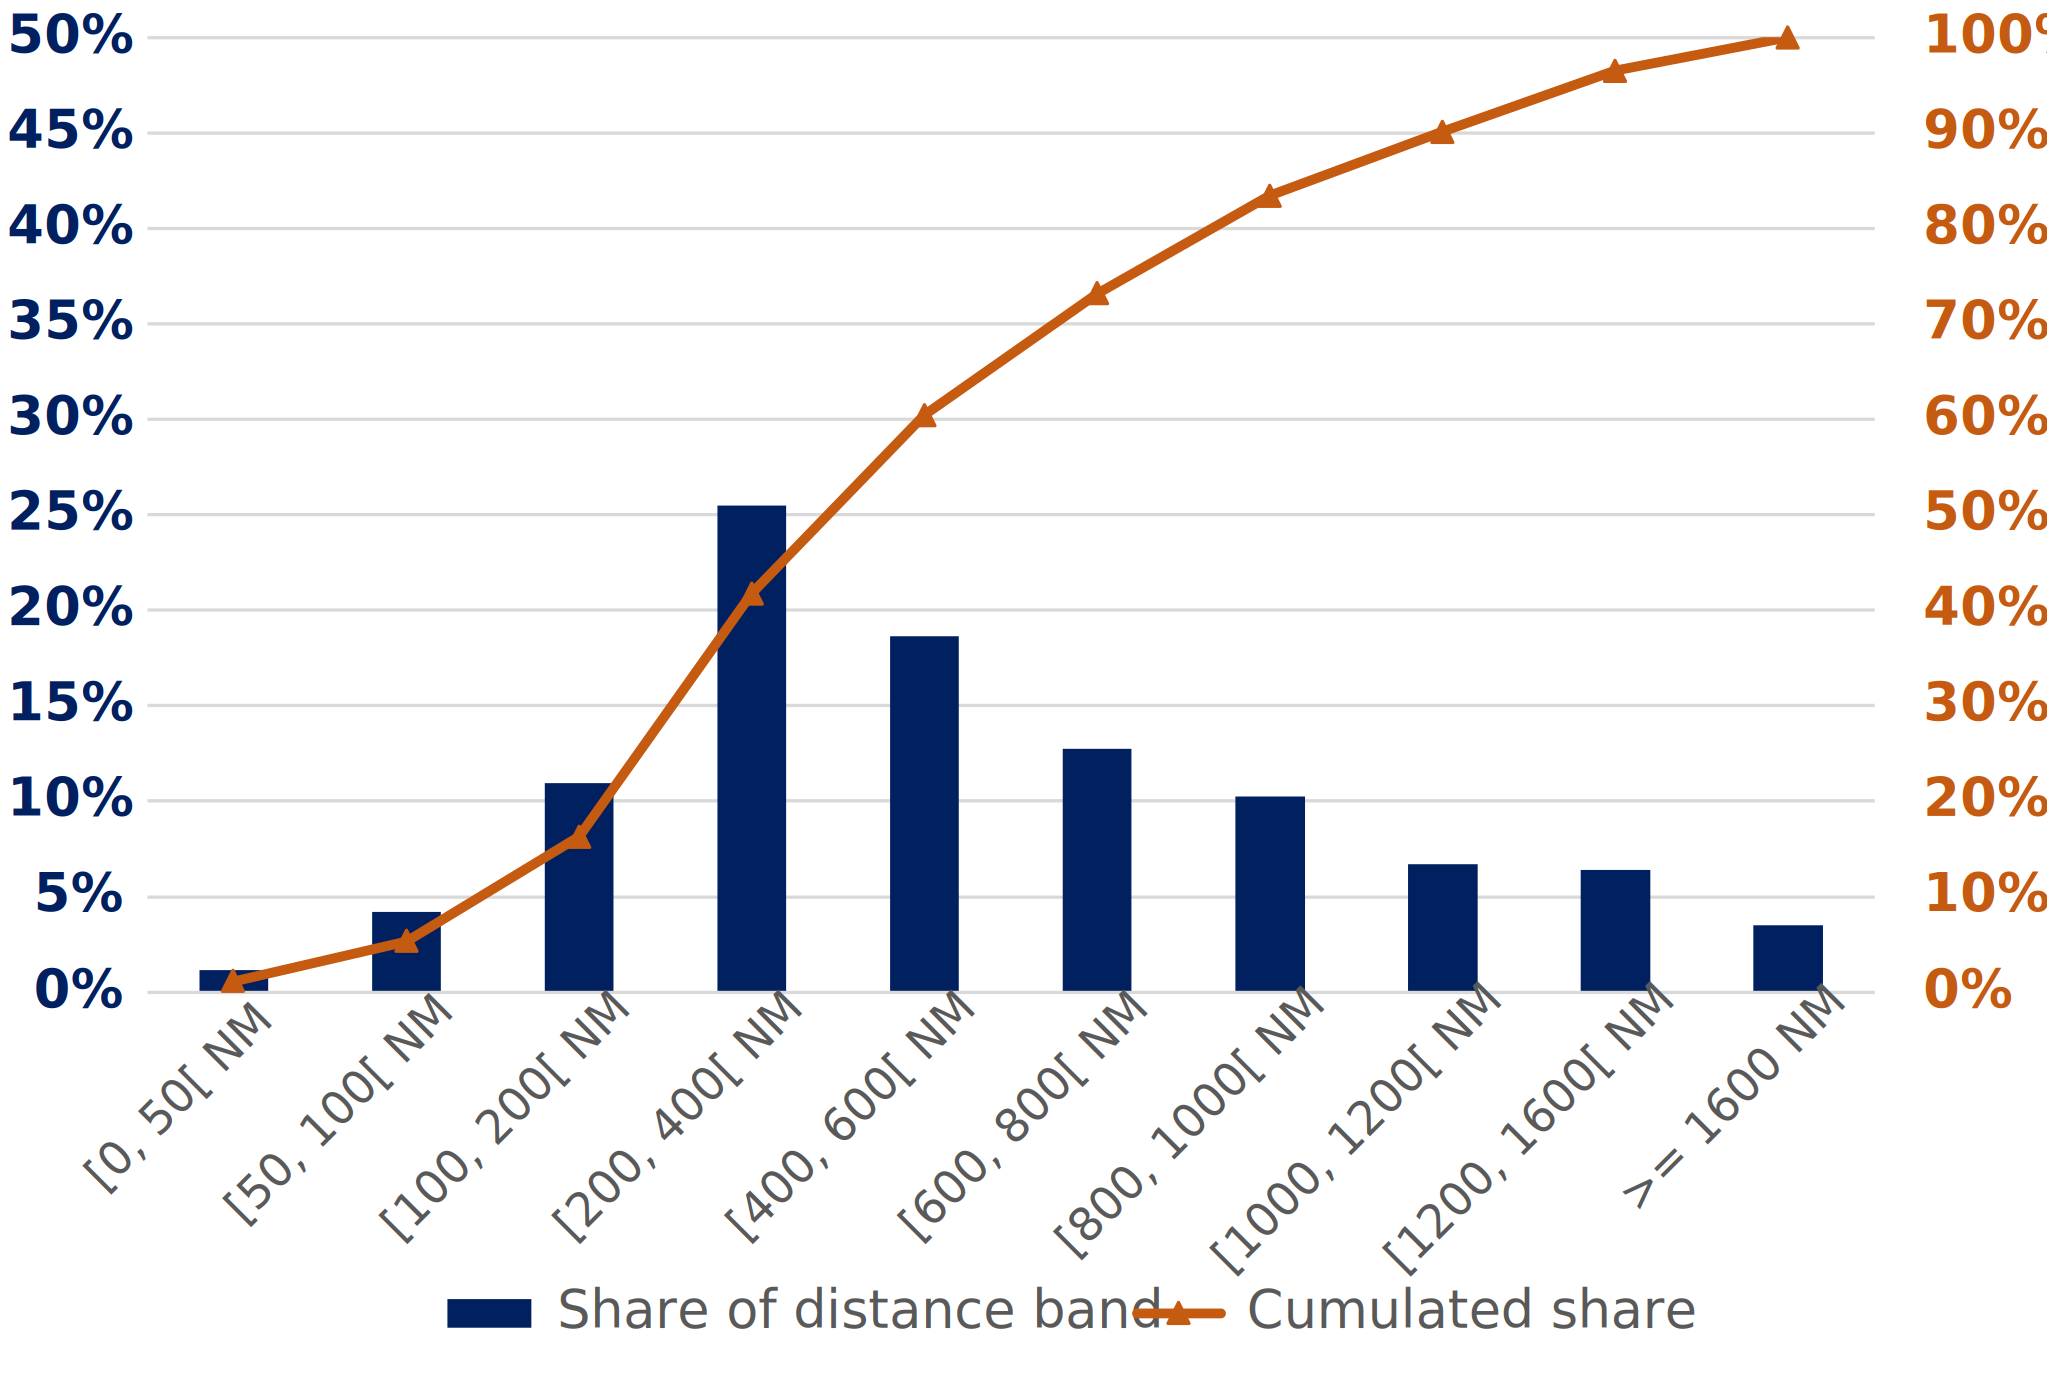
\includegraphics{chapters/../figures/traffic_demand_distribution.svg}

}

\caption{\label{fig-traffic-demand-distribution}Distribution of traffic
demand per distance band in 2022 within the EUROCONTROL Network Manager
area}

\end{figure}

\hypertarget{related-inputs-14}{%
\section{Related inputs}\label{related-inputs-14}}

Chapter~\ref{sec-ifr-flight-information-per-market-segment}
\protect\hyperlink{sec-ifr-flight-information-per-market-segment}{IFR
flight information per market segment}

Chapter~\ref{sec-distance-flown-by-charging-zone}
\protect\hyperlink{sec-distance-flown-by-charging-zone}{DIstance flown
by charging zone}

Chapter~\ref{sec-taxiing-time}
\protect\hyperlink{sec-taxiing-time}{Taxiing time}

\hypertarget{references-18}{%
\section{References}\label{references-18}}

\hypertarget{sec-ifr-flight-information-per-market-segment}{%
\chapter{IFR flight information per market
segment}\label{sec-ifr-flight-information-per-market-segment}}

\hypertarget{eurocontrol-recommended-values-17}{%
\section{EUROCONTROL recommended
values}\label{eurocontrol-recommended-values-17}}

Table~\ref{tbl-ifr-info} shows the mean distance, fuel consumption and
flight duration of an IFR flight, per market segment,\footnote{\href{https://www.eurocontrol.int/publication/market-segment-rules}{Rules
  for the EUROCONTROL classification of low-cost, all-cargo and business
  aviation types of flights}} in ECAC region. These values refer to year
2019.

\hypertarget{tbl-ifr-info}{}
\setlength{\LTpost}{0mm}
\begin{longtable}{lrrrr}
\caption{\label{tbl-ifr-info}Average IFR flight values per market segment }\tabularnewline

\toprule
Market segment & Number of IFR flights & Average flight distance (NM) & Average flight duration (min) & Average fuel burn (kg) \\ 
\midrule
\multicolumn{5}{l}{Flights within ECAC} \\ 
\midrule
Traditional scheduled & $4,077,653$ & $470$ & $99$ & $3,366$ \\ 
Low-cost & $3,098,905$ & $676$ & $126$ & $4,672$ \\ 
Business aviation & $568,530$ & $390$ & $91$ & $901$ \\ 
Non-scheduled charter & $249,413$ & $684$ & $130$ & $4,370$ \\ 
Other types & $242,793$ & $197$ & $88$ & $560$ \\ 
All cargo & $217,620$ & $460$ & $99$ & $5,794$ \\ 
Total & $8,454,914$ & $538$ & $109$ & $3,691$ \\ 
\midrule
\multicolumn{5}{l}{International flights entering and leaving ECAC} \\ 
\midrule
Traditional scheduled & $1,608,581$ & $2,706$ & $384$ & $39,109$ \\ 
Low-cost & $243,398$ & $1,716$ & $260$ & $14,679$ \\ 
Business aviation & $151,540$ & $1,527$ & $238$ & $13,782$ \\ 
Non-scheduled charter & $94,738$ & $2,709$ & $377$ & $34,981$ \\ 
Other types & $94,514$ & $2,682$ & $383$ & $36,145$ \\ 
All cargo & $7,679$ & $1,862$ & $293$ & $21,150$ \\ 
Total & $2,200,450$ & $2,511$ & $360$ & $34,295$ \\ 
\bottomrule
\end{longtable}
\begin{minipage}{\linewidth}
\emph{Source: EUROCONTROL -- derived from an analysis of 2019 IFR flights carried out in Europe (excluding overflights) and calculated by AEM, BADA tabulated}\\
\end{minipage}

\hypertarget{description-7}{%
\section{Description}\label{description-7}}

The calculations were made on the basis of:

\begin{itemize}
\item
  2019 full year total distance and ECAC distance flown, extracted from
  data collected by the Network Manager, not including overflights
\item
  the EUROCONTROL Small Emitters Tool (SET) approved by the European
  Commission by Commission Regulation (EU) No 606/2010
\item
  use of the latest version of the BADA
  \protect\hyperlink{ref-ectl:bada}{{[}44{]}} tabulated model 4 and AEM
  (Advanced Emission Model)
\item
  fuel burn figures, not taking into account the reduction in the
  aircraft's weight in fuel during the flight
\end{itemize}

\hypertarget{related-inputs-15}{%
\section{Related inputs}\label{related-inputs-15}}

Chapter~\ref{sec-number-of-ifr-flights}
\protect\hyperlink{sec-number-of-ifr-flights}{Number of IFR flights}

Chapter~\ref{sec-rate-of-fuel-burn}
\protect\hyperlink{sec-rate-of-fuel-burn}{Rate of fuel burn}

Chapter~\ref{sec-amount-of-emissions-released-by-fuel-burn}
\protect\hyperlink{sec-amount-of-emissions-released-by-fuel-burn}{Amount
of emissions released by fuel burn}

Chapter~\ref{sec-cost-of-emissions}
\protect\hyperlink{sec-cost-of-emissions}{Cost of emissions}

Chapter~\ref{sec-if-average-flight-distance-and-flight-duration}
\protect\hyperlink{sec-if-average-flight-distance-and-flight-duration}{IFR
average flight distance and flight duration}

Chapter~\ref{sec-fleet-size} \protect\hyperlink{sec-fleet-size}{Fleet
size}

Chapter~\ref{sec-taxiing-time}
\protect\hyperlink{sec-taxiing-time}{Taxiing time}

\hypertarget{references-19}{%
\section{References}\label{references-19}}

\hypertarget{sec-distance-flown-by-charging-zone}{%
\chapter{Distance flown by charging
zone}\label{sec-distance-flown-by-charging-zone}}

\hypertarget{eurocontrol-recommended-values-18}{%
\section{EUROCONTROL recommended
values}\label{eurocontrol-recommended-values-18}}

Table~\ref{tbl-distance-flown} below shows the million of kilometers
flown by charging zone.\protect\hyperlink{ref-ace2020}{{[}45{]}}

\hypertarget{tbl-distance-flown}{}
\setlength{\LTpost}{0mm}
\begin{longtable}{lrrrrrrrrr}
\caption{\label{tbl-distance-flown}Distance flown by charging zone in M km }\tabularnewline

\toprule
State & 2014 & 2015 & 2016 & 2017 & 2018 & 2019 & 2020 & 2021 & 2022 \\ 
\midrule
Albania & $33$ & $34$ & $31$ & $32$ & $34$ & $36$ & $16$ & $24$ & $38$ \\ 
Armenia & $9$ & $7$ & $7$ & $10$ & $13$ & $12$ & $3$ & $5$ & $11$ \\ 
Austria & $202$ & $204$ & $204$ & $219$ & $235$ & $244$ & $109$ & $135$ & $232$ \\ 
Belgium-Luxembourg & $175$ & $181$ & $183$ & $189$ & $193$ & $187$ & $75$ & $82$ & $149$ \\ 
Bosnia and Herzegovina & $59$ & $64$ & $63$ & $74$ & $79$ & $88$ & $41$ & $55$ & $90$ \\ 
Bulgaria & $174$ & $201$ & $205$ & $208$ & $233$ & $236$ & $101$ & $139$ & $231$ \\ 
Croatia & $131$ & $133$ & $131$ & $134$ & $148$ & $161$ & $66$ & $110$ & $164$ \\ 
Cyprus & $104$ & $109$ & $109$ & $123$ & $136$ & $146$ & $56$ & $84$ & $122$ \\ 
Czech Republic & $167$ & $177$ & $189$ & $193$ & $208$ & $204$ & $78$ & $90$ & $128$ \\ 
Denmark & $120$ & $123$ & $125$ & $127$ & $130$ & $133$ & $52$ & $56$ & $99$ \\ 
Finland & $58$ & $55$ & $54$ & $59$ & $65$ & $68$ & $31$ & $32$ & $46$ \\ 
France & $1,489$ & $1,514$ & $1,594$ & $1,673$ & $1,714$ & $1,729$ & $689$ & $902$ & $1,506$ \\ 
Georgia & $40$ & $41$ & $41$ & $42$ & $42$ & $37$ & $20$ & $23$ & $41$ \\ 
Germany & $990$ & $994$ & $1,029$ & $1,087$ & $1,130$ & $1,137$ & $505$ & $578$ & $951$ \\ 
Greece & $332$ & $344$ & $328$ & $364$ & $401$ & $426$ & $182$ & $275$ & $447$ \\ 
Hungary & $158$ & $173$ & $178$ & $189$ & $207$ & $202$ & $89$ & $114$ & $201$ \\ 
Ireland & $197$ & $209$ & $224$ & $224$ & $226$ & $228$ & $95$ & $115$ & $209$ \\ 
Italy & $671$ & $660$ & $671$ & $697$ & $753$ & $796$ & $321$ & $467$ & $757$ \\ 
Latvia & $54$ & $55$ & $54$ & $59$ & $63$ & $64$ & $27$ & $33$ & $34$ \\ 
Lithuania & $36$ & $35$ & $36$ & $39$ & $44$ & $45$ & $22$ & $31$ & $29$ \\ 
Malta & $41$ & $46$ & $49$ & $50$ & $52$ & $57$ & $23$ & $28$ & $38$ \\ 
Moldova & $9$ & $6$ & $5$ & $6$ & $7$ & $7$ & $3$ & $4$ & $2$ \\ 
Netherlands & $202$ & $213$ & $226$ & $232$ & $242$ & $240$ & $101$ & $106$ & $188$ \\ 
North Macedonia & $19$ & $20$ & $19$ & $23$ & $26$ & $30$ & $12$ & $20$ & $31$ \\ 
Norway & $172$ & $173$ & $181$ & $182$ & $183$ & $177$ & $94$ & $108$ & $158$ \\ 
Poland & $289$ & $288$ & $306$ & $316$ & $344$ & $360$ & $148$ & $183$ & $237$ \\ 
Portugal Lisboa & $216$ & $226$ & $252$ & $272$ & $277$ & $287$ & $112$ & $144$ & $266$ \\ 
Portugal Santa Maria & $196$ & $217$ & $236$ & $251$ & $259$ & $260$ & $117$ & $143$ & $243$ \\ 
Romania & $251$ & $266$ & $257$ & $274$ & $298$ & $299$ & $126$ & $175$ & $276$ \\ 
Serbia / Montenegro / KFOR & $133$ & $149$ & $158$ & $166$ & $186$ & $195$ & $83$ & $113$ & $194$ \\ 
Slovak Republic & $72$ & $72$ & $76$ & $79$ & $86$ & $86$ & $31$ & $41$ & $65$ \\ 
Slovenia & $37$ & $37$ & $39$ & $41$ & $44$ & $48$ & $20$ & $28$ & $45$ \\ 
Spain-Canarias & $101$ & $98$ & $106$ & $114$ & $124$ & $131$ & $356$ & $73$ & $124$ \\ 
Spain-Continental & $707$ & $725$ & $780$ & $835$ & $881$ & $909$ & $57$ & $512$ & $875$ \\ 
Sweden & $257$ & $258$ & $261$ & $276$ & $287$ & $283$ & $120$ & $129$ & $199$ \\ 
Switzerland & $120$ & $121$ & $124$ & $134$ & $144$ & $144$ & $54$ & $75$ & $127$ \\ 
Turkey & $789$ & $856$ & $853$ & $933$ & $1,021$ & $1,036$ & $460$ & $658$ & $938$ \\ 
United Kingdom & $706$ & $720$ & $768$ & $821$ & $838$ & $852$ & $335$ & $360$ & $719$ \\ 
Subtotal & $9,516$ & $9,805$ & $10,153$ & $10,748$ & $11,352$ & $11,582$ & $4,829$ & $6,250$ & $10,208$ \\ 
Estonia\textsuperscript{1} & NA & NA & NA & $41$ & $56$ & $55$ & $23$ & $26$ & $29$ \\ 
Ukraine\textsuperscript{2} & NA & NA & NA & NA & NA & NA & NA & NA & $12$ \\ 
Ukraine south & NA & NA & NA & NA & NA & NA & NA & NA & $2$ \\ 
Total & $9,516$ & $9,805$ & $10,153$ & $10,789$ & $11,407$ & $11,636$ & $4,853$ & $6,279$ & $10,239$ \\ 
\bottomrule
\end{longtable}
\begin{minipage}{\linewidth}
\textsuperscript{1}Estonia integrated as of April 2017\\
\textsuperscript{2}Ukraine integrated as of November 2021\\
\emph{Source: \href{https://ansperformance.eu/publications/prc/ace/}{EUROCONTROL PRU (2022), Air traffic management cost-effectiveness (ACE) benchmarking report for 2020 with 2021-2024 outlook}}\\
\end{minipage}

For the most updated information, please refer to the
\href{https://www.eurocontrol.int/ServiceUnits/Dashboard/EnRouteMainDashboard.html}{Aviation
Intelligence En-Route Dashboard}.

\hypertarget{description-8}{%
\section{Description}\label{description-8}}

The Report on the Operation of the Route Charges System is published by
the CRCO on an annual basis and provides data on traffic volumes and ATM
costs for the States for which the CRCO collects en route and terminal
charges.

Table~\ref{tbl-distance-flown} sets out the number of millions of
kilometres recorded in the airspace of the Contracting States from 2014
to 2022 for the calculation of route charges (great circle distance
after deduction of 20 km for departing and arriving flights) .

Information on the various different charges levied by the CRCO, in
particular the charge calculation methods, the basic billing documents,
the methods of payment and the submission of claims is described in
\href{https://www.eurocontrol.int/publication/customer-guide-route-charges}{``Customer
Guide to Charges''}.

\hypertarget{related-inputs-16}{%
\section{Related inputs}\label{related-inputs-16}}

Chapter~\ref{sec-if-average-flight-distance-and-flight-duration}
\protect\hyperlink{sec-if-average-flight-distance-and-flight-duration}{IFR
average flight distance and flight duration}

Chapter~\ref{sec-en-route-ans-costs}
\protect\hyperlink{sec-en-route-ans-costs}{En-route ANS costs}

Chapter~\ref{sec-route-charge-share-per-market-segment}
\href{sec-route-charge-share-per-market-segment}{Route charge share per
market segment}

\hypertarget{references-20}{%
\section{References}\label{references-20}}

\hypertarget{sec-load-factor-cargo}{%
\chapter{Load factor -- cargo}\label{sec-load-factor-cargo}}

\hypertarget{eurocontrol-recommended-values-19}{%
\section{EUROCONTROL recommended
values}\label{eurocontrol-recommended-values-19}}

The value below presents the percentage of cargo space in flights filled
by paid cargo.

\hypertarget{tbl-load-pax-iata}{}
\setlength{\LTpost}{0mm}
\begin{longtable}{lc}
\caption{\label{tbl-load-pax-iata}Passenger load factor -- IATA values }\tabularnewline

\toprule
Year & Load factor\textsuperscript{1} \\ 
\midrule
2017 & $46.40\%$ \\ 
2018 & $54.30\%$ \\ 
2019 & $51.70\%$ \\ 
2020 & $59.70\%$ \\ 
2021 & $67.20\%$ \\ 
2022 & $56.70\%$ \\ 
\bottomrule
\end{longtable}
\begin{minipage}{\linewidth}
\textsuperscript{1}The values used in this table come from IATA monthly Air Freight Market Analysis reports for the month of December of each year. The data is extracted from the table “Air freight market detail”, looking at Total market in Europe, column CLF(level) for calendar year.\\
\emph{Source: IATA -- Economics, Air Freight Market Analysis for December 2017-2022. Available at \href{https://www.iata.org/en/publications/economics/?page=14\&Search=Air\%20Passenger\%20Market\%20Analysis\%20-\%20December\%20\&Year=2023\&Year=2022\&Year=2021\&Year=2020\&Ordering=DateDesc}{IATA Economics}}\\
\end{minipage}

Cargo flights can be defined here as either freight carriers or
passenger/cargo carriers. Note that geographical coverage of IATA Europe
covers ECAC States and other countries, including Russia, Tajikistan,
Turkmenistan and Uzbekistan.

\hypertarget{sec-load-factor-passengers}{%
\chapter{Load factor -- passengers}\label{sec-load-factor-passengers}}

\hypertarget{eurocontrol-recommended-values-20}{%
\section{EUROCONTROL recommended
values}\label{eurocontrol-recommended-values-20}}

The load factor represents the percentage of seats filled by fare paying
passengers on a flight.

Table~\ref{tbl-load-pax-statfor} shows the estimated passenger load
factor according to EUROCONTROL STATFOR values. These values were
obtained by dividing the total number of passengers by the total number
of available seats on the flights. This information is based on the data
produced by Eurostat and covers the EU27+UK, and four EFTA
states.\footnote{European Free Trade Association: Iceland,
  Liechtenstein, Norway and Switzerland}

\hypertarget{tbl-load-pax-statfor}{}
\setlength{\LTpost}{0mm}
\begin{longtable}{lc}
\caption{\label{tbl-load-pax-statfor}Passenger load factor -- EUROCONTROL values }\tabularnewline

\toprule
Year & Load factor \\ 
\midrule
2017 & $82.60\%$ \\ 
2018 & $82.60\%$ \\ 
2019 & $83.30\%$ \\ 
2020 & $59.40\%$ \\ 
2021 & $65.30\%$ \\ 
\bottomrule
\end{longtable}
\begin{minipage}{\linewidth}
\emph{Source: \href{https://www.eurocontrol.int/dashboard/statfor-interactive-dashboard}{EUROCONTROL STATFOR Interactive Dashboard (PAX+)}}\\
\end{minipage}

Table~\ref{tbl-load-pax-iata} presents the evolution in the passenger
load factor according to IATA data. These values represent the ratio of
revenue passenger km to available seat km. The difference from values in
Table 1 is the geographical coverage: IATA's Europe area is larger than
EU Europe statistical area, it also covers countries such as Russia,
Tajikistan, Turkmenistan and Uzbekistan.

\hypertarget{tbl-load-pax-iata}{}
\setlength{\LTpost}{0mm}
\begin{longtable}{lc}
\caption{\label{tbl-load-pax-iata}Passenger load factor -- IATA values }\tabularnewline

\toprule
Year & Load factor\textsuperscript{1} \\ 
\midrule
2017 & $83.90\%$ \\ 
2018 & $84.50\%$ \\ 
2019 & $85.20\%$ \\ 
2020 & $67.80\%$ \\ 
2021 & $74.50\%$ \\ 
2022 & $83.60\%$ \\ 
\bottomrule
\end{longtable}
\begin{minipage}{\linewidth}
\textsuperscript{1}The values used in this table come from IATA monthly Air Passenger Market Analysis reports for the month of December of each year. The data is extracted from the table “Air passenger market detail”, looking at Total market in Europe, column PLF(level) for calendar year.\\
\emph{Source: IATA -- Economics, Air Passenger Market Analysis for December 2017-2022. Available at \href{https://www.iata.org/en/publications/economics/?page=14\&Search=Air\%20Passenger\%20Market\%20Analysis\%20-\%20December\%20\&Year=2023\&Year=2022\&Year=2021\&Year=2020\&Ordering=DateDesc}{IATA - Economics}}\\
\end{minipage}

A wide range of economic reports from IATA can be accessed on
\href{https://www.iata.org/en/publications/economics}{IATA website}

\hypertarget{sec-cost-of-aviation-fuel}{%
\chapter{Cost of aviation fuel}\label{sec-cost-of-aviation-fuel}}

\hypertarget{eurocontrol-recommended-sources-1}{%
\section{EUROCONTROL recommended
sources}\label{eurocontrol-recommended-sources-1}}

The source recommended to consult for the latest data on the cost of
aviation fuel is
\href{https://eurocontrol.sharepoint.com/sites/ECTL-Business_Cases/Shared\%20Documents/Standard_Inputs/1.\%20NEW_2022/Values/Cost\%20of\%20aviation\%20fuel/IATA\%20Jet\%20Fuel\%20Price\%20Monitor}{IATA
Jet Fuel Price Monitor}.

On its website, IATA provides jet fuel prices for the major regions of
the world, together with analysis and commentary. The values are based
on \href{http://www.platts.com/}{Platts Energy Market Data}.

When estimating the jet fuel price, consideration should be given to the
selection of the geographical area, and hence currency, as a change in
oil price can have a different effect on the jet fuel price owing to
currency fluctuations, e.g.~the downturn in the euro in 2015.

The `spread' between the aviation fuel price and the underlying oil
price covers the cost of refining, but it can vary significantly with
time depending on underlying demand (e.g.~from consumers needing a
similar fraction to aviation), and on supply problems (such as a
breakdown at a refinery or increasing local prices relative to oil).

\hypertarget{other-possible-sources-2}{%
\section{Other possible sources}\label{other-possible-sources-2}}

Other sources that may be interesting to consult to estimate the price
of jet fuel include:

\begin{itemize}
\item
  \emph{IATA Airline Industry Economic Performance Report and
  Tables}\protect\hyperlink{ref-iataeconperf}{{[}46{]}}
\item
  \emph{US Energy Information Administration (2022), Annual Energy
  Outlook 2023}\protect\hyperlink{ref-eia2023}{{[}47{]}}
\end{itemize}

\hypertarget{references-21}{%
\section{References}\label{references-21}}

\hypertarget{sec-value-of-an-average-passenger-flight}{%
\chapter{Value of an average passenger
flight}\label{sec-value-of-an-average-passenger-flight}}

\hypertarget{eurocontrol-recommended-values-21}{%
\section{EUROCONTROL recommended
values}\label{eurocontrol-recommended-values-21}}

This value represents the monetised benefits of an average passenger
flight in EU27.\footnote{\href{https://ec.europa.eu/eurostat/statistics-explained/index.php/Glossary:EU_enlargements}{EU27
  in 2013}} The values were adjusted to 2022 price levels based on
inflation.

\hypertarget{tbl-value-passenger-flight}{}
\setlength{\LTpost}{0mm}
\begin{longtable}{lrr}
\caption{\label{tbl-value-passenger-flight}Value of an average passenger flight }\tabularnewline

\toprule
  & International flight & Domestic flight \\ 
\midrule
Consumer benefits per flight & $\text{EUR}27,636$ & $\text{EUR}5,070$ \\ 
Airline benefits per flight (excl. fuel and labour) & $\text{EUR}829$ & $\text{EUR}149$ \\ 
Other producer benefits per flight (excl. fuel and labour)\textsuperscript{1} & $\text{EUR}1,493$ & $\text{EUR}739$ \\ 
\bottomrule
\end{longtable}
\begin{minipage}{\linewidth}
\textsuperscript{1}Other producers along the air transport value chain are airports, ANSPs, manufacturers, lessors, GDS/CRSs, travel agents, ground services, catering and maintenance\\
\emph{Source: \href{https://www.iata.org/en/iata-repository/publications/economic-reports/value-of-an-average-passenger-flight-in-eu-27/}{IATA (2013), Economic Briefing - The value of an average passenger flight in the EU27}}\\
\end{minipage}

There is no commonly accepted standard for the value of a flight. The
value will vary over time and between routes and whether it is an
additional frequency on an existing route or a new connection. The
COVID-19 pandemic will most probably change the overall picture. This
should be taken into account when the above values are used.

The values quoted above are the result of a study on the benefits in
monetary value of an average passenger flight in the
EU27.\protect\hyperlink{ref-IATAEconomicBriefing}{{[}48{]}}

IATA, in its briefing note, assesses the economic benefits of an average
scheduled passenger flight from the perspective of the consumer,
producers and the economy as a whole. Its approach to the various
benefits is outlined below.

\textbf{Consumer benefits} are the benefits to passengers in the EU
market. Most passengers value air services more than their expenditure.
The difference between the consumer's willingness to pay (or the gross
consumer benefit) and the price paid constitutes the net consumer
benefit.

\textbf{Producer benefits} are assessed from an investor perspective.
Investors will measure profitability by what that profit represents as a
return on invested capital (ROIC). That return is calculated before
payments of debt interest and shows the earnings available to pay both
debt and equity investors.

This analysis draws on earlier work undertaken by McKinsey \& Company
for IATA on profitability and the air transport value chain, which
calculates the global return on invested capital over the last business
cycle 2004 2011 . The calculated global return on invested capital for
each sector in the value chain is based on sample data and represents
actual returns earned rather than required and/or desired
returns.\footnote{IATA does not endorse the use of the estimated rates
  of return on invested capital for purposes of economic regulation or
  for determining the appropriate or desirable rate of return on
  invested capital. The figures used are based on a global assessment of
  the actual prevailing returns on invested capital in the air transport
  value chain}

On the basis of these figures, the share of producer net benefits
accrued in the EU27 is estimated.\footnote{The allocation of producer
  benefits for airports, GDS/CRS, and travel agents is based on the
  share of global passengers flown either domestically (6\%) or
  internationally (18\%) from and within the EU-27. This approach treats
  domestic and international passengers equally in their contribution to
  the producer benefit. The allocation of producer benefits for
  airlines, ANSPs, manufactures, lessors, ground services, catering, and
  maintenance is based on the share of global available seat kilometres
  flown either domestically (2\%) or internationally (19\%) from and
  within the EU27. These approaches do not account for structural
  differences which may exist between the EU and other regions.
  Nevertheless, these approaches provide a relevant estimation, because
  they are less prone to short- and medium-term shocks such as natural
  disasters and macroeconomic crises, which can create temporary
  distortions in the value chain.}

On top of this, there are also some \textbf{wider economic benefits},
which are the benefits to the wider economy, which go beyond the direct
users of air transport. They may include spill over impacts in and
across economies as a result of increased competition and more efficient
movement of capital and labour.

One of the largest economic benefits of increased connectivity comes
from its impact on the long term productivity of the wider economy.
There are several approaches which may be used to quantify this benefit.
One conservative approach which has been developed, on the basis of the
statistical relationship between air connectivity and labour
productivity, yields an estimate that \textbf{a 10\% rise in
connectivity, relative to a country's GDP, will boost labour
productivity levels by 0.07\%.} The methodology for the analysis is
detailed in IATA's 2007 Aviation Economic Benefits study.
\protect\hyperlink{ref-iata:eco:benefit}{{[}49{]}}

\hypertarget{when-to-use-the-input-7}{%
\section{When to use the input?}\label{when-to-use-the-input-7}}

The use of these values depends on the scope and the viewpoint of the
analysis. For example, an assessment from the point of view of airlines
will focus on the benefits that an additional flight brings to airlines,
whereas an analysis from the perspective of a government or the European
Commission should also include an assessment of benefits for consumers
and the wider economy.

Note also that these values reflect the market conditions and the
passenger demand at the time of the study. For example, changes in
passengers' income, changes in their preferences for air transport or
changes in airlines' market structure can affect these values.

\hypertarget{references-22}{%
\section{References}\label{references-22}}

\hypertarget{sec-fleet-age}{%
\chapter{Fleet age}\label{sec-fleet-age}}

\hypertarget{eurocontrol-recommended-values-22}{%
\section{EUROCONTROL recommended
values}\label{eurocontrol-recommended-values-22}}

The sections below refer to the age of the aircraft operating IFR
flights in Europe.

\hypertarget{age-number-of-aircraft-and-number-of-flights-according-to-the-aircraft-build-year}{%
\subsection{Age, number of aircraft and number of flights according to
the aircraft build
year}\label{age-number-of-aircraft-and-number-of-flights-according-to-the-aircraft-build-year}}

\hypertarget{tbl-fleet-age}{}
\setlength{\LTpost}{0mm}
\begin{longtable}{lrrr}
\caption{\label{tbl-fleet-age}Build year of civil aircraft operating in the EUROCONTROL Network
Manager airspace in Europe in 2022 }\tabularnewline

\toprule
Build Year & Age & Number of aircraft & Flights in 2022 \\ 
\midrule
2022 & 0 & $812$ & $143,326$ \\ 
2021 & 1 & $786$ & $312,504$ \\ 
2020 & 2 & $719$ & $316,766$ \\ 
2019 & 3 & $1,190$ & $526,072$ \\ 
2018 & 4 & $1,207$ & $587,450$ \\ 
2017 & 5 & $1,077$ & $523,181$ \\ 
2016 & 6 & $1,037$ & $583,602$ \\ 
2015 & 7 & $973$ & $437,116$ \\ 
2014 & 8 & $1,037$ & $349,573$ \\ 
2013 & 9 & $884$ & $308,068$ \\ 
2012 & 10 & $876$ & $383,691$ \\ 
2011 & 11 & $807$ & $427,566$ \\ 
2010 & 12 & $889$ & $405,560$ \\ 
2009 & 13 & $869$ & $505,334$ \\ 
2008 & 14 & $970$ & $465,372$ \\ 
2007 & 15 & $896$ & $396,296$ \\ 
2006 & 16 & $721$ & $300,833$ \\ 
2005 & 17 & $511$ & $194,098$ \\ 
2004 & 18 & $405$ & $147,659$ \\ 
2003 & 19 & $395$ & $147,586$ \\ 
2002 & 20 & $439$ & $158,016$ \\ 
2001 & 21 & $548$ & $175,071$ \\ 
2000 & 22 & $519$ & $172,889$ \\ 
1999 & 23 & $479$ & $152,486$ \\ 
1998 & 24 & $411$ & $111,587$ \\ 
1997 & 25 & $256$ & $79,570$ \\ 
1996 & 26 & $248$ & $79,072$ \\ 
1995 & 27 & $155$ & $48,231$ \\ 
1994 & 28 & $192$ & $62,915$ \\ 
1993 & 29 & $204$ & $60,005$ \\ 
1992 & 30 & $245$ & $55,084$ \\ 
1991 & 31 & $187$ & $52,850$ \\ 
1990 & 32 & $160$ & $39,327$ \\ 
1989 & 33 & $135$ & $29,426$ \\ 
1988 & 34 & $104$ & $18,502$ \\ 
1987 & 35 & $68$ & $14,082$ \\ 
1986 & 36 & $74$ & $12,643$ \\ 
1985 & 37 & $49$ & $6,648$ \\ 
1984 & 38 & $68$ & $5,123$ \\ 
1983 & 39 & $34$ & $3,818$ \\ 
1982 & 40 & $92$ & $5,410$ \\ 
before 1982 & > 40 & $894$ & $41,246$ \\ 
unknown & unknown & $301$ & $243,333$ \\ 
Grand Total & NA & $22,923$ & $9,088,987$ \\ 
\bottomrule
\end{longtable}
\begin{minipage}{\linewidth}
\emph{Source: EUROCONTROL Network Manager flight plans and PRISME fleet data, March 2023}\\
\end{minipage}

The information presented in Table~\ref{tbl-fleet-age} is derived from
flight plans submitted to the EUROCONTROL Network Manager (NM) for
flights in 2022. These aircraft were therefore active in European
airspace at some point during that year. The information was analysed
using the EUROCONTROL PRISME fleet database to derive the aircraft ages.

Since the numbers are based on flight plans, they exclude aircraft which
do not fly in controlled airspace and therefore do not submit flight
plans to the NM. The 301 aircraft whose age was unknown were aircraft
which are not recorded in the PRISME database. These are mostly
privately owned aircraft or aircraft based outside Europe, together with
some smaller aircraft not flying regularly in controlled airspace and
some new aircraft which do not feature in the database.

\hypertarget{average-aircraft-age-per-flight-eu27efta}{%
\subsection[Average aircraft age per flight
(EU27+EFTA)]{\texorpdfstring{Average aircraft age per flight
(EU27+EFTA\footnote{European Free Trade Association whose Member States
  comprise Iceland, Liechtenstein, Norway and Switzerland})}{Average aircraft age per flight (EU27+EFTA)}}\label{average-aircraft-age-per-flight-eu27efta}}

Figure~\ref{fig-average-aircraft-age} shows the average aircraft age in
years by EUROCONTROL market
segment\protect\hyperlink{ref-ectl:market:seg:2022}{{[}12{]}} for the
aircraft operating in 2022.

\begin{figure}

{\centering 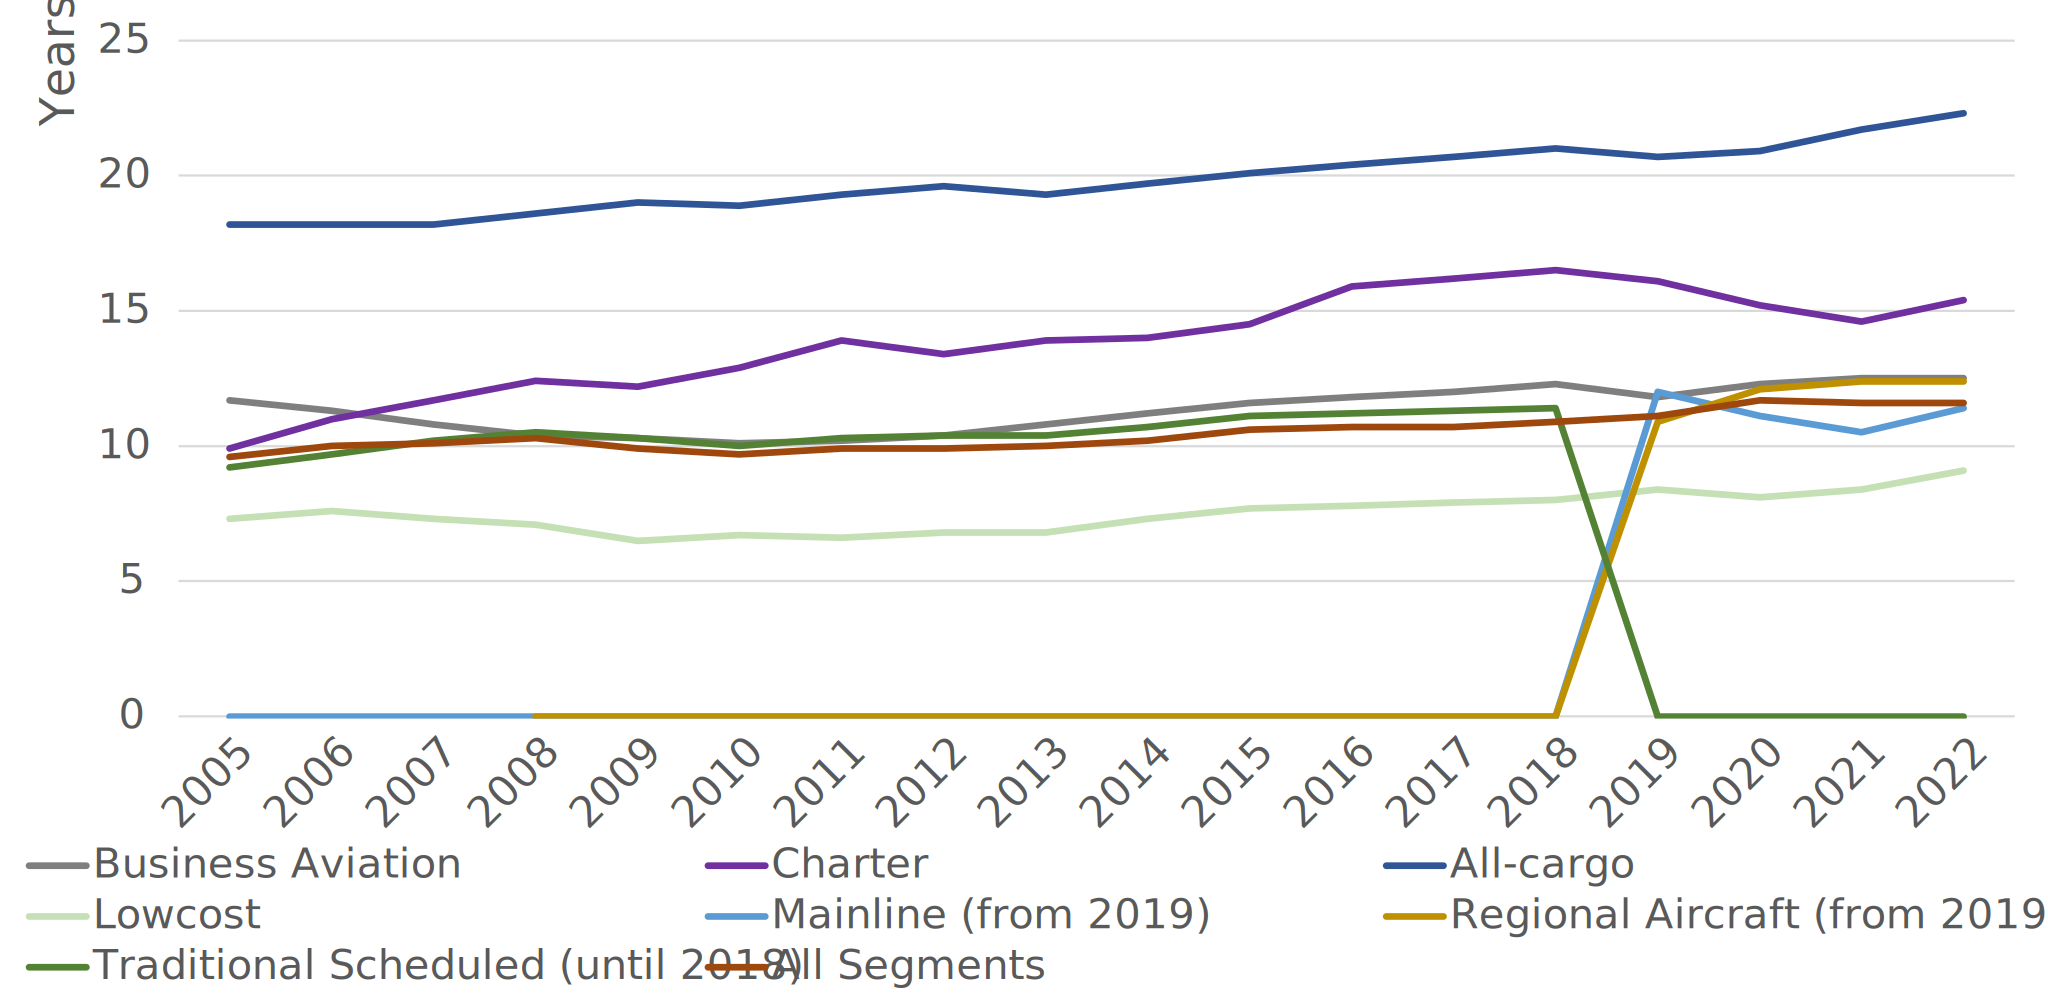
\includegraphics{chapters/../figures/aircraft_age_per_flight.svg}

}

\caption{\label{fig-average-aircraft-age}Average aircraft age per flight
in EU27 + EFTA\protect\hyperlink{ref-ectrl:statfor:sid}{{[}5{]}}}

\end{figure}

\begin{tcolorbox}[enhanced jigsaw, opacityback=0, arc=.35mm, colframe=quarto-callout-note-color-frame, breakable, left=2mm, leftrule=.75mm, titlerule=0mm, colbacktitle=quarto-callout-note-color!10!white, rightrule=.15mm, opacitybacktitle=0.6, bottomtitle=1mm, colback=white, toptitle=1mm, title=\textcolor{quarto-callout-note-color}{\faInfo}\hspace{0.5em}{Note}, bottomrule=.15mm, toprule=.15mm, coltitle=black]

EUROCONTROL market segments were updated in 2022 and saw the
``Traditional Scheduled'' segment split into ``Mainline'' and
``Regional'' according to EUROCONTROL Market Segment
Rules.\protect\hyperlink{ref-ectl:market:seg:2022}{{[}12{]}}

\end{tcolorbox}

Low-cost carriers have the youngest fleet on average, at 9.1 years in
2022, while charter and all-cargo have much older fleets, at 22 years
for all-cargo and 15.4 years for charter flights in 2022. The increase
in market share of all-cargo and business aviation in the aftermath of
the COVID-19 pandemic, has pushed the average age of the overall fleet
up to 11.6 years in 2022.

\hypertarget{commercial-aircraft-fleet-by-age-of-aircraft}{%
\subsection{Commercial aircraft fleet by age of
aircraft}\label{commercial-aircraft-fleet-by-age-of-aircraft}}

Figure~\ref{fig-com-aircraft-fleet} shows the commercial aircraft fleet
size by age of aircraft.

\begin{figure}

{\centering 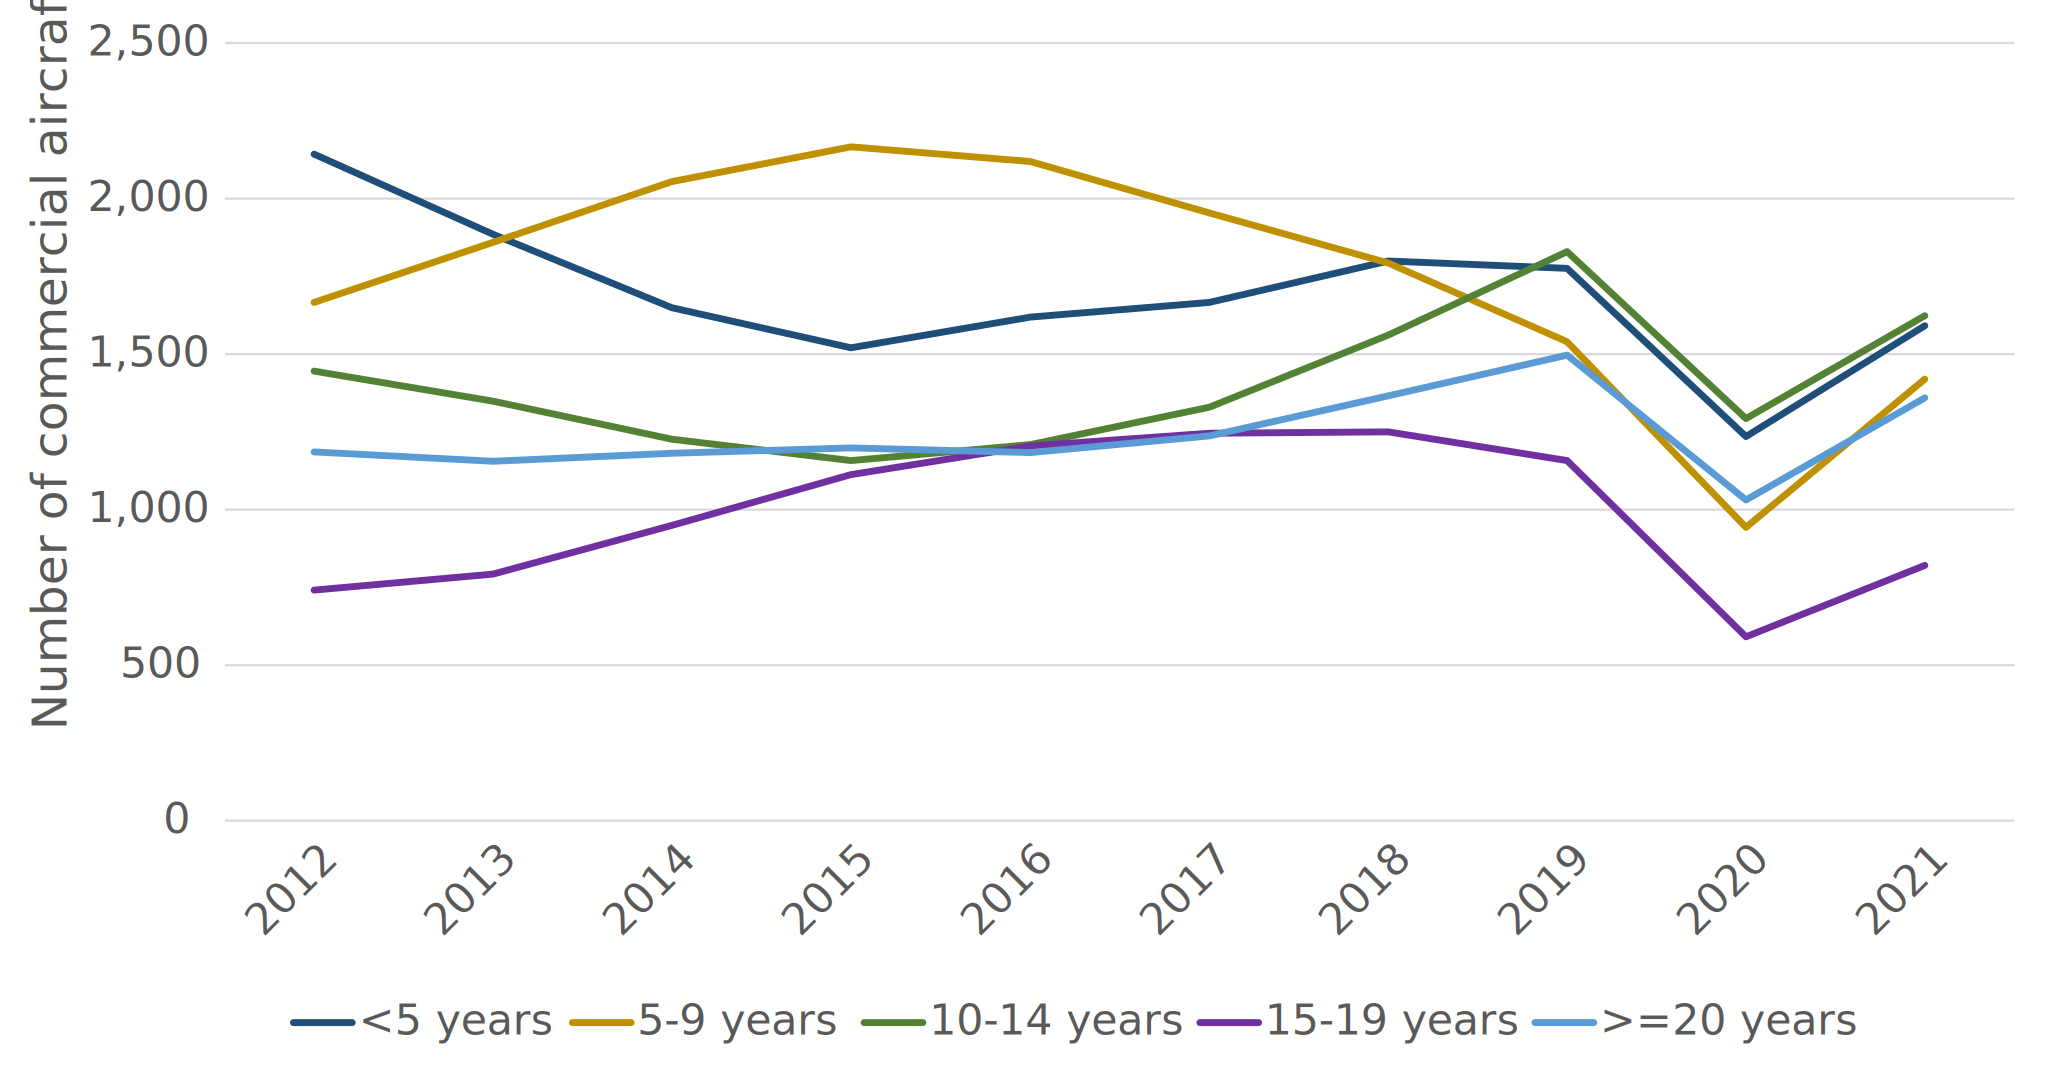
\includegraphics{chapters/../figures/aircraft-fleet-by-age.svg}

}

\caption{\label{fig-com-aircraft-fleet}Average aircraft age per flight
(EU27+EFTA+UK)\protect\hyperlink{ref-eurostataircraftfleet}{{[}50{]}}}

\end{figure}

EUROSTAT publishes annual statistics on commercial aircraft fleet by age
of aircraft and country of operator/country of registration.

\hypertarget{when-to-use-the-inputs-1}{%
\section{When to use the inputs?}\label{when-to-use-the-inputs-1}}

Depending on the market, an aircraft can remain in service for about 30
years. While an aircraft follows a specific maintenance cycle, its
performance can degrade over time due to engine and aerodynamic
deterioration, leading to additional CO\textsubscript{2} emissions.
Fleet renewal helps reduce aviation's environmental impact as newer
aircraft tend to be more fuel efficient and quieter, therefore the
average age of the European fleet is a good indicator of its
environmental performance.

\hypertarget{related-inputs-17}{%
\section{Related inputs}\label{related-inputs-17}}

Chapter~\ref{sec-number-of-ifr-flights}
\protect\hyperlink{sec-number-of-ifr-flights}{Number of IFR flights}

Chapter~\ref{sec-fleet-size} \protect\hyperlink{sec-fleet-size}{Fleet
size}

\hypertarget{references-23}{%
\section{References}\label{references-23}}

\hypertarget{sec-fleet-size}{%
\chapter{Fleet size}\label{sec-fleet-size}}

This input presents the number of aircraft, per type, operating in
Europe.

Table~\ref{tbl-fleet-size} shows the top 30 civil aircraft operating in
2022 in the airspace controlled by the EUROCONTROL Network Manager, by
aircraft type and number of aircraft.

\hypertarget{tbl-fleet-size}{}
\setlength{\LTpost}{0mm}
\begin{longtable}{lrrcccc}
\caption{\label{tbl-fleet-size}Top 30 civil aircraft operating in NM area }\tabularnewline

\toprule
Aircraft type & Number of aircraft & Number of flights & Proportion of aircraft & Cumulative & Proportion of flights & Cumulative \\ 
\midrule
B738 & $1,705$ & $1,722,929$ & $7.43\%$ & $7.43\%$ & $18.96\%$ & $18.96\%$ \\ 
A320 & $1,569$ & $1,421,804$ & $6.84\%$ & $14.27\%$ & $15.64\%$ & $34.60\%$ \\ 
B77W & $712$ & $164,394$ & $3.10\%$ & $17.37\%$ & $1.81\%$ & $36.41\%$ \\ 
GLF5 & $627$ & $15,601$ & $2.73\%$ & $20.10\%$ & $0.17\%$ & $36.58\%$ \\ 
GLEX & $565$ & $30,789$ & $2.46\%$ & $22.56\%$ & $0.34\%$ & $36.92\%$ \\ 
A20N & $557$ & $461,640$ & $2.43\%$ & $24.99\%$ & $5.08\%$ & $42.00\%$ \\ 
B789 & $508$ & $136,468$ & $2.21\%$ & $27.20\%$ & $1.50\%$ & $43.50\%$ \\ 
A21N & $499$ & $300,283$ & $2.17\%$ & $29.38\%$ & $3.30\%$ & $46.80\%$ \\ 
A319 & $478$ & $515,513$ & $2.08\%$ & $31.46\%$ & $5.67\%$ & $52.47\%$ \\ 
A321 & $473$ & $372,532$ & $2.06\%$ & $33.52\%$ & $4.10\%$ & $56.57\%$ \\ 
GLF4 & $454$ & $9,475$ & $1.98\%$ & $35.50\%$ & $0.10\%$ & $56.68\%$ \\ 
CL60 & $443$ & $24,016$ & $1.93\%$ & $37.43\%$ & $0.26\%$ & $56.94\%$ \\ 
DA42 & $436$ & $53,303$ & $1.90\%$ & $39.33\%$ & $0.59\%$ & $57.53\%$ \\ 
GLF6 & $429$ & $13,921$ & $1.87\%$ & $41.20\%$ & $0.15\%$ & $57.68\%$ \\ 
A333 & $418$ & $129,940$ & $1.82\%$ & $43.02\%$ & $1.43\%$ & $59.11\%$ \\ 
B763 & $384$ & $65,906$ & $1.67\%$ & $44.70\%$ & $0.73\%$ & $59.84\%$ \\ 
A359 & $368$ & $78,582$ & $1.60\%$ & $46.30\%$ & $0.86\%$ & $60.70\%$ \\ 
B38M & $365$ & $271,476$ & $1.59\%$ & $47.89\%$ & $2.99\%$ & $63.69\%$ \\ 
PC12 & $358$ & $55,886$ & $1.56\%$ & $49.45\%$ & $0.61\%$ & $64.30\%$ \\ 
A332 & $352$ & $86,506$ & $1.53\%$ & $50.98\%$ & $0.95\%$ & $65.25\%$ \\ 
F900 & $295$ & $10,078$ & $1.29\%$ & $52.27\%$ & $0.11\%$ & $65.37\%$ \\ 
B788 & $294$ & $80,970$ & $1.28\%$ & $53.55\%$ & $0.89\%$ & $66.26\%$ \\ 
F2TH & $284$ & $27,439$ & $1.24\%$ & $54.79\%$ & $0.30\%$ & $66.56\%$ \\ 
B77L & $258$ & $69,049$ & $1.12\%$ & $55.91\%$ & $0.76\%$ & $67.32\%$ \\ 
B744 & $254$ & $39,504$ & $1.11\%$ & $57.02\%$ & $0.43\%$ & $67.75\%$ \\ 
FA7X & $253$ & $13,650$ & $1.10\%$ & $58.12\%$ & $0.15\%$ & $67.90\%$ \\ 
B772 & $240$ & $66,430$ & $1.05\%$ & $59.17\%$ & $0.73\%$ & $68.63\%$ \\ 
PA34 & $239$ & $11,781$ & $1.04\%$ & $60.21\%$ & $0.13\%$ & $68.76\%$ \\ 
GL5T & $213$ & $10,043$ & $0.93\%$ & $61.14\%$ & $0.11\%$ & $68.87\%$ \\ 
BE20 & $206$ & $47,688$ & $0.90\%$ & $62.04\%$ & $0.52\%$ & $69.40\%$ \\ 
Other types & $8,712$ & $2,781,391$ & $37.96\%$ & $100.00\%$ & $30.60\%$ & $100.00\%$ \\ 
Total & $22,948$ & $9,088,987$ & $100.00\%$ & NA & $100.00\%$ & NA \\ 
\bottomrule
\end{longtable}
\begin{minipage}{\linewidth}
\emph{Source: EUROCONTROL Network Manager flight plans, 2022}\\
\end{minipage}

The 22,948 civil aircraft in Table~\ref{tbl-fleet-size} include 500
unique aircraft types. The top 30 aircraft types listed above represent
approximately 62\% of the total fleet, while 69\% of flights are
operated by the 300 most used aircraft types.

Table~\ref{tbl-military-aircraft} shows the number of military aircraft
by category in 2023 vs 2019 in Europe, USA, and Commonwealth of
Independent States (CIS) countries (Armenia, Azerbaijan, Belarus,
Kazakhstan, Kyrgyzstan, Moldova, Russia, Tajikistan and
Uzbekistan).\protect\hyperlink{ref-flightglobal2023}{{[}51{]}}

\hypertarget{tbl-military-aircraft}{}
\setlength{\LTpost}{0mm}
\begin{longtable}{lrrrrrr}
\caption{\label{tbl-military-aircraft}Military aircraft in 2023 vs 2019 }\tabularnewline

\toprule
Aircraft type & Europe 2019 & Europe 2023 & USA 2019 & USA 2023 & CIS 2019 & CIS 2023 \\ 
\midrule
Combat aircraft  & $2,066$ & $2,008$ & $2,879$ & $2,820$ & $1,936$ & $1,864$ \\ 
Special Mission\textsuperscript{1} & $245$ & $245$ & $780$ & $758$ & $125$ & $147$ \\ 
Tanker & $56$ & $49$ & $592$ & $638$ & $19$ & $19$ \\ 
Transport & $648$ & $588$ & $979$ & $990$ & $443$ & $484$ \\ 
Combat helicopter & $3,359$ & $3,328$ & $5,555$ & $5,704$ & $1,807$ & $1,915$ \\ 
Training aircraft/helicopters & $2,201$ & $1,912$ & $2,996$ & $2,766$ & $574$ & $624$ \\ 
Total military fleet & $8,575$ & $8,130$ & $13,781$ & $13,676$ & $4,904$ & $5,053$ \\ 
\% Difference 2023 vs 2019 & NA & $-5.19\%$ & NA & $-0.76\%$ & NA & $3.04\%$ \\ 
\bottomrule
\end{longtable}
\begin{minipage}{\linewidth}
\textsuperscript{1}Special Mission Aircraft are those platforms specifically developed to undertake an over-battlefield role by utilization of advanced onboard equipment or specialized trait\\
\emph{Source: \href{https://www.flightglobal.com/reports/2023-world-air-forces-directory/151088.article}{FlightGlobal (2023) 2023 World Air Forces directory}}\\
\end{minipage}

Table~\ref{tbl-ifr-helicopter} shows the fleet size of IFR helicopters
in Europe for years 2011/2012.

\hypertarget{tbl-ifr-helicopter}{}
\setlength{\LTpost}{0mm}
\begin{longtable}{lr}
\caption{\label{tbl-ifr-helicopter}IFR helicopter fleet }\tabularnewline

\toprule
Region & Units \\ 
\midrule
Europe and Eastern Europe & 2,208 \\ 
CIS countries & 1,312 \\ 
Total & 3,520 \\ 
\bottomrule
\end{longtable}
\begin{minipage}{\linewidth}
\emph{Source:  FlightGlobal HELICAS 2011/2012 data analysed by the \href{https://ext.eurocontrol.int/ground_navigation_infrastructure/homepage/welcome}{European Helicopter Association}}\\
\end{minipage}

Table~\ref{tbl-airframes} estimates the number of airframes operating
under Visual Flight Rules (VFR) in ECAC region.

\hypertarget{tbl-airframes}{}
\setlength{\LTpost}{0mm}
\begin{longtable}{lr}
\caption{\label{tbl-airframes}Number of VFR airframes in ECAC }\tabularnewline

\toprule
Aircraft & Units \\ 
\midrule
Aeroplanes & 20,329 \\ 
Helicopters & 3,532 \\ 
Gliders & 18,555 \\ 
Balloons & 6,623 \\ 
Total & 49,039 \\ 
\bottomrule
\end{longtable}
\begin{minipage}{\linewidth}
\emph{Source: \href{https://www.icao.int/secretariat/legal/Pages/Intl_registry.aspx}{International Registry of Civil Aircraft (IRCA), 2014} and \href{https://www.aopa.org/}{Aircraft Owners and Pilot Association (AOPA) (2015)}}\\
\end{minipage}

\hypertarget{other-possible-sources---forward-looking}{%
\section{Other possible sources -
forward-looking}\label{other-possible-sources---forward-looking}}

The \textbf{Airbus Global Market Forecast for 2022-2041} presents a
forward-looking view of the evolution of the air transport sector,
accounting for factors such as demographic and economic growth, tourism
trends, oil prices, the development of new and existing routes, and
ultimately highlighting demand for aircraft covering the spectrum of
sizes from 100 seats to the very largest aircraft of over 500 seats.

\begin{figure}

{\centering 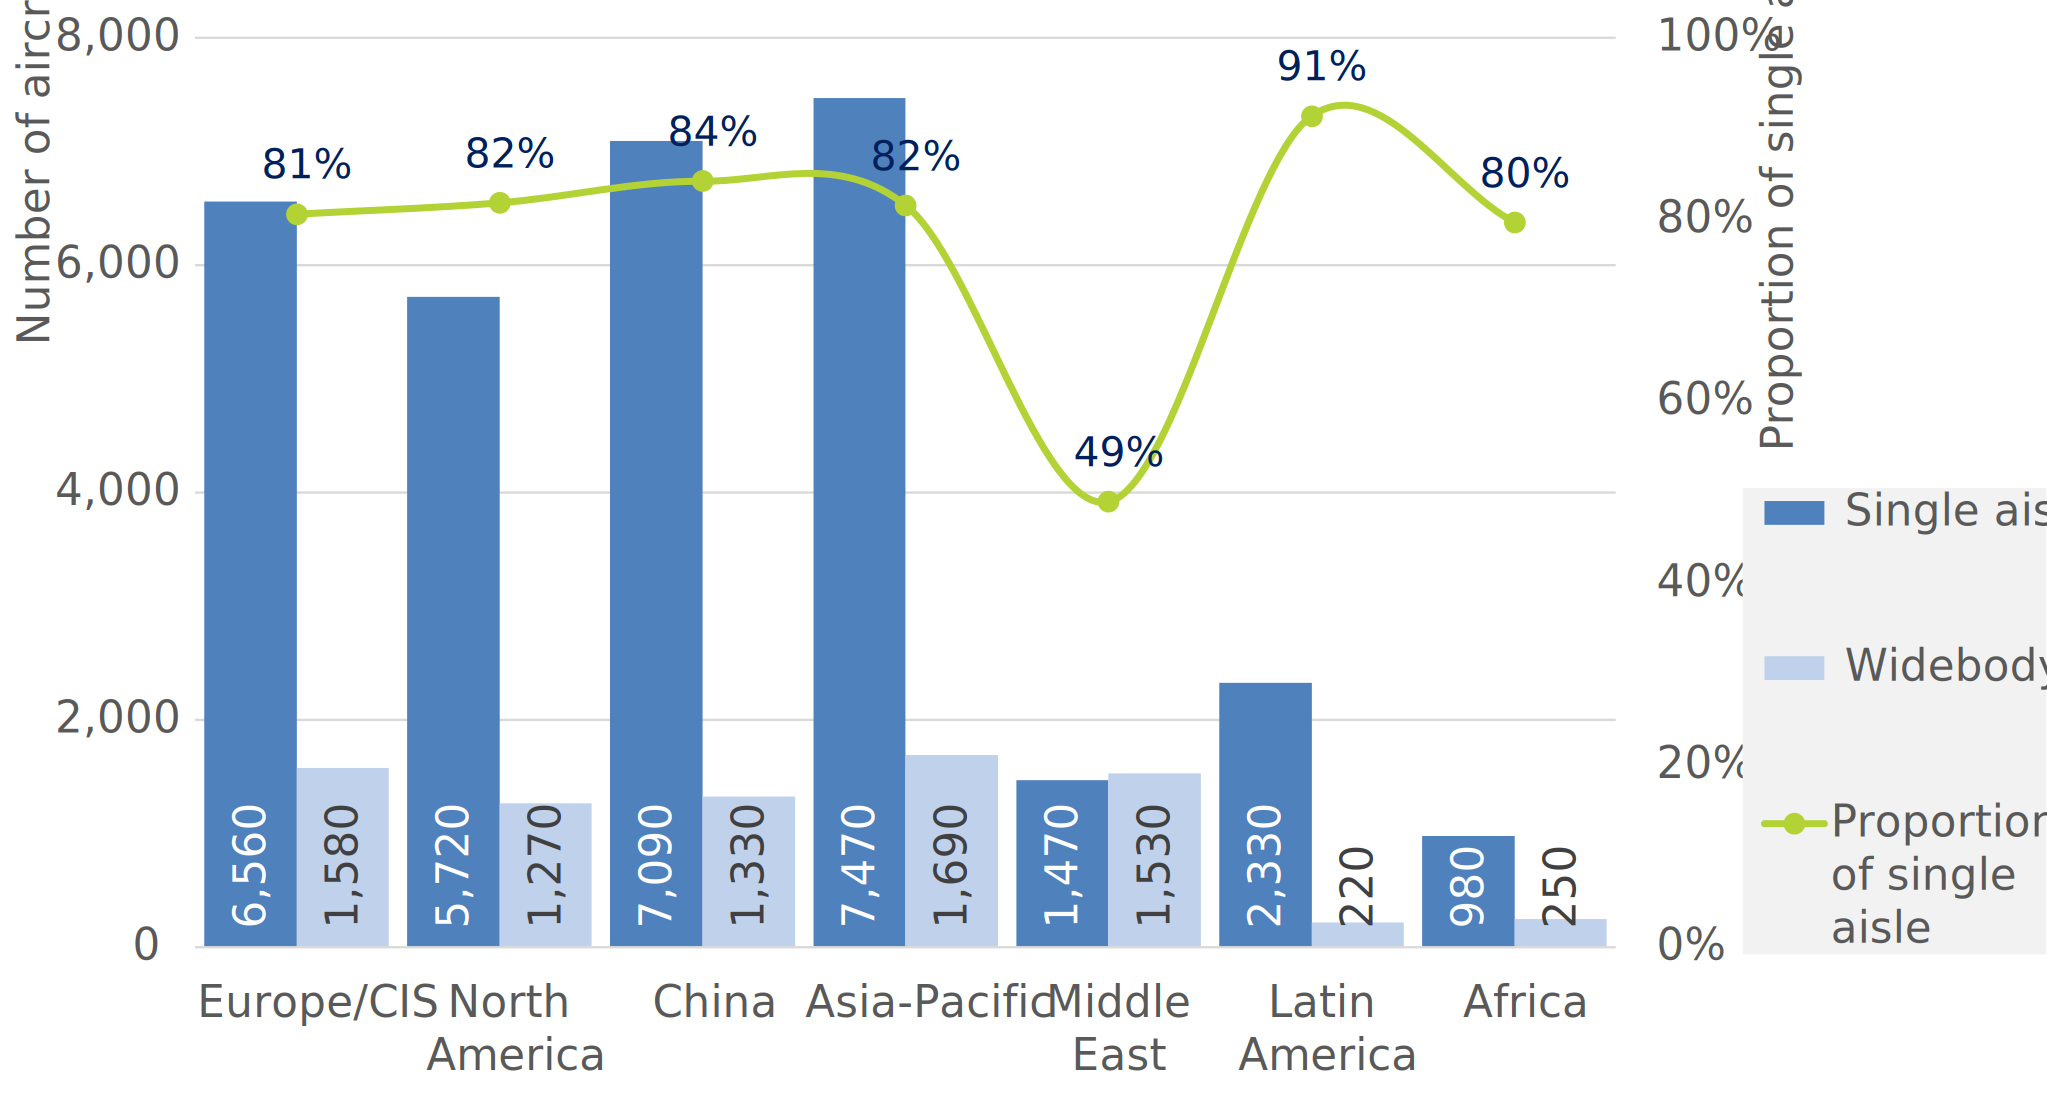
\includegraphics{chapters/../figures/airbus_demand.svg}

}

\caption{\label{fig-airbus-demand}Airbus commercial aircraft demand
2022-2041 \protect\hyperlink{ref-airbusGMF2022}{{[}52{]}}}

\end{figure}

As shown in Figure~\ref{fig-airbus-demand}, for the years 2022-2041,
Airbus forecasts a demand for 39,490 new or replacement commercial
aircraft worldwide, of which 8,140 units (21\%) are for Europe/CIS
regions. Asia-Pacific, China and the US are driving the growth, while
single-aisle aircraft dominate the demand (\textgreater80\%).

Figure~\ref{fig-boeing-demand} shows the Boeing forecast demand for new
aircraft by category and world regions with a focus on single-aisle
aircraft which leads the market growth.

\begin{figure}

{\centering 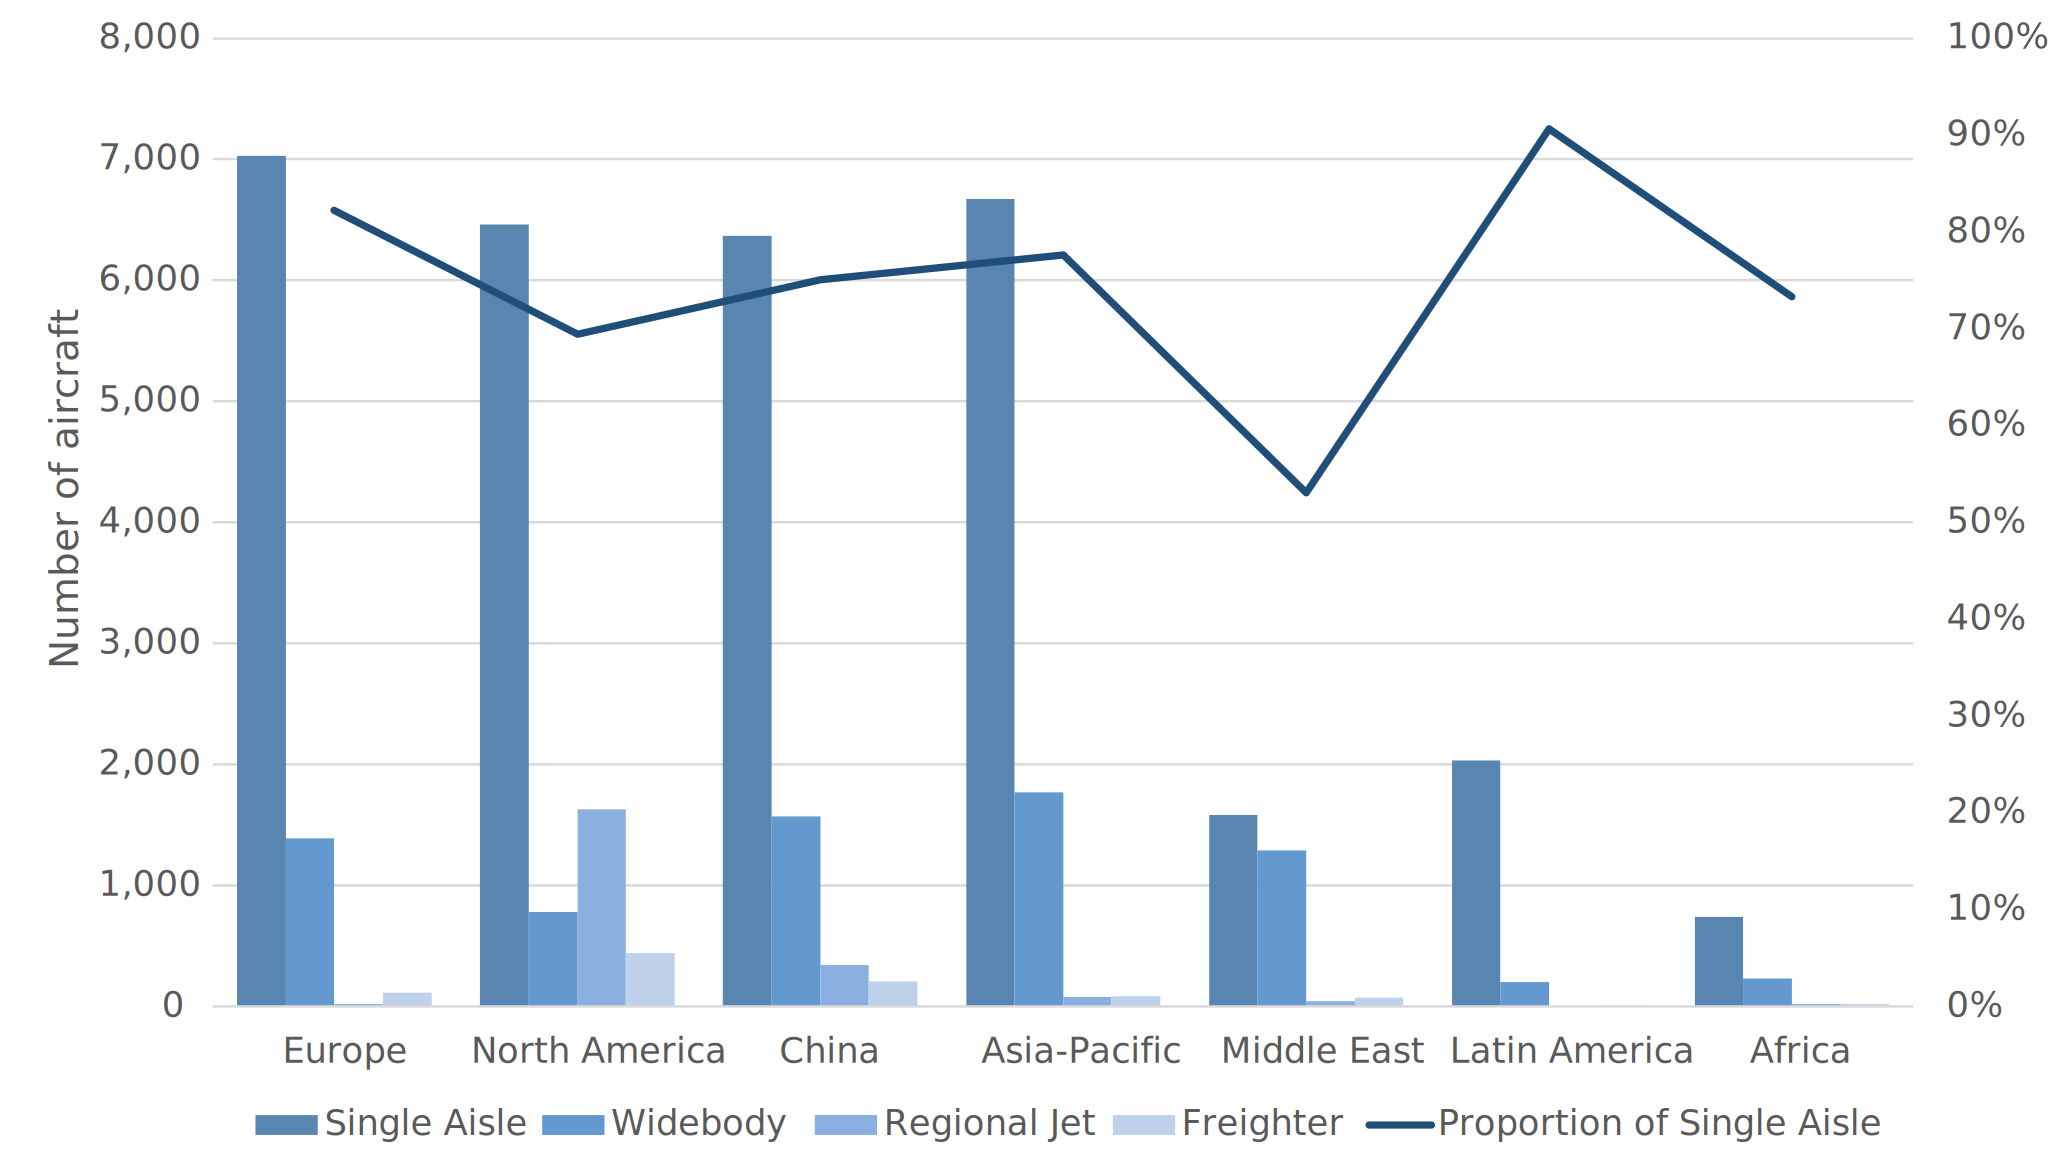
\includegraphics{chapters/../figures/boeing_demand.svg}

}

\caption{\label{fig-boeing-demand}Boeing commercial aircraft demand
2022-2041 \protect\hyperlink{ref-boeingcmf2022}{{[}53{]}}}

\end{figure}

For the same period (2022-2041), \textbf{Boeing forecasts} a global
demand for 40,170 new or replacement commercial aircraft of which 8,550
units (21\%) are for Europe. Europe, Asia-Pacific, US and China are the
drivers for growth owing to the demand for single-aisle aircraft which
represents between 69\% (in US) and 82\% (in Europe) of the total fleet
forecast.

\hypertarget{related-inputs-18}{%
\section{Related inputs}\label{related-inputs-18}}

Chapter~\ref{sec-number-of-ifr-flights}
\protect\hyperlink{sec-number-of-ifr-flights}{Number of IFR flights}

Chapter~\ref{sec-ifr-flight-information-per-market-segment}
\protect\hyperlink{sec-ifr-flight-information-per-market-segment}{IFR
flight information per market segment}

Chapter~\ref{sec-fleet-age} \protect\hyperlink{sec-fleet-age}{Fleet age}

\hypertarget{references-24}{%
\section{References}\label{references-24}}

\hypertarget{sec-fleet-cns-capability}{%
\chapter{Fleet CNS capability}\label{sec-fleet-cns-capability}}

\hypertarget{eurocontrol-recommended-values-23}{%
\section{EUROCONTROL recommended
values}\label{eurocontrol-recommended-values-23}}

The subsections below provide statistics on flights and aircraft with
certain Communication, Navigation and Surveillance (CNS) equipment and
capabilities.

\hypertarget{navigation-nav-flight-capabilities}{%
\subsection{Navigation (NAV) flight
capabilities}\label{navigation-nav-flight-capabilities}}

The values presented in the tables hereafter are weighted by flight and
represent the values for
2019.\protect\hyperlink{ref-cns:dashboard}{{[}54{]}}

\hypertarget{tbl-nav-flight}{}
\setlength{\LTpost}{0mm}
\begin{longtable}{lrc}
\caption{\label{tbl-nav-flight}NAV flight capabilities as a \% of total flights }\tabularnewline

\toprule
Capability & Number of flights\textsuperscript{1} & As a \% of all flights \\ 
\midrule
A – GBAS landing system & $1,066,532$ & $4.8\%$ \\ 
B – LPV (APV with SBAS) & $1,154,182$ & $5.2\%$ \\ 
D – RNAV 1 & $20,771,164$ & $93.5\%$ \\ 
O –- Basic RNP 1 & $15,788,068$ & $71.1\%$ \\ 
S – RNP APCH & $19,241,254$ & $86.6\%$ \\ 
\bottomrule
\end{longtable}
\begin{minipage}{\linewidth}
\textsuperscript{1}The number of flights is number of arrivals or departures, or arrivals and departures in line with the selection criteria in the CNS dashboard\\
\emph{Source: \href{https://www.eurocontrol.int/dashboard/communication-navigation-and-surveillance-dashboard}{EUROCONTROL Communication, Navigation \& Surveillance (CNS) Dashboard}}\\
\end{minipage}

\hypertarget{tbl-nav-flight_top10}{}
\setlength{\LTpost}{0mm}
\begin{longtable}{lccccc}
\caption{\label{tbl-nav-flight_top10}NAV flight capabilities as a \% at the top 10 European Airports }\tabularnewline

\toprule
Airport & A - GBAS landing system\textsuperscript{1} & B - LPV (APV with SBAS) & D - RNAV 1 & O - Basic RNP 1 & S - RNP APCH \\ 
\midrule
Barcelona & $2.6\%$ & $2.4\%$ & $97.4\%$ & $89.5\%$ & $94.6\%$ \\ 
Frankfurt Main & $6.7\%$ & $2.0\%$ & $97.7\%$ & $89.1\%$ & $94.0\%$ \\ 
Istanbul/New airport & $0.8\%$ & $0.3\%$ & $97.1\%$ & $91.3\%$ & $93.1\%$ \\ 
London/Gatwick & $4.2\%$ & $0.9\%$ & $97.9\%$ & $88.2\%$ & $95.4\%$ \\ 
London/Heathrow & $7.5\%$ & $1.6\%$ & $98.0\%$ & $88.1\%$ & $96.7\%$ \\ 
Madrid Barajas & $2.1\%$ & $10.0\%$ & $97.0\%$ & $72.8\%$ & $89.6\%$ \\ 
Munich 2 & $2.7\%$ & $3.0\%$ & $97.4\%$ & $90.5\%$ & $88.7\%$ \\ 
Paris Ch de Gaulle & $2.6\%$ & $1.1\%$ & $97.9\%$ & $79.4\%$ & $92.7\%$ \\ 
Rome Fiumicino & $2.2\%$ & $0.5\%$ & $97.9\%$ & $90.6\%$ & $93.9\%$ \\ 
Schiphol Amsterdam & $1.9\%$ & $1.5\%$ & $97.9\%$ & $87.5\%$ & $95.7\%$ \\ 
\bottomrule
\end{longtable}
\begin{minipage}{\linewidth}
\textsuperscript{1}The values for GBAS are corrected values. They exclude DHC8 equipment only compatible with a GBAS precursor system\\
\emph{Source: \href{https://www.eurocontrol.int/dashboard/communication-navigation-and-surveillance-dashboard}{EUROCONTROL Communication, Navigation \& Surveillance (CNS) Dashboard}}\\
\end{minipage}

\hypertarget{tbl-nav-flight_month}{}
\setlength{\LTpost}{0mm}
\begin{longtable}{lccccc}
\caption{\label{tbl-nav-flight_month}NAV aircraft capability over a one-month period, July 2019 }\tabularnewline

\toprule
Airport & A - GBAS landing system & B - LPV (APV with SBAS) & D - RNAV 1 & O - Basic RNP 1 & S - RNP APCH \\ 
\midrule
Barcelona & $6.0\%$ & $7.2\%$ & $98.8\%$ & $85.0\%$ & $94.8\%$ \\ 
Frankfurt Main & $8.1\%$ & $6.7\%$ & $98.8\%$ & $82.4\%$ & $95.1\%$ \\ 
Istanbul/New airport & $4.7\%$ & $1.7\%$ & $98.2\%$ & $87.8\%$ & $90.2\%$ \\ 
London/Gatwick & $9.7\%$ & $2.9\%$ & $99.5\%$ & $87.0\%$ & $96.5\%$ \\ 
London/Heathrow & $10.7\%$ & $2.2\%$ & $99.9\%$ & $87.9\%$ & $97.9\%$ \\ 
Madrid Barajas & $8.1\%$ & $8.2\%$ & $98.2\%$ & $81.4\%$ & $93.1\%$ \\ 
Munich 2 & $6.1\%$ & $7.3\%$ & $98.3\%$ & $83.2\%$ & $94.6\%$ \\ 
Paris Ch de Gaulle & $6.5\%$ & $2.6\%$ & $99.7\%$ & $82.1\%$ & $93.9\%$ \\ 
Rome Fiumicino & $6.2\%$ & $1.4\%$ & $99.5\%$ & $86.6\%$ & $94.0\%$ \\ 
Schiphol Amsterdam & $5.6\%$ & $6.0\%$ & $98.9\%$ & $80.5\%$ & $95.9\%$ \\ 
\bottomrule
\end{longtable}
\begin{minipage}{\linewidth}
\emph{Source: \href{https://www.eurocontrol.int/dashboard/communication-navigation-and-surveillance-dashboard}{EUROCONTROL Communication, Navigation \& Surveillance (CNS) Dashboard}}\\
\end{minipage}

\hypertarget{tbl-nav-flight_aircraft}{}
\setlength{\LTpost}{0mm}
\begin{longtable}{lccccc}
\caption{\label{tbl-nav-flight_aircraft}NAV flight capability by main aircraft model }\tabularnewline

\toprule
Aircraft & A - GBAS landing system & B - LPV (APV with SBAS)\textsuperscript{1} & D - RNAV 1 & O - Basic RNP 1 & S - RNP APCH \\ 
\midrule
B737 & $7.1\%$ & $0.3\%$ & $97.4\%$ & $80.9\%$ & $90.2\%$ \\ 
A320 & $1.0\%$ & $0.1\%$ & $97.8\%$ & $80.5\%$ & $92.9\%$ \\ 
A319 & $1.0\%$ & $0.0\%$ & $97.9\%$ & $78.4\%$ & $96.1\%$ \\ 
A321 & $4.4\%$ & $0.0\%$ & $98.0\%$ & $85.9\%$ & $96.4\%$ \\ 
DHC8 & $18.6\%$\textsuperscript{2} & $6.4\%$ & $96.2\%$ & $17.1\%$ & $88.9\%$ \\ 
ATR72 & $2.0\%$ & $5.7\%$ & $76.9\%$ & $16.2\%$ & $60.4\%$ \\ 
B777 & $0.1\%$ & $0.0\%$ & $98.0\%$ & $97.6\%$ & $96.4\%$ \\ 
A330 & $0.1\%$ & $0.6\%$ & $97.6\%$ & $88.8\%$ & $92.0\%$ \\ 
E190 & $1.1\%$ & $0.0\%$ & $98.0\%$ & $64.7\%$ & $96.4\%$ \\ 
A320 NEO & $0.4\%$ & $0.0\%$ & $98.0\%$ & $91.9\%$ & $97.7\%$ \\ 
B787 & $44.2\%$ & $0.0\%$ & $97.9\%$ & $96.1\%$ & $93.3\%$ \\ 
CL900RJ & $0.0\%$ & $0.0\%$ & $98.0\%$ & $88.5\%$ & $88.1\%$ \\ 
E195 & $0.0\%$ & $0.0\%$ & $96.2\%$ & $44.5\%$ & $86.3\%$ \\ 
B767 & $0.0\%$ & $0.0\%$ & $97.7\%$ & $81.1\%$ & $79.2\%$ \\ 
E175 & $0.0\%$ & $0.0\%$ & $97.6\%$ & $65.1\%$ & $97.5\%$ \\ 
\bottomrule
\end{longtable}
\begin{minipage}{\linewidth}
\textsuperscript{1}The values for A319, A320, A330 and B737 aircraft (0.00\%) are corrected values, as no such capability exist for these aircraft\\
\textsuperscript{2}This percentage represent the equipage rate of a GBAS precursor system called S-CATI\\
\emph{Source: \href{https://www.eurocontrol.int/dashboard/communication-navigation-and-surveillance-dashboard}{EUROCONTROL Communication, Navigation \& Surveillance (CNS) Dashboard}}\\
\end{minipage}

\hypertarget{communication-com-flight-capabilities}{%
\subsection{Communication (COM) flight
capabilities}\label{communication-com-flight-capabilities}}

The values presented in the tables hereafter are weighted by flight and
represent values for year
2019.\protect\hyperlink{ref-cns:dashboard}{{[}54{]}}

\hypertarget{tbl-com-flight}{}
\setlength{\LTpost}{0mm}
\begin{longtable}{lrc}
\caption{\label{tbl-com-flight}COM flight capabilities as a \% of total flights }\tabularnewline

\toprule
Capability & Number of flights & As a \% of all flights \\ 
\midrule
\multicolumn{3}{l}{Datalink} \\ 
\midrule
E2 - D-FIS ACARS & $9,160,750$ & $41.2\%$ \\ 
E3 - PDC ACARS & $10,252,210$ & $46.2\%$ \\ 
J1 - CPDLC ATN VDL Mode 2 & $7,065,296$ & $31.8\%$ \\ 
J4 - CPDLC FANS 1/A VDL Mode 2 & $2,070,030$ & $9.3\%$ \\ 
J5 - CPDLC FANS 1/A SATCOM (INMARSAT) & $2,654,930$ & $1.7\%$ \\ 
J7 - CPDLC FANS 1/A SATCOM (iridium) & $385,784$ & $1.7\%$ \\ 
\midrule
\multicolumn{3}{l}{Voice} \\ 
\midrule
H - HF RTF & $10,825,396$ & $48.7\%$ \\ 
M1 - ATC RTF SATCOM (INMARSAT) & $2,705,550$ & $12.2\%$ \\ 
M2 - ATC RTF (MTSAT) & $276,730$ & $1.3\%$ \\ 
M3 - ATC RTF (iridium) & $613,286$ & $2.8\%$ \\ 
U - UHF RTF & $585,788$ & $2.6\%$ \\ 
V - VHF RTF & $2,945,674$ & $13.3\%$ \\ 
Y - VHF with 8.33 kHz channel spacing capability & $22,018,258$ & $99.1\%$ \\ 
\bottomrule
\end{longtable}
\begin{minipage}{\linewidth}
\emph{Source: \href{https://www.eurocontrol.int/dashboard/communication-navigation-and-surveillance-dashboard}{EUROCONTROL Communication, Navigation \& Surveillance (CNS) Dashboard}}\\
\end{minipage}

\hypertarget{tbl-com-flight_top10}{}
\setlength{\LTpost}{0mm}
\begin{longtable}{lcccccc}
\caption{\label{tbl-com-flight_top10}COM datalink flight capabilities as a \% at the top 10 European airports }\tabularnewline

\toprule
Airport & E2 - D-FIS ACARS & E3 - PDC ACARS & J1 - CPDLC ATN VDL Mode 2 & J4 - CPDLC FANS 1/A VDL Mode 2 & J5 - CPDLC FANS 1/A SATCOM (INMARSAT) & J7 - CPDLC FANS 1/A SATCOM (IRIDIUM) \\ 
\midrule
Barcelona & $26.0\%$ & $31.5\%$ & $21.9\%$ & $5.8\%$ & $6.6\%$ & $0.8\%$ \\ 
Frankfurt Main & $78.8\%$ & $73.3\%$ & $48.7\%$ & $15.4\%$ & $18.7\%$ & $3.8\%$ \\ 
Istanbul/New airport & $83.4\%$ & $83.5\%$ & $66.7\%$ & $22.8\%$ & $23.2\%$ & $0.2\%$ \\ 
London/Gatwick & $64.5\%$ & $75.4\%$ & $69.0\%$ & $6.2\%$ & $10.9\%$ & $1.6\%$ \\ 
London/Heathrow & $31.9\%$ & $88.5\%$ & $36.1\%$ & $18.7\%$ & $36.8\%$ & $2.3\%$ \\ 
Madrid Barajas & $20.5\%$ & $28.0\%$ & $23.4\%$ & $11.4\%$ & $16.2\%$ & $0.7\%$ \\ 
Munich 2 & $80.7\%$ & $67.8\%$ & $41.1\%$ & $8.2\%$ & $8.9\%$ & $0.9\%$ \\ 
Paris Ch de Gaulle & $72.9\%$ & $76.5\%$ & $54.3\%$ & $11.5\%$ & $21.7\%$ & $2.7\%$ \\ 
Rome Fiumicino & $23.3\%$ & $28.3\%$ & $29.6\%$ & $7.8\%$ & $11.3\%$ & $1.1\%$ \\ 
Schiphol Amsterdam & $79.9\%$ & $82.8\%$ & $20.8\%$ & $5.7\%$ & $15.7\%$ & $2.3\%$ \\ 
\bottomrule
\end{longtable}
\begin{minipage}{\linewidth}
\emph{Source: \href{https://www.eurocontrol.int/dashboard/communication-navigation-and-surveillance-dashboard}{EUROCONTROL Communication, Navigation \& Surveillance (CNS) Dashboard}}\\
\end{minipage}

\hypertarget{tbl-com-voice-top10}{}
\setlength{\LTpost}{0mm}
\begin{longtable}{lccccccccr}
\caption{\label{tbl-com-voice-top10}COM voice flight capabilities as a \% at the top 10 European airports }\tabularnewline

\toprule
Airport & H – HF RTF & M1 – ATC RTF SATCOM (INMARSAT) & M2 – ATC RTF (MTSAT) & M3 – ATC RTF (IRIDIUM) & U – UHF RTF & V – VHF RTF & Y – VHF with 8.33 kHz channel spacing & ...9 & ...10 \\ 
\midrule
Barcelona & $65.8\%$ & $9.1\%$ & $0.0\%$ & $1.7\%$ & $0.8\%$ & $41.8\%$ & $99.9\%$ & NA & NA \\ 
Frankfurt Main & $32.0\%$ & $18.4\%$ & $0.4\%$ & $3.5\%$ & $0.8\%$ & $7.2\%$ & $99.9\%$ & NA & NA \\ 
Istanbul/New airport & $95.1\%$ & $19.8\%$ & $0.0\%$ & $2.1\%$ & $1.0\%$ & $9.6\%$ & $100.0\%$ & NA & NA \\ 
London/Gatwick & $68.9\%$ & $9.8\%$ & $2.9\%$ & $0.8\%$ & $0.7\%$ & $9.0\%$ & $100.0\%$ & NA & NA \\ 
London/Heathrow & $58.3\%$ & $36.8\%$ & $14.1\%$ & $2.6\%$ & $1.2\%$ & $5.7\%$ & $100.0\%$ & NA & NA \\ 
Madrid Barajas & $63.2\%$ & $32.1\%$ & $0.4\%$ & $1.1\%$ & $0.6\%$ & $5.0\%$ & $99.9\%$ & NA & NA \\ 
Munich 2 & $24.6\%$ & $9.4\%$ & $0.2\%$ & $1.4\%$ & $1.1\%$ & $6.1\%$ & $99.9\%$ & NA & NA \\ 
Paris  Ch de Gaulle & $48.7\%$ & $21.9\%$ & $7.7\%$ & $3.5\%$ & $1.0\%$ & $7.7\%$ & $99.6\%$ & NA & NA \\ 
Rome Fiumicino & $39.1\%$ & $12.1\%$ & $0.2\%$ & $1.3\%$ & $1.1\%$ & $13.3\%$ & $100.0\%$ & NA & NA \\ 
Schiphol Amsterdam & $40.8\%$ & $8.0\%$ & $0.0\%$ & $2.7\%$ & $0.4\%$ & $6.5\%$ & $99.8\%$ & NA & NA \\ 
NA & NA & NA & NA & NA & NA & NA & NA & NA & NA \\ 
NA & NA & NA & NA & NA & NA & NA & NA & NA & NA \\ 
NA & NA & NA & NA & NA & NA & NA & NA & NA & NA \\ 
NA & NA & NA & NA & NA & NA & NA & NA & NA & NA \\ 
NA & NA & NA & NA & NA & NA & NA & NA & NA & NA \\ 
NA & NA & NA & NA & NA & NA & NA & NA & NA & NA \\ 
NA & NA & NA & NA & NA & NA & NA & NA & NA & 12.5 \\ 
\bottomrule
\end{longtable}
\begin{minipage}{\linewidth}
\emph{Source: \href{https://www.eurocontrol.int/dashboard/communication-navigation-and-surveillance-dashboard}{EUROCONTROL Communication, Navigation \& Surveillance (CNS) Dashboard}}\\
\end{minipage}

\hypertarget{tbl-com-aircraft}{}
\setlength{\LTpost}{0mm}
\begin{longtable}{lcccccc}
\caption{\label{tbl-com-aircraft}COM datalink flight capabilities for main aircraft models }\tabularnewline

\toprule
Aircraft & E2 - D-FIS ACARS & E3 - PDC ACARS & J1 - CPDLC ATN VDL Mode 2 & J4 - CPDLC FANS 1/A VDL Mode 2 & J5 - CPDLC FANS 1/A SATCOM (INMARSAT) & J7 - CPDLC FANS 1/A SATCOM (IRIDIUM) \\ 
\midrule
B737 & $22.5\%$ & $28.8\%$ & $27.1\%$ & $1.0\%$ & $0.2\%$ & $0.2\%$ \\ 
A320 & $62.5\%$ & $62.0\%$ & $52.1\%$ & $3.5\%$ & $0.1\%$ & $0.0\%$ \\ 
A319 & $63.3\%$ & $75.7\%$ & $51.1\%$ & $0.6\%$ & $0.4\%$ & $0.0\%$ \\ 
A321 & $70.2\%$ & $70.5\%$ & $59.3\%$ & $5.0\%$ & $0.2\%$ & $0.4\%$ \\ 
DHC8 & $12.6\%$ & $6.3\%$ & $0.0\%$ & $0.0\%$ & $0.1\%$ & $31.5\%$ \\ 
ATR72 & $8.2\%$ & $11.4\%$ & $0.0\%$ & $0.0\%$ & $0.0\%$ & $0.0\%$ \\ 
B777 & $62.3\%$ & $93.3\%$ & $26.8\%$ & $49.2\%$ & $96.9\%$ & $8.1\%$ \\ 
A330 & $61.0\%$ & $82.3\%$ & $3.6\%$ & $56.1\%$ & $90.5\%$ & $4.7\%$ \\ 
E190 & $71.5\%$ & $67.4\%$ & $27.9\%$ & $0.0\%$ & $0.0\%$ & $0.0\%$ \\ 
A320 NEO & $32.7\%$ & $52.9\%$ & $61.2\%$ & $0.3\%$ & $0.0\%$ & $0.1\%$ \\ 
B787 & $62.1\%$ & $77.2\%$ & $67.5\%$ & $82.5\%$ & $98.9\%$ & $3.6\%$ \\ 
CL900RJ & $47.6\%$ & $0.2\%$ & $0.0\%$ & $0.0\%$ & $100.0\%$ & $65.9\%$ \\ 
E195 & $65.9\%$ & $57.8\%$ & $42.1\%$ & $0.4\%$ & $22.3\%$ & $100.0\%$ \\ 
B767 & $38.9\%$ & $66.5\%$ & $1.4\%$ & $28.1\%$ & $37.5\%$ & $36.9\%$ \\ 
E175 & $55.8\%$ & $54.3\%$ & $48.7\%$ & $0.4\%$ & $0.5\%$ & $16.4\%$ \\ 
\bottomrule
\end{longtable}
\begin{minipage}{\linewidth}
\emph{Source: \href{https://www.eurocontrol.int/dashboard/communication-navigation-and-surveillance-dashboard}{EUROCONTROL Communication, Navigation \& Surveillance (CNS) Dashboard}}\\
\end{minipage}

\hypertarget{tbl-com-voice-aircraft}{}
\setlength{\LTpost}{0mm}
\begin{longtable}{lccccccc}
\caption{\label{tbl-com-voice-aircraft}COM voice flight capabilities for main aircraft models }\tabularnewline

\toprule
Airport & H – HF RTF & M1 – ATC RTF SATCOM (INMARSAT) & M2 – ATC RTF (MTSAT) & M3 – ATC RTF (IRIDIUM) & U – UHF RTF & V – VHF RTF & Y – VHF with 8.33 kHz channel spacing \\ 
\midrule
B737 & $22.5\%$ & $28.8\%$ & $27.1\%$ & $1.0\%$ & $0.2\%$ & $0.2\%$ & $53.4\%$ \\ 
A320 & $62.5\%$ & $62.0\%$ & $52.1\%$ & $3.5\%$ & $0.1\%$ & $0.0\%$ & $63.9\%$ \\ 
A319 & $63.3\%$ & $75.7\%$ & $51.1\%$ & $0.6\%$ & $0.4\%$ & $0.0\%$ & $25.1\%$ \\ 
A321 & $70.2\%$ & $70.5\%$ & $59.3\%$ & $5.0\%$ & $0.2\%$ & $0.4\%$ & $51.8\%$ \\ 
DHC8 & $12.6\%$ & $6.3\%$ & $0.0\%$ & $0.0\%$ & $0.1\%$ & $31.5\%$ & $4.2\%$ \\ 
ATR72 & $8.2\%$ & $11.4\%$ & $0.0\%$ & $0.0\%$ & $0.0\%$ & $0.0\%$ & $11.5\%$ \\ 
B777 & $62.3\%$ & $93.3\%$ & $26.8\%$ & $49.2\%$ & $96.9\%$ & $8.1\%$ & $99.9\%$ \\ 
A330 & $61.0\%$ & $82.3\%$ & $3.6\%$ & $56.1\%$ & $90.5\%$ & $4.7\%$ & $99.9\%$ \\ 
E190 & $71.5\%$ & $67.4\%$ & $27.9\%$ & $0.0\%$ & $0.0\%$ & $0.0\%$ & $26.0\%$ \\ 
A320 NEO & $32.7\%$ & $52.9\%$ & $61.2\%$ & $0.3\%$ & $0.0\%$ & $0.1\%$ & $32.4\%$ \\ 
B787 & $62.1\%$ & $77.2\%$ & $67.5\%$ & $82.5\%$ & $98.9\%$ & $3.6\%$ & $99.8\%$ \\ 
CL900RJ & $47.6\%$ & $0.2\%$ & $0.0\%$ & $0.0\%$ & $100.0\%$ & $65.9\%$ & $0.4\%$ \\ 
E195 & $65.9\%$ & $57.8\%$ & $42.1\%$ & $0.4\%$ & $22.3\%$ & $100.0\%$ & $21.3\%$ \\ 
B767 & $38.9\%$ & $66.5\%$ & $1.4\%$ & $28.1\%$ & $37.5\%$ & $36.9\%$ & $97.8\%$ \\ 
E175 & $55.8\%$ & $54.3\%$ & $48.7\%$ & $0.4\%$ & $0.5\%$ & $16.4\%$ & $5.4\%$ \\ 
\bottomrule
\end{longtable}
\begin{minipage}{\linewidth}
\emph{Source: \href{https://www.eurocontrol.int/dashboard/communication-navigation-and-surveillance-dashboard}{EUROCONTROL Communication, Navigation \& Surveillance (CNS) Dashboard}}\\
\end{minipage}

\hypertarget{surveillance-sur-flight-capabilities}{%
\subsection{Surveillance (SUR) flight
capabilities}\label{surveillance-sur-flight-capabilities}}

The values presented in the tables hereafter are weighted by flight and
represent the values for
2022.\protect\hyperlink{ref-cns:dashboard}{{[}54{]}}

\hypertarget{tbl-sur-flight}{}
\setlength{\LTpost}{0mm}
\begin{longtable}{lrc}
\caption{\label{tbl-sur-flight}SUR flight capabilities as a \% of total flights }\tabularnewline

\toprule
Capability & Number of flights\textsuperscript{1} & As a \% of all flights \\ 
\midrule
\multicolumn{3}{l}{SSR Mode S} \\ 
\midrule
L – Mode S, including aircraft identification, pressure-altitude, extended squitter (ADS-B) and enhanced surveillance capability & $4,841,403$ & $52.3\%$ \\ 
H – Mode S, including aircraft identification, pressure-altitude and enhanced surveillance capability & $1,437,964$ & $15.5\%$ \\ 
E – Mode S, including aircraft identification, pressure-altitude and extended squitter (ADS-B) capability & $274,513$ & $3.0\%$ \\ 
S – Mode S, including both pressure-altitude and aircraft identification capability & $2,645,524$ & $28.6\%$ \\ 
P – Mode S, including pressure-altitude, but no aircraft identification capability & $2,729$ & $0.0\%$ \\ 
I – Mode S, including aircraft identification, but no pressure-altitude capability & $975$ & $0.0\%$ \\ 
X – Mode S with neither aircraft identification nor pressure-altitude capability & $3,512$ & $0.0\%$ \\ 
C – Mode A (4 digits - 4096 codes) and Mode C & $122,008$ & $1.3\%$ \\ 
A – Mode A (4 digits - 4096 codes) & $88,646$ & $1.0\%$ \\ 
\midrule
\multicolumn{3}{l}{ADS-B} \\ 
\midrule
B1 – ADS-B with dedicated 1090 MHz ADS-B “out” capability & $7,409,392$ & $80.1\%$ \\ 
B2 – ADB-B with dedicated 1090 MHz ADS-B “out” and “in” capability & $329,079$ & $3.6\%$ \\ 
U1 – ADS-B “out” capability using UAT & $44,076$ & $0.5\%$ \\ 
U2 – ADS-B “out” and “in” capability using UAT & $9,195$ & $0.1\%$ \\ 
V1 – ADS-B “out” capability using VDL Mode 4 & $64,899$ & $0.7\%$ \\ 
V2 – ADS-B “out” and “in” capability using VDL Mode 4 & $6,092$ & $0.1\%$ \\ 
\bottomrule
\end{longtable}
\begin{minipage}{\linewidth}
\textsuperscript{1}Figures in this value are per flight from departure to destination, while values per airport are per flight but also include any flight departing from or arriving at that airport\\
\emph{Source: \href{https://www.eurocontrol.int/dashboard/communication-navigation-and-surveillance-dashboard}{EUROCONTROL Communication, Navigation \& Surveillance (CNS) Dashboard}}\\
\end{minipage}

\hypertarget{tbl-ssr-top10}{}
\setlength{\LTpost}{0mm}
\begin{longtable}{lccccccccc}
\caption{\label{tbl-ssr-top10}SSR/Mode S declared capabilities in flight plans at the top 10 European
airports }\tabularnewline

\toprule
 & \multicolumn{9}{c}{Capability} \\ 
\cmidrule(lr){2-10}
Airport & L & H & E & S & P & I & X & C & A \\ 
\midrule
Istanbul Main & $87.7\%$ & $6.9\%$ & $0.7\%$ & $4.3\%$ & $0.0\%$ & $0.0\%$ & $0.0\%$ & $0.4\%$ & $0.0\%$ \\ 
Amsterdam Schiphol & $75.7\%$ & $17.5\%$ & $1.2\%$ & $5.6\%$ & $0.0\%$ & $0.0\%$ & $0.0\%$ & $0.1\%$ & $0.3\%$ \\ 
Paris Ch. de Gaulle & $53.0\%$ & $42.3\%$ & $0.8\%$ & $3.9\%$ & $0.0\%$ & $0.0\%$ & $0.0\%$ & $0.2\%$ & $0.4\%$ \\ 
Frankfurt Main & $41.7\%$ & $51.8\%$ & $1.4\%$ & $5.2\%$ & $0.0\%$ & $0.0\%$ & $0.0\%$ & $0.4\%$ & $0.1\%$ \\ 
London/Heathrow & $57.9\%$ & $8.9\%$ & $1.6\%$ & $31.5\%$ & $0.0\%$ & $0.0\%$ & $0.0\%$ & $0.5\%$ & $2.2\%$ \\ 
Madrid Barajas & $34.4\%$ & $16.6\%$ & $6.1\%$ & $42.9\%$ & $0.0\%$ & $0.0\%$ & $0.0\%$ & $0.1\%$ & $0.0\%$ \\ 
Barcelona & $65.4\%$ & $9.3\%$ & $1.5\%$ & $23.8\%$ & $0.0\%$ & $0.0\%$ & $0.0\%$ & $0.1\%$ & $0.2\%$ \\ 
Munich & $31.9\%$ & $57.6\%$ & $2.2\%$ & $8.3\%$ & $0.0\%$ & $0.0\%$ & $0.0\%$ & $0.2\%$ & $0.1\%$ \\ 
Palma de Mallorca & $46.1\%$ & $17.4\%$ & $4.8\%$ & $31.7\%$ & $0.0\%$ & $0.0\%$ & $0.0\%$ & $0.2\%$ & $0.7\%$ \\ 
London/Gatwick & $82.8\%$ & $1.7\%$ & $1.5\%$ & $13.9\%$ & $0.0\%$ & $0.0\%$ & $0.0\%$ & $0.1\%$ & $0.0\%$ \\ 
\bottomrule
\end{longtable}
\begin{minipage}{\linewidth}
\emph{Source: \href{https://www.eurocontrol.int/dashboard/communication-navigation-and-surveillance-dashboard}{EUROCONTROL Communication, Navigation \& Surveillance (CNS) Dashboard}}\\
\end{minipage}

\hypertarget{tbl-adsb-top10}{}
\setlength{\LTpost}{0mm}
\begin{longtable}{lcccccc}
\caption{\label{tbl-adsb-top10}ADS-B declared capabilities in flight plans at the top 10 European
airports }\tabularnewline

\toprule
 & \multicolumn{6}{c}{Capability} \\ 
\cmidrule(lr){2-7}
Airport & B1 & B2 & U1 & U2 & V1 & V2 \\ 
\midrule
Istanbul Main & $91.6\%$ & $1.7\%$ & $0.2\%$ & $0.0\%$ & $0.3\%$ & $0.0\%$ \\ 
Amsterdam Schiphol & $95.6\%$ & $1.3\%$ & $0.1\%$ & $0.0\%$ & $0.3\%$ & $0.1\%$ \\ 
Paris Ch. de Gaulle & $89.8\%$ & $2.2\%$ & $0.1\%$ & $0.0\%$ & $0.4\%$ & $0.0\%$ \\ 
Frankfurt Main & $86.2\%$ & $3.1\%$ & $0.4\%$ & $0.0\%$ & $0.4\%$ & $0.0\%$ \\ 
London/Heathrow & $86.1\%$ & $8.6\%$ & $0.0\%$ & $0.0\%$ & $0.1\%$ & $0.0\%$ \\ 
Madrid Barajas & $88.3\%$ & $4.7\%$ & $0.0\%$ & $0.0\%$ & $1.1\%$ & $0.0\%$ \\ 
Barcelona & $92.7\%$ & $1.5\%$ & $0.1\%$ & $0.0\%$ & $0.8\%$ & $0.0\%$ \\ 
Munich & $87.2\%$ & $2.3\%$ & $0.2\%$ & $0.1\%$ & $0.1\%$ & $0.0\%$ \\ 
Palma de Mallorca & $81.0\%$ & $4.9\%$ & $0.0\%$ & $0.0\%$ & $0.5\%$ & $0.1\%$ \\ 
London/Gatwick & $97.3\%$ & $0.7\%$ & $0.1\%$ & $0.0\%$ & $0.3\%$ & $0.0\%$ \\ 
\bottomrule
\end{longtable}
\begin{minipage}{\linewidth}
\emph{Source: \href{https://www.eurocontrol.int/dashboard/communication-navigation-and-surveillance-dashboard}{EUROCONTROL Communication, Navigation \& Surveillance (CNS) Dashboard}}\\
\end{minipage}

\hypertarget{tbl-ssr-aircraft}{}
\setlength{\LTpost}{0mm}
\begin{longtable}{lccccccccc}
\caption{\label{tbl-ssr-aircraft}SSR/Mode S declared capabilities in flight plans for main aircraft
models }\tabularnewline

\toprule
 & \multicolumn{9}{c}{Capability} \\ 
\cmidrule(lr){2-10}
Aircraft type & L & H & E & S & P & I & X & C & A \\ 
\midrule
B737-800 & $46.9\%$ & $3.1\%$ & $1.0\%$ & $49.0\%$ & $0.0\%$ & $0.0\%$ & $0.1\%$ & $0.0\%$ & $0.0\%$ \\ 
A320 & $58.6\%$ & $19.9\%$ & $0.6\%$ & $20.8\%$ & $0.0\%$ & $0.0\%$ & $0.0\%$ & $0.0\%$ & $0.7\%$ \\ 
A319 & $57.8\%$ & $28.7\%$ & $7.4\%$ & $5.7\%$ & $0.0\%$ & $0.0\%$ & $0.0\%$ & $0.4\%$ & $0.0\%$ \\ 
A320 NEO & $70.8\%$ & $12.1\%$ & $0.0\%$ & $17.1\%$ & $0.0\%$ & $0.0\%$ & $0.0\%$ & $0.0\%$ & $16.0\%$ \\ 
A321 & $64.1\%$ & $25.3\%$ & $0.0\%$ & $10.6\%$ & $0.0\%$ & $0.0\%$ & $0.0\%$ & $0.0\%$ & $0.0\%$ \\ 
A321 NEO & $81.2\%$ & $6.4\%$ & $0.7\%$ & $11.6\%$ & $0.0\%$ & $0.0\%$ & $0.0\%$ & $0.0\%$ & $0.0\%$ \\ 
B737 Max & $40.2\%$ & $5.7\%$ & $1.0\%$ & $53.0\%$ & $0.0\%$ & $0.0\%$ & $0.0\%$ & $0.0\%$ & $0.0\%$ \\ 
ATR72-600 & $42.9\%$ & $9.4\%$ & $8.1\%$ & $39.5\%$ & $0.0\%$ & $0.0\%$ & $0.0\%$ & $0.0\%$ & $0.0\%$ \\ 
E190 & $28.5\%$ & $46.9\%$ & $0.0\%$ & $24.6\%$ & $0.0\%$ & $0.0\%$ & $0.0\%$ & $0.0\%$ & $0.0\%$ \\ 
B777-300ER & $96.4\%$ & $2.4\%$ & $1.2\%$ & $0.0\%$ & $0.0\%$ & $0.0\%$ & $0.0\%$ & $0.0\%$ & $0.0\%$ \\ 
B787 Dreamliner & $92.3\%$ & $3.5\%$ & $1.5\%$ & $2.6\%$ & $0.0\%$ & $0.0\%$ & $0.0\%$ & $0.0\%$ & $0.0\%$ \\ 
A330-300 & $88.3\%$ & $4.9\%$ & $5.7\%$ & $1.1\%$ & $0.0\%$ & $0.0\%$ & $0.0\%$ & $0.0\%$ & $0.0\%$ \\ 
E195 & $70.9\%$ & $16.0\%$ & $8.9\%$ & $4.3\%$ & $0.0\%$ & $0.0\%$ & $0.0\%$ & $0.0\%$ & $0.0\%$ \\ 
CRJ9 & $0.0\%$ & $55.8\%$ & $38.1\%$ & $6.0\%$ & $0.0\%$ & $0.0\%$ & $0.0\%$ & $0.0\%$ & $0.0\%$ \\ 
ATR72-500 & $33.5\%$ & $2.3\%$ & $0.0\%$ & $64.1\%$ & $0.0\%$ & $0.0\%$ & $0.0\%$ & $0.0\%$ & $0.0\%$ \\ 
\bottomrule
\end{longtable}
\begin{minipage}{\linewidth}
\emph{Source: \href{https://www.eurocontrol.int/dashboard/communication-navigation-and-surveillance-dashboard}{EUROCONTROL Communication, Navigation \& Surveillance (CNS) Dashboard}}\\
\end{minipage}

\hypertarget{tbl-adsb-aircraft}{}
\setlength{\LTpost}{0mm}
\begin{longtable}{lcccccc}
\caption{\label{tbl-adsb-aircraft}ADS-B declared capabilities in flight plans for main aircraft models }\tabularnewline

\toprule
 & \multicolumn{6}{c}{Capability} \\ 
\cmidrule(lr){2-7}
Aircraft type & B1 & B2 & U1 & U2 & V1 & V2 \\ 
\midrule
B737-800 & $96.5\%$ & $0.3\%$ & $0.1\%$ & $0.0\%$ & $0.2\%$ & $0.0\%$ \\ 
A320 & $86.5\%$ & $1.2\%$ & $0.4\%$ & $0.0\%$ & $1.7\%$ & $0.1\%$ \\ 
A319 & $79.6\%$ & $7.4\%$ & $0.0\%$ & $0.0\%$ & $0.0\%$ & $0.0\%$ \\ 
A320 NEO & $93.4\%$ & $2.7\%$ & $0.1\%$ & $0.0\%$ & $0.0\%$ & $0.0\%$ \\ 
A321 & $91.0\%$ & $0.2\%$ & $1.2\%$ & $0.0\%$ & $0.2\%$ & $0.0\%$ \\ 
A321 NEO & $94.1\%$ & $5.4\%$ & $0.3\%$ & $0.0\%$ & $0.2\%$ & $0.0\%$ \\ 
B737 Max & $97.2\%$ & $1.1\%$ & $4.9\%$ & $0.0\%$ & $6.5\%$ & $0.0\%$ \\ 
ATR72-600 & $56.7\%$ & $0.1\%$ & $0.0\%$ & $0.0\%$ & $0.0\%$ & $0.0\%$ \\ 
E190 & $94.9\%$ & $0.1\%$ & $0.0\%$ & $0.0\%$ & $0.0\%$ & $0.0\%$ \\ 
B777-300ER & $99.6\%$ & $0.0\%$ & $0.0\%$ & $0.0\%$ & $0.0\%$ & $0.0\%$ \\ 
B787 Dreamliner & $64.1\%$ & $35.5\%$ & $1.5\%$ & $0.0\%$ & $1.7\%$ & $0.0\%$ \\ 
A330-300 & $89.6\%$ & $9.9\%$ & $0.0\%$ & $0.0\%$ & $0.0\%$ & $0.0\%$ \\ 
E195 & $97.5\%$ & $0.0\%$ & $0.0\%$ & $0.0\%$ & $0.0\%$ & $0.0\%$ \\ 
CRJ9 & $82.7\%$ & $0.0\%$ & $0.0\%$ & $0.0\%$ & $0.0\%$ & $0.0\%$ \\ 
E170 & $58.6\%$ & $0.0\%$ & $0.0\%$ & $0.0\%$ & $0.0\%$ & $0.0\%$ \\ 
\bottomrule
\end{longtable}
\begin{minipage}{\linewidth}
\emph{Source: \href{https://www.eurocontrol.int/dashboard/communication-navigation-and-surveillance-dashboard}{EUROCONTROL Communication, Navigation \& Surveillance (CNS) Dashboard}}\\
\end{minipage}

\hypertarget{description-9}{%
\section{Description}\label{description-9}}

The CNS dashboard provides information for monitoring fleet capabilities
and preparing performance-based navigation (PBN) deployment plans. It
does so by analysing CNS and PBN information contained in ICAO flight
plans, and generates reports on aircraft or flight characteristics. Note
that the capability of aircraft which do not submit flight plans is not
covered in the above figures. The missing information to a large extent
for general aviation (GA) flights.

The tool provides statistics on equipment and capability such as:

\begin{itemize}
\item
  Communication: FMC WPR ACARS, HF RTF; CPDLC FANS 1/A HFDL; etc.
\item
  Navigation: RNAV 5, RNAV 1, RNP 1, RNP APCH (including LPV
  capability), GBAS, etc.
\item
  Surveillance: ADS-B, ADS-C, Mode S transponder, etc.
\end{itemize}

Different periods of time, airports, airlines or aircraft types
(depending on the user profile) can be analysed.

To access the dashboard, you first need to register on the OneSky Online
portal using the link in the source above.

\hypertarget{comments-8}{%
\section{Comments}\label{comments-8}}

The numbers of flights and aircraft provided by the CNS dashboard are
derived from flight plans submitted to the EUROCONTROL Network Manager
(NM). Consequently, the statistics do not include the capability of
aircraft flying in uncontrolled airspace or under VFR and thus do not
submit flight plans to the NM.

On-board capability and equipment data made available via the CNS
dashboard are those declared in ICAO FPLs by operators. The information
is therefore only as reliable as declared. For detailed analysis,
additional local assessment is recommended.

\hypertarget{related-inputs-19}{%
\section{Related inputs}\label{related-inputs-19}}

Chapter~\ref{sec-number-of-ifr-flights}
\protect\hyperlink{sec-number-of-ifr-flights}{Number of IFR flights}

Chapter~\ref{sec-cns-infrastructure}
\protect\hyperlink{sec-cns-infrastructure}{CNS infrastructure}

Chapter~\ref{sec-pbn-and-precision-approach-procedures}
\protect\hyperlink{sec-pbn-and-precision-approach-procedures}{PBN and
precision approach procedure}

\hypertarget{references-25}{%
\section{References}\label{references-25}}

\part{ATM}

\hypertarget{sec-en-route-ans-costs}{%
\chapter{En-route ANS costs}\label{sec-en-route-ans-costs}}

\hypertarget{eurocontrol-recommended-values-24}{%
\section{EUROCONTROL recommended
values}\label{eurocontrol-recommended-values-24}}

The costs of Air Navigation Services (ANS) in en-route airspace that is
under the control of States/ANSPs.

Table~\ref{tbl-ans-costs} shows the real en-route ANS cost per and the
Total en-route Service Units (TSU) for the EUROCONTROL Area in total and
split into the SES States and the Other 10
States.\protect\hyperlink{ref-ectrlprr2022}{{[}43{]}} The monetary
values are presented in 2020 prices.

\hypertarget{tbl-ans-costs}{}
\setlength{\LTpost}{0mm}
\begin{longtable}{lrrrrrr}
\caption{\label{tbl-ans-costs}En-route ANS costs in million euros }\tabularnewline

\toprule
  & 2015 & 2016 & 2017 & 2018 & 2019 & 2020 \\ 
\midrule
SES States (EU27+2)\textsuperscript{1} & $\text{EUR}6,225$ & $\text{EUR}6,201$ & $\text{EUR}6,167$ & $\text{EUR}6,235$ & $\text{EUR}6,307$ & $\text{EUR}6,136$ \\ 
Other 10 States in the Route Charges System\textsuperscript{2} & $\text{EUR}1,247$ & $\text{EUR}1,287$ & $\text{EUR}1,282$ & $\text{EUR}1,348$ & $\text{EUR}1,380$ & $\text{EUR}1,412$ \\ 
Total en-route ANS costs & $\text{EUR}7,472$ & $\text{EUR}7,488$ & $\text{EUR}7,449$ & $\text{EUR}7,583$ & $\text{EUR}7,687$ & $\text{EUR}7,548$ \\ 
SES States (EU27+2) & 105 & 109 & 115 & 122 & 125 & 53 \\ 
Other 10 States in the Route Charges System & 29 & 30 & 33 & 35 & 36 & 16 \\ 
Total en-route service units (million TSUs) & 134 & 139 & 148 & 157 & 161 & 68 \\ 
SES States (EU27+2) & $\text{EUR}59.40$ & $\text{EUR}56.80$ & $\text{EUR}53.60$ & $\text{EUR}51.20$ & $\text{EUR}50.40$ & $\text{EUR}116.90$ \\ 
Other 10 States in the Route Charges System & $\text{EUR}43.10$ & $\text{EUR}43.00$ & $\text{EUR}39.20$ & $\text{EUR}38.30$ & $\text{EUR}38.00$ & $\text{EUR}89.50$ \\ 
En-route ANS costs per TSU & $\text{EUR}55.90$ & $\text{EUR}53.80$ & $\text{EUR}50.40$ & $\text{EUR}48.30$ & $\text{EUR}47.60$ & $\text{EUR}110.60$ \\ 
\bottomrule
\end{longtable}
\begin{minipage}{\linewidth}
\textsuperscript{1}SES States refer  to  the  27  Member  States  of  the European  Union  (EU),  plus  Switzerland and Norway\\
\textsuperscript{2}Non‐SES States refer to ten States which are not bound by SES regulations but which were part of the EUROCONTROL Multilateral Route Charges System in 2020 (i.e. Albania, Armenia, Bosnia‐Herzegovina, Georgia, Moldova, North Macedonia, Serbia, Montenegro, United Kingdom and Türkiye)\\
\emph{Source: \href{https://www.eurocontrol.int/publication/performance-review-report-prr-2021}{EUROCONTROL (2022), Performance Review Report (PRR) 2021. Figure 6.2}}\\
\end{minipage}

\hypertarget{description-10}{%
\section{Description}\label{description-10}}

The \textbf{En-route ANS costs per TSU} in Table~\ref{tbl-ans-costs} are
calculated as the ratio between the \textbf{Total en-route ANS costs}
and \textbf{Total en-route service units}.

\begin{tcolorbox}[enhanced jigsaw, opacityback=0, arc=.35mm, colframe=quarto-callout-note-color-frame, breakable, left=2mm, leftrule=.75mm, titlerule=0mm, colbacktitle=quarto-callout-note-color!10!white, rightrule=.15mm, opacitybacktitle=0.6, bottomtitle=1mm, colback=white, toptitle=1mm, title=\textcolor{quarto-callout-note-color}{\faInfo}\hspace{0.5em}{Note}, bottomrule=.15mm, toprule=.15mm, coltitle=black]

Please note the difference between
\href{https://ansperformance.eu/acronym/su/}{Total Service Units (TSU)}
and \href{https://ansperformance.eu/acronym/tnsu/}{Terminal Service
Units (TNSU)}.

\end{tcolorbox}

\begin{tcolorbox}[enhanced jigsaw, opacityback=0, arc=.35mm, colframe=quarto-callout-note-color-frame, breakable, left=2mm, leftrule=.75mm, titlerule=0mm, colbacktitle=quarto-callout-note-color!10!white, rightrule=.15mm, opacitybacktitle=0.6, bottomtitle=1mm, colback=white, toptitle=1mm, title=\textcolor{quarto-callout-note-color}{\faInfo}\hspace{0.5em}{Note}, bottomrule=.15mm, toprule=.15mm, coltitle=black]

The Unit Rate of Charge is the charge in euro applied by a Charging Zone
to a flight operated by an aircraft of 50 metric tonnes (weight factor
of 1.00) and flying 100 kilometres (distance factor of 1.00) in the
charge area of that State.

\end{tcolorbox}

The \textbf{Total en-route ANS costs} values in
Table~\ref{tbl-ans-costs} are actual values. Often these can also be
presented as `determined' (a projection in the future) costs. This is
typically the case when en-route ANS costs are forecasted for a
reference period of five years are costs pre determined by the SES
States as referred to in Article 15(2)(a) of Regulation (EC) No
550/2004\protect\hyperlink{ref-eureg:5502004}{{[}55{]}} for providing
air navigation services.

The \textbf{Total en-route Service Units}, which are used for the
calculation of route charges that airspace users are billed for the
costs of air navigation services received. En-route service units of a
specific flight are equal to the product of the Distance Factor (the
distance flown expressed in 100 kilometres) by the Aircraft Weight
Factor square root of the Maximum Take Off Weight of the aircraft which
performed the flight (expressed in 50 tonnes).

\begin{tcolorbox}[enhanced jigsaw, opacityback=0, arc=.35mm, colframe=quarto-callout-note-color-frame, breakable, left=2mm, leftrule=.75mm, titlerule=0mm, colbacktitle=quarto-callout-note-color!10!white, rightrule=.15mm, opacitybacktitle=0.6, bottomtitle=1mm, colback=white, toptitle=1mm, title=\textcolor{quarto-callout-note-color}{\faInfo}\hspace{0.5em}{Note}, bottomrule=.15mm, toprule=.15mm, coltitle=black]

Further information on calculating unit rates can be found on
\href{https://www.eurocontrol.int/publication/customer-guide-route-charges}{customer
guide to charges website}

\end{tcolorbox}

\hypertarget{other-possible-sources-3}{%
\section{Other possible sources}\label{other-possible-sources-3}}

Other source could be the EUROCONTROL Central Route Charges Office. At
the time of writing, the most recent published version is the 2021
Report on the Operation of the Route Charges
System.\protect\hyperlink{ref-ReportOperationRoute2022}{{[}56{]}}
Please, check regularly the
\href{https://www.eurocontrol.int/library/search?f\%5B0\%5D=activity\%3A768\&f\%5B1\%5D=topic\%3A1159\&f\%5B2\%5D=activity\%3A768\&f\%5B3\%5D=topic\%3A1159}{CRCO
full list of reports on the operation of the route charges system} for
the latest information.

The CRCO calculates route charges using flight messages sent by the
Contracting States' Route Charges Offices (CRCOs) and additional flight
information made available via the EUROCONTROL Network Management
Directorate (NMD). The CRCO bills aircraft operators on a monthly basis,
collects charges and disburses the amounts collected to the States every
week.

\hypertarget{comments-9}{%
\section{Comments}\label{comments-9}}

Terminal ANS costs and ANSP gate to gate economic performance are
described separately in chapter 6 of the EUROCONTROL Performance Review
Report\protect\hyperlink{ref-ectrlprr2022}{{[}43{]}}.

\hypertarget{related-inputs-20}{%
\section{Related inputs}\label{related-inputs-20}}

Chapter~\ref{sec-distance-flown-by-charging-zone}
\protect\hyperlink{sec-distance-flown-by-charging-zone}{Distance flown
by charging zone}

\hypertarget{references-26}{%
\section{References}\label{references-26}}

\hypertarget{sec-route-charge-share-per-market-segment}{%
\chapter{Route charge share per market
segment}\label{sec-route-charge-share-per-market-segment}}

\hypertarget{eurocontrol-recommended-values-25}{%
\section{EUROCONTROL recommended
values}\label{eurocontrol-recommended-values-25}}

This input presents the proportion of route charges\footnote{There are
  different sorts of air navigation charges, namely route charges,
  terminal navigation charges and communication charges. The above
  distribution relates to route charges only} from air traffic
management (ATM) services in Europe (infrastructure, staff and other
operational costs) per market segment.\footnote{\href{https://www.eurocontrol.int/publication/market-segment-rules}{Rules
  for EUROCONTROL classification of low-cost, all-cargo and business
  aviation types of flights}} This value is presented for year 2019.

\setlength{\LTpost}{0mm}
\begin{longtable}{lccccc}
\toprule
 & \multicolumn{2}{c}{\% of flights} & \multicolumn{2}{c}{\% of km flown} & \% of total charges collected \\ 
\cmidrule(lr){2-3} \cmidrule(lr){4-5} \cmidrule(lr){6-6}
Market segment & 2016 & 2019 & 2016 & 2019 & 2016 \\ 
\midrule
Scheduled airlines (incl. low-cost and charter airlines) & $85.4\%$ & $87.1\%$ & $89.0\%$ & $90.2\%$ & $91.4\%$ \\ 
Business aviation & $6.7\%$ & $6.4\%$ & $4.6\%$ & $4.3\%$ & $1.9\%$ \\ 
Cargo & $3.2\%$ & $2.9\%$ & $4.3\%$ & $4.0\%$ & $5.5\%$ \\ 
Military & $1.3\%$ & $1.0\%$ & $1.3\%$ & $0.9\%$ & $1.1\%$ \\ 
Other types & $3.4\%$ & $2.7\%$ & $8.0\%$ & $0.6\%$ & $0.1\%$ \\ 
Total & $100.0\%$ & $100.0\%$ & $100.0\%$ & $100.0\%$ & $100.0\%$ \\ 
\bottomrule
\end{longtable}
\begin{minipage}{\linewidth}
\emph{Source: EUROCONTROL STATFOR and EUROCONTROL Central Route Charges Office}\\
\end{minipage}

\hypertarget{description-11}{%
\section{Description}\label{description-11}}

On behalf of EUROCONTROL Member States, CRCO bills and collects route
charges, which fund air navigation facilities and services and support
air traffic management developments. It also bills and collects, on a
bilateral basis, terminal charges and air navigation charges on behalf
of non-Member States, as well as communication charges in the Shanwick
area.

Each aircraft operator receives a single bill per month in euros, no
matter how many EUROCONTROL Member States were overflown. The billing
and recovery of air navigation charges ensure that air navigation
facilities and services are steadily financed and safely operated,
paving the way for the future evolution of the pan-European air traffic
management (ATM) system in the context of the Single European Sky and
the European ATM Master Plan (SESAR).

Information on the various different charges levied by the CRCO, in
particular the charge calculation methods, the basic billing documents,
the methods of payment and the submission of claims, is contained in the
\href{https://www.eurocontrol.int/publication/customer-guide-route-charges}{Customer
Guide to Charges}.

\hypertarget{related-inputs-21}{%
\section{Related inputs}\label{related-inputs-21}}

Chapter~\ref{sec-number-of-ifr-flights}
\protect\hyperlink{sec-number-of-ifr-flights}{Number of IFR flights}

Chapter~\ref{sec-distance-flown-by-charging-zone}
\protect\hyperlink{sec-distance-flown-by-charging-zone}{Distance flown
by charging zone}

Chapter~\ref{sec-en-route-ans-costs}
\protect\hyperlink{sec-en-route-ans-costs}{En-route ANS cost}

\hypertarget{sec-ansp-employment-cost}{%
\chapter{ANSP employment costs}\label{sec-ansp-employment-cost}}

\hypertarget{eurocontrol-recommended-values-26}{%
\section{EUROCONTROL recommended
values}\label{eurocontrol-recommended-values-26}}

In this section are considered ANSPs' average annual employment costs
for one Full Time Equivalent (FTE) in euros by category of staff.
Table~\ref{tbl-ansp-employment-cost-general} shows the recommended
values in 2020.

\hypertarget{tbl-ansp-employment-cost-general}{}
\setlength{\LTpost}{0mm}
\begin{longtable}{lrr}
\caption{\label{tbl-ansp-employment-cost-general}Average yearly ANSPs employment costs }\tabularnewline

\toprule
Staff function & EUROCONTROL area & SES area \\ 
\midrule
ATCOs in OPS & $\text{EUR}151,000$ & $\text{EUR}155,000$ \\ 
Support Staff & $\text{EUR}74,000$ & $\text{EUR}78,000$ \\ 
Average all staff & $\text{EUR}99,000$ & $\text{EUR}103,000$ \\ 
\bottomrule
\end{longtable}
\begin{minipage}{\linewidth}
\emph{Source: \href{https://ansperformance.eu/publications/prc/ace/}{EUROCONTROL (2022), ATM cost-effectiveness (ACE) benchmarking report for 2020 with 2021-2024 outlook}}\\
\end{minipage}

\hypertarget{description-12}{%
\section{Description}\label{description-12}}

One full-time equivalent (FTE) is the equivalent of a single person
carrying out a particular job or activity working on a full-time basis
during a year. A part-time employee working half-time would be counted
as 0.5 FTEs. A full-time ATCO working two thirds of her time on duty in
ops and one third of her time on teaching at a training academy would be
counted as a 0.67 FTE ATCO in ops and a 0.33 FTE ATCO on other duties.

Employment costs comprise gross wages and salaries, payment for
overtime, employer contributions to social security schemes and taxes,
pension contributions and other benefits. For a study on employment
costs, the categories of staff working in an ANSP have been divided into
two:

\begin{itemize}
\item
  \textbf{ATCOs in ops:} ATCOs participating in an activity which is
  either directly related to the control of traffic or where there is a
  necessary requirement for ATCOs to be able to control traffic
\item
  \textbf{Support staff or non-ATCO in ops:} this category includes all
  other staff. It includes ATCOs on other duties (participating in an
  activity outside ops, such as special projects, teaching at a training
  academy, providing instruction in a simulator, working in a full-time
  management position, etc.), trainees, ATC assistants, technical and
  operational support staff, administration staff, and others
\end{itemize}

The following table gives an overview of individual ANSPs and average
European system FTE costs for the two categories. The values were
calculated based on information extracted from EUROCONTROL ACE
Report.\protect\hyperlink{ref-ace2020}{{[}45{]}}

\hypertarget{tbl-ansp-empl-cost}{}
\setlength{\LTpost}{0mm}
\begin{longtable}{lrrr}
\caption{\label{tbl-ansp-empl-cost}Individual ANSP and average European system FTE costs }\tabularnewline

\toprule
ANSP & ATCO in ops & Support staff & All staff \\ 
\midrule
Albcontrol & $\text{EUR}28,518$ & $\text{EUR}13,527$ & $\text{EUR}16,167$ \\ 
ANS CR & $\text{EUR}134,614$ & $\text{EUR}53,925$ & $\text{EUR}71,273$ \\ 
ARMATS & $\text{EUR}23,268$ & $\text{EUR}13,417$ & $\text{EUR}15,796$ \\ 
Austro Control & $\text{EUR}203,531$ & $\text{EUR}108,390$ & $\text{EUR}139,951$ \\ 
Avinor (Continental) & $\text{EUR}189,000$ & $\text{EUR}98,725$ & $\text{EUR}134,857$ \\ 
BULATSA & $\text{EUR}100,669$ & $\text{EUR}44,450$ & $\text{EUR}58,723$ \\ 
Croatia Control & $\text{EUR}127,817$ & $\text{EUR}62,620$ & $\text{EUR}84,970$ \\ 
DCAC Cyprus & $\text{EUR}95,163$ & $\text{EUR}60,238$ & $\text{EUR}76,030$ \\ 
DFS & $\text{EUR}251,567$ & $\text{EUR}102,683$ & $\text{EUR}151,485$ \\ 
DHMI & $\text{EUR}56,915$ & $\text{EUR}16,146$ & $\text{EUR}25,685$ \\ 
DSNA & $\text{EUR}134,859$ & $\text{EUR}100,783$ & $\text{EUR}113,243$ \\ 
EANS & $\text{EUR}119,983$ & $\text{EUR}46,356$ & $\text{EUR}70,898$ \\ 
ENAIRE & $\text{EUR}188,964$ & $\text{EUR}95,189$ & $\text{EUR}135,096$ \\ 
ENAV & $\text{EUR}147,111$ & $\text{EUR}94,598$ & $\text{EUR}119,925$ \\ 
Fintraffic ANS & $\text{EUR}124,857$ & $\text{EUR}83,327$ & $\text{EUR}102,773$ \\ 
HCAA & $\text{EUR}73,272$ & $\text{EUR}50,605$ & $\text{EUR}57,347$ \\ 
HungaroControl & $\text{EUR}125,358$ & $\text{EUR}42,347$ & $\text{EUR}61,446$ \\ 
IAA & $\text{EUR}152,829$ & $\text{EUR}115,258$ & $\text{EUR}134,963$ \\ 
LFV & $\text{EUR}316,662$ & $\text{EUR}149,023$ & $\text{EUR}225,364$ \\ 
LGS & $\text{EUR}69,452$ & $\text{EUR}31,223$ & $\text{EUR}39,265$ \\ 
LPS & $\text{EUR}125,745$ & $\text{EUR}41,917$ & $\text{EUR}59,439$ \\ 
LVNL & $\text{EUR}171,593$ & $\text{EUR}132,778$ & $\text{EUR}140,021$ \\ 
MATS & $\text{EUR}103,766$ & $\text{EUR}53,389$ & $\text{EUR}68,188$ \\ 
M-NAV & $\text{EUR}66,000$ & $\text{EUR}28,367$ & $\text{EUR}36,507$ \\ 
MOLDATSA & $\text{EUR}26,954$ & $\text{EUR}13,469$ & $\text{EUR}17,364$ \\ 
MUAC & $\text{EUR}339,376$ & $\text{EUR}182,830$ & $\text{EUR}236,819$ \\ 
NATS (Continental) & $\text{EUR}172,697$ & $\text{EUR}80,436$ & $\text{EUR}108,132$ \\ 
NAV Portugal (Continental) & $\text{EUR}274,070$ & $\text{EUR}90,556$ & $\text{EUR}144,058$ \\ 
NAVIAIR & $\text{EUR}169,466$ & $\text{EUR}118,676$ & $\text{EUR}133,378$ \\ 
Oro navigacija & $\text{EUR}77,367$ & $\text{EUR}42,270$ & $\text{EUR}52,353$ \\ 
PANSA & $\text{EUR}114,026$ & $\text{EUR}44,841$ & $\text{EUR}66,301$ \\ 
ROMATSA & $\text{EUR}120,702$ & $\text{EUR}78,693$ & $\text{EUR}92,429$ \\ 
Sakaeronavigatsia & $\text{EUR}24,412$ & $\text{EUR}13,664$ & $\text{EUR}15,114$ \\ 
Skeyes & $\text{EUR}205,341$ & $\text{EUR}143,303$ & $\text{EUR}161,317$ \\ 
Skyguide & $\text{EUR}235,689$ & $\text{EUR}169,382$ & $\text{EUR}182,664$ \\ 
Slovenia Control & $\text{EUR}112,614$ & $\text{EUR}81,471$ & $\text{EUR}93,063$ \\ 
SMATSA & $\text{EUR}65,393$ & $\text{EUR}48,351$ & $\text{EUR}54,656$ \\ 
UkSATSE & $\text{EUR}30,960$ & $\text{EUR}23,221$ & $\text{EUR}25,039$ \\ 
ECTRL Area (average) & $\text{EUR}150,662$ & $\text{EUR}74,360$ & $\text{EUR}98,572$ \\ 
\bottomrule
\end{longtable}
\begin{minipage}{\linewidth}
\emph{Source: \href{https://ansperformance.eu/publications/prc/ace/}{EUROCONTROL PRU (2022), Air traffic management cost-effectiveness (ACE) benchmarking report for 2020 with 2021-2024 outlook}}\\
\end{minipage}

The values in Table~\ref{tbl-ansp-empl-cost} were calculated using
values provided in Annex 5, Tables 0.3 and 0.5 of the source
document.\protect\hyperlink{ref-ace2020}{{[}45{]}}

\begin{tcolorbox}[enhanced jigsaw, opacityback=0, arc=.35mm, colframe=quarto-callout-note-color-frame, breakable, left=2mm, leftrule=.75mm, titlerule=0mm, colbacktitle=quarto-callout-note-color!10!white, rightrule=.15mm, opacitybacktitle=0.6, bottomtitle=1mm, colback=white, toptitle=1mm, title=\textcolor{quarto-callout-note-color}{\faInfo}\hspace{0.5em}{Note}, bottomrule=.15mm, toprule=.15mm, coltitle=black]

The employment costs above refer to gate-to-gate cost (i.e.~en route and
terminal costs) and are expressed in 2020 prices.

\end{tcolorbox}

\hypertarget{related-inputs-22}{%
\section{Related inputs}\label{related-inputs-22}}

Chapter~\ref{sec-atm-cost-effectiveness-indicators}
\protect\hyperlink{sec-atm-cost-effectiveness-indicators}{ATM
cost-effectiveness indicators}

\hypertarget{references-27}{%
\section{References}\label{references-27}}

\hypertarget{sec-asset-life}{%
\chapter{Asset life}\label{sec-asset-life}}

\hypertarget{eurocontrol-recommended-values-27}{%
\section{EUROCONTROL recommended
values}\label{eurocontrol-recommended-values-27}}

Table~\ref{tbl-asset-life} presents the accounting period, in years, for
a given asset used to derive the amortisation of investment expenditure.

\hypertarget{tbl-asset-life}{}
\setlength{\LTpost}{0mm}
\begin{longtable}{lc}
\caption{\label{tbl-asset-life}Estimated asset life }\tabularnewline

\toprule
Asset type & Expected life (years) \\ 
\midrule
Freehold buildings, including related works services & 20–40 \\ 
Furniture and fittings & 10–15 \\ 
Motor vehicles & 4–10 \\ 
Electronic equipment (including telecommunications equipment & 7–15 \\ 
General equipment & 7–10 \\ 
Computer equipment & 3–10 \\ 
Basic software and, if appropriate, application software & 3–8 \\ 
Aircraft & 10–20 \\ 
Leasehold buildings & Lease–long (i.e. over the entire period of lease) \\ 
\bottomrule
\end{longtable}
\begin{minipage}{\linewidth}
\emph{Source: EUROCONTROL (2011), Principles for Establishing the Cost-Base for Route Charges and the Calculation of the Unit Rates}\\
\end{minipage}

Asset life as used in cost-benefit analyses reflects the expected
operating life of the specific equipment concerned, which is also the
basis for calculating depreciation costs which are taken into account to
determine route charges.

The above data provide indicative parameters for classes of equipment
for economic analyses. The actual percentages to be applied in
calculating the depreciation of fixed assets must be determined in
accordance with the expected operating life and the pertinent
\href{https://www.ifrs.org/}{International Financial Reporting
Standards} issued by the
\href{https://www.ifrs.org/groups/international-accounting-standards-board/}{International
Accounting Standards Board}.

\hypertarget{other-possible-sources-4}{%
\section{Other possible sources}\label{other-possible-sources-4}}

\begin{itemize}
\item
  \emph{ICAO (2013), Manual on Air Navigation Services Economics (Doc
  9161)}\protect\hyperlink{ref-icao2013}{{[}57{]}}
\item
  \emph{European Commission DG REGIO (2014), Guide to Cost-Benefit
  Analysis of Investment Projects for Cohesion Policy
  2014-2020}\protect\hyperlink{ref-ecdgregio2014}{{[}58{]}}
\item
  \emph{European Commission DG REGIO (2022), Economic appraisal
  vademecum 2021-2027 General principles and sector
  applications}\protect\hyperlink{ref-ecdgregiovademecum2022}{{[}59{]}}
\end{itemize}

\hypertarget{refrences}{%
\section{Refrences}\label{refrences}}

\hypertarget{sec-atm-cost-effectiveness-indicators}{%
\chapter{ATM cost-effectiveness
indicators}\label{sec-atm-cost-effectiveness-indicators}}

\hypertarget{eurocontrol-recommended-values-28}{%
\section{EUROCONTROL recommended
values}\label{eurocontrol-recommended-values-28}}

This section considers some key performance indicators of
cost-effectiveness and productivity for the Air Navigation Services
Providers (ANSP) in the EUROCONTROL area.

Table~\ref{tbl-atm-cost-effectiveness} shows the trends in European
system averages for the years 2015 through 2020.

\hypertarget{tbl-atm-cost-effectiveness}{}
\setlength{\LTpost}{0mm}
\begin{longtable}{lrrr}
\caption{\label{tbl-atm-cost-effectiveness}ANSP cost-effectiveness and productivity indicators }\tabularnewline

\toprule
Year & ATCO-hour productivity\textsuperscript{1} & Employment cost per ATCO hour\textsuperscript{2} & Support staff ratio\textsuperscript{3} \\ 
\midrule
2015 & 0.83 & $\text{EUR}112.00$ & $3.20$ \\ 
2016 & 0.84 & $\text{EUR}113.00$ & $3.10$ \\ 
2017 & 0.88 & $\text{EUR}114.00$ & $3.10$ \\ 
2018 & 0.93 & $\text{EUR}115.00$ & $3.10$ \\ 
2019 & 0.97 & $\text{EUR}118.00$ & $3.10$ \\ 
2020 & 0.47 & $\text{EUR}131.00$ & $3.20$ \\ 
\bottomrule
\end{longtable}
\begin{minipage}{\linewidth}
\textsuperscript{1}Unit: composite flight-hours per ATCO-hour\\
\textsuperscript{2}Unit: euro per ATCO-hour\\
\textsuperscript{3}Unit: gate-to-gate ANS staff to ATCOs in OPS\\
\emph{Source: \href{https://ansperformance.eu/publications/prc/ace/}{EUROCONTROL (2022), ATM cost-effectiveness (ACE) benchmarking report for 2020 with 2021-2024 outlook}}\\
\end{minipage}

\hypertarget{description-13}{%
\section{Description}\label{description-13}}

The ACE benchmarking reports comprise data about and analysis of
cost-effectiveness and productivity for the ANSPs in EUROCONTROL's
Member States. The key performance drivers of cost-effectiveness are:

\begin{itemize}
\item
  Productivity
\item
  Employment costs
\item
  Support costs, comprising costs for non-ATCOs in OPS employment,
  non-staff operating costs, exceptional costs, depreciation and
  capital-related costs
\end{itemize}

The 2020 key performance drivers of financial cost-effectiveness for
each ANSP are summarised in Figure 0.4 of the source
document.\protect\hyperlink{ref-ace2020}{{[}45{]}} There is a wide
variation in each of the components:

\begin{itemize}
\item
  ATCO productivity ranges from 0.08 to 1.29 (figure 2.8 of the source
  document)
\item
  Employment costs per ATCO-hour vary from a minimum of €16 to a maximum
  of €345 per ATCO-hour in purchasing power parity terms (figure 2.10 of
  the source document)
\item
  Support cost ratios as a component of gate-to-gate cost-effectiveness
  vary from 1.9 to 7.9 in 2020 (ratio G2G ANS staff/ATCOs in OPS in
  Annex 5; Table 0.5 of the source document
\end{itemize}

\begin{tcolorbox}[enhanced jigsaw, opacityback=0, arc=.35mm, colframe=quarto-callout-note-color-frame, breakable, left=2mm, leftrule=.75mm, titlerule=0mm, colbacktitle=quarto-callout-note-color!10!white, rightrule=.15mm, opacitybacktitle=0.6, bottomtitle=1mm, colback=white, toptitle=1mm, title=\textcolor{quarto-callout-note-color}{\faInfo}\hspace{0.5em}{Note}, bottomrule=.15mm, toprule=.15mm, coltitle=black]

The employment costs above refer to gate-to-gate cost, i.e.~en route and
terminal costs, and are expressed in nominal prices.

\end{tcolorbox}

\hypertarget{related-inputs-23}{%
\section{Related inputs}\label{related-inputs-23}}

Chapter~\ref{sec-ansp-employment-cost}
\protect\hyperlink{sec-ansp-employment-cost}{ANSP employment cost}

\hypertarget{references-28}{%
\section{References}\label{references-28}}

\hypertarget{sec-atm-operational-units}{%
\chapter{ATM operational units}\label{sec-atm-operational-units}}

\hypertarget{eurocontrol-recommended-values-29}{%
\section{EUROCONTROL recommended
values}\label{eurocontrol-recommended-values-29}}

This value represents the number of ATC units (air traffic centers)
providing ATC services across Europe for the purpose of preventing
collisions between aircraft and on the maneuvering area between aircraft
and obstructions, and expediting and maintaining an orderly flow of air
traffic.\protect\hyperlink{ref-ace2020}{{[}45{]}}

\hypertarget{tbl-atm-op-units}{}
\setlength{\LTpost}{0mm}
\begin{longtable}{lrrrrrr}
\caption{\label{tbl-atm-op-units}Number of ATM operational units in Europe }\tabularnewline

\toprule
Year & ANSP\textsuperscript{1} & ACC\textsuperscript{2} & APP\textsuperscript{3} & TWR\textsuperscript{4} & AFIS units\textsuperscript{5} & ATC sectors\textsuperscript{6} \\ 
\midrule
2011 & 37 & 63 & 257 & 433 & 73 & 705 \\ 
2012 & 37 & 63 & 260 & 425 & 81 & 716 \\ 
2013 & 37 & 63 & 261 & 422 & 82 & 724 \\ 
2014 & 37 & 63 & 280 & 215 & 128 & 707 \\ 
2015 & 38 & 63 & 276 & 407 & 129 & 719 \\ 
2016 & 38 & 63 & 282 & 409 & 129 & 739 \\ 
2017 & 38 & 63 & 278 & 404 & 128 & 740 \\ 
2018 & 38 & 63 & 277 & 402 & 131 & 733 \\ 
2019 & 38 & 63 & 276 & 406 & 131 & 755 \\ 
2020 & 38 & 63 & 279 & 396 & 130 & 655 \\ 
\bottomrule
\end{longtable}
\begin{minipage}{\linewidth}
\textsuperscript{1}ANSP - Air Navigation Service Provider\\
\textsuperscript{2}ACC - Area Control Centre\\
\textsuperscript{3}APP - Approach Units\\
\textsuperscript{4}TWR - Tower\\
\textsuperscript{5}AFIS - Airport/Aerodrome Flight Information Service\\
\textsuperscript{6}ATC - Air Traffic Control\\
\emph{Source: \href{https://www.eurocontrol.int/ACE/ACE-Home.html}{EUROCONTROL ATM Cost-Effectiveness (ACE) Benchmarking Reports}}\\
\end{minipage}

\hypertarget{when-to-use-this-input}{%
\section{When to use this input?}\label{when-to-use-this-input}}

The values presented above can be used in analyses where the level of
granularity of information per type of provider or per provider is
important. This is typically interesting for studies looking into costs
or benefits per ANSP/ACC/Tower/other.

\hypertarget{comments-10}{%
\section{Comments}\label{comments-10}}

Please note that the analysis presented in ACE Benchmarking reports,
based on which this input was elaborated, excludes elements related to
services provided to military operational air traffic (OAT), oceanic
ANS, and landside airport management operations. It presents a review
and comparison of ATM cost effectiveness for the 38 air navigation
service providers (ANSPs) in Europe, which provide coverage for
EUROCONTROL 41 Member States and 2 Comprehensive Agreement States.

\hypertarget{refrences-1}{%
\section{Refrences}\label{refrences-1}}

\hypertarget{sec-cns-infrastructure}{%
\chapter{CNS infrastructure}\label{sec-cns-infrastructure}}

\hypertarget{eurocontrol-recommended-values-30}{%
\section{EUROCONTROL recommended
values}\label{eurocontrol-recommended-values-30}}

The values below show the number of civil owned systems installed which
are devoted to carrying out navigation and surveillance functions in
ECAC.

\hypertarget{navigation-aids}{%
\subsection{Navigation aids}\label{navigation-aids}}

Table~\ref{tbl-cns-ecac1} and Table~\ref{tbl-cns-ecac2} show the number
of Navigation aids in ECAC as per end of 2022. Please note there might
be some marginal differences with the latest available picture in the
\href{https://ext.eurocontrol.int/ground_navigation_infrastructure/homepage/welcome}{EUROCONTROL
GNI tool} depending on the date of extraction.

\hypertarget{tbl-cns-ecac1}{}
\setlength{\LTpost}{0mm}
\begin{longtable}{lrrrrrr}
\caption{\label{tbl-cns-ecac1}Navigation aids in the ECAC Member States - part 1 }\tabularnewline

\toprule
State & DME Standalone & TACAN standalone & VOR standalone & VOR/DME & VORTAC & NDB \\ 
\midrule
Albania & - & - & - & 1 & - & - \\ 
Armenia & - & - & - & 1 & - & 6 \\ 
Austria & 7 & - & - & 9 & - & 11 \\ 
Azerbaijan & - & - & - & 7 & - & 4 \\ 
Belgium & 1 & 3 & - & 12 & 2 & 10 \\ 
Bosnia and Herzegovina & - & - & - & 7 & - & 7 \\ 
Bulgaria & 5 & - & - & 7 & - & 6 \\ 
Croatia & 5 & - & - & 8 & - & 26 \\ 
Cyprus & - & - & - & 2 & - & 3 \\ 
Czech Republic & 2 & - & - & 9 & - & 19 \\ 
Denmark & 5 & 1 & 1 & 5 & 3 & 21 \\ 
Estonia & 3 & - & - & - & 1 & 2 \\ 
Finland & 13 & - & - & 12 & - & 20 \\ 
France & 14 & 15 & 20 & 52 & 1 & 106 \\ 
Georgia & 5 & - & - & 2 & - & 5 \\ 
Germany & 37 & - & 7 & 39 & 5 & 45 \\ 
Greece & - & - & 2 & 46 & - & 40 \\ 
Hungary & 2 & - & - & 11 & - & 21 \\ 
Iceland & 2 & 1 & - & 2 & 1 & 30 \\ 
Ireland & 5 & - & - & 7 & - & 13 \\ 
Italy & 4 & 18 & - & 53 & 9 & 21 \\ 
Latvia & 3 & - & - & 6 & 1 & - \\ 
Lithuania & 4 & 1 & - & 4 & - & 3 \\ 
Luxembourg & - & - & - & 2 & - & - \\ 
Malta & - & - & - & 1 & - & 1 \\ 
Moldova & - & - & - & 1 & - & - \\ 
Monaco & - & - & - & - & - & - \\ 
Montenegro\textsuperscript{1} & - & - & - & - & - & - \\ 
Netherlands & 7 & 6 & - & 4 & - & 1 \\ 
North Macedonia & 2 & - & - & 3 & - & 3 \\ 
Norway & 14 & 13 & - & 31 & - & 53 \\ 
Poland & 17 & - & - & 22 & - & 22 \\ 
Portugal\textsuperscript{2} & 13 & 4 & 1 & 15 & 2 & 9 \\ 
Romania & 8 & - & - & 16 & - & 22 \\ 
San Marino & - & - & - & - & - & - \\ 
Serbia\textsuperscript{3} & - & - & - & 10 & - & 36 \\ 
Slovak Republic & 5 & - & - & 5 & - & 10 \\ 
Slovenia & - & - & - & 5 & - & 6 \\ 
Spain\textsuperscript{4} & 6 & 13 & - & 83 & 2 & 52 \\ 
Sweden & 19 & - & - & 23 & - & 66 \\ 
Switzerland & 6 & - & - & 9 & - & 2 \\ 
Türkiye & 5 & 24 & - & 74 & 1 & 73 \\ 
Ukraine & 9 & - & - & 7 & - & 42 \\ 
United Kingdom & 16 & 1 & 1 & 46 & - & 68 \\ 
Total ECAC & 244 & 100 & 32 & 659 & 28 & 885 \\ 
\bottomrule
\end{longtable}
\begin{minipage}{\linewidth}
\textsuperscript{1}Considered in Serbia as service is provided by SMATSA\\
\textsuperscript{2}Including Azores and Madeira\\
\textsuperscript{3}Considering jointly the State of Serbia and the State of Montenegro\\
\textsuperscript{4}Including Canary Islands; Ceuta and Melilla and Spain Continental\\
\emph{\href{https://ext.eurocontrol.int/ground_navigation_infrastructure/homepage/welcome}{EUROCONTROL Ground-based Navigation Infrastructure Map Tool}}\\
\end{minipage}

\hypertarget{tbl-cns-ecac2}{}
\setlength{\LTpost}{0mm}
\begin{longtable}{lrrrr}
\caption{\label{tbl-cns-ecac2}Navigation aids in the ECAC Member States - part 2 }\tabularnewline

\toprule
 & \multicolumn{3}{c}{ILS} &  \\ 
\cmidrule(lr){2-4}
State & No CAT & CAT I & CAT II/III & DME (ILS) \\ 
\midrule
Albania & - & 1 & - & 1 \\ 
Armenia & - & 1 & 1 & 1 \\ 
Austria & 2 & 3 & 6 & 11 \\ 
Azerbaijan & - & 13 & 6 & 19 \\ 
Belgium & - & 13 & 5 & 10 \\ 
Bosnia and Herzegovina & - & 4 & - & 4 \\ 
Bulgaria & - & 4 & 1 & 4 \\ 
Croatia & - & 8 & 1 & 5 \\ 
Cyprus & 1 & 2 & - & 2 \\ 
Czech Republic & - & 10 & 2 & 12 \\ 
Denmark & 2 & 18 & 7 & 26 \\ 
Estonia & - & 6 & - & 6 \\ 
Finland & 1 & 23 & 5 & 27 \\ 
France & 6 & 55 & 30 & 84 \\ 
Georgia & - & 5 & - & 5 \\ 
Germany & 5 & 35 & 43 & 46 \\ 
Greece & 2 & 3 & 6 & 10 \\ 
Hungary & 4 & 4 & 4 & 12 \\ 
Iceland & 1 & 7 & 2 & 10 \\ 
Ireland & 1 & 6 & 7 & 14 \\ 
Italy & 5 & 27 & 13 & 45 \\ 
Latvia & - & 2 & 2 & 4 \\ 
Lithuania & - & 5 & 2 & 5 \\ 
Luxembourg & - & 1 & 1 & 2 \\ 
Malta & - & 2 & - & 2 \\ 
Moldova & - & 1 & 1 & 2 \\ 
Monaco & - & - & - & - \\ 
Montenegro\textsuperscript{1} & - & - & - & - \\ 
Netherlands & 8 & 9 & 7 & 24 \\ 
North Macedonia & - & 2 & - & 1 \\ 
Norway & 27 & 27 & 6 & 58 \\ 
Poland & - & 6 & 9 & 15 \\ 
Portugal\textsuperscript{2} & 1 & 7 & 4 & 9 \\ 
Romania & - & 10 & 11 & 21 \\ 
San Marino & - & - & - & - \\ 
Serbia\textsuperscript{3} & 1 & 4 & 1 & 4 \\ 
Slovak Republic & - & 4 & 2 & 5 \\ 
Slovenia & - & 2 & 1 & 3 \\ 
Spain\textsuperscript{4} & 1 & 48 & 17 & 64 \\ 
Sweden & 8 & 56 & 8 & 57 \\ 
Switzerland & - & 11 & 3 & 14 \\ 
Türkiye & 12 & 50 & 19 & 77 \\ 
Ukraine & - & 17 & 6 & 11 \\ 
United Kingdom & 4 & 54 & 28 & 86 \\ 
Total ECAC & 92 & 566 & 267 & 818 \\ 
\bottomrule
\end{longtable}
\begin{minipage}{\linewidth}
\textsuperscript{1}Considered in Serbia as service is provided by SMATSA\\
\textsuperscript{2}Including Azores and Madeira\\
\textsuperscript{3}Considering jointly the State of Serbia and the State of Montenegro\\
\textsuperscript{4}Including Canary Islands; Ceuta and Melilla and Spain Continental\\
\emph{\href{https://ext.eurocontrol.int/ground_navigation_infrastructure/homepage/welcome}{EUROCONTROL Ground-based Navigation Infrastructure Map Tool}}\\
\end{minipage}

The EUROCONTROL Ground-based Navigation Infrastructure Map
Tool\protect\hyperlink{ref-gbnimap}{{[}60{]}} illustrates the current
status and the evolution plans for the Ground-based Navigation
Infrastructure in ECAC. The navaids database is updated based on the
information published in the European AIS Database
(EAD)\protect\hyperlink{ref-ectrlead}{{[}61{]}} and the planning
provided by Air Navigation Service Providers. Please note the evolution
plans shall not be considered as a commitment by a State / ANSP.

\hypertarget{surveillance-units}{%
\subsection{Surveillance units}\label{surveillance-units}}

Table~\ref{tbl-cns-ecac-surv} shows the number of Surveillance units in
ECAC as per 2022. Please note work is in progress to get more recent
figures.

\hypertarget{tbl-cns-ecac-surv}{}
\setlength{\LTpost}{0mm}
\begin{longtable}{lrrrrr}
\caption{\label{tbl-cns-ecac-surv}Surveillance aids in EUROCONTROL Member States }\tabularnewline

\toprule
State & PSR & Mode A/C & Mode-S & WAM/ADS-B\textsuperscript{1} & ADS-B \\ 
\midrule
Albania & - & 1 & 1 & 7 & - \\ 
Armenia & 3 & 3 & 1 & 28 & - \\ 
Austria & 4 & 4 & 9 & 74 & - \\ 
Belgium & 6 & 1 & 11 & - & - \\ 
Bosnia \& Herzegovina & 1 & - & 2 & - & - \\ 
Bulgaria & 5 & 4 & 21 & 44 & - \\ 
Croatia & - & - & 10 & - & 2 \\ 
Cyprus & 2 & - & 6 & - & 3 \\ 
Czech Republic & 1 & - & 10 & 40 & - \\ 
Denmark & 3 & 4 & 9 & 32 & 22 \\ 
Estonia & - & 2 & 4 & 26 & - \\ 
Finland & - & - & - & 117 & - \\ 
France & 4 & 36 & 40 & 17 & 16 \\ 
Georgia & - & - & 4 & 31 & 7 \\ 
Germany & 21 & 15 & 57 & 37 & 14 \\ 
Greece & 7 & 13 & - & - & - \\ 
Hungary & 4 & - & 12 & - & 4 \\ 
Iceland & - & 1 & 4 & - & - \\ 
Ireland & 4 & 4 & 7 & - & 5 \\ 
Italy & 25 & - & 48 & - & - \\ 
Latvia & 1 & - & 6 & - & - \\ 
Lithuania & 2 & - & 7 & 30 & - \\ 
Luxembourg & 1 & 1 & 1 & - & - \\ 
Malta & 2 & 1 & 3 & 4 & 3 \\ 
Moldova & 2 & 2 & 1 & - & 1 \\ 
Montenegro & - & - & 1 & 15 & - \\ 
Netherlands & 1 & 1 & 10 & - & - \\ 
Norway & 6 & 12 & 13 & - & 12 \\ 
Poland & 4 & 4 & 20 & 180 & - \\ 
Portugal & 1 & 2 & 9 & 10 & 2 \\ 
Romania & 1 & 2 & 9 & 60 & - \\ 
Serbia & - & - & 5 & 43 & - \\ 
Slovak Republic & 2 & - & 7 & - & 3 \\ 
Slovenia & 2 & 1 & 4 & - & - \\ 
Spain & 12 & 9 & 40 & 36 & 35 \\ 
Sweden & 1 & 4 & 12 & 2 & - \\ 
Switzerland & 1 & - & 15 & - & - \\ 
Turkey & - & - & 33 & 37 & 20 \\ 
Ukraine & - & 9 & 16 & - & 6 \\ 
United Kingdom & 13 & 3 & 58 & 38 & - \\ 
\bottomrule
\end{longtable}
\begin{minipage}{\linewidth}
\textsuperscript{1}The WAM/ADS-B column lists the number of sensors. The configurations and system boundaries for several WAM/ADS-B implementations are complex and site specific. It is therefore not possible to consistently identify the corresponding number of systems\\
\emph{Source: EUROCONTROL Surveillance Unit Surveillance Database; LSSIP+ Cycle 2022 -- SUR Questionnaire}\\
\end{minipage}

The Mode-S PSR (primary surveillance radar) and SSR (secondary
surveillance radar) numbers are extracted from the surveillance database
of the EUROCONTROL CNS unit.

According to the most recent figures, there are in Europe 526 Mode-S
radars, 142 PSRs and 139 SSRs, either combined or standalone. As the
allocation and implementation of Mode-S interrogator codes (ICs) require
a coordinated approach, every installation of a Mode-S radar is
officially registered. The numbers of PSRs and SSRs reported above are
not necessarily accurate, as they are based on voluntary reports by the
Member States on updates and changes to their surveillance
infrastructure. Work on the collection of MLAT/ADS-B stations is still
in progress.

The WAM/ADS-B (wide-area multilateration/automatic dependent
surveillance-broadcast) and ADS-B data originate from the database,
which is maintained by the EUROCONTROL Surveillance and Code
Coordination Unit and is based on inputs from stakeholders. The ADS-B
and WAM Section coordinates the deployment of initial ADS-B applications
and WAM in Europe.

The WAM/ADS-B sensor count only includes sensors mainly used for
surveillance of airborne aircraft (e.g.~in TMAs or en route). It does
not include sensors mainly used for airport surface surveillance
(e.g.~airport MLAT used for A-SMGCS).

\hypertarget{related-inputs-24}{%
\section{Related inputs}\label{related-inputs-24}}

Chapter~\ref{sec-fleet-cns-capability}
\protect\hyperlink{sec-fleet-cns-capability}{Fleet CNS capability}

Chapter~\ref{sec-pbn-and-precision-approach-procedures}
\protect\hyperlink{sec-pbn-and-precision-approach-procedures}{PBN and
precision approach procedures}

\hypertarget{references-29}{%
\section{References}\label{references-29}}

\hypertarget{sec-pbn-and-precision-approach-procedures}{%
\chapter{PBN and precision approach
procedures}\label{sec-pbn-and-precision-approach-procedures}}

\hypertarget{eurocontrol-recommended-values-31}{%
\section{EUROCONTROL recommended
values}\label{eurocontrol-recommended-values-31}}

The values hereafter present the proportion and list of airports and
runway ends in ECAC with published Performance-Based Navigation (PBN)
instrument approach
procedures.\protect\hyperlink{ref-pbn:tool}{{[}62{]}}

\hypertarget{tbl-pbn-deployment}{}
\setlength{\LTpost}{0mm}
\begin{longtable}{lrcrc}
\caption{\label{tbl-pbn-deployment}PBN approach deployment status - September 2020 }\tabularnewline

\toprule
Approach type & Runway ends covered (Nb) & Runway ends covered (\%) & Airports covered (Nb) & Airports covered (\%) \\ 
\midrule
RNP APCH to LNAV & $974$ & $61.8\%$ & $511$ & $67.0\%$ \\ 
RNP APCH to LNAV/VNAV & $696$ & $44.2\%$ & $353$ & $46.3\%$ \\ 
RNP APCH to LPV & $638$ & $40.5\%$ & $345$ & $45.2\%$ \\ 
Any RNP APCH (LNAV or LNAV/VNAV or LPV) & $993$ & $63.0\%$ & $516$ & $67.6\%$ \\ 
RNP AR APCH & $31$ & $2.0\%$ & $18$ & $2.4\%$ \\ 
ILS (all, see breakdown below) & $814$ & $51.7\%$ & $525$ & $68.8\%$ \\ 
GLS & $42$ & $2.7\%$ & $21$ & $2.8\%$ \\ 
APV (LPV or LNAV/VNAV or RNP AR APCH) & $853$ & $54.1\%$ & $440$ & $57.7\%$ \\ 
3D (ILS Cat I or ILS Cat II/II or APV) & $1,188$ & $75.4\%$ & $644$ & $84.4\%$ \\ 
\bottomrule
\end{longtable}
\begin{minipage}{\linewidth}
\emph{Source: \href{https://www.eurocontrol.int/platform/performance-based-navigation-map-tool}{EUROCONTROL PBN Approach Map Tool}}\\
\end{minipage}

\hypertarget{tbl-ils-deployment}{}
\setlength{\LTpost}{0mm}
\begin{longtable}{lrcrc}
\caption{\label{tbl-ils-deployment}ILS Cat I, Cat II/III deployment status - September 2020 }\tabularnewline

\toprule
Approach type & Runway ends covered (Nb) & Runway ends covered (\%) & Airports covered (Nb) & Airports covered (\%) \\ 
\midrule
ILS Cat I (and no Cat II/III) & $549$ & $34.8\%$ & $438$ & $57.4\%$ \\ 
ILS Cat II/III & $265$ & $16.8\%$ & $169$ & $22.2\%$ \\ 
\bottomrule
\end{longtable}
\begin{minipage}{\linewidth}
\emph{Source: \href{https://www.eurocontrol.int/platform/performance-based-navigation-map-tool}{EUROCONTROL PBN Approach Map Tool}}\\
\end{minipage}

\hypertarget{description-14}{%
\section{Description}\label{description-14}}

The EUROCONTROL PBN Approach Map tool illustrates the deployment of PBN
instrument approach procedures against objectives set in ICAO Assembly
Resolution 37-11 and the European Regulation on PBN (in particular
Commission Implementing Regulation (EU) 2018/1048 of 18 July 2018).

PBN approaches include instrument approach procedures compliant with the
following navigation specifications of the PBN Manual (ICAO Doc 9613):

\begin{itemize}
\item
  RNP APCH
\item
  RNP AR APCH
\end{itemize}

The PBN Approach Map tool provides a list of current and planned
airports and runway ends covered by each type of approach. The tool
gives information about:

\begin{itemize}
\item
  deployment progress since 2012, on the basis actual publications
\item
  future deployment trends based on publication plans communicated to
  EUROCONTROL and ICAO
\item
  the availability of PBN approaches with vertical guidance (APV) on all
  runway ends or on runway ends without precision landing (e.g.~ILS, MLS
  or GBAS)
\item
  the deployment status for ECAC, individual countries, PCP airports and
  individual airports
\end{itemize}

In September 2020 (on the basis of the AIRAC cycle), 1,576 runway ends
were equipped with instrument approach procedures and 763 airports had
instrument approach procedures.

\hypertarget{comments-11}{%
\section{Comments}\label{comments-11}}

The PBN Approach Map tool is updated in accordance with publications
with every AIRAC cycle. It therefore provides up-to-date information on
the current deployment status.

Information about publication plans captured in the map is collected
from individual countries and coordinated with the ICAO EUR/NAT regional
office and other implementation-funded programmes. If and when these
publication plans materialise depends on a number of factors including:

\begin{itemize}
\item
  difficulties collecting obstacle data for procedure design
\item
  unforeseen problems in the procedure design phase
\item
  delays in approval for publication by the supervisory authority
\end{itemize}

Implementation plans should consequently not be considered to be a
State's commitment.

\hypertarget{references-30}{%
\section{References}\label{references-30}}

\part{Airports}

\hypertarget{sec-airport-classification}{%
\chapter{Airport classification}\label{sec-airport-classification}}

\hypertarget{eurocontrol-recommended-values-32}{%
\section{EUROCONTROL recommended
values}\label{eurocontrol-recommended-values-32}}

This input represents the number of airports per bracket of number of
annual IFR movements.

\hypertarget{tbl-apt-classification}{}
\setlength{\LTpost}{0mm}
\begin{longtable}{llr}
\caption{\label{tbl-apt-classification}Airport classification - 2019 }\tabularnewline

\toprule
Annual IFR movements\textsuperscript{1} & Airport category & Number of airports \\ 
\midrule
>250,000 & Very large & 14 \\ 
[250,000 - 150,000] & Large & 18 \\ 
[149,999 - 40,000] & Medium & 76 \\ 
[39,999 - 15,000] & Small & 92 \\ 
<15,000 & Other & 957 \\ 
\bottomrule
\end{longtable}
\begin{minipage}{\linewidth}
\textsuperscript{1}A movement is either a take off or a landing at an airport\\
\emph{Source: Data compiled by SESAR 2020 experts on the basis of data provided by the EUROCONTROL Performance Review Unit (PRU), ECAC States}\\
\end{minipage}

\hypertarget{description-15}{%
\section{Description}\label{description-15}}

An airport can be classified in several ways. Here we focus on
categorisation of airports according to the number of IFR movements.

The list of airports used for this classification was developed using a
two-step procedure:

\textbf{Step 1:} The initial worldwide airport list provided by the
EUROCONTROL Performance Review Unit (PRU) was restricted to airports
located in ECAC Member States and having both ICAO and IATA codes, in
order to focus on airports providing commercial air transport services
(1 079 airports).

\textbf{Step 2:} Seventy-seven airports located in ECAC Member States
were added to the airport list in order to scope all airports for which
the EUROCONTROL PRU provided operational data.

\begin{tcolorbox}[enhanced jigsaw, opacityback=0, arc=.35mm, colframe=quarto-callout-note-color-frame, breakable, left=2mm, leftrule=.75mm, titlerule=0mm, colbacktitle=quarto-callout-note-color!10!white, rightrule=.15mm, opacitybacktitle=0.6, bottomtitle=1mm, colback=white, toptitle=1mm, title=\textcolor{quarto-callout-note-color}{\faInfo}\hspace{0.5em}{Note}, bottomrule=.15mm, toprule=.15mm, coltitle=black]

Statistics on individual airport movements and operations at Airports
can be downloaded from the Aviation Intelligence Unit
Dashboard.\protect\hyperlink{ref-aiuportal}{{[}17{]}}

\end{tcolorbox}

\hypertarget{other-possible-sources-5}{%
\section{Other possible sources}\label{other-possible-sources-5}}

Information on airports that have implemented a collaborative
decision-making (A-CDM) can be found
\href{https://www.eurocontrol.int/concept/airport-collaborative-decision-making}{via
this link}.

Airport CDM (A-CDM) aims to improve the overall efficiency of airport
operations by optimising the use of resources and improving the
predictability of events. It focuses especially on aircraft turnaround
and pre-departure sequencing processes.

The A-CDM concept has been globally recognised. A-CDM is fully
implemented in 30 airports across Europe (status: December 2020),
including Amsterdam, Barcelona, Bergamo, Berlin Brandenburg ``Willy
Brandt'', Brussels, Copenhagen, Düsseldorf, Frankfurt, Geneva, Hamburg,
Helsinki, Lisbon, London Gatwick, London Heathrow, Lyon, Madrid, Milan
Malpensa, Milan Linate, Munich, Naples, Nice, Paris CDG, Paris Orly,
Oslo, Palma de Mallorca, Prague, Rome Fiumicino, Stockholm Arlanda,
Stuttgart, Venice, Warsaw and Zurich.

More details for a selected airport are available in the EUROCONTROL
Public Airport Corner.\protect\hyperlink{ref-apt:corner}{{[}63{]}}

\hypertarget{comments-12}{%
\section{Comments}\label{comments-12}}

The mapping of airports to categories in the recommended value is purely
indicative and is based on the situation in 2018. The mapping of
airports will most probably change significantly as a result of COVID
from 2020 onwards. The local situation of many airports may not be known
or be interpreted differently. Final applicability of the assigning of
airports to categories needs to be checked and confirmed by the
appropriate airport or authority.

\hypertarget{related-inputs-25}{%
\section{Related inputs}\label{related-inputs-25}}

Chapter~\ref{sec-turnaround-time}
\protect\hyperlink{sec-turnaround-time}{Turnaround time}

\hypertarget{references-31}{%
\section{References}\label{references-31}}

\hypertarget{sec-taxiing-time}{%
\chapter{Taxiing time}\label{sec-taxiing-time}}

\hypertarget{eurocontrol-recommended-value-1}{%
\section{EUROCONTROL recommended
value}\label{eurocontrol-recommended-value-1}}

Table~\ref{tbl-taxi-time} shows the mean duration, in minutes, of taxi
times at airports, based on flights in ECAC area.

\hypertarget{tbl-taxi-time}{}
\setlength{\LTpost}{0mm}
\begin{longtable}{lrrrrrr}
\caption{\label{tbl-taxi-time}Average taxi time duration }\tabularnewline

\toprule
 & \multicolumn{2}{c}{All airports} & \multicolumn{2}{c}{Large to very large airports\textsuperscript{1}} & \multicolumn{2}{c}{Medium to small airports\textsuperscript{2}} \\ 
\cmidrule(lr){2-3} \cmidrule(lr){4-5} \cmidrule(lr){6-7}
Year & Taxi-in & Taxi-out & Taxi-in & Taxi-out & Taxi-in & Taxi-out \\ 
\midrule
2015 & 5.9 & 12.5 & 6.8 & 14.2 & 5.1 & 11.0 \\ 
2016 & 6.0 & 12.8 & 6.8 & 14.6 & 5.2 & 11.3 \\ 
2017 & 6.1 & 12.9 & 6.8 & 14.4 & 5.5 & 11.8 \\ 
2018 & 6.2 & 13.8 & 6.8 & 14.9 & 5.6 & 12.1 \\ 
2019 & 6.2 & 13.4 & 7.1 & 15.2 & 5.4 & 11.7 \\ 
2020 & 5.7 & 11.4 & 6.8 & 13.2 & 4.5 & 9.6 \\ 
2021 & 5.7 & 11.7 & 6.8 & 13.3 & 4.7 & 10.1 \\ 
2022 & 6.0 & 12.3 & 7.2 & 14.1 & 4.8 & 10.5 \\ 
\bottomrule
\end{longtable}
\begin{minipage}{\linewidth}
\textsuperscript{1}Large to very large airports: >150,000 movements\\
\textsuperscript{2}Medium to small airports: 149,999 to 15,000 movements\\
\emph{Source: EUROCONTROL Central Office for Delay Analysis (CODA)}\\
\end{minipage}

Data in Table~\ref{tbl-taxi-time} is based on actual data from CODA. The
taxi-out time is defined as the time spent by a flight between its
actual off-block time (AOBT) and actual take-off time (ATOT). The
taxi-in time is defined as the time spent between its actual landing
time (ALDT) and actual in-block time (AIBT). The taxi-in and taxi-out
durations are calculated on the basis of data sent by airlines to CODA.

Table~\ref{tbl-taxi-time-additional} shows the average additional taxi
out time per departure in top 30 airports in terms of movements,
excluding Turkish
airports.\protect\hyperlink{ref-ectrlprr2022}{{[}43{]}}

\hypertarget{tbl-taxi-time-additional}{}
\setlength{\LTpost}{0mm}
\begin{longtable}{lrrrrrrr}
\caption{\label{tbl-taxi-time-additional}Average additional taxi time per departure }\tabularnewline

\toprule
Year & 2015 & 2016 & 2017 & 2018 & 2019 & 2020 & 2021 \\ 
\midrule
Minutes & 3.7 & 3.91 & 3.85 & 4.21 & 4.22 & 2.16 & 2.1 \\ 
\bottomrule
\end{longtable}
\begin{minipage}{\linewidth}
\emph{Source: \href{https://www.eurocontrol.int/publication/performance-review-report-prr-2021}{EUROCONTROL (2022) Performance Review Report (PRR 2021)}}\\
\end{minipage}

Values in Table~\ref{tbl-taxi-time-additional} are based on actual data
from airports. The additional taxi-out time is a proxy for the average
departure runway queuing time on the outbound traffic flow during
congestion periods at airports. It is the difference between the actual
taxi-out time of a flight and a statistically determined unimpeded
taxi-out time\footnote{The unimpeded taxi-out time is the taxi-out time
  in non-congested conditions at airports} based on taxi-out times in
periods of low traffic demand. There is one unimpeded time per stand
runway combination at each airport.

\hypertarget{other-possible-sources-6}{%
\section{Other possible sources}\label{other-possible-sources-6}}

\emph{EUROCONTROL CODA Taxi times - Summer and Winter reports}
\protect\hyperlink{ref-taxi:time}{{[}64{]}} show, by airport, seasonal
taxi time statistics for the IATA winter season and the IATA summer
season:

\begin{itemize}
\item
  Taxi-in times
\item
  Taxi-out times
\item
  Taxi-out times by wake turbulence category
\end{itemize}

These taxi times are calculated using the airline reported actual
off-block time, actual take-off time, actual landing time and actual
in-block time, providing the aviation community with seasonal benchmark
values.

Furthermore for additional granularity, taxi-out times by wake
turbulence category are also offered for a number of airports.

\hypertarget{related-inputs-26}{%
\section{Related inputs}\label{related-inputs-26}}

Chapter~\ref{sec-if-average-flight-distance-and-flight-duration}
\protect\hyperlink{sec-if-average-flight-distance-and-flight-duration}{IFR
average flight distance and flight duration}

Chapter~\ref{sec-ifr-flight-information-per-market-segment}
\protect\hyperlink{sec-ifr-flight-information-per-market-segment}{IFR
flight information per market segment}

\hypertarget{references-32}{%
\section{References}\label{references-32}}

\part{Drones}

\hypertarget{sec-investment-in-u-space}{%
\chapter{Investment in U-space}\label{sec-investment-in-u-space}}

\hypertarget{eurocontrol-recommended-sources-2}{%
\section{EUROCONTROL recommended
sources}\label{eurocontrol-recommended-sources-2}}

U-space\footnote{U-space is a set of new services and specific
  procedures designed to support safe, efficient and secure access to
  airspace for large numbers of drones. Source:
  \href{https://www.sesarju.eu/sites/default/files/documents/reports/U-space\%20Blueprint\%20brochure\%20final.PDF}{SJU
  U-Space Blueprint}}-related investments required to allow access to
airspace for large numbers of drones.\footnote{Drones, UAS, RPAS? In
  line with the \href{https://www.sesarju.eu/node/2951}{Drones Outlook
  Study} and the U-space blueprint document, the term ``drones'' is used
  as a generic term to cover all types of unmanned aircraft systems
  (UAS), whether remotely piloted (RPAS -- remotely piloted aircraft
  system) or automated.} Below are presented some \textbf{key sources
that are recommended to be consulted} in the frame of this value.

\begin{itemize}
\item
  *SESAR Joint Undertaking (SJU) (2020), European ATM Master Plan
  Edition 2020. Digitalising Europe's Aviation
  Infrastructure\protect\hyperlink{ref-ectrl:mp}{{[}65{]}} highlights
  the growing importance in a time of new entrants. In particular, the
  Business View includes a section (6.2) on the ``Holistic View of SESAR
  Net benefits for Drones'' from which further U-space-related
  information can be retrieved.
\item
  *SESAR Joint Undertaking (SJU) (2018), European ATM Master Plan:
  Roadmap for the safe integration of drones into all classes of
  airspace\protect\hyperlink{ref-sju:drones:2018}{{[}66{]}} The
  investment level considered is that necessary to support the safe and
  efficient deployment of drones in Europe as described in the European
  ATM Master Plan 2020. The values consider the civil side of the
  investments. Military investments are not taken into account. There
  are three categories of investments considered, namely infrastructure
  and services, airborne investments, and human resources. Further
  details of sub-categories and examples are to be found in Annex 3.
\item
  *SESAR Joint Undertaking (SJU) (2016), European Drones Outlook Study.
  Unlocking the value for
  Europe\protect\hyperlink{ref-sju:drones2016}{{[}67{]}} describes the
  growing potential of the European market for drones. The development
  of the drone fleet is dependent on the ability of the industry to
  operate various areas of airspace. The document analyses the likely
  evolution of the fleet, linking it with the expected use, whether for
  military, government and commercial, or leisure purposes.
\end{itemize}

\begin{tcolorbox}[enhanced jigsaw, opacityback=0, arc=.35mm, colframe=quarto-callout-note-color-frame, breakable, left=2mm, leftrule=.75mm, titlerule=0mm, colbacktitle=quarto-callout-note-color!10!white, rightrule=.15mm, opacitybacktitle=0.6, bottomtitle=1mm, colback=white, toptitle=1mm, title=\textcolor{quarto-callout-note-color}{\faInfo}\hspace{0.5em}{Note}, bottomrule=.15mm, toprule=.15mm, coltitle=black]

As drones are an emerging and dynamic business, the estimates and
assumptions made for the sources referenced could already be outdated
and should be treated with caution.

\end{tcolorbox}

\hypertarget{references-33}{%
\section{References}\label{references-33}}

\hypertarget{sec-drone-fleet}{%
\chapter{Drone fleet}\label{sec-drone-fleet}}

\hypertarget{eurocontrol-recommended-sources-3}{%
\section{EUROCONTROL recommended
sources}\label{eurocontrol-recommended-sources-3}}

Drone fleet represents an estimate of the size of the future Drone fleet
operating in Europe. Below are presented some \textbf{key sources that
can be consulted in order to obtain information about the drone fleet in
Europe.}

\begin{itemize}
\item
  \emph{SESAR Joint Undertaking (SJU) (2016), European Drones Outlook
  Study. Unlocking the value for Europe}
  \protect\hyperlink{ref-sju:drones2016}{{[}67{]}} describes the growing
  potential of the European market for drones. The development of the
  drone fleet is dependent on the ability of the industry to operate
  various areas of airspace. The document analyses the likely evolution
  of the fleet, linking it with the expected use, whether for military,
  government and commercial, or leisure purposes.
\item
  \emph{SJU (2018), European ATM Master Plan: Roadmap for the safe
  integration of drones into all classes of airspace}
  \protect\hyperlink{ref-sju:drones:2018}{{[}66{]}} outlines which drone
  related-research and development (R\&D) activities should be
  prioritised in order to support the expansion of the drone market and
  achieve the smooth, safe and fair integration of these new aircraft
  systems into the European airspace. It also provides an ambitious
  rollout plan for these technological developments. The document
  concentrates on the link with the Master Plan 2020 Business View and
  brings in the topic of urban air mobility.
\end{itemize}

\begin{tcolorbox}[enhanced jigsaw, opacityback=0, arc=.35mm, colframe=quarto-callout-note-color-frame, breakable, left=2mm, leftrule=.75mm, titlerule=0mm, colbacktitle=quarto-callout-note-color!10!white, rightrule=.15mm, opacitybacktitle=0.6, bottomtitle=1mm, colback=white, toptitle=1mm, title=\textcolor{quarto-callout-note-color}{\faInfo}\hspace{0.5em}{Note}, bottomrule=.15mm, toprule=.15mm, coltitle=black]

In view of the rapid evolution in recent years, the role of drones is
likely to expand more than the source documents consider. The fleet is
rapidly growing, making outlook analyses unstable. The data provided in
the source documents should be seen as an estimate and will be reviewed
in future editions of the standard inputs as additional data become
available.

\end{tcolorbox}

\hypertarget{references-34}{%
\section{References}\label{references-34}}

\part{Passengers}

\hypertarget{sec-purpose-of-passenger-travel}{%
\chapter{Purpose of passenger
travel}\label{sec-purpose-of-passenger-travel}}

\hypertarget{eurocontrol-recommended-values-33}{%
\section{EUROCONTROL recommended
values}\label{eurocontrol-recommended-values-33}}

Figure~\ref{fig-travel-purpose} shows the distribution of aircraft
according to the purpose of travel.

\begin{figure}

{\centering 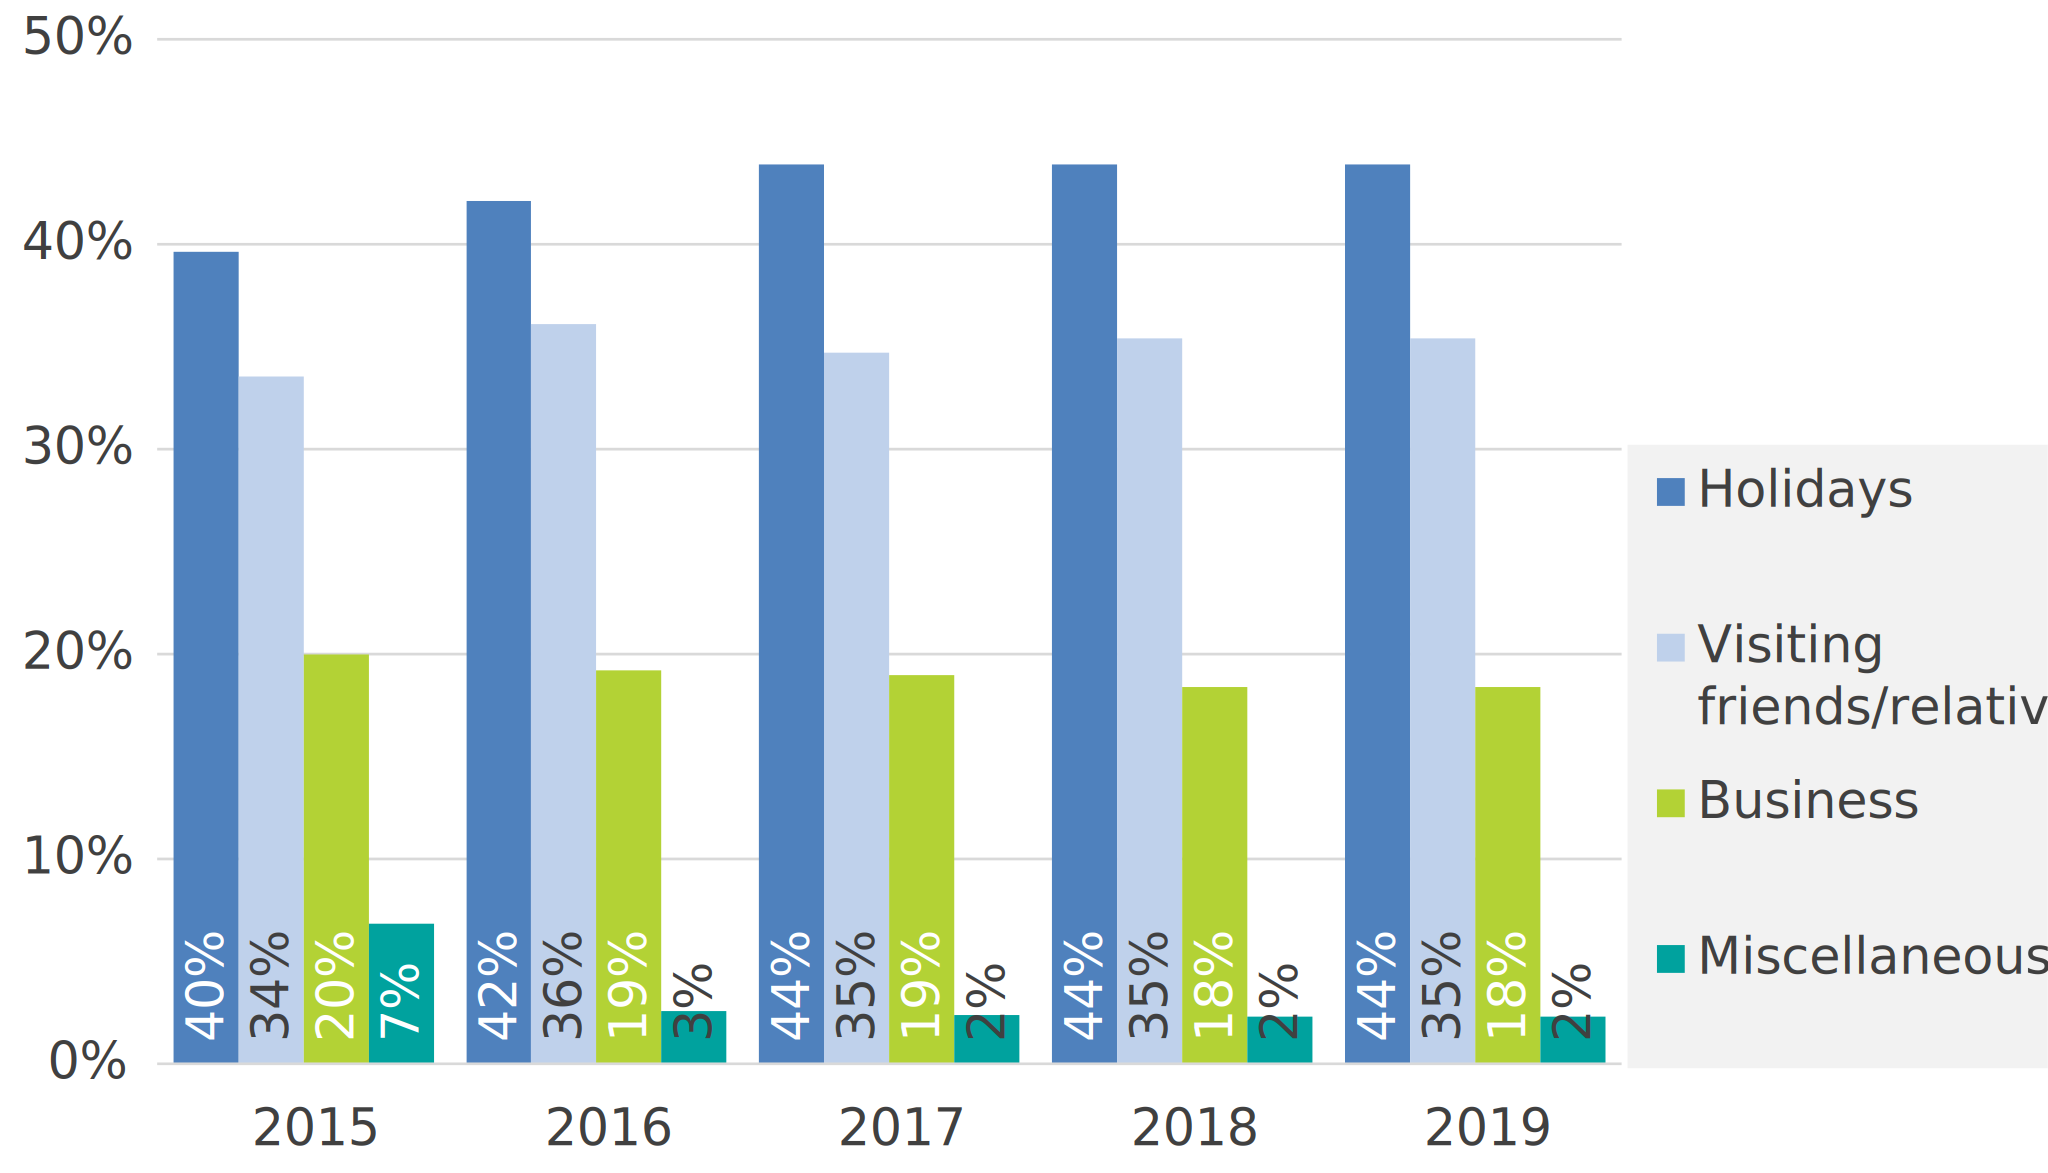
\includegraphics{chapters/../figures/travel_purpose.svg}

}

\caption{\label{fig-travel-purpose}Purpose of air passenger travel at
selected UK airports
\protect\hyperlink{ref-AviationStatistics2022}{{[}68{]}}}

\end{figure}

The results are based on the UK CAA departing passenger survey, which is
carried out at selected airports (Gatwick, Heathrow, Luton, Stansted and
Manchester), usually every year but interrupted from March 2020 onwards
due to the COVID-19 pandemic.

The scope of the statistics is travel to, from and within the UK. Over a
five-year period (2015 -- 2019).

The Holidays purpose of travel increased by 4 percentage points (p.p.)
and Visiting friends and relatives was up 2 p.p. On the other hand,
Business travel went down by 2 p.p. and Miscellaneous decreased by 5
p.p.

\hypertarget{further-reading-1}{%
\section{Further reading}\label{further-reading-1}}

Below are listed some sources recommended to consult in the frame of
this topic:

\begin{itemize}
\item
  \emph{EUROCONTROL public airport corner tool}
  \protect\hyperlink{ref-apt:corner}{{[}63{]}} provides access to
  non-confidential information relating to the purpose of travel from a
  specific airport
\item
  \emph{UK Department for Transport in its table TSGB0114b}
  \protect\hyperlink{ref-ukstats}{{[}69{]}} publishes overseas travel by
  air: visits to and from the UK by area and purpose -- all modes for
  years 2011-2019 and 2021. This data does not include domestic travel
  by air
\item
  \emph{UK Civil Aviation Authority Passenger Survey Reports}
  \protect\hyperlink{ref-paxsurvey}{{[}70{]}}
\item
  In its \emph{Yearly Compendium of Tourism Statistics},
  \protect\hyperlink{ref-untourism}{{[}71{]}} UN World Tourism
  Organisation publishes arrivals by main purpose (personal, business
  and professional)
\end{itemize}

\hypertarget{references-35}{%
\section{References}\label{references-35}}

\hypertarget{sec-passenger-value-of-time}{%
\chapter{Passenger value of time}\label{sec-passenger-value-of-time}}

\hypertarget{eurocontrol-recommended-values-34}{%
\section{EUROCONTROL recommended
values}\label{eurocontrol-recommended-values-34}}

This input provides an estimation of the average value of passenger time
spent travelling, which might alternatively be spent on other activities
(e.g.~working or leisure). It is essentially the \textbf{opportunity
cost which corresponds to the monetary value associated with a passenger
during a journey.} It shows how much a passenger would be willing to pay
in order to save time during a journey (e.g.~by travelling on a quicker
service or using a faster transport mode), or how much `compensation'
they would accept, directly or indirectly, for lost time lost.

In tables hereafter is presented a collection of the different values
that can be used for this purpose. It is to be noted that, in this
section, the value of time is not cited as a function of delay duration.
This is an important consideration when using the value. In this case,
the longer the delay duration, the higher the value.
\protect\hyperlink{ref-heatco2006}{{[}72{]}}
\protect\hyperlink{ref-frminecotra2019}{{[}73{]}}
\protect\hyperlink{ref-aptcom2014}{{[}74{]}}

\hypertarget{tbl-pas-time-value-eu}{}
\setlength{\LTpost}{0mm}
\begin{longtable}{lr}
\caption{\label{tbl-pas-time-value-eu}Estimated value of travel time - EU25 }\tabularnewline

\toprule
Travel purpose & Time value (€/hour)\textsuperscript{1} \\ 
\midrule
Personal & $\text{EUR}20.47$ \\ 
Business & $\text{EUR}49.98$ \\ 
\bottomrule
\end{longtable}
\begin{minipage}{\linewidth}
\textsuperscript{1}Please note that the values above are adjusted to 2022 prices from 2002 based on inflation\\
\emph{Source: \href{https://trimis.ec.europa.eu/sites/default/files/project/documents/20130122_113653_88902_HEATCO_D5_summary.pdf}{European Commission (2006), HEATCO, Developing Harmonised European Approaches for Transport Costing and Project Assessment -- Deliverable 5 Proposal for Harmonised Guidelines}}\\
\end{minipage}

\hypertarget{tbl-pas-time-value-fr}{}
\setlength{\LTpost}{0mm}
\begin{longtable}{lr}
\caption{\label{tbl-pas-time-value-fr}Estimated value of travel time - France }\tabularnewline

\toprule
Travel purpose & Time value (€/hour)\textsuperscript{1} \\ 
\midrule
Personal - holiday & $\text{EUR}59.80$ \\ 
Personal - other & $\text{EUR}61.20$ \\ 
Business & $\text{EUR}83.50$ \\ 
All purpose & $\text{EUR}62.10$ \\ 
\bottomrule
\end{longtable}
\begin{minipage}{\linewidth}
\textsuperscript{1}Please note that the values above are adjusted to 2022 prices from 2015 based on inflation\\
\emph{Source: \href{https://www.ecologie.gouv.fr/sites/default/files/V.3.pdf}{French Ministry of Ecological Transition (2019), Recommended values for calculating average long-distance travel}}\\
\end{minipage}

\hypertarget{tbl-pas-time-value-uk}{}
\setlength{\LTpost}{0mm}
\begin{longtable}{lr}
\caption{\label{tbl-pas-time-value-uk}Estimated value of travel time - United Kingdom }\tabularnewline

\toprule
Travel purpose & Time value (€/hour)\textsuperscript{1} \\ 
\midrule
Leisure & $\text{EUR}8.60$ \\ 
UK business & $\text{EUR}63.80$ \\ 
Foreign business & $\text{EUR}60.70$ \\ 
\bottomrule
\end{longtable}
\begin{minipage}{\linewidth}
\textsuperscript{1}Please note that the values above are adjusted to 2022 prices from 2014 based on inflation and using the exchange rate shown in general parameters\\
\emph{Source: \href{https://assets.publishing.service.gov.uk/government/uploads/system/uploads/attachment_data/file/372606/AC08a_tagged.pdf}{Airports Commission (2014), Values of time used to estimate passenger delay costs in the UK airport system}}\\
\end{minipage}

\hypertarget{when-to-use-the-input-8}{%
\section{When to use the input?}\label{when-to-use-the-input-8}}

This input is expected to become useful in any study that looks at the
opportunity cost of the use of air transport, delays, cancellations,
etc. It provides a perspective on the impact that a change in the air
transport can have on the passenger.

\hypertarget{comments-13}{%
\section{Comments}\label{comments-13}}

When looking into the values in the table, a few points regarding the
sources should be taken into consideration:

\begin{itemize}
\item
  The source used for the UK values sets out a methodology for analysis
  which has been undertaken to estimate benefits from reduced delay time
  to airlines and passengers from changes in aviation capacity
  constraints in the UK for 11 airports.
\item
  The values for France rely on a working paper on recommended values
  for calculating the components of a socio-economic net present value,
  which include travel time. The assessment therefore covers social,
  environmental and economic effects.
\item
  Regarding the numbers for EU25, they remain a reference if a European
  value is sought. The objective of the study from which they were
  derived is to propose harmonised guidelines for project assessment for
  transnational projects in Europe. It provides monetary estimates for
  the values of time saved for employer's business and for passenger
  non-work trips (e.g.~commuting, shopping and leisure).
\end{itemize}

\hypertarget{other-values-to-consider}{%
\section{Other values to consider}\label{other-values-to-consider}}

Some additional values are available to EUROCONTROL, which, although not
constituting the perceived key inputs, may be useful for specific
purposes of the user of these inputs. These values are presented below.

\textbf{\emph{Value of time of a business aviation passenger}}

\textbf{€153 per hour.} This value was provided to EUROCONTROL by
airline members of the SESAR CBA team in 2012 and is, therefore,
adjusted from 2011 prices.

\textbf{\emph{Value of passenger time in the US for high-speed rail
passengers}}

Based on US DOT guidance on passenger value of time for air and
high-speed rail travel by purpose of trip. The numbers are adjusted to
inflation from 2015 prices and using the exchange rate presented in
Table~\ref{tbl-eurostat-exchange-rates}.

\hypertarget{further-reading-2}{%
\section{Further reading}\label{further-reading-2}}

Below are listed some additional sources recommended for consultation:

\begin{itemize}
\item
  International Transport Forum (ITF), ``What is the Value of Saving
  Travel Time?'' Feb.~2019\protect\hyperlink{ref-itf:2019}{{[}75{]}}
\item
  Economic Development Research Group Inc., ``Passenger Value of Time,
  Benefit-Cost Analysis and Airport Capital Investment Decisions,''
  2015\protect\hyperlink{ref-passtimevalue2015}{{[}76{]}}
\item
  University of Leeds, ``Values of travel time in Europe: Review and
  meta-analysis,''
  2016\protect\hyperlink{ref-leedsuniversity2016}{{[}77{]}}
\item
  University of Leeds, ``European Wide-Meta Analysis of Values of Travel
  Time,'' May 2012\protect\hyperlink{ref-leedsuniversity2012}{{[}78{]}}
\end{itemize}

\hypertarget{references-36}{%
\section{References}\label{references-36}}

\part{Safety}

\hypertarget{sec-accident-incident-statistics}{%
\chapter{Accident/incident
statistics}\label{sec-accident-incident-statistics}}

\hypertarget{eurocontrol-recommended-sources-4}{%
\section{EUROCONTROL recommended
sources}\label{eurocontrol-recommended-sources-4}}

Hereafter are presented some sources that are recommended to be
consulted to obtain latest statistics on accidents and incidents
occurring in the aviation domain, as well as the related fatalities and
injuries.

According to \textbf{ICAO Annex 13:}

An \textbf{accident} is an occurrence associated with the operation of
an aircraft \ldots, in which (a) a person is fatally or seriously
injured\ldots{} or (b) the aircraft sustains damage or structural
failure \ldots or (c) the aircraft is missing or completely inaccessible
.

An \textbf{incident} is an occurrence, other than an accident,
associated with the operation of an aircraft which affects or could
affect the safety of operations.

The key sources are:

\begin{itemize}
\item
  \textbf{EASA Annual Safety Review}
  \protect\hyperlink{ref-AnnualSafetyReview}{{[}79{]}} provides both, a
  statistical summary of aviation safety in the EASA Member States and
  identifies the most important safety challenges faced by European
  aviation today. The key statistics on accidents and serious incidents
  in the different aviation domains can be found at the start of each
  chapter in the Annual Safety Review.
\item
  \textbf{EUROCONTROL voluntary ATM incident reporting (EVAIR) safety
  bulletin} \protect\hyperlink{ref-atmincidentreport}{{[}80{]}} collects
  low-severity ATM incidents which involve pilots and controllers. The
  established process and kinds of data provided by airlines and ANSP
  SMS allow day to day analysis and, in this regard, identification of
  the causes of incidents. The data are collected from the entire ECAC
  region and from neighbouring airspace, such as the Eastern part of the
  ICAO EUR region, the Middle East, Africa, etc.
\item
  \textbf{IATA Annual Safety Report}
  \protect\hyperlink{ref-iata:safety:report}{{[}81{]}} provides the
  industry with critical information derived from the analysis of
  aviation accidents to enable to understand safety risks in the
  industry and to propose mitigation strategies.
\end{itemize}

\hypertarget{when-to-use-the-input-9}{%
\section{When to use the input?}\label{when-to-use-the-input-9}}

This input is recommended to be used in the instances where the safety
is an important factor, namely in terms of accident reduction.

\hypertarget{further-reading-3}{%
\section{Further reading}\label{further-reading-3}}

The sources listed hereafter are those recommended to consult for
further information:

\begin{itemize}
\item
  \emph{EU Regulation (EU) No 996/2010 on the investigation and
  prevention of accidents and incidents in civil aviation and repealing
  Directive 94/56/EC} \protect\hyperlink{ref-eureg9962010}{{[}82{]}}
  contains a definition of accidents and incidents
\item
  \emph{EU Regulation (EU) No 376/2014 on the reporting, analysis and
  follow-up of occurrences in civil aviation, amending Regulation (EU)
  No 996/2010 of the European Parliament and of the Council and
  repealing Directive 2003/42/EC of the European Parliament and of the
  Council and Commission Regulations (EC) No 1321/2007 and (EC) No
  1330/2007} \protect\hyperlink{ref-eureg3762014}{{[}83{]}} contains
  information on the regulatory requirements reporting, analysis and
  follow-up of occurrences, which include accidents and incidents in
  civil aviation
\item
  \emph{EU Single Sky Performance Review Body, Annual Monitoring Report}
  \protect\hyperlink{ref-EUSingleSky}{{[}84{]}} The Annual Monitoring
  Reports are prepared by the Performance Review Body (PRB) of the
  Single European Sky (SES)
\item
  \emph{ICAO safety reports}
  \protect\hyperlink{ref-icao:safety}{{[}85{]}} reports on worldwide
  aviation safety performance and collaborative efforts by international
  air transport stakeholders to further improve safety in light of the
  sustained growth of the sector
\item
  \emph{Performance Review Commission (2022) Draft Performance Review
  Report (PRR) 2022 for consultation}
  \protect\hyperlink{ref-ectrlprr2022}{{[}43{]}} Annual Performance
  Review Reports issued by the Performance Review Commission provide an
  annual review of Europe's ATM safety performance
\item
  \emph{SKYbrary} \protect\hyperlink{ref-SkyBrary}{{[}86{]}} An
  electronic repository of safety knowledge related to ATM and aviation
  safety in general. It contains information about accidents and serious
  incidents by aircraft type and is also a portal which gives users
  access to the safety data made available on the websites of various
  aviation organisations (regulators, service providers, industry)
\end{itemize}

\hypertarget{references-37}{%
\section{References}\label{references-37}}

\hypertarget{sec-value-of-a-statistical-life}{%
\chapter{Value of a statistical
life}\label{sec-value-of-a-statistical-life}}

\hypertarget{eurocontrol-recommended-values-35}{%
\section{EUROCONTROL recommended
values}\label{eurocontrol-recommended-values-35}}

Value of a Statistical Life (VSL) represents the monetary willingness to
pay for a lower risk of instantaneous premature death. It is often used
as a proxy to monetise the value of a fatality occurring form transport
accidents.

In Europe, based on a study published by the European
Commission\protect\hyperlink{ref-ecdgmove2019}{{[}27{]}} the
\textbf{average statistical value of life for EU27+UK is estimated at €
4.3 million.} This value is adjusted to 2022 prices from 2016, based on
inflation.

It is to note that the value of life differs based on the country,
circumstances, age, profession, education and a number of other
parameters. It also differs for different modes of transport. Thus,
different
sources{[}\protect\hyperlink{ref-easa2013}{{[}87{]}}{]}\protect\hyperlink{ref-ecdgregio2014}{{[}58{]}}\protect\hyperlink{ref-ecbr2021}{{[}88{]}}
propose different values and ways to estimate them, depending on
specific circumstances.

\hypertarget{when-to-use-the-input-10}{%
\section{When to use the input?}\label{when-to-use-the-input-10}}

This input is recommended to be used in studies where the cost of
fatalities resulting from safety accidents in aviation needs to be
monetised. This is a significant part of an economic impact of a
solution, particularly when the solution focuses on safety improvement.

\hypertarget{related-inputs-27}{%
\section{Related inputs}\label{related-inputs-27}}

Chapter~\ref{sec-accident-incident-statistics}
\protect\hyperlink{sec-accident-incident-statistics}{Accident/incident
statistics}

Chapter~\ref{sec-value-of-statistical-injury}
\protect\hyperlink{sec-value-of-statistical-injury}{Value of a
statistical injury}

\hypertarget{references-38}{%
\section{References}\label{references-38}}

\hypertarget{sec-value-of-statistical-injury}{%
\chapter{Value of a statistical
injury}\label{sec-value-of-statistical-injury}}

The value of a statistical injury represents the \textbf{monetary value
of an improvement in safety to achieve a risk reduction which would
prevent one statistical injury.} It can be used as a proxy to monetise
the impact of an injury resulting from transport accidents.

Table~\ref{tbl-value-of-injury} shows the estimation of the value of an
injury as a fraction of the
\protect\hyperlink{sec-value-of-a-statistical-life}{value of statistical
life}, following the approach and numbers presented in the Handbook on
the external costs of
transport.\protect\hyperlink{ref-ecdgmove2019}{{[}27{]}} This approach
assumes six levels of injury, where Maximum Abbreviated Injury Scale
(MAIS) 1 and MAIS 2 represent slight injury, MAIS 3 through MAIS 5
represent serious injury and MAIS 6 represents fatality.

Thus, in Table~\ref{tbl-value-of-injury} are presented the levels of
injury, the share that the value of injury represents from the value of
life and the calculated cost of injury in euros, based on these
percentages and the estimated value of statistical life as presented in
Chapter~\ref{sec-value-of-a-statistical-life}.

\hypertarget{tbl-value-of-injury}{}
\setlength{\LTpost}{0mm}
\begin{longtable}{lcr}
\caption{\label{tbl-value-of-injury}Estimated value of statistical injury }\tabularnewline

\toprule
Injury category & Share of VSL & Value of injury \\ 
\midrule
MAIS 1 & $0\%$ & $\text{EUR}12,900$ \\ 
MAIS 2 & $4\%$ & $\text{EUR}189,200$ \\ 
MAIS 3 & $10\%$ & $\text{EUR}447,200$ \\ 
MAIS 4 & $26\%$ & $\text{EUR}1,130,900$ \\ 
MAIS 5 & $59\%$ & $\text{EUR}2,541,300$ \\ 
MAIS 6 (fatality) & $100\%$ & $\text{EUR}4,300,000$ \\ 
\bottomrule
\end{longtable}
\begin{minipage}{\linewidth}
\emph{\href{https://op.europa.eu/en/publication-detail/-/publication/9781f65f-8448-11ea-bf12-01aa75ed71a1}{Source: European Commission DG MOVE (2019), Handbook on the external costs of transport}}\\
\end{minipage}

\hypertarget{comments-14}{%
\section{Comments}\label{comments-14}}

The above data should be treated with caution as there may be legal
implications.

\hypertarget{other-possible-sources-7}{%
\section{Other possible sources}\label{other-possible-sources-7}}

Below are presented some sources recommended to be consulted in the
frame of this input:

\emph{European Commission DG REGIO, Guide to Cost-Benefit Analysis of
Investment Projects for Cohesion Policy
2014-2020}\protect\hyperlink{ref-ecdgregio2014}{{[}58{]}}

\hypertarget{related-inputs-28}{%
\section{Related inputs}\label{related-inputs-28}}

Chapter~\ref{sec-accident-incident-statistics}
\protect\hyperlink{sec-accident-incident-statistics}{Accident/incident
statistics}

Chapter~\ref{sec-value-of-a-statistical-life}
\protect\hyperlink{sec-value-of-a-statistical-life}{Value of a
statistical life}

\hypertarget{references-39}{%
\section{References}\label{references-39}}

\part{Financial values}

\hypertarget{sec-discount-rate}{%
\chapter{Discount rate}\label{sec-discount-rate}}

\hypertarget{eurocontrol-recommended-value-2}{%
\section{EUROCONTROL recommended
value}\label{eurocontrol-recommended-value-2}}

Discount rate is the annual rate used to discount a stream of cashflows
in order to calculate their Net Present Value (NPV).

The \textbf{discount rate recommended to be used for the EU is
4\%.}\footnote{\href{https://eur-lex.europa.eu/legal-content/EN/TXT/?uri=uriserv\%3AOJ.L_.2014.138.01.0005.01.ENG}{European
  Commission (2014), Commission Delegated Regulation (EU) No 480/2014,
  Article 19 (Discounting of Cash Flow)}}

\hypertarget{description-16}{%
\section{Description}\label{description-16}}

A nominal discount rate has three components:

\begin{itemize}
\item
  a basic, risk-free, time value of money (TVM) -- traditionally of the
  order of 2.5\%
\item
  compensation for the erosion of the principal by inflation
\item
  a premium for risk
\end{itemize}

The inflation element should only be included if the cash flows are
expressed in `money of the day' and should be excluded if the cash flows
are expressed at constant price levels. The recommended value is
inflation-free and only takes into account TVM and the risk premium.

The assessment of the risk premium depends on the judgment of the
investor and can only be analysed over a portfolio of investments. In
the case of investment in an air traffic management system, the risk
being evaluated is the risk that the system will operate successfully
and generate the benefits expected. It is not related to the commercial
viability of aircraft operators using the system.

The value is used as an indicative benchmark in (EUROCONTROL) business
cases for ATM investments and is applied to costs incurred and benefits
achieved by air navigation service providers, aircraft operators and any
other parties involved.

Values differing from the 4\% benchmark can, however, be justified on
the grounds of local and individual conditions which affect the
requisite risk premium.

\hypertarget{other-recommended-values}{%
\section{Other recommended values}\label{other-recommended-values}}

Another way to calculate the discount rate is by using the Weighted Cost
of Capital (WACC) metric. According to Implementing Regulation 2019/317
art. 22 (4),\protect\hyperlink{ref-ir2019317}{{[}89{]}} WACC is defined
as the average of the return on equity and the interest rate on debt,
weighted by the capital structure. According to the same source, the
WACC relevant for the assessment of performance plans is the cost of
capital pre-tax rate.

In their Study on cost of capital, methodology review and update report,
\protect\hyperlink{ref-prb2021}{{[}90{]}} the Performance Review Body
(PRB) of the Single European Sky performed an assessment of the cost of
capital for the ANSPs of the Single European Sky Member States.

The methodological approach taken by PRB calculates efficient costs of
capital and combines them with a check on the maximum exposure due to
the traffic-risk sharing mechanism.\footnote{Please refer to the source
  document for further details} The cost of capital is assessed
according to four options\footnote{See table 2 of the source document}\\
that are summarised as follows:

\begin{itemize}
\item
  \textbf{Option 1} should be used when the WACC of an ANSP is based on
  an actual capital structure that is not aligned to the optimal capital
  structure
\item
  \textbf{Option 2} should be used if it is lower than Option 1 for an
  ANSP that is subject to a government-specified equity return
\item
  \textbf{Option 3} should be used if it is lower than Option 1 for an
  ANSP that has access to loan finance on favourable terms but is not
  subject to a government-specified equity return
\item
  \textbf{Option 4} is an additional sense check of the cost of capital
  (the WACC times the asset base) and the maximum risk exposure of the
  ANSP (4.4\% of revenues)
\end{itemize}

Option 1 is used as a reference here because it constitutes the baseline
value in the study, while the remaining three options are subject to
specific circumstances described above.

As a result of this assessment, the \textbf{average estimated pre-tax
WACC in 2022 for all Member States' ANSPs for option 1 amounts 4.6\%.}

According to PRB, Options 2-4 of the methodological framework may result
in lower numbers than Option 1 if the ANSP is subject to a lower
government-specified return on equity (Option 2), if the ANSP obtains
loan finance on more favourable terms (Option 3), or if the WACC implied
by the maximum exposure of the ANSP is lower (Option 4).

\hypertarget{further-reading-4}{%
\section{Further reading}\label{further-reading-4}}

The sources listed below are those recommended to consult for further
information about discount rate:

\begin{itemize}
\item
  \emph{European Commission (2021), Better regulation
  toolbox}\protect\hyperlink{ref-ecbr2021}{{[}88{]}} has been created to
  support designing EU policies and laws so that they achieve their
  objectives at minimum cost. The Guidelines explain what better
  regulation is and how it should be applied in the day-to-day practices
  of Commission officials preparing new initiatives and proposals or
  managing existing policies and legislation
\item
  \emph{European Commission (2014), Guide to Cost-Benefit Analysis of
  Investment projects, Economic appraisal tool for Cohesion policy
  2014-2020} \protect\hyperlink{ref-ecdgregio2014}{{[}58{]}} offers
  practical guidance on major project appraisals, as embodied in the
  cohesion policy legislation for 2014-2020 and takes into account the
  specific requirements for the European Commission
\item
  \emph{European Commission (2021), Economic Appraisal Vademecum
  2021-2027 -- General principles and sector applications}
  \protect\hyperlink{ref-ecdgregiovademecum2022}{{[}59{]}} Further
  promotes and simplifies the voluntary use of Economic Appraisal for EU
  co-financed investments in the 2021-2027 programming period
\item
  \emph{GOV.UK, HM Treasury (2018), The Green Book: Central Government
  Guidance on Appraisal and Evaluation}
  \protect\hyperlink{ref-greenbook:2018}{{[}91{]}} The EUROCONTROL
  recommended value of 4\% is not suitable for discounting
  intergenerational projects, especially the projects dealing with
  environmental matters. A declining long-term discount rate approach
  may be used following the example on p.104 of this document
\end{itemize}

\hypertarget{comments-15}{%
\section{Comments}\label{comments-15}}

Different approaches to determining discount rates can be used (social
rate of time preference, marginal social opportunity cost of capital,
weighted average cost of capital, shadow price of capital). A
description of these approaches goes beyond the limits of this document.

The choice of an appropriate social discount rate for the cost-benefit
analysis of public projects has long been a contentious issue and
subject to intense debate by economists.

Since the choice of discount rate is a matter of judgment, it is
recommended that in project appraisals the sensitivity analysis should
include a consideration of the effect of differing discount rates. Note
that the Internal Rate of Return (IRR) is the discount rate which will
give an NPV of zero and thus gives the effective overall return on an
investment over the period under consideration.

\hypertarget{references-40}{%
\section{References}\label{references-40}}

\hypertarget{sec-exchange-rate}{%
\chapter{Exchange rate}\label{sec-exchange-rate}}

\hypertarget{eurocontrol-recommended-source}{%
\section{EUROCONTROL recommended
source}\label{eurocontrol-recommended-source}}

Exchange rate represents the price or rate at which the currency of a
country can be exchanged for another country's currency.

In order to obtain the latest exchange rate information it is
recommended to vist the website of the
\href{http://sdw.ecb.europa.eu/}{European Central Bank}.

The website contains information on the yearly, half-yearly, quarterly,
monthly and daily exchange rates of 40 currencies.

As an alternative, the European Commission
\href{https://commission.europa.eu/funding-tenders/procedures-guidelines-tenders/information-contractors-and-beneficiaries/exchange-rate-inforeuro_en}{InforEuro}
Exchange rate provides the European Commission official monthly
accounting rates for the euro, the corresponding conversion rates for
other currencies, and historic conversion rates from 1994.

\hypertarget{refs}{}
\begin{CSLReferences}{0}{0}
\leavevmode\vadjust pre{\hypertarget{ref-eurostat:HICP}{}}%
\CSLLeftMargin{{[}1{]} }%
\CSLRightInline{Eurostat, {``Harmonised {Indices} of {Consumer Prices}
({HICP}).''} {[}Online{]}. Available:
\url{https://ec.europa.eu/eurostat/web/hicp}. {[}Accessed: Dec. 12,
2022{]}}

\leavevmode\vadjust pre{\hypertarget{ref-ECB:exchange_rates}{}}%
\CSLLeftMargin{{[}2{]} }%
\CSLRightInline{European Central Bank, {``Euro foreign exchange
reference rates,''} \emph{European Central Bank}. Mar. 2022
{[}Online{]}. Available:
\url{https://www.ecb.europa.eu/stats/policy_and_exchange_rates/euro_reference_exchange_rates/html/index.en.html}.
{[}Accessed: Dec. 12, 2022{]}}

\leavevmode\vadjust pre{\hypertarget{ref-iata:JetFuelPrice}{}}%
\CSLLeftMargin{{[}3{]} }%
\CSLRightInline{IATA, {``Jet {Fuel Price Monitor}.''} {[}Online{]}.
Available:
\url{https://www.iata.org/en/publications/economics/fuel-monitor/}.
{[}Accessed: Dec. 12, 2022{]}}

\leavevmode\vadjust pre{\hypertarget{ref-statfor:7year_forecast:2022-2028}{}}%
\CSLLeftMargin{{[}4{]} }%
\CSLRightInline{STATFOR, {``{EUROCONTROL Forecast Update} 2022-2028.''}
{[}Online{]}. Available:
\url{https://www.eurocontrol.int/publication/eurocontrol-forecast-update-2022-2028}.
{[}Accessed: Dec. 12, 2022{]}}

\leavevmode\vadjust pre{\hypertarget{ref-ectrl:statfor:sid}{}}%
\CSLLeftMargin{{[}5{]} }%
\CSLRightInline{EUROCONTROL STATFOR, {``{STATFOR Interactive
Dashboard}.''} {[}Online{]}. Available:
\url{https://www.eurocontrol.int/dashboard/statfor-interactive-dashboard}}

\leavevmode\vadjust pre{\hypertarget{ref-aviation:outlook2022}{}}%
\CSLLeftMargin{{[}6{]} }%
\CSLRightInline{EUROCONTROL, {``{EUROCONTROL Aviation Outlook} 2050,''}
Apr. 2022 {[}Online{]}. Available:
\url{https://www.eurocontrol.int/publication/eurocontrol-aviation-outlook-2050}}

\leavevmode\vadjust pre{\hypertarget{ref-ectrl:nop:2022}{}}%
\CSLLeftMargin{{[}7{]} }%
\CSLRightInline{EUROCONTROL NMD, {``European {Network Operations Plan}
2022-2026,''} Jul. 2022 {[}Online{]}. Available:
\url{https://www.eurocontrol.int/publication/european-network-operations-plan-2022-2026}}

\leavevmode\vadjust pre{\hypertarget{ref-ectrl:nop:rsp}{}}%
\CSLLeftMargin{{[}8{]} }%
\CSLRightInline{EUROCONTROL NMD, {``European {Network Operations Plan}
2023 {Rolling Seasonal Plan}''} {[}Online{]}. Available:
\url{https://www.eurocontrol.int/publication/european-network-operations-plan-2022-rolling-seasonal-plan}}

\leavevmode\vadjust pre{\hypertarget{ref-ectrl:mp:ip}{}}%
\CSLLeftMargin{{[}9{]} }%
\CSLRightInline{EUROCONTROL, {``European {ATM Master Plan} -
implementation plan - level 3,''} Dec. 2022 {[}Online{]}. Available:
\url{https://www.eurocontrol.int/publication/european-atm-master-plan-implementation-plan-level-3}}

\leavevmode\vadjust pre{\hypertarget{ref-ectrl:mp:ir}{}}%
\CSLLeftMargin{{[}10{]} }%
\CSLRightInline{EUROCONTROL, {``European {ATM Master Plan} -
implementation report- level 3,''} Aug. 2022 {[}Online{]}. Available:
\url{https://www.eurocontrol.int/publication/european-atm-master-plan-implementation-report-level-3}}

\leavevmode\vadjust pre{\hypertarget{ref-ectrl:lssip}{}}%
\CSLLeftMargin{{[}11{]} }%
\CSLRightInline{EUROCONTROL, {``Local {Single Sky} implementation
monitoring.''} {[}Online{]}. Available:
\url{https://www.eurocontrol.int/service/local-single-sky-implementation-monitoring}}

\leavevmode\vadjust pre{\hypertarget{ref-ectl:market:seg:2022}{}}%
\CSLLeftMargin{{[}12{]} }%
\CSLRightInline{EUROCONTROL, {``{EUROCONTROL Market Segment Update}
2022,''} May 2022 {[}Online{]}. Available:
\url{https://www.eurocontrol.int/publication/market-segment-rules}}

\leavevmode\vadjust pre{\hypertarget{ref-prb:dashboard:2022}{}}%
\CSLLeftMargin{{[}13{]} }%
\CSLRightInline{{``Reporting {Period} 3 - 2021 dashboard.''} 2022
{[}Online{]}. Available:
\url{https://www.eurocontrol.int/prudata/dashboard/vis/2021/}}

\leavevmode\vadjust pre{\hypertarget{ref-coda2021}{}}%
\CSLLeftMargin{{[}14{]} }%
\CSLRightInline{C. Walker, {``All-causes delay and cancellations to air
transport in {Europe} -- {Annual} report for 2021,''} {EUROCONTROL
CODA}, Mar. 2022 {[}Online{]}. Available:
\url{https://www.eurocontrol.int/sites/default/files/2022-04/eurocontrol-coda-digest-annual-report-2021.pdf}.
{[}Accessed: Nov. 26, 2022{]}}

\leavevmode\vadjust pre{\hypertarget{ref-nm2022}{}}%
\CSLLeftMargin{{[}15{]} }%
\CSLRightInline{{``Network operations report 2021,''} {EUROCONTROL}, May
2022 {[}Online{]}. Available:
\url{https://www.eurocontrol.int/sites/default/files/2022-05/eurocontrol-annual-nor-2021-main-report.pdf}}

\leavevmode\vadjust pre{\hypertarget{ref-ectllibrary}{}}%
\CSLLeftMargin{{[}16{]} }%
\CSLRightInline{EUROCONTROL, {``{EUROCONTROL Library}.''} {[}Online{]}.
Available: \url{https://www.eurocontrol.int/library}}

\leavevmode\vadjust pre{\hypertarget{ref-aiuportal}{}}%
\CSLLeftMargin{{[}17{]} }%
\CSLRightInline{EUROCONTROL AIU, {``{AIU} portal.''} {[}Online{]}.
Available: \url{https://ansperformance.eu/data/}. {[}Accessed: Dec. 01,
2022{]}}

\leavevmode\vadjust pre{\hypertarget{ref-ace2019}{}}%
\CSLLeftMargin{{[}18{]} }%
\CSLRightInline{EUROCONTROL PRU, {``Air traffic management
cost-effectiveness ({ACE}) benchmarking report for 2019,''}
{EUROCONTROL}, May 2021 {[}Online{]}. Available:
\url{https://www.eurocontrol.int/publication/air-traffic-management-cost-effectiveness-ace-benchmarking-report-2019}}

\leavevmode\vadjust pre{\hypertarget{ref-emissionscalc}{}}%
\CSLLeftMargin{{[}19{]} }%
\CSLRightInline{ICAO, {``Carbon {Emissions Calculator}.''} {[}Online{]}.
Available:
\url{https://www.icao.int/environmental-protection/Carbonoffset/Pages/default.aspx}}

\leavevmode\vadjust pre{\hypertarget{ref-ectrl:em:model}{}}%
\CSLLeftMargin{{[}20{]} }%
\CSLRightInline{EUROCONTROL, {``Advanced emission model.''}
{[}Online{]}. Available:
\url{https://www.eurocontrol.int/model/advanced-emission-model}}

\leavevmode\vadjust pre{\hypertarget{ref-icao:databank}{}}%
\CSLLeftMargin{{[}21{]} }%
\CSLRightInline{ICAO, {``Engine {Emissions Databank}.''} {[}Online{]}.
Available:
\url{https://www.easa.europa.eu/en/domains/environment/icao-aircraft-engine-emissions-databank}}

\leavevmode\vadjust pre{\hypertarget{ref-SESAR2020Environment}{}}%
\CSLLeftMargin{{[}22{]} }%
\CSLRightInline{SESAR 2020, \emph{{SESAR} 2020 \textendash{}
{Environment Impact Assessment Guidance Del}: 4.0.080}. }

\leavevmode\vadjust pre{\hypertarget{ref-eaer2022}{}}%
\CSLLeftMargin{{[}23{]} }%
\CSLRightInline{EUROCONTROL, EASA, EU, {``European {Aviation
Environmental Report} 2022,''} Sep. 2022 {[}Online{]}. Available:
\url{https://www.eurocontrol.int/publication/european-aviation-environmental-report-2022}}

\leavevmode\vadjust pre{\hypertarget{ref-eea:2019}{}}%
\CSLLeftMargin{{[}24{]} }%
\CSLRightInline{European Environment Agency, {``{EMEP}/{EEA} air
pollutant emission inventory guidebook 2019,''} 2019 {[}Online{]}.
Available:
\url{https://www.eea.europa.eu/publications/emep-eea-guidebook-2019}}

\leavevmode\vadjust pre{\hypertarget{ref-foca:aee}{}}%
\CSLLeftMargin{{[}25{]} }%
\CSLRightInline{Swiss Federal Office of Civil Aviation, {``Aircraft
{Engine Emissions}''} {[}Online{]}. Available:
\url{https://www.bazl.admin.ch/bazl/en/home.html}}

\leavevmode\vadjust pre{\hypertarget{ref-envimpact}{}}%
\CSLLeftMargin{{[}26{]} }%
\CSLRightInline{Swedish Defence Research Agency, {``The {Environmental
Impact} of {Aircraft}''} {[}Online{]}. Available:
\url{https://www.foi.se/en/foi/research/aeronautics-and-space-issues/environmental-impact-of-aircraft.html}}

\leavevmode\vadjust pre{\hypertarget{ref-ecdgmove2019}{}}%
\CSLLeftMargin{{[}27{]} }%
\CSLRightInline{European Commission DG MOVE, {``Handbook on the external
costs of transport,''} 2019 {[}Online{]}. Available:
\url{https://op.europa.eu/en/publication-detail/-/publication/9781f65f-8448-11ea-bf12-01aa75ed71a1}}

\leavevmode\vadjust pre{\hypertarget{ref-ecc:limateaction}{}}%
\CSLLeftMargin{{[}28{]} }%
\CSLRightInline{European Commission, {``European {Commission Climate
Action}.''} {[}Online{]}. Available:
\url{https://ec.europa.eu/clima/policies/ets/auctioning_en}}

\leavevmode\vadjust pre{\hypertarget{ref-defra:2020}{}}%
\CSLLeftMargin{{[}29{]} }%
\CSLRightInline{DEFRA, \emph{Air quality damage cost update 2020}. 2020
{[}Online{]}. Available:
\url{https://uk-air.defra.gov.uk/library/reports?report_id=1006}}

\leavevmode\vadjust pre{\hypertarget{ref-GuidanceNoisePollution}{}}%
\CSLLeftMargin{{[}30{]} }%
\CSLRightInline{UK Department for Environment, Food \& Rural Affairs,
{``Guidance. {Noise} pollution: Economic analysis.''} {[}Online{]}.
Available:
\url{https://www.gov.uk/guidance/noise-pollution-economic-analysis}}

\leavevmode\vadjust pre{\hypertarget{ref-eib2020}{}}%
\CSLLeftMargin{{[}31{]} }%
\CSLRightInline{European Investment Bank, {``{EIB Group Climate Bank
Roadmap} 2021-2025,''} Nov. 2020 {[}Online{]}. Available:
\url{https://www.eib.org/en/publications/the-eib-group-climate-bank-roadmap}}

\leavevmode\vadjust pre{\hypertarget{ref-ipcc2018}{}}%
\CSLLeftMargin{{[}32{]} }%
\CSLRightInline{IPCC, {``Global {Warming} of 1.5
{\textordmasculine C},''} 2018 {[}Online{]}. Available:
\url{https://www.ipcc.ch/sr15/}}

\leavevmode\vadjust pre{\hypertarget{ref-easa:Fit55ReFuelEU}{}}%
\CSLLeftMargin{{[}33{]} }%
\CSLRightInline{{``Fit for 55 and {ReFuelEU Aviation},''} \emph{EASA}.
{[}Online{]}. Available:
\url{https://www.easa.europa.eu/en/light/topics/fit-55-and-refueleu-aviation}.
{[}Accessed: Dec. 12, 2022{]}}

\leavevmode\vadjust pre{\hypertarget{ref-skygreen2022}{}}%
\CSLLeftMargin{{[}34{]} }%
\CSLRightInline{EUROCONTROL, {``Objective {Skygreen} 2022-2030. {The}
economics of aviation decarbonisation towards te 2030 {Green Deal}
milestone,''} May 2022 {[}Online{]}. Available:
\url{https://www.eurocontrol.int/publication/objective-skygreen-2022-2030}}

\leavevmode\vadjust pre{\hypertarget{ref-ectl:asu}{}}%
\CSLLeftMargin{{[}35{]} }%
\CSLRightInline{EUROCONTROL ASU, {``Aviation sustainability,''}
\emph{Aviation sustainability}. {[}Online{]}. Available:
\url{https://www.eurocontrol.int/aviation-sustainability}}

\leavevmode\vadjust pre{\hypertarget{ref-iata:cmg}{}}%
\CSLLeftMargin{{[}36{]} }%
\CSLRightInline{{``{IATA Airline Cost Management Group}.''}
{[}Online{]}. Available:
\url{https://www.iata.org/en/services/finance/airline-cost-mgmt/}}

\leavevmode\vadjust pre{\hypertarget{ref-eureg2612004}{}}%
\CSLLeftMargin{{[}37{]} }%
\CSLRightInline{European Commission, {``Regulation ({EC}) {No} 261/2004
of the {European Parliament} and of the {Council} of 11 {February} 2004
establishing common rules on compensation and assistance to passengers
in the event of denied boarding and of cancellation or long delay of
flights, and repealing {Regulation} ({EEC}) {No} 295/91.''}
{[}Online{]}. Available:
\url{https://eur-lex.europa.eu/legal-content/EN/TXT/?uri=CELEX\%3A32004R0261\#:~:text=Regulation\%20\%28EC\%29\%20No\%20261\%2F2004\%20of\%20the\%20European\%20Parliament,of\%20flights\%2C\%20and\%20repealing\%20Regulation\%20\%28EEC\%29\%20No\%20295\%2F91}}

\leavevmode\vadjust pre{\hypertarget{ref-eureg:3902013}{}}%
\CSLLeftMargin{{[}38{]} }%
\CSLRightInline{European Commission, {``Commission {Implementing
Regulation} ({EU}) {No} 390/2013 of 3 {May} 2013 laying down a
performance scheme for air navigation services and network functions
{Text} with {EEA} relevance.''} 2013 {[}Online{]}. Available:
\url{https://eur-lex.europa.eu/legal-content/EN/TXT/?uri=CELEX:32013R0390\#:~:text=Commission\%20Implementing\%20Regulation\%20\%28EU\%29\%20No\%20390\%2F2013\%20of\%203,services\%20and\%20network\%20functions\%20Text\%20with\%20EEA\%20relevance.}}

\leavevmode\vadjust pre{\hypertarget{ref-uow:2004}{}}%
\CSLLeftMargin{{[}39{]} }%
\CSLRightInline{University of Westminster, {``Evaluating the true cost
to airlines of one minute of airborne or ground delay,''} 2004
{[}Online{]}. Available:
\url{https://www.eurocontrol.int/publication/evaluating-true-cost-airlines-one-minute-airborne-or-ground-delay}}

\leavevmode\vadjust pre{\hypertarget{ref-uow:2015}{}}%
\CSLLeftMargin{{[}40{]} }%
\CSLRightInline{University of Westminster, {``European airline delay
cost reference values - version 4.1,''} 2015 {[}Online{]}. Available:
\url{https://www.eurocontrol.int/publication/european-airline-delay-cost-reference-values}}

\leavevmode\vadjust pre{\hypertarget{ref-coda:mirror}{}}%
\CSLLeftMargin{{[}41{]} }%
\CSLRightInline{EUROCONTROL CODA, {``{MIRROR} tool.''} {[}Online{]}.
Available: \url{https://www.eurocontrol.int/tool/mirror}}

\leavevmode\vadjust pre{\hypertarget{ref-ectrlprr2021}{}}%
\CSLLeftMargin{{[}42{]} }%
\CSLRightInline{EUROCONTROL, {``Performance {Review Report} ({PRR})
2020,''} 2021 {[}Online{]}. Available:
\url{https://www.eurocontrol.int/publication/performance-review-report-prr-2021}.
{[}Accessed: Sep. 03, 2023{]}}

\leavevmode\vadjust pre{\hypertarget{ref-ectrlprr2022}{}}%
\CSLLeftMargin{{[}43{]} }%
\CSLRightInline{EUROCONTROL, {``Performance {Review Report} ({PRR})
2021,''} 2022 {[}Online{]}. Available:
\url{https://www.eurocontrol.int/publication/performance-review-report-prr-2021}.
{[}Accessed: Sep. 03, 2023{]}}

\leavevmode\vadjust pre{\hypertarget{ref-ectl:bada}{}}%
\CSLLeftMargin{{[}44{]} }%
\CSLRightInline{EUROCONTROL, {``Base of aircraft data ({BADA}).''}
{[}Online{]}. Available: \url{https://www.eurocontrol.int/model/bada}}

\leavevmode\vadjust pre{\hypertarget{ref-ace2020}{}}%
\CSLLeftMargin{{[}45{]} }%
\CSLRightInline{EUROCONTROL PRU, {``Air traffic management
cost-effectiveness ({ACE}) benchmarking report for 2020 with 2021-2024
outlook,''} 2022 {[}Online{]}. Available:
\url{https://www.eurocontrol.int/publication/air-traffic-management-cost-effectiveness-ace-benchmarking-report-2020}}

\leavevmode\vadjust pre{\hypertarget{ref-iataeconperf}{}}%
\CSLLeftMargin{{[}46{]} }%
\CSLRightInline{IATA Economics, {``Airline {Industry Economic
Performance Report} and {Tables}''} {[}Online{]}. Available:
\url{https://www.iata.org/en/publications/economics/?Search=\&EconomicsL1=149\&EconomicsL2=150\#searchForm}}

\leavevmode\vadjust pre{\hypertarget{ref-eia2023}{}}%
\CSLLeftMargin{{[}47{]} }%
\CSLRightInline{EIA, {``Annual {Energy Outlook},''} 2023 {[}Online{]}.
Available: \url{https://www.eia.gov/outlooks/aeo/}}

\leavevmode\vadjust pre{\hypertarget{ref-IATAEconomicBriefing}{}}%
\CSLLeftMargin{{[}48{]} }%
\CSLRightInline{IATA, {``{IATA} economic briefing. {The} value of an
average passenger flight in the {EU27}''} {[}Online{]}. Available:
\url{https://www.iata.org/en/iata-repository/publications/economic-reports/value-of-an-average-passenger-flight-in-eu-27/}}

\leavevmode\vadjust pre{\hypertarget{ref-iata:eco:benefit}{}}%
\CSLLeftMargin{{[}49{]} }%
\CSLRightInline{IATA, {``Aviation {Economic Benefits},''} 2007
{[}Online{]}. Available:
\url{https://www.iata.org/en/iata-repository/publications/economic-reports/aviation-economic-benefits/}}

\leavevmode\vadjust pre{\hypertarget{ref-eurostataircraftfleet}{}}%
\CSLLeftMargin{{[}50{]} }%
\CSLRightInline{EUROSTAT, {``Commercial aircraft fleet by age of
aircraft and country of operator.''} Jan. 2023 {[}Online{]}. Available:
\url{https://ec.europa.eu/eurostat/databrowser/view/AVIA_EQ_ARC_AGE/default/table?lang=en\&category=avia.avia_eq}}

\leavevmode\vadjust pre{\hypertarget{ref-flightglobal2023}{}}%
\CSLLeftMargin{{[}51{]} }%
\CSLRightInline{FlightGlobal, {``2023 {World Air Forces} directory,''}
2023 {[}Online{]}. Available:
\url{https://www.flightglobal.com/reports/2023-world-air-forces-directory/151088.article}}

\leavevmode\vadjust pre{\hypertarget{ref-airbusGMF2022}{}}%
\CSLLeftMargin{{[}52{]} }%
\CSLRightInline{Stan Shparberg, Bob Lange, {``Global {Market Forecast}
2022-2041,''} 2022 {[}Online{]}. Available:
\url{https://www.airbus.com/en/products-services/commercial-aircraft/market/global-market-forecast}}

\leavevmode\vadjust pre{\hypertarget{ref-boeingcmf2022}{}}%
\CSLLeftMargin{{[}53{]} }%
\CSLRightInline{Boeing, {``Commercial {Market Outlook}
2022\textendash 2041.''} {[}Online{]}. Available:
\url{https://www.boeing.com/commercial/market/commercial-market-outlook/index.page\#/overview}}

\leavevmode\vadjust pre{\hypertarget{ref-cns:dashboard}{}}%
\CSLLeftMargin{{[}54{]} }%
\CSLRightInline{EUROCONTROL, {``Aircraft communication, navigation and
surveillance dashboard.''} {[}Online{]}. Available:
\url{https://www.eurocontrol.int/dashboard/communication-navigation-and-surveillance-dashboard}}

\leavevmode\vadjust pre{\hypertarget{ref-eureg:5502004}{}}%
\CSLLeftMargin{{[}55{]} }%
\CSLRightInline{European Commission, {``Article 15(2)(a) of {Regulation}
({EC}) {No} 550/2004.''} {[}Online{]}. Available:
\url{http://eur-lex.europa.eu/LexUriServ/LexUriServ.do?uri=CONSLEG:2004R0550:20091204:EN:PDF}}

\leavevmode\vadjust pre{\hypertarget{ref-ReportOperationRoute2022}{}}%
\CSLLeftMargin{{[}56{]} }%
\CSLRightInline{EUROCONTROL, {``Report on the operation of the route
charges system in 2021,''} 2022 {[}Online{]}. Available:
\url{https://www.eurocontrol.int/publication/report-operation-route-charges-system-2021}}

\leavevmode\vadjust pre{\hypertarget{ref-icao2013}{}}%
\CSLLeftMargin{{[}57{]} }%
\CSLRightInline{ICAO, {``Manual on {Air Navigation Services Economics}
({Doc} 9161),''} 2013 {[}Online{]}. Available:
\url{https://data.icao.int/icads/Product/View/120}}

\leavevmode\vadjust pre{\hypertarget{ref-ecdgregio2014}{}}%
\CSLLeftMargin{{[}58{]} }%
\CSLRightInline{European Commission DG REGIO, {``Guide to {Cost-Benefit
Analysis} of {Investment Projects} for {Cohesion Policy} 2014-2020,''}
2014 {[}Online{]}. Available:
\url{https://ec.europa.eu/regional_policy/en/information/publications/guides/2014/guide-to-cost-benefit-analysis-of-investment-projects-for-cohesion-policy-2014-2020}}

\leavevmode\vadjust pre{\hypertarget{ref-ecdgregiovademecum2022}{}}%
\CSLLeftMargin{{[}59{]} }%
\CSLRightInline{European Commission DG REGIO, {``Economic appraisal
vademecum 2021-2027 {General} principles and sector applications,''}
2022 {[}Online{]}. Available:
\url{https://op.europa.eu/en/publication-detail/-/publication/cf2c28fe-484e-11ed-92ed-01aa75ed71a1/language-en}}

\leavevmode\vadjust pre{\hypertarget{ref-gbnimap}{}}%
\CSLLeftMargin{{[}60{]} }%
\CSLRightInline{EUROCONTROL, {``{EUROCONTROL Ground-based Navigation
Infrastructure Map Tool}.''} {[}Online{]}. Available:
\url{https://ext.eurocontrol.int/ground_navigation_infrastructure/homepage/welcome}}

\leavevmode\vadjust pre{\hypertarget{ref-ectrlead}{}}%
\CSLLeftMargin{{[}61{]} }%
\CSLRightInline{EUROCONTROL, {``European {AIS Database}.''}
{[}Online{]}. Available:
\url{https://www.eurocontrol.int/service/european-ais-database}}

\leavevmode\vadjust pre{\hypertarget{ref-pbn:tool}{}}%
\CSLLeftMargin{{[}62{]} }%
\CSLRightInline{EUROCONTROL, {``Performance based navigation map
tool.''} {[}Online{]}. Available:
\url{https://www.eurocontrol.int/platform/performance-based-navigation-map-tool}}

\leavevmode\vadjust pre{\hypertarget{ref-apt:corner}{}}%
\CSLLeftMargin{{[}63{]} }%
\CSLRightInline{EUROCONTROL, {``Airport corner.''} {[}Online{]}.
Available: \url{https://www.eurocontrol.int/tool/airport-corner}}

\leavevmode\vadjust pre{\hypertarget{ref-taxi:time}{}}%
\CSLLeftMargin{{[}64{]} }%
\CSLRightInline{EUROCONTROL CODA, {``Taxi times - {Summer} and {Winter}
reports''} {[}Online{]}. Available:
\url{https://www.eurocontrol.int/search?keywords=Taxi+times\&sort_by=search_api_relevance}}

\leavevmode\vadjust pre{\hypertarget{ref-ectrl:mp}{}}%
\CSLLeftMargin{{[}65{]} }%
\CSLRightInline{SESAR Joint Undertaking (SJU), {``European {ATM Master
Plan}''} {[}Online{]}. Available:
\url{https://www.sesarju.eu/masterplan}}

\leavevmode\vadjust pre{\hypertarget{ref-sju:drones:2018}{}}%
\CSLLeftMargin{{[}66{]} }%
\CSLRightInline{SESAR Joint Undertaking (SJU), {``European {ATM Master
Plan}: {Roadmap} for the safe integration of drones into all classes of
airspace,''} 2018 {[}Online{]}. Available:
\url{https://www.sesarju.eu/node/2993}}

\leavevmode\vadjust pre{\hypertarget{ref-sju:drones2016}{}}%
\CSLLeftMargin{{[}67{]} }%
\CSLRightInline{SESAR Joint Undertaking (SJU), {``European {Drones
Outlook Study}. {Unlocking} the value for {Europe},''} 2016
{[}Online{]}. Available:
\url{https://www.sesarju.eu/sites/default/files/documents/reports/European_Drones_Outlook_Study_2016.pdf}}

\leavevmode\vadjust pre{\hypertarget{ref-AviationStatistics2022}{}}%
\CSLLeftMargin{{[}68{]} }%
\CSLRightInline{UK Department of Transport, {``Aviation statistics.''}
2022 {[}Online{]}. Available:
\url{https://www.gov.uk/government/statistical-data-sets/tsgb02}}

\leavevmode\vadjust pre{\hypertarget{ref-ukstats}{}}%
\CSLLeftMargin{{[}69{]} }%
\CSLRightInline{UK Department for Transport, {``Statistical data set -
{Modal} comparisons.''} }

\leavevmode\vadjust pre{\hypertarget{ref-paxsurvey}{}}%
\CSLLeftMargin{{[}70{]} }%
\CSLRightInline{UK Civil Aviation Authority, {``Annual {Departing
Passenger Survey} reports''} {[}Online{]}. Available:
\url{https://www.caa.co.uk/Data-and-analysis/UK-aviation-market/Consumer-research/Departing-passenger-survey/Survey-reports/}}

\leavevmode\vadjust pre{\hypertarget{ref-untourism}{}}%
\CSLLeftMargin{{[}71{]} }%
\CSLRightInline{UN World Tourism and Organisation, {``Yearly
{Compendium} of {Tourism Statistics}.''} {[}Online{]}. Available:
\url{https://www.e-unwto.org/doi/epdf/10.18111/9789284423583}}

\leavevmode\vadjust pre{\hypertarget{ref-heatco2006}{}}%
\CSLLeftMargin{{[}72{]} }%
\CSLRightInline{European Commission, \emph{{HEATCO} - {Developing
Harmonised European Approaches} for {Transport Costing} and {Project
Assessment}}. 2006 {[}Online{]}. Available:
\url{https://trimis.ec.europa.eu/sites/default/files/project/documents/20130122_113653_88902_HEATCO_D5_summary.pdf}.
{[}Accessed: Feb. 24, 2023{]}}

\leavevmode\vadjust pre{\hypertarget{ref-frminecotra2019}{}}%
\CSLLeftMargin{{[}73{]} }%
\CSLRightInline{French Ministry of Ecological Transition, {``Recommended
values for calculating average long-distance travel,''} May 2019
{[}Online{]}. Available:
\url{https://www.ecologie.gouv.fr/sites/default/files/V.3.pdf}.
{[}Accessed: Feb. 24, 2023{]}}

\leavevmode\vadjust pre{\hypertarget{ref-aptcom2014}{}}%
\CSLLeftMargin{{[}74{]} }%
\CSLRightInline{Airports Commission, {``Delay {Impacts Assessment}
{Methodology Paper},''} Nov. 2014 {[}Online{]}. Available:
\url{https://assets.publishing.service.gov.uk/government/uploads/system/uploads/attachment_data/file/372606/AC08a_tagged.pdf}.
{[}Accessed: Feb. 24, 2023{]}}

\leavevmode\vadjust pre{\hypertarget{ref-itf:2019}{}}%
\CSLLeftMargin{{[}75{]} }%
\CSLRightInline{International Transport Forum (ITF), {``What is the
{Value} of {Saving Travel Time}?''} Feb. 2019 {[}Online{]}. Available:
\url{https://www.itf-oecd.org/what-value-saving-travel-time}.
{[}Accessed: Feb. 27, 2023{]}}

\leavevmode\vadjust pre{\hypertarget{ref-passtimevalue2015}{}}%
\CSLLeftMargin{{[}76{]} }%
\CSLRightInline{Economic Development Research Group Inc., {``Passenger
{Value} of {Time}, {Benefit-Cost Analysis} and {Airport Capital
Investment Decisions},''} 2015 {[}Online{]}. Available:
\url{https://www.ebp-us.com/en/projects/passenger-value-time-benefit-cost-analysis-and-airport-capital-investment-decisions}.
{[}Accessed: Feb. 27, 2023{]}}

\leavevmode\vadjust pre{\hypertarget{ref-leedsuniversity2016}{}}%
\CSLLeftMargin{{[}77{]} }%
\CSLRightInline{University of Leeds, {``Values of travel time in
{Europe}: {Review} and meta-analysis,''} 2016 {[}Online{]}. Available:
\href{http://eprints.whiterose.ac.uk/104595/1/European\%20meta\%20paper\%20final\%20accepted\%20for\%20publication.pdf}{http://eprints.whiterose.ac.uk/104595/1/European
meta paper final accepted for publication.pdf}. {[}Accessed: Feb. 27,
2023{]}}

\leavevmode\vadjust pre{\hypertarget{ref-leedsuniversity2012}{}}%
\CSLLeftMargin{{[}78{]} }%
\CSLRightInline{University of Leeds, {``European {Wide-Meta Analysis} of
{Values} of {Travel Time},''} May 2012 {[}Online{]}. Available:
\url{https://significance.nl/wp-content/uploads/2019/03/2012-GDJ-European-wide-meta-analysis-of-values-of-travel-time.pdf}.
{[}Accessed: Feb. 27, 2023{]}}

\leavevmode\vadjust pre{\hypertarget{ref-AnnualSafetyReview}{}}%
\CSLLeftMargin{{[}79{]} }%
\CSLRightInline{EASA, {``Annual {Safety Review}''} {[}Online{]}.
Available:
\url{https://www.easa.europa.eu/en/document-library/general-publications?publication_type\%5b144\%5d=144\&page=1}}

\leavevmode\vadjust pre{\hypertarget{ref-atmincidentreport}{}}%
\CSLLeftMargin{{[}80{]} }%
\CSLRightInline{EUROCONTROL, {``{EUROCONTROL} voluntary {ATM} incident
reporting''} {[}Online{]}. Available:
\url{https://www.eurocontrol.int/service/eurocontrol-voluntary-atm-incident-reporting}}

\leavevmode\vadjust pre{\hypertarget{ref-iata:safety:report}{}}%
\CSLLeftMargin{{[}81{]} }%
\CSLRightInline{IATA, {``{IATA Safety Report}.''} n.a. {[}Online{]}.
Available: \url{https://www.iata.org/en/publications/safety-report/}}

\leavevmode\vadjust pre{\hypertarget{ref-eureg9962010}{}}%
\CSLLeftMargin{{[}82{]} }%
\CSLRightInline{European Commission, {``Regulation ({EU}) {No} 996/2010
on the investigation and prevention of accidents and incidents in civil
aviation and repealing {Directive} 94/56/{EC}.''} {[}Online{]}.
Available:
\url{http://eur-lex.europa.eu/LexUriServ/LexUriServ.do?uri=OJ:L:2010:295:0035:0050:EN:PDF}}

\leavevmode\vadjust pre{\hypertarget{ref-eureg3762014}{}}%
\CSLLeftMargin{{[}83{]} }%
\CSLRightInline{European Commission, {``{EU} (2014), {Regulation} ({EU})
{No} 376/2014 on the reporting, analysis and follow-up of occurrences in
civil aviation, amending {Regulation} ({EU}) {No} 996/2010 of the
{European Parliament} and of the {Council} and repealing {Directive}
2003/42/{EC} of the {European Parliament} and of the {Council} and
{Commission Regulations} ({EC}) {No} 1321/2007 and ({EC}) {No}
1330/2007.''} {[}Online{]}. Available:
\url{https://eur-lex.europa.eu/legal-content/EN/TXT/PDF/?uri=CELEX:32014R0376\&from=EN}}

\leavevmode\vadjust pre{\hypertarget{ref-EUSingleSky}{}}%
\CSLLeftMargin{{[}84{]} }%
\CSLRightInline{European Commission, {``{EU Single Sky Performance}.''}
{[}Online{]}. Available:
\url{http://www.eusinglesky.eu/prb-report-library.html}}

\leavevmode\vadjust pre{\hypertarget{ref-icao:safety}{}}%
\CSLLeftMargin{{[}85{]} }%
\CSLRightInline{ICAO, {``Safety reports''} {[}Online{]}. Available:
\url{https://www.icao.int/safety/Pages/Safety-Report.aspx}}

\leavevmode\vadjust pre{\hypertarget{ref-SkyBrary}{}}%
\CSLLeftMargin{{[}86{]} }%
\CSLRightInline{{``{SkyBrary}.''} {[}Online{]}. Available:
\url{https://www.skybrary.aero/}}

\leavevmode\vadjust pre{\hypertarget{ref-easa2013}{}}%
\CSLLeftMargin{{[}87{]} }%
\CSLRightInline{EASA, {``Notice of {Proposed Amendment} 2013-20. {Seat}
crashworthiness improvement on large aeroplanes - {Dynamic} testing
16g,''} 2013 {[}Online{]}. Available:
\url{https://www.easa.europa.eu/sites/default/files/dfu/NPA\%202013-20.pdf}}

\leavevmode\vadjust pre{\hypertarget{ref-ecbr2021}{}}%
\CSLLeftMargin{{[}88{]} }%
\CSLRightInline{European Commission, {``{`{Better} regulation'} toolbox
\textendash{{November}} 2021 edition,''} 2021 {[}Online{]}. Available:
\url{https://commission.europa.eu/system/files/2023-02/br_toolbox-nov_2021_en.pdf}}

\leavevmode\vadjust pre{\hypertarget{ref-ir2019317}{}}%
\CSLLeftMargin{{[}89{]} }%
\CSLRightInline{European Commission, {``Implementing {Regulation}
2019/317 art. 22 (4).''} {[}Online{]}. Available:
\url{https://eur-lex.europa.eu/legal-content/EN/TXT/?toc=OJ\%3AL\%3A2019\%3A056\%3ATOC\&uri=uriserv\%3AOJ.L_.2019.056.01.0001.01.ENG}}

\leavevmode\vadjust pre{\hypertarget{ref-prb2021}{}}%
\CSLLeftMargin{{[}90{]} }%
\CSLRightInline{Performand Review Body (PRB), {``Study on cost of
capita. {Methodology} review and update,''} 2021 {[}Online{]}.
Available:
\url{https://wikis.ec.europa.eu/download/attachments/54034648/prb_cost_of_capital_report_2021_published.pdf?version=1\&modificationDate=1650978083175\&api=v2}}

\leavevmode\vadjust pre{\hypertarget{ref-greenbook:2018}{}}%
\CSLLeftMargin{{[}91{]} }%
\CSLRightInline{GOV.UK, HM Treasury, {``The {Green Book}: {Central
Government Guidance} on {Appraisal} and {Evaluation},''} 2018
{[}Online{]}. Available:
\url{https://www.financeministersforclimate.org/knowledge-center/green-book-central-government-guidance-appraisal-and-evaluation}}

\end{CSLReferences}


\backmatter

\end{document}
